\documentclass[openright,oneside,a4paper,english,12pt]{report}

%% ==========================
%% main LaTeX set up for a Geology and Geophysics thesis keeps evolving into unknown
%% yet funky beasties. I borrowed this set-up from Kathryn Hardacre who got it from 
%% Jon Perry. Undoubtedly, I will add some extras as well
%% magi

\usepackage{edthesis}
\usepackage{a4}
\usepackage[linesnumbered,ruled]{algorithm2e}
\usepackage{amsfonts}
\usepackage[intlimits]{amsmath}
\usepackage{amsthm}
\usepackage{amssymb}
\usepackage{appendix}
\usepackage{babel}
\usepackage{bibentry}
\usepackage{booktabs}
\usepackage{caption}
\usepackage{eucal}
\usepackage{enumitem}
\usepackage{epigraph}
\usepackage{epsfig}
\usepackage{fancyhdr}% Use titlesec to put Chapter title on right
% \usepackage[a4paper,top=4cm,bottom=4cm,inner=4.5cm,outer=2.5cm]{geometry} 
\usepackage{graphicx}
\usepackage{lscape}
\usepackage{longtable}
\usepackage{multirow}
\usepackage[authoryear,round]{natbib}
%\usepackage{nomencl}
\usepackage{parallel}
\usepackage{pbox}
\usepackage[percent]{overpic}
\usepackage{rotating}
\usepackage{url}
\usepackage{subfigure}
%\usepackage{supertabular}
%\usepackage{sectsty}
\usepackage{tocbibind}
\usepackage[table]{xcolor}
\usepackage{pdfpages}

%%%%%
% \usepackage[backref,hidelinks]{hyperref} % hyperref is fussy and needs to be loaded after other packages .___,"

%% some handy macros
\setlength{\headheight}{15pt}

\makeglossary
\newcommand{\pd}{\partial}
\renewcommand{\vec}{\boldsymbol}
\DeclareMathOperator{\Ber}{Ber}
\DeclareMathOperator{\Bei}{Bei}
\DeclareMathOperator{\Ker}{Ker}
\DeclareMathOperator{\Kei}{Kei}
\DeclareMathOperator{\integer}{int}
\DeclareMathOperator{\floor}{floor}
\DeclareMathOperator{\var}{var}
\DeclareMathOperator{\const}{constant}
\DeclareMathOperator{\maxval}{max}


\newtheorem{theorem}{Theorem}[section]
\newtheorem{corollary}{Corollary}[theorem]
\newtheorem{lemma}[theorem]{Lemma}
\newtheorem{remark}[theorem]{Remark}

% CHAPTER 3
\def \g {$+\Gamma\:$} 

% CHAPTER 5
\def \ct {$\text{C}t$}


% \bibliographystyle{plainnat}
% \bibliographystyle{jmb}
\bibliographystyle{apalike}

% change font for captions
\renewcommand{\captionfont}{\sffamily}
\renewcommand{\captionlabelfont}{\bf}

% change font for chapter/section headings
%\allsectionsfont{\sffamily}

% funky graphics + text in lr bottom
\begingroup% 
\ifx\MakeISMBox\undefined%
\gdef\MakeISMBox#1#2#3{%
  \begin{overpic}[width=#1]{#2}%
    %\put(0,0){\includegraphics[width=#1]{#2}}%
    \put(98,2){\makebox(0,0)[br]{#3}}%
  \end{overpic}}%
\fi\endgroup%

% workaround for color in ed_thesis
\begingroup% 
\ifx\color\undefined%
\gdef\color[#1]#2{}%
\fi\endgroup%

% workaround for href in ed_thesis
\begingroup% 
\ifx\href\undefined%
\gdef\href#1#2{#2}%
\fi\endgroup%

% defining units for nomenclature packages
\newcommand{\nomunit}[1]{%
%  \renewcommand{\nomentryend}{\hspace*{\fill}[#1]}%
}

% Alternative style of head and foot
\pagestyle{fancy}% Used when using fancyhdr.sty
\renewcommand{\headrulewidth}{0.4pt}
\renewcommand{\footrulewidth}{0pt}
\renewcommand{\chaptermark}[1]{%
 \markboth{\MakeUppercase{%
 \chaptername} \ \thechapter.%
 \ #1}{}}
\renewcommand{\sectionmark}[1]{%
 \markright{ \ \thesection%
 \ #1}{}}

%\rhead{\thepage}
\fancyhead[LE,RO]{\thepage}
\fancyhead[LO]{\sl \leftmark}
\fancyhead[RE]{\sl \rightmark}
\fancyfoot{}

%Tidy up hyphenations as best as possible
\pretolerance = 600 % covers most paragraphs
\tolerance = 7000 % covers the nasty cases

%Tidy up hanging sentences as best as possible
\widowpenalty=10000

% To get the correct margins for the regulations for psglg1 and psglg3
\setlength{\oddsidemargin}{1.35cm} %margins set up for psglg1
\setlength{\evensidemargin}{-0.1cm}
\setlength{\topmargin}{0cm}
\setlength{\textwidth}{14.55cm}
\setlength{\textheight}{22.3cm}



%========================= ALTERATIONS ========================= 

%Paragraphs
\setlength{\parindent}{0em}
\setlength{\parskip}{\baselineskip}

%Alternative methods
%\lefthyphenmin=63
%\righthyphenmin=63
%\hyphenpenalty=10000

%To introduce 1.5 spacing
\renewcommand{\baselinestretch}{1.5}
% \captionsetup[figure]{font=small,labelfont=small}

\begin{document}
\newboolean{edthesis}
\setboolean{edthesis}{true}
%\setboolean{edthesis}{false}

\newcommand{\dir}{../preface}

%========================= PREFACE ========================= 
\ifthenelse{\boolean{edthesis}}
 {
   \begin{prefacepart}
   \pagenumbering{roman} 
}
{
  \frontmatter
}

\thispagestyle{empty}
\begin{minipage}{\textwidth}
\end{minipage}
\begin{center}
\vspace{2cm}
{ \Huge Statistical Approaches to Viral Phylodynamics
  \par
  \vspace{0.5cm} 
{\Large Luiz Max Fagundes de Carvalho \par}
}
\end{center}
\vfill
\begin{center}
\vspace{6cm}    
\centerline{
\epsfig{file=\dir/2Line2ColCMYK_CS3.eps,width=0.35\textwidth}}
\vspace{0.5cm}
Thesis submitted in fulfilment of\\
the requirements for the degree of\\ 
Doctor of Philosophy\\ 
to the\\
University of Edinburgh --- 2018
\end{center}

\newpage
\thispagestyle{empty}

Chapter 3 has been published as part of larger paper in Nature magazine.

Chapter 4 has been published as part of larger paper in the journal Cell.

Chapter 5 is the result of collaboration with Trevor Bedford.


\chapter{Declaration}
\vspace*{2\baselineskip}
I declare that this thesis has been composed 
solely by myself and that it has not been submitted, either in whole or
in part, in any previous application for a degree.
Except where otherwise acknowledged, the work presented is entirely my
own.
\vspace{6\baselineskip}\\
\begin{flushright}
\hspace*{\fill}
Luiz Max Fagundes de Carvalho
\newline
August 2018


\includegraphics[scale=.35]{\dir/lmfcarvalho_sign}

\end{flushright}

\cleardoublepage

In Chapter 2, the idea to show that the mapping from phylogenies to inter-coalescent intervals and numbers of lineages is surjective non-injective was suggested to me by Professor Marc Suchard (UCLA).

Chapter 4 has been published as part of Dudas, G., Carvalho, L. M., Bedford, T. et al.(2017)~\textit{Nature}, 544(7650):309--315.

Chapter 5 has been published as part of Diehl, W., Lin, A.E., Grubaugh, N.D., Carvalho, L.M. et al. (2016)~\textit{Cell}, 167(4):1088--1098.

During the PhD I was a co-author in Rambaut, A., Lam, T. T., Carvalho, L. M.,  Pybus, O. G. (2016)~\textit{Virus Evolution} 2: vew007 and Dudas, G., Carvalho, L. M., Rambaut, A.,  Bedford, T. (2018)~\textit{ELife}, 7, e31257, which are not covered in this thesis.

\chapter{Abstract}
\markboth{\MakeUppercase{Abstract}}{\MakeUppercase{Abstract}}
The abstract...

% \setlength{\voffset}{-1.75in}
\chapter{Acknowledgements}
\markboth{\MakeUppercase{Acknowledgements}}{\MakeUppercase{Acknowledgements}}

Many people have, in one way or another, contributed for me to be in a position to do the research I describe in this thesis.
From the servitor to the cleaning staff to numerous fellow scientists that during millennia pursued Truth, and on whose mighty shoulders I have stood.
Andrew Rambaut is one of these rare people that possess both a powerful intellect and a kind soul.
For his generosity in dedicating countless hours to discussing various aspects of my research and helping me grow as scientist, I'm thankful.
Special thanks are in order to Gytis Dudas, Darren Obbard, Jarrod Hadfield, Richard Whittet, Tom Booker, Trevor Bedford, Matthew Hall, Guy Baele, Philippe Lemey and Marc Suchard for stimulating discussions.
Thanks to Lisa Valentina Gecchele for single-handedly handing in this thesis.

I could acknowledge a bunch of my plonker friends by name, but this would inevitably lead to me forgetting someone(s) and getting in trouble.
So I won't.
You know who you are.
My loving wife's support was vital over these arduous years.
To you, \textit{Tatu}, I'm very very grateful.
The unwavering support of my parents and siblings not only during my PhD but throughout my whole life helped me realise my boyhood dream: becoming a professional scientist.

The quotes at the beginning of each chapter are loosely related with the topic of the chapter in question, but don't waste your time trying to make a connection if one is not obvious to you; chances are it only makes sense to myself.


{\setlength{\parskip}{0ex plus 0.5ex minus 0.2ex}

\ifthenelse{\boolean{edthesis}}
 {
  \begin{singlespace}
 }{}

\tableofcontents
\listoftables
\listoffigures
% Glossary stuff
%\input{\dir/glossary.tex}
%\cleardoublepage
%\renewcommand{\nomname}{List of Symbols}
%\markboth{\MakeUppercase{\nomname}}{\MakeUppercase{\nomname}}
%\addcontentsline{toc}{chapter}{List of Symbols}
%\printglossary
\ifthenelse{\boolean{edthesis}}
 {
  \end{singlespace}
 }{}
}

\ifthenelse{\boolean{edthesis}}
 {
   \end{prefacepart}
   \pagenumbering{arabic} 
}
{
   \mainmatter
}
%========================= CHAPTERS ========================= 
\renewcommand{\dir}{../chapter1/chapter/}
\chapter{Template Chapter}
This is a template chapter. Lots of exciting stuff should go in here\footnote{testing a footnote}.


\begin{figure}[htbp]
  \centering
  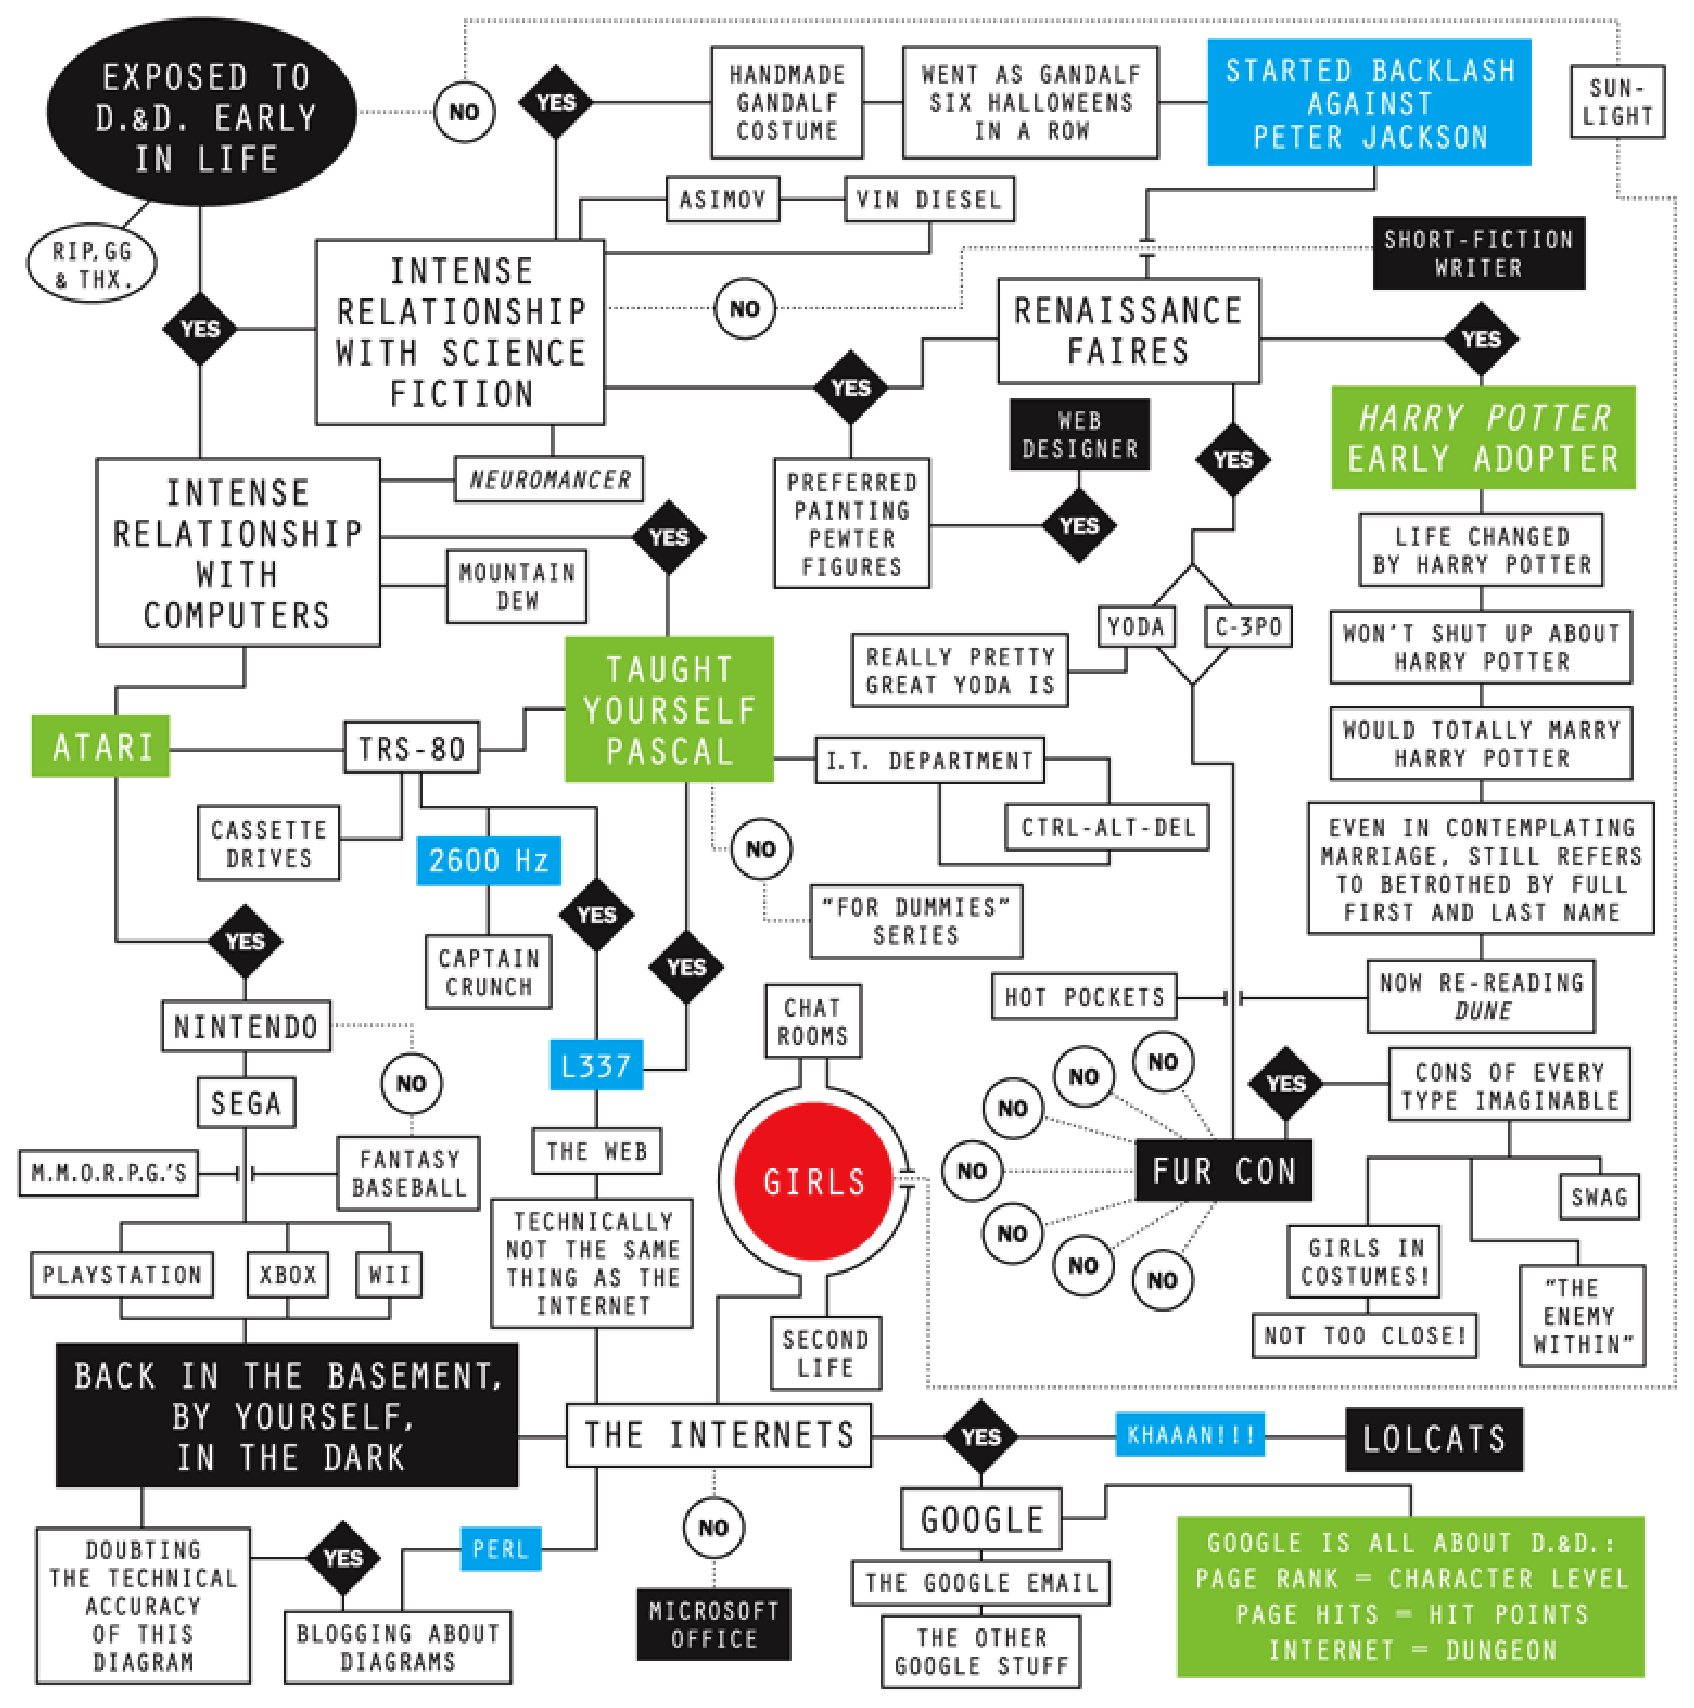
\includegraphics[width=0.7\textwidth]{\dir/figs/geek_flow_chart_nyt.eps}
  \caption{an example figure...}
  \label{fig.example}
\end{figure}

\renewcommand{\dir}{../chapter2/chapter/}
\chapter{Adaptive transition kernels for Bayesian phylogenetics}
\epigraph{ 
Monte Carlo is an extremely bad method; it should be used only when all alternative methods are worse.
}{Alan Sokal (1955-) in \textit{Monte Carlo Methods in Statistical Mechanics: Foundations and New Algorithms} (1996).}


\section{Introduction}	
\label{sec:intro_ch2}

In Bayesian phylogenetics one is usually interested in computing the posterior distribution
\begin{equation}
\label{eq:posterior}
 p(t, \boldsymbol b, \boldsymbol \theta | D) = \frac{f(D | t, \boldsymbol b, \boldsymbol \theta ) \pi(t, \boldsymbol b, \boldsymbol \theta )}{\sum_{t_i \in \mathbb{F}} \int_{\boldsymbol B}\int_{\boldsymbol \Theta} f(D | t_i, \boldsymbol b_i, \boldsymbol \theta ) \pi(t_i, \boldsymbol b_i, \boldsymbol \theta ) d\boldsymbol\theta d\boldsymbol b_i}\:,
\end{equation}
where $D$ is observed data and $t \in \mathbb{F}$ is a fully-ranked tree topology associated set of branch lengths $\boldsymbol b$. %TODO: maybe $\boldsymbol b(t)$?
Finally $\boldsymbol \theta$ is a set of parameters such as substitution model parameters, migration rates, heritability coefficients, etc.
In many applications, the aim is to construct time-calibrated phylogenies, i.e. phylogenetic trees whose branch lengths are measured in units of calendar time.
In particular, one might have sequences sampled through time (heterochronous/serially-sampled) which enable direct estimation of the rate of evolution and reconstruction of past population dynamics~\citep{Drummond2002, Drummond2005}.
These types of data sets pose additional challenges to inference because they impose constraints\footnote{More specifically temporal precedence constraints.} on the space of valid trees~\citep{Stadler2013}.

\subsection{MCMC in phylogenetic space}
\label{sec:tree_mcmc}

One of the main features of the Bayesian  approach is to allow parameter inference and hypothesis testing whilst accommodating phylogenetic uncertainty~\citep{Suchard2001, Huelsenbeck2002, Lemey2014, Cybis2015, Baele2015, Baele2017}.
This treatment of uncertainty is achieved by integrating (marginalising) over the space of phylogenies, a task which depends crucially on efficiently traversing tree space.
Even for the simplest models, the distribution in~(\ref{eq:posterior}) cannot be computed analytically requiring numerical approximation, usually accomplished through Markov chain Monte Carlo (MCMC).
The use of MCMC for Bayesian methods in phylogenetics has grown steadily since its introduction in the late 1990s and early 2000s~\citep{Kuhner1995,Sinsheimer1996, Rannala1996, Yang1997, Mau1999, Li2000, Suchard2001,Drummond2002}, with software packages such as Mr Bayes~\citep{Ronquist2012} and BEAST~\citep{Drummond2012,Suchard2018} becoming widely used by researchers in a broad range of disciplines~\citep{Murphy2001, Bouckaert2012, Lemey2014}.

The Metropolis-Hastings (MH) algorithm~\citep{Metropolis1953, Hastings1970} is a very popular MCMC technique due to its generality and ease of implementation.
% In MH, a Markov chain is constructed such that its limiting distribution is the desired posterior distribution. 
For ease of presentation, let $\tau = \{ t, \boldsymbol b\}$ be a phylogeny and $q_{\gamma}(\tau^\prime|\tau)$ be a conditional distribution indexed by a parameter $\gamma$ from which a new state $\tau^\prime$ can be proposed from a current state $\tau$.
We call $q_{\gamma}(\tau^\prime|\tau)$ a \textbf{candidate-generating distribution}.
It can be shown that accepting/rejecting a new state $\tau^\prime$ based on the ratio\footnote{I will drop the dependence of the posterior on $\boldsymbol\theta$ for convenience of notation. One should however keep in mind some parameters may be strongly correlated with the phylogeny $\tau$.} $A_{\gamma}(\tau | \tau^\prime) = min\left(1, \frac{p(\tau^\prime | D)q_{\gamma}(\tau|\tau^\prime)}{p(\tau | D)q_{\gamma}(\tau^\prime|\tau)}\right)$ leads to the desired distribution for a suitably constructed proposal mechanism.

There are no ``default'' choices for the candidate-generating distribution $q_{\gamma}(\cdot|\cdot)$; it must be chosen with the target distribution (in this case the Bayesian posterior) in mind.
Moreover, the efficiency of MCMC algorithms in approximating the target distribution depends crucially on the choice of transition kernel~\citep{Brooks2003,AlAwadhi2004,Yang2013,Thawornwattana2017}.
As argued by~\cite{Hoehna2012}, tree transition kernels are usually built in a relatively simplistic fashion, which in turn leads to inefficient exploration of tree space.
Moreover, most transition kernels proposed to date are not adaptive, i.e., the parameter(s) $\gamma$ cannot be adjusted during the Markov chain to achieve a desired acceptance probability~\citep{Haario2001}.
Given the clear advantage of adaptive MCMC over non-adaptive implementations for high-dimensional target distributions~\citep{Roberts2009, Baele2017}, the development of adaptive tree transition kernels could lead to substantial gains in performance.

\cite{Hoehna2008} developed new ``clock-constrained'' transition kernels to improve efficiency when dealing with time-calibrated trees. 
The authors point out that clock-constrained trees impose additional restrictions on the state space of the MCMC algorithm and hence that performance could be increased by developing transition kernels that took the extra information provided by tip dates.
They develop two such kernels: Fixed node-height Prune-and-Regraft (FNPR) and Intermediate Exchange (IE).
FNPR finds a ``target'' node (excluding the root and its two children) at random, prunes it and regrafts the resulting subtree at a ``destination'' node in the tree at the same height at random.
Intermediate Exchange is similar in spirit, but the regraft node  is not chosen uniformly. 
Instead, IE is constructed to prefer local rearrangements, by picking closer nodes with a higher probability (see below and section II in~\cite{Hoehna2008} for details).
A limitation of FNPR nor IE is that they are not adaptive.

\cite{Hoehna2012} explored more sophisticated ``guided'' tree transition kernels, inspired by Gibbs sampling~\citep{Geman1984}.
The idea behind their ``Metropolised'' Gibbs samplers is to maximise transition probability, i.e., the probability that the chain moves to a new state.
This is accomplished by prohibiting the current state as a proposed state, leading to a transition probability of one.
The kernels developed in~\cite{Hoehna2012} use a weighting scheme based on conditional clade probabilities (CCP) to guide transitions between trees.
A move to a tree with a lower CCP score is thus less likely, whilst a move that increases the score has a higher probability of being accepted.
A limitation of these Metropolised transition kernels is that CCP scores require normalisation over all trees~\citep{Larget2013} and hence can be cumbersome to calculate.

More recently,~\cite{Dinh2016} and~\cite{Fourment2017} develop ``guided'' candidate-generating mechanisms for on-line Bayesian phylogenetics via sequential Monte Carlo, which makes use of a surrogate function to make computations feasible.
While that is an active field of research, it relies on machinery not yet extended to the time-calibrated case.
Hence in this thesis and chapter I will focus on extending existing MH algorithms, which I will argue strikes a balance between computational efficiency and tractability.

To achieve maximum efficiency, a tree transition kernel needs to have the following characteristics: (i) be computationally cheap; (ii) be adaptive; (iii) traverse phylogenetic space quickly, i.e., have a high \textit{mixing rate}.
In this chapter I develop and study two simple, adaptive time-tree transition kernels, which we implement in the open source software package BEAST (\url{https://github.com/beast-dev/beast-mcmc/}).
I analyse performance in real as well as simulated data sets, focusing on the inference of time-calibrated phylogenies.
Technical details necessary to make some of the claims in this chapter precise are given in Section~\ref{sec:stx_properties}. %TODO: check if necessary

% \section{Technical details}
% \label{sec:tech}

\section{New time-tree transition kernels}
\label{sec:newKernels}

In this section I introduce two new candidate-generating densities that attain the properties discussed above while being specially designed for time-calibrated phylogenies.

\subsection{Preliminaries}
\label{sec:prelim}

I briefly lay out some notation and background that will be necessary for the presentation, with further details and more rigorous definitions already given in Chapter 1 (Section~\ref{sec:tree_space}).
Throughout this  chapter I will use $\boldsymbol\Psi$ to denote the parameter space encompassing topologies and branch lengths, henceforth called ``phylogenetic space'', and $\tau \in \boldsymbol\Psi$ to denote a bifurcating, rooted tree with branch lengths on $n$ taxa\footnote{What~\cite{Drummond2015} call a ``fully ranked'' tree.}.
Let $\mathbf{B}(\tau) =\{b_1, b_2, \ldots, b_{2n-2}\}$ be the set of branch lengths of $\tau$.
It is possible to compute the height of each node using a mapping $h(\cdot)$ such that $\mathbf{H}(\tau) = \{h_1, h_2, \ldots, h_{2n-1}\}$ is the set of node heights for all nodes (internal and external) in $\tau$.
Here we will define $h(i) = l_{max} - l_i$ and $l_i = \sum_{k \in \mathbf{W_i}} b_k$, where $\mathbf{W_i}$ is the minimal path between node $i$ and the root $\rho$ and $l_{max}$ is the maximum of these shortest paths.
It is also convenient to define $P_i$, $G_i$ and $S_i$ as the parent, grandparent and sibling of node $i$, respectively.
With this notation in mind, call $p_i = h(P_i)-h(i)$, $g_i = h(G_i)-h(P_i)$ and $q_i = h(P_i)-h(S_i)$ the corresponding branch lengths.
The most recent common ancestor of nodes $i$ and $j$, $\text{mrca}_{ij}$ is the first node in which the paths $\mathbf{W_i}$ and $\mathbf{W_j}$ intersect.
Finally, let $\Delta_{ij} = 2h(\text{mrca}_{ij}) - [ h(i)  + h(j) ]$ be the patristic (path) distance between nodes $i$ and $j$ on the phylogeny.

\subsubsection*{SubTreeJump} 

The first transition kernel I propose, \textit{SubTreeJump} (STJ)\footnote{An alternative name for STJ is generalised fixed node height prune and regraft, gFNPR.}, is similar in spirit to both Intermediate Exchange and FNPR.
STJ extends IE by introducing a tuning parameter $\alpha$ that controls how local rearrangements are.
The idea is to make the probability of moving node $i$ to $j$ proportional to $\Delta_{ij}^\alpha$ instead of $\Delta_{ij}$ as in Intermediate Exchange.
The necessary steps to perform a SubTreeJump operation on $\tau$ in order to propose a phylogeny $\tau^\prime$ are described in detail in Box~\ref{alg:stj} and an illustration is provided in Figure~\ref{fig:stj}.
This allows one to favour bold moves away from $i$ ($\alpha > 0$) or more conservative moves closer to $i$ ($\alpha < 0$).
Notice that SubTreeJump is equivalent to FNPR for $\alpha = 0$.
One can then define the SubTreeJump candidate-generating density as $q_{\alpha}(\tau^\prime | \tau) = Pr(i\to j)$.

\begin{algorithm}[!ht]

\setcounter{AlgoLine}{-1}

 Excluding the root and its children, pick a node $i$ in  $\tau$ uniformly at random, i.e., with probability $1/(2n-4)$;
 
 Determine $P_i$ and compute $h(P_i)$;
 
 Construct the set of destination nodes $\mathbf{D_i} = \{ d : h(d) \leq h(P_i) < h(P_d) \}$;
 
 For all $k \in \mathbf{D_i}$, compute $l_{ik}$;
 
 For some fixed $\alpha \in \mathbb{R}$, pick a node $j$ with probability $Pr(i\to j) = \frac{\Delta_{ij}^{\alpha}}{\sum_{d \in \mathbf{D_i}}\Delta_{id}^{\alpha}}$;
 
 Prune the phylogeny at $P_i$ and regraft the resulting subtree at $P_j$, creating a new phylogeny $\tau^\prime$. 
 
 \caption{SubTreeJump transition kernel.}
 \label{alg:stj}
\end{algorithm}

Note that while for $\alpha = 0$ the move is symmetric~\citep{Hoehna2008}, for $\alpha \neq 0$ the density $q_{\alpha}(\cdot|\cdot)$ is not, since for two arbitrary nodes $i$ and $j$  whilst the sets $\mathbf{D_i}$ and $\mathbf{D_j}$ coincide ($|\mathbf{D_i}| = |\mathbf{D_j}|$), the distances between nodes usually do not.
Hence one needs to compute the \textit{Hastings ratio} $q_{\alpha}(\tau|\tau^\prime)/q_{\alpha}(\tau^\prime|\tau)$.
To get a reverse move from $\tau^\prime$ back to $\tau$, one needs to pick the original target node $i$  -- which is guaranteed to exist in $\mathbf{D_j}$ -- as a destination. 
The Hastings ratio is then\footnote{Note that I omit the node-picking probability $1/(2n-4)$ because it is the same for both moves. If one were to devise a kernel with non-uniform node-picking probabilities, these would have to be included in the Hastings ratio.}
\begin{align}
 \frac{q_{\alpha}(\tau| \tau^\prime)}{q_{\alpha}(\tau^\prime| \tau) }  &= \frac{\Delta_{ij}^{\alpha}}{\sum_{d^\prime \in \mathbf{D_j}}\Delta_{id^\prime}^{\alpha}} /\frac{\Delta_{ij}^{\alpha}}{\sum_{d \in \mathbf{D_i}}\Delta_{id}^{\alpha}}, \nonumber \\
 &  = \frac{\sum_{d \in \mathbf{D_i}}\Delta_{id}^{\alpha}}{\sum_{d^\prime \in \mathbf{D_j}}\Delta_{jd^\prime}^{\alpha}}.
\end{align}

I note two limitations of this transition kernel.
First, because $\mathbf{H}(\tau)$ is ultimately discrete for any given $\tau$, not any acceptance probability is attainable.
This ``granularity'' of the kernel density causes problems for most adaptation schemes because the dependence of the acceptance probability on the indexing parameter is implicitly assumed to be smooth (see Section~\ref{sec:STJadap}).
% becomes irrelevant for large trees, but remains an issue for very small trees ($<10$ taxa).
Secondly, SubTreeJump on its own does not necessarily induce an irreducible Markov chain on the space of rooted topologies  -- see Section~\ref{sec:stx_properties} for a counterexample/proof.
This can be easily remedied by combining STJ with branch length candidate-generating mechanisms.
Since STJ  (and FNPR) does not change node heights or numbers of lineages, it does not change the density under the coalescent prior,~\textit{i.e.} $\pi(\tau) = \pi(\tau^\prime)$.
Whether this is a desirable property is an open question.
The disconnect between proposals in topological space and branch length space could be undesirable due to it failing to account for the dependence between topology and branch lengths.

\begin{figure}[!ht]
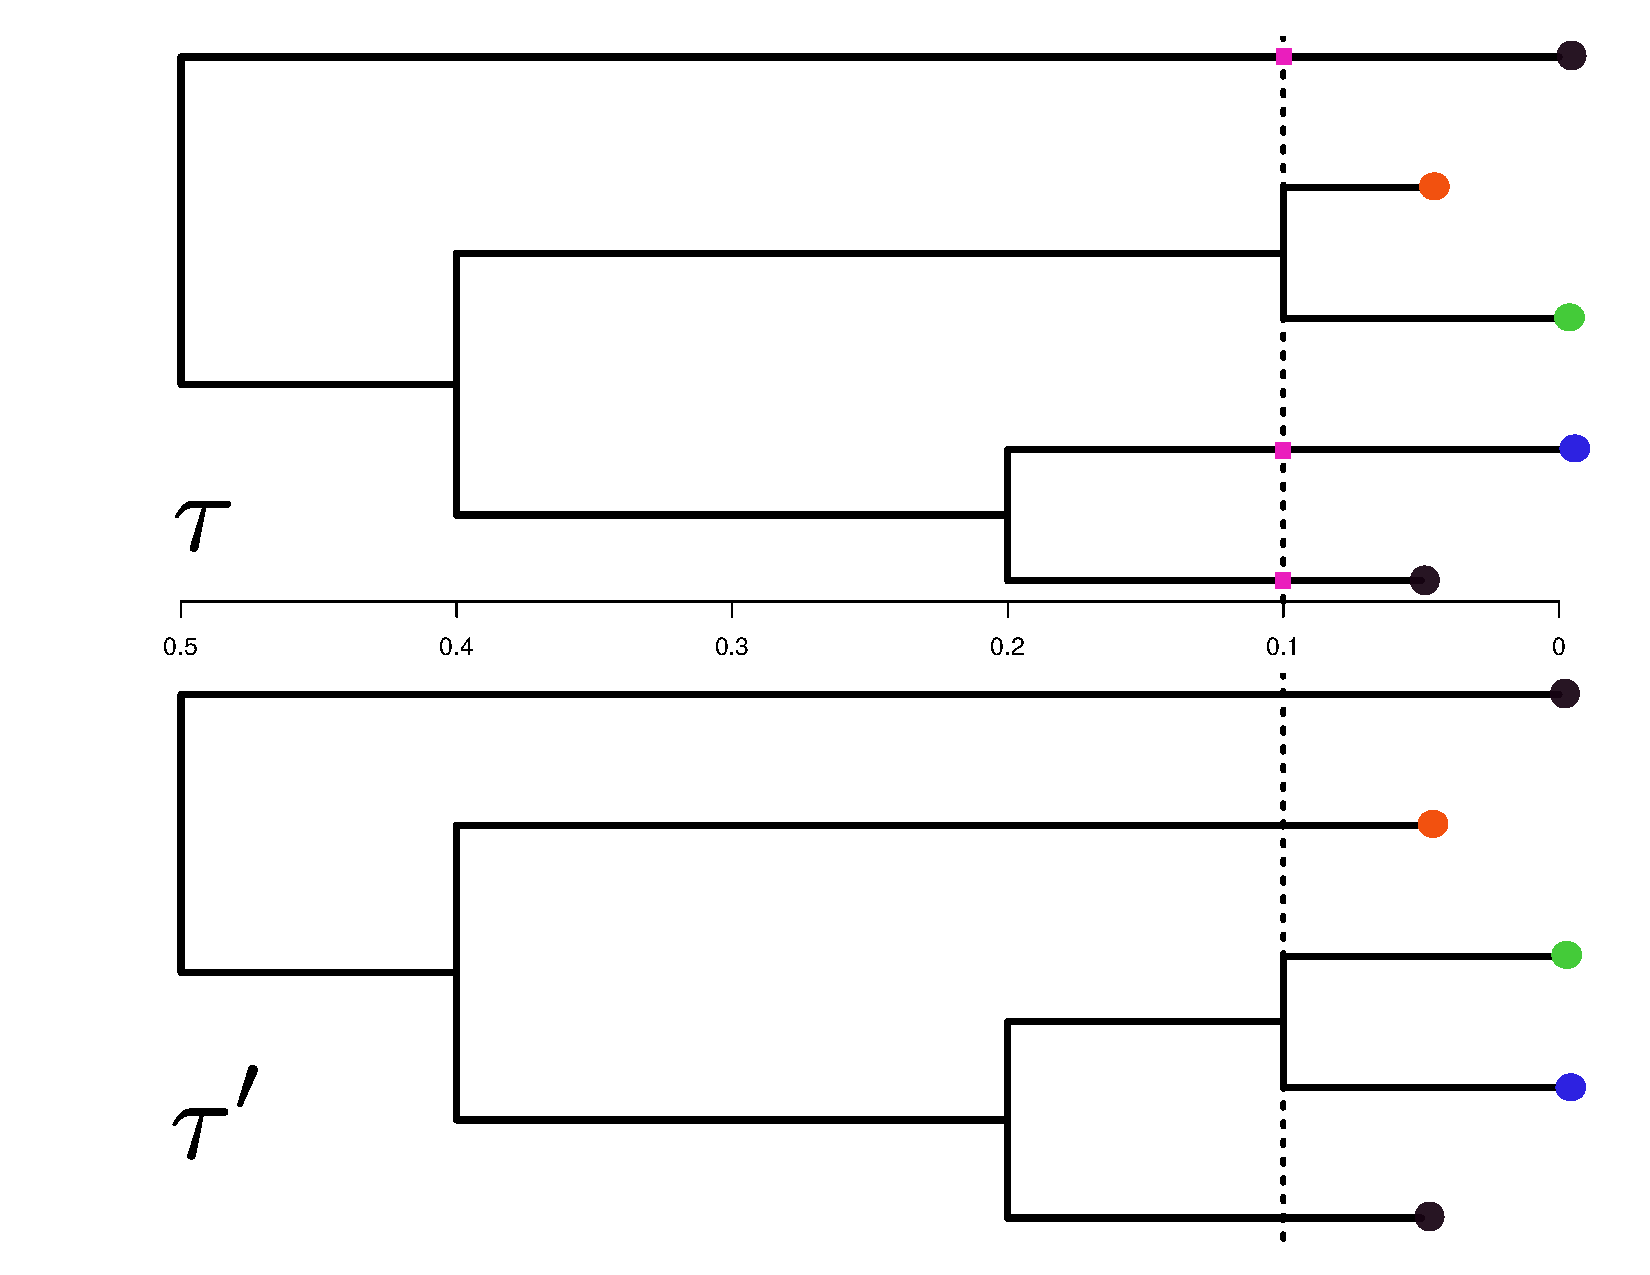
\includegraphics[scale=0.5]{\dir/figs/STJ.pdf}
 \caption[Schematic representation of a SubTreeJump proposal]{\textbf{Schematic representation of a SubTreeJump proposal}. The target node (green) is picked, we find all the nodes (or positions along branches) that intersect at the height of its parent (pink squares) and then a destination is picked with probability as described in the text.
 Other nodes are coloured so the reader can easily identify the changes.}
 \label{fig:stj}
\end{figure}


\subsubsection*{SubTreeLeap} 

Ideally, we would like to have a single adaptive transition kernel to update topology and branch lengths simultaneously.
To this end I propose~\textit{SubTreeLeap} (\verb|STL|), a transition kernel based on patristic distances.
The central idea behind \verb|STL| is to move a node $i$ to new location in the tree that is at most at (patristic) distance $\delta$ from $i$.
To this end, one first draws the distance $\delta$ from a distribution $\kappa(\delta | \sigma)$ indexed by a parameter $\sigma$, henceforth called the \textit{distance kernel}.
One then finds the set $\mathbf{D_i(\delta)}$ of all the destination nodes that are at distance $\delta$ from $i$, and picks the destination $j$ uniformly at random from these.
The regraft height of $j$ -- at $P_j$ -- will be $h^\prime = 2 h(\text{mrca}_{ij}) - h(P_i) -\delta$.
See Box~\ref{alg:stl} for details.

\begin{algorithm}[!ht]
\setcounter{AlgoLine}{-1}
\SetKwProg{Fn}{Function}{}{}
\SetKwInOut{In}{Input}
\SetKwInOut{Out}{Output}

     Excluding the root, pick a node $i$ in  $\tau$ uniformly at random, i.e., with probability $1/(2n-2)$;
     
     Draw a patristic distance $\delta$ from the distance kernel $\kappa(\delta | \sigma)$;
     
     Find the set of destination nodes $\mathbf{D_i}(\delta) \leftarrow getDestinations(\tau, i, \delta)$;
     
%      \eIf{$\mathbf{D_i}(\delta) = \O$}{
%      Prune $p_i$ and regraft it at height $h_{b} =  h(p_i) - \delta$, creating a new tree $\tau^\prime$.
%      }{
     Pick a node $j \in \mathbf{D_i}(\delta)$ with probability $Pr(i\to j) = 1/|\mathbf{D_i}(\delta)|$;
     
     Prune the tree at $P_i$ and regraft it at $P_j$, creating a new tree $\tau^\prime$. %% TODO: should it be "prune the tree at $i$" ??
%      }
     
     \Fn{getDestinations}{
     \In{ A tree $\tau$, a node $i$ and a scalar $\delta$.}
     \Out{A set $\mathbf{D_i}(\delta) = \{c  : d(c, i) \leq \delta \}$.}
     \setcounter{AlgoLine}{-1}
     
      Determine $P_i$, $S_i$ and $G_i$;
      
      Compute $p_i = h(P_i)$;
      
      Compute $h_{b} =  p_i - \delta$; 
     
      \If{$h_b > h(i)$}{
         Go down the subtree subtended by $s_i$ and find all nodes that intersect at height $h_b$ constructing the set $\mathbf{D^{(b)}_i} = \{ d : h(d) \leq h_b < h(P_d) \}$\;
    }
      Compute $h_{a} =  h(P_i) + \delta$;
      
      Walk up to the root and find all nodes that intersect at height $h_a$ constructing the set $\mathbf{D^{(a)}_i} = \{ d : h(d) \leq h_b < h(P_d) \}$\;
      
    \Return $\mathbf{D_i}(\delta) = \mathbf{D^{(b)}_i}(\delta) \cup \mathbf{D^{(a)}_i(\delta)} $
     }
     
 \caption{SubTreeLeap transition kernel.}
 \label{alg:stl}
\end{algorithm}

\begin{figure}[!ht]
\begin{center}
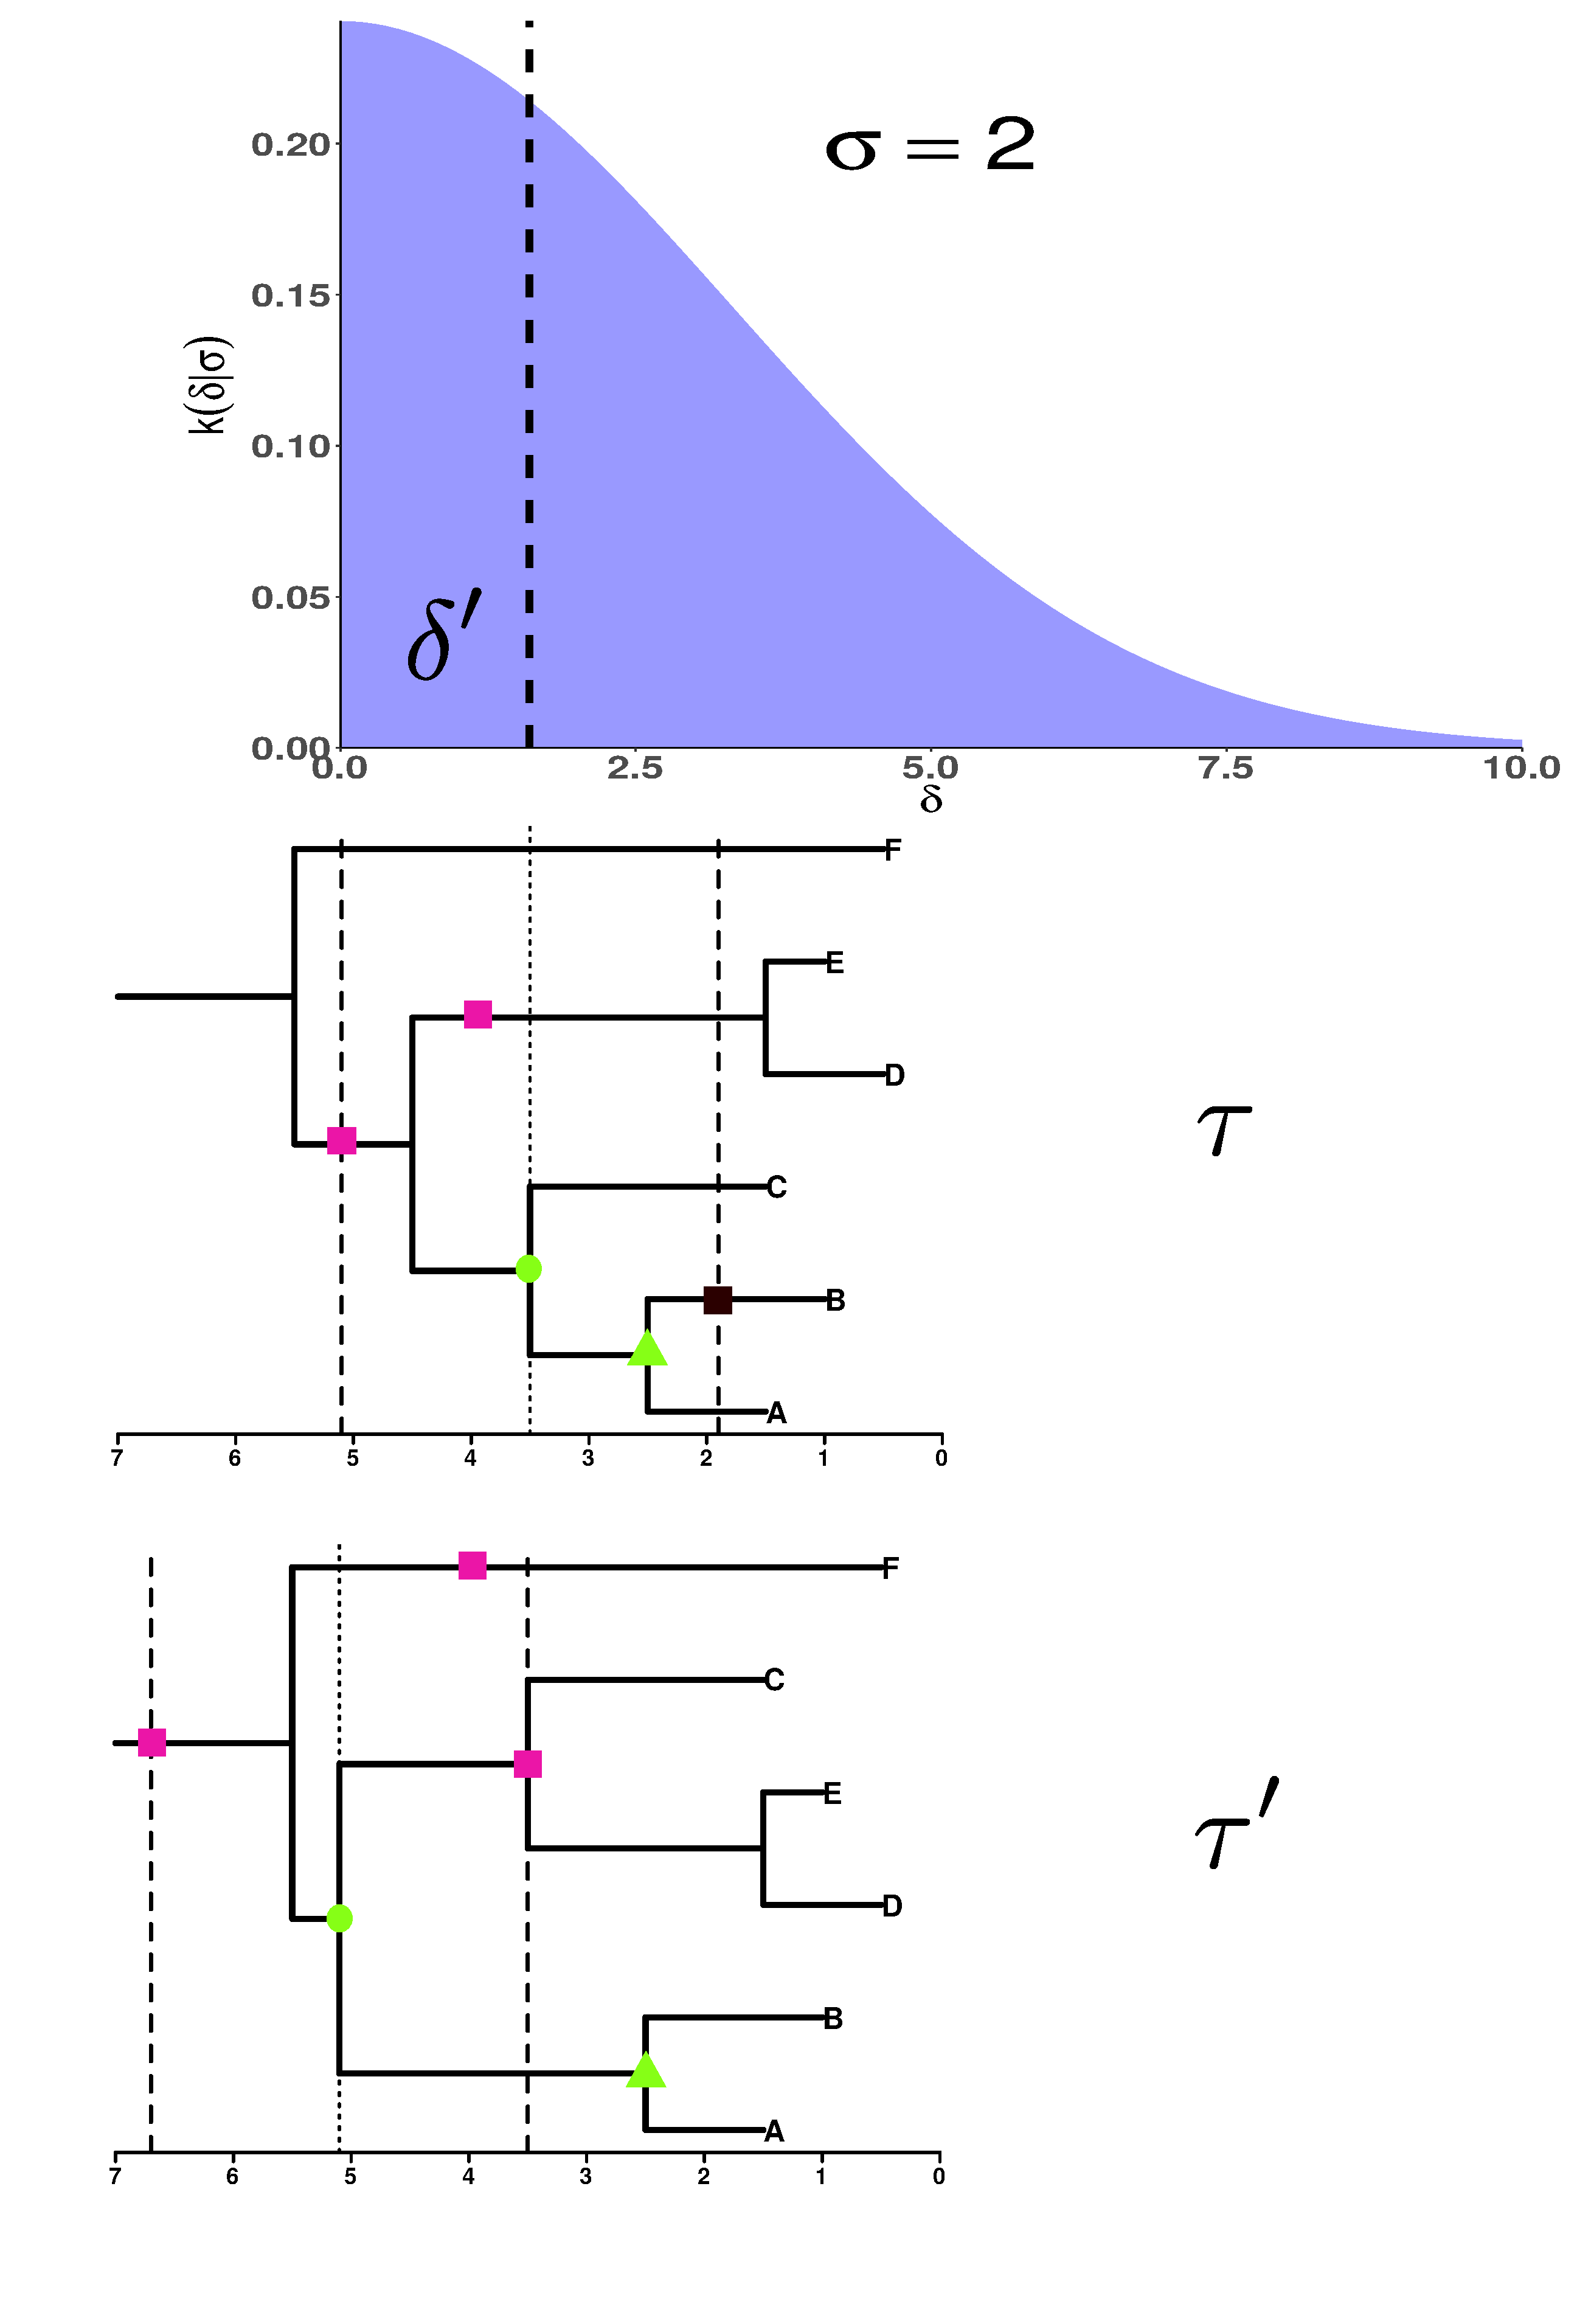
\includegraphics[scale=0.20]{\dir/figs/STL_new.pdf} 
\end{center}
% \begin{center}
% \subfigure[\textbf{Symmetric example}]{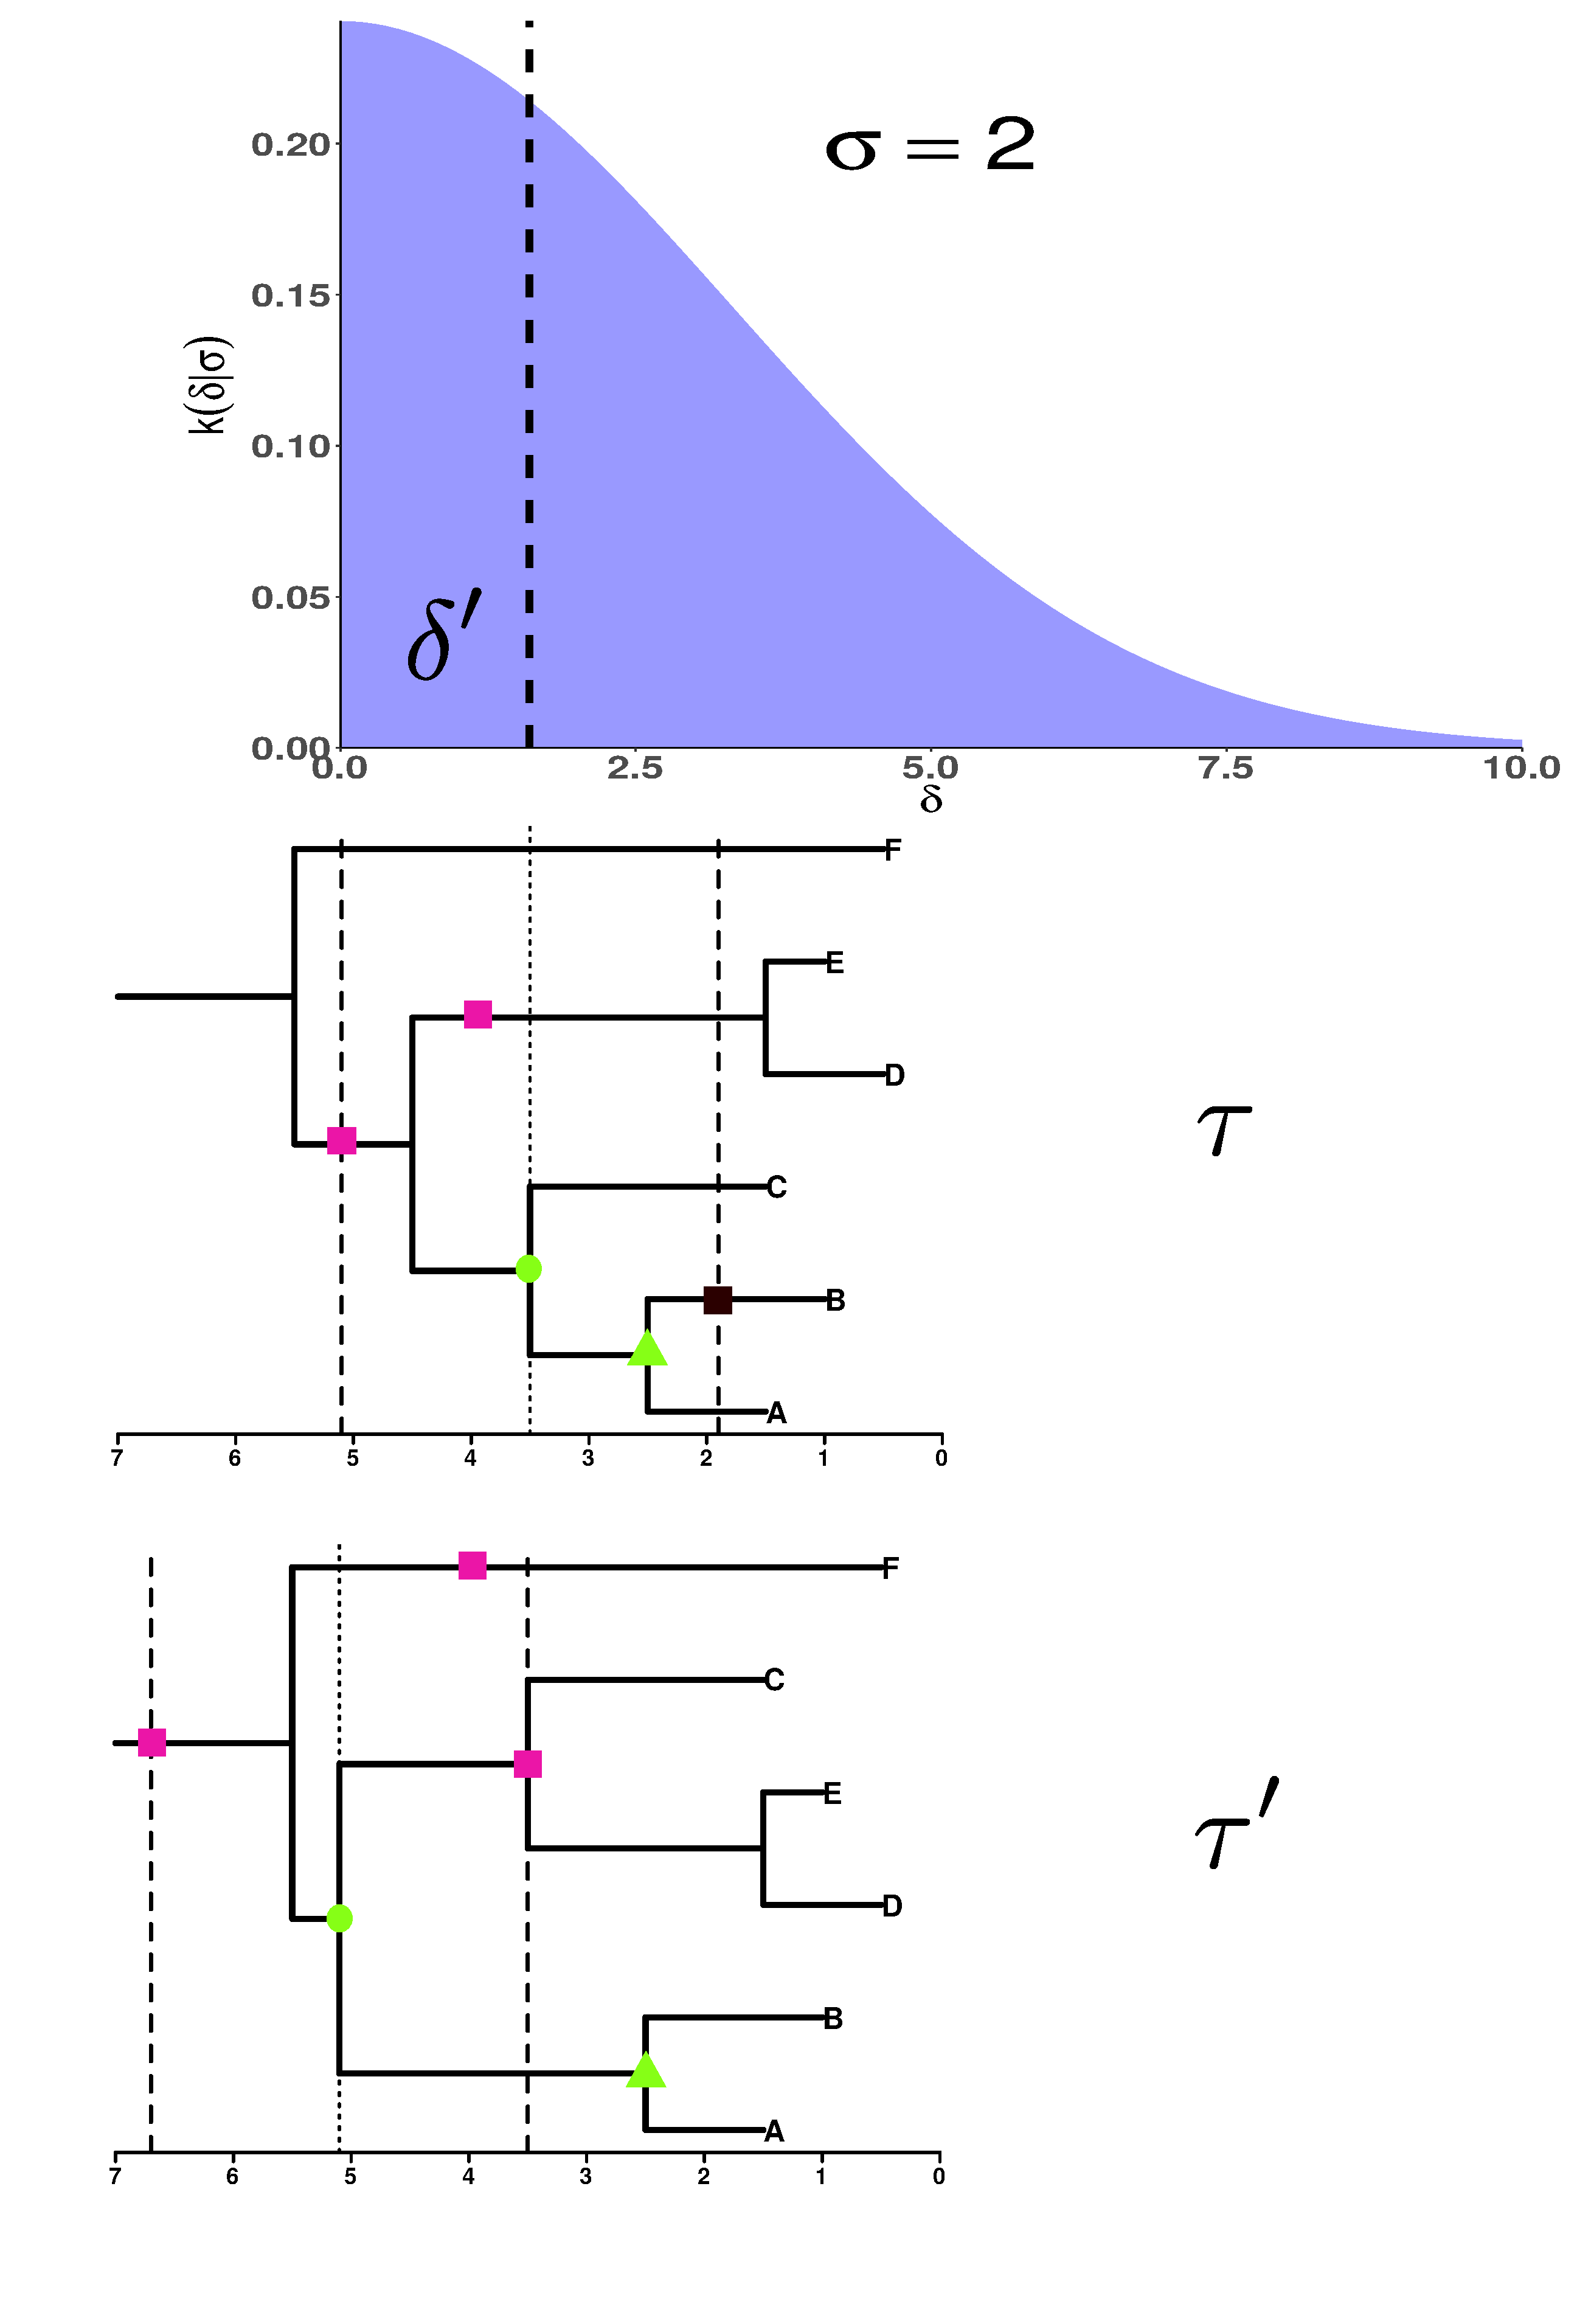
\includegraphics[scale=0.4]{\dir/figs/STL_new.pdf} }%
% \subfigure[\textbf{Asymmetric example}]{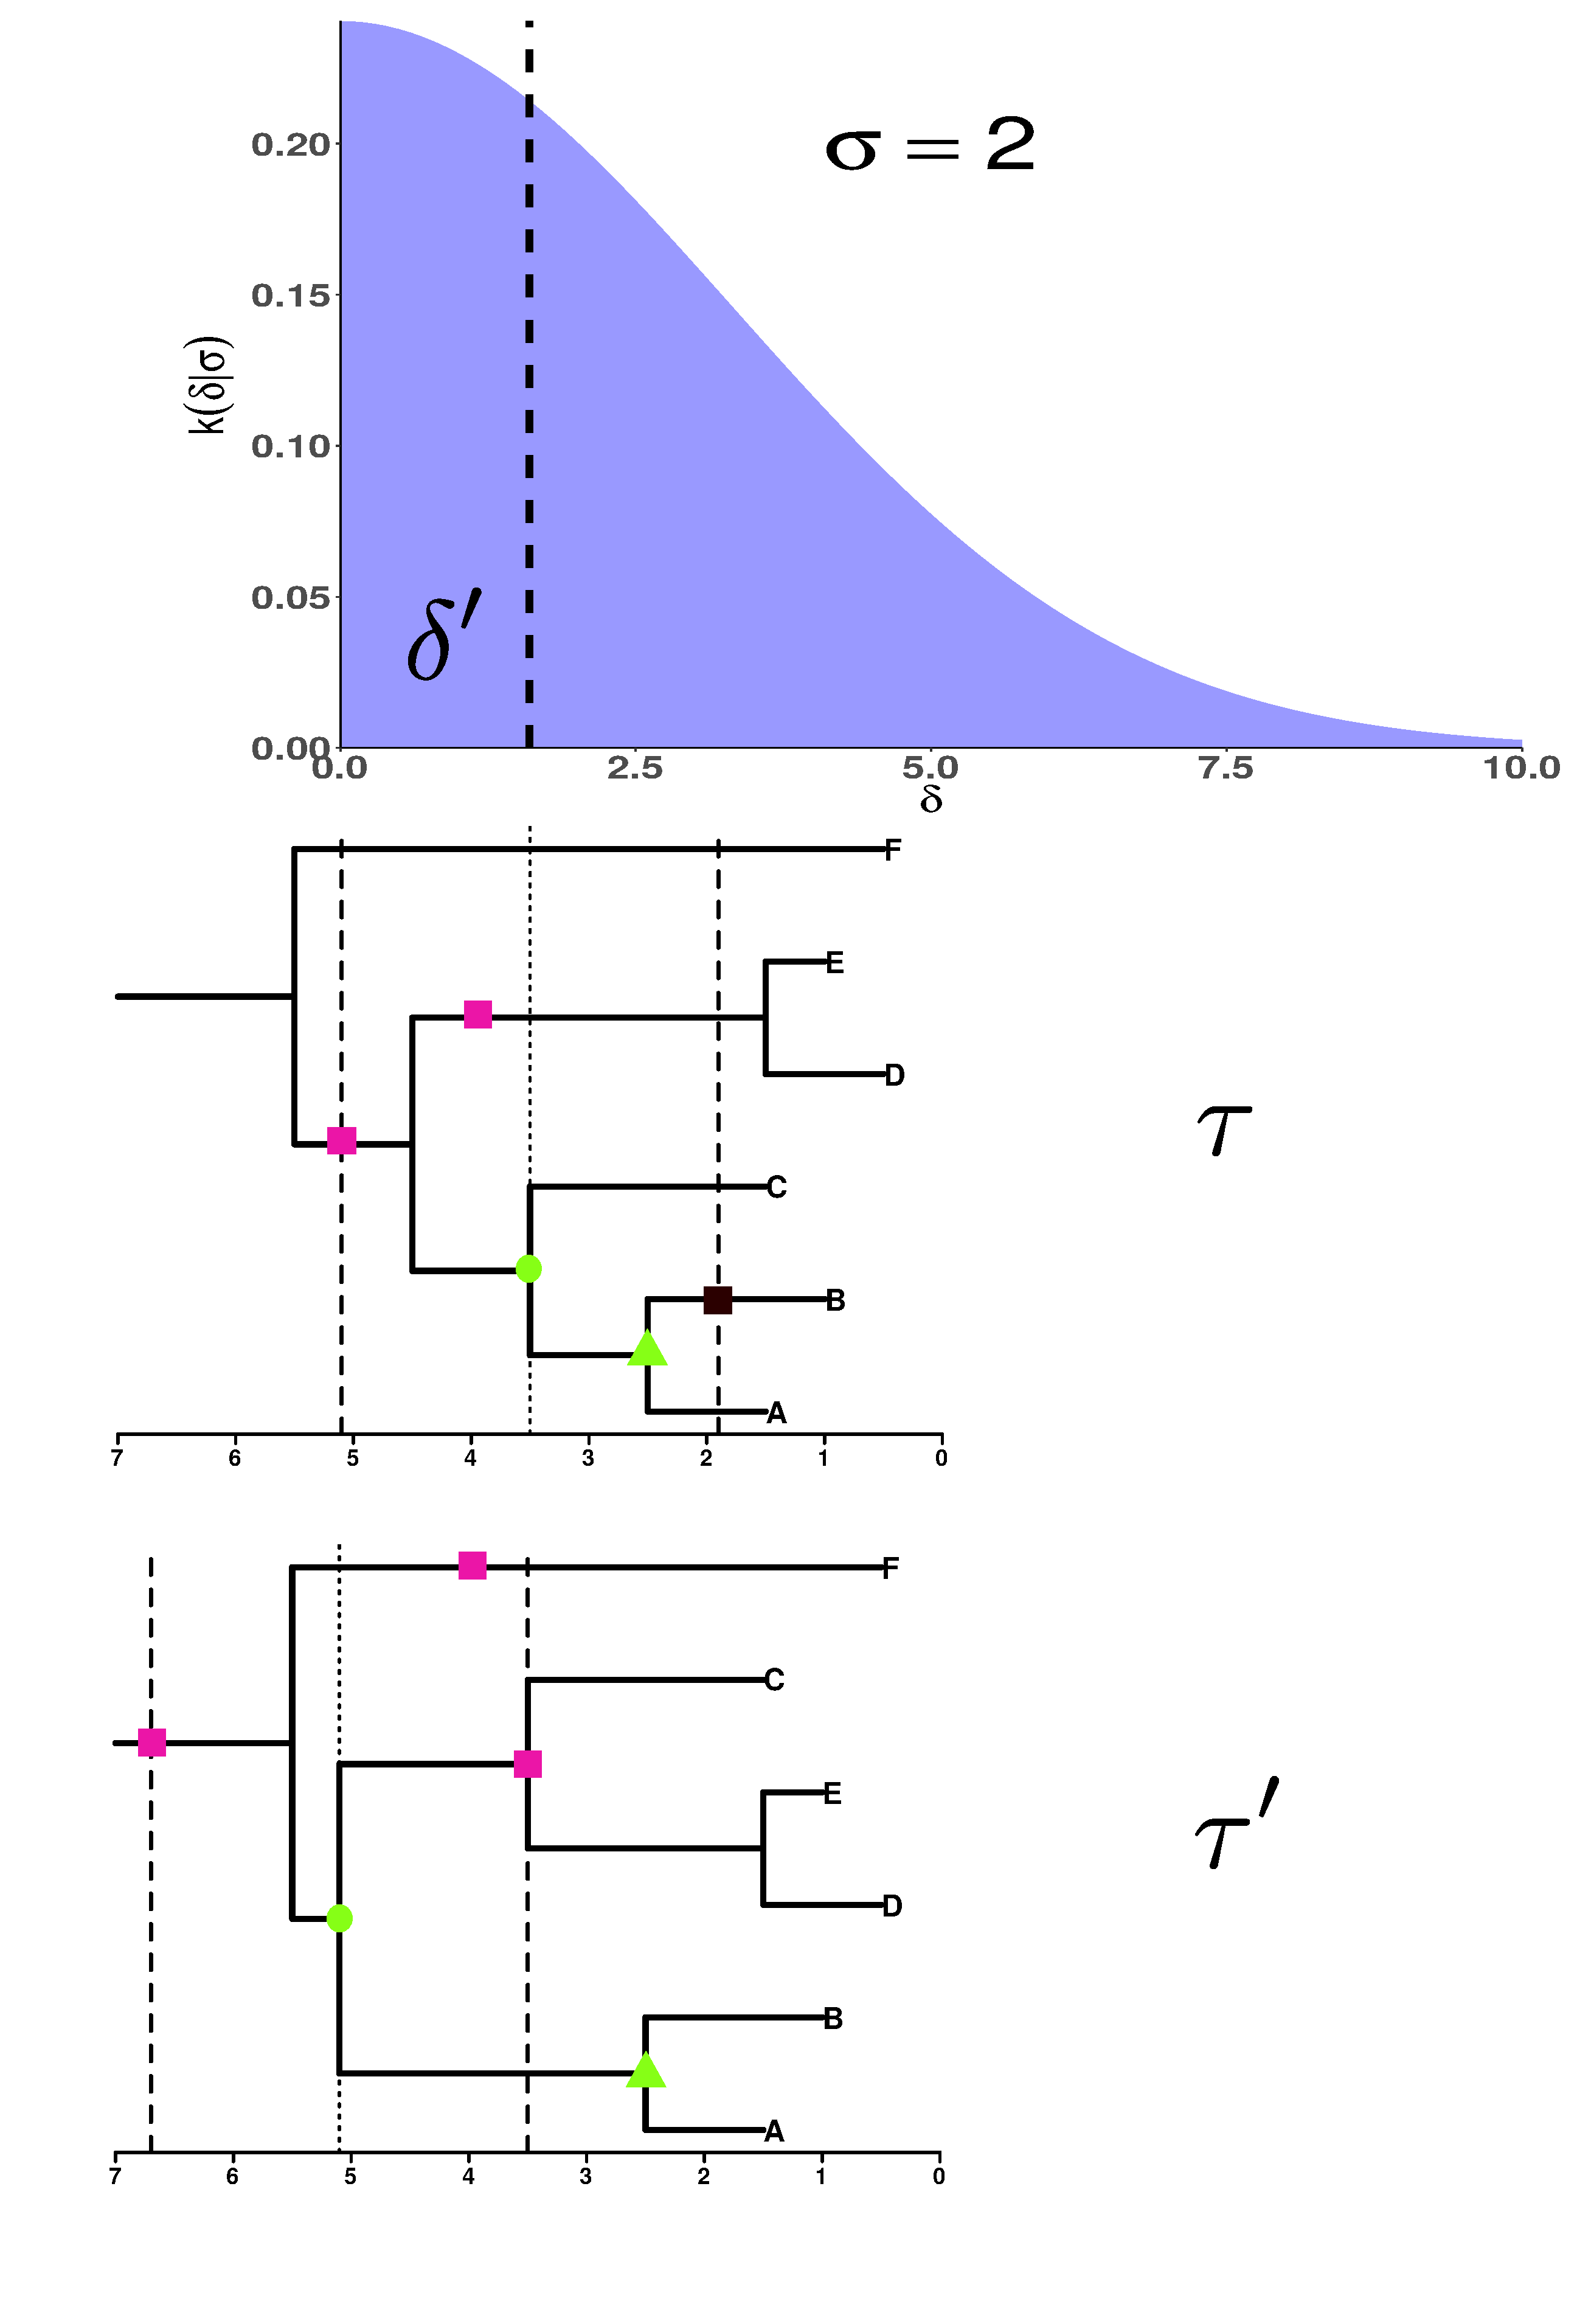
\includegraphics[scale=0.4]{\dir/figs/STL_new.pdf} }  
% \end{center}
 \caption[Schematic representation of a SubTreeLeap proposal]{\textbf{Schematic representation of a SubTreeLeap proposal}.
 SubtreeLeap operation with size  $\delta^\prime = 1.6$ on $\tau$ to obtain the proposal phylogeny $\tau^\prime$.
 Target node represented by the green triangle and the height of its parent (green circle) marked by a dotted line; valid destination nodes marked with pink squares, invalid (prohibited) destinations are marked with black squares.
%  Starting from a phylogeny $\tau$, excluding the root pick a node $i$ uniformly at random (red triangle) and distance $\delta^\prime = 1.6$ from the kernel $\kappa(\delta | \sigma)$ (blue distribution).
%  Find the possible destination(s) that are distance $\delta^\prime$ from $P_i$, whose height is marked with a dotted line.
%  The destination nodes are represented by  pink squares, their heights marked by dashed lines.
%  Prune $P_i$ and regraft it at the parent of the chosen destination, making the new phylogeny $\tau^\prime$.
%  To get back from $\tau^\prime$ to $\tau$ one needs to pick the appropriate node (with the same probability as before) and then compute the destination set following the same procedure.
 Notice that (a) there is always a destination node above the root and (b) the Hastings ratio would be $ \frac{|\mathbf{D_i}(\delta)|}{|\mathbf{D_j}(\delta^\prime)|} = 2/3$.
 See text for details.
}
 \label{fig:stl}
\end{figure}

Like SubTreeJump, SubTreeLeap is also not symmetric, hence we need to compute the Hastings ratio $q_{\sigma}(\tau|\tau^\prime)/q_{\sigma}(\tau^\prime|\tau)$.
In order to get back to $\tau$ from $\tau^\prime$ one would first need to draw the same distance $\delta^\prime = \delta$ from $\kappa(\cdot)$. 
Then one needs to realise that the original node $i$ is guaranteed to exist in the set of destinations $\mathbf{D_j}$ -- but $\mathbf{D_j} \neq \mathbf{D_i}$.
Hastings ratio is then 
\begin{align}
 \frac{q_{\sigma}(\tau|\tau^\prime)}{q_{\sigma}(\tau^\prime|\tau)} & = \frac{1}{|\mathbf{D_j}(\delta^\prime)|}/\frac{1}{|\mathbf{D_i}(\delta)|},  \\ \nonumber
 & = \frac{|\mathbf{D_i}(\delta)|}{|\mathbf{D_j}(\delta^\prime)|}
\end{align}
One needs to draw the exact same distance $\delta^\prime = \delta$ to be able to get the original node in the destination set and hence produce $\tau$ from $\tau^\prime$.
This means the densities $\kappa(\delta^\prime | \sigma)$ and $\kappa(\delta| \sigma)$ -- independently of the choice of distance kernel\footnote{As long as $\kappa(\cdot)$ is strictly positive and unbounded (see Remark~\ref{rmk:stl_irreducible_F}).} --  cancel out in the Hastings ratio leaving only the discrete component to be computed.

This construction is complicated and deserves a bit more consideration.
Let $m_i = \min(g_i, q_i)$ and consider $j$ as a virtual destination node.
Depending on the magnitude of the distance $\delta$, a range of rearrangements is possible:

\begin{enumerate}[label=\Alph*)]
 \item Complete slide move (CSM): if $\delta < p_i$ and $\delta < m_i$, the regraft point will lie either on the branch subtending $P_i$ or the one subtended by $P_i$;
 \item Partial slide move (PSM): if $\delta < p_i$ but $\delta > m_i$, there is only one destination -- above $P_i$ -- because moves that extend $p_i$ below are forbidden due to the restrictions imposed by fixed sampling times.
 \item Same subtree topological move (SSTM): if $\delta > p_i$ and/or $\delta > m_i$ but $\delta < h(\rho)-h(P_i)$ a topological rearrangement will occur, but will change only the subtree\footnote{The root $\rho$ has two children, $L$ and $R$, and if $P_i \neq \rho$ it is either one of $L$ and $R$ or the child of exactly one of $R$ or $L$.} that contains $P_i$.
 Similar to the above, a STM can be either ``complete'' or ``partial'', depending on the constraints imposed by $m_i$;
 \item Cross tree (topological) move (CTM): on the other hand if $\delta > h(\rho)-h(P_i)$ the destination set $\boldsymbol D_i(\delta)$ will only include destinations on the subtree across $i$ from the root.
 \end{enumerate}

For a CSM $h^\prime$ is either $h(P_i) + \delta$ or $h(P_i) - \delta$  with probability $1/2$.
The rationale above is valid even when $P_i$ is the root node, meaning the tree can be indefinitely extended above --\textit{i.e.} backwards in time\footnote{This does however require a bit of an abuse of notation, since the root does not have a parent node, but we would have to have $P_\rho = \rho$.}.
If $\delta > \max_{j} d(P_i, j)$ the height $h^\prime$ is bigger than the height of the root (tree height) and there will be no destinations on the opposite subtree.
In this case, there is only one destination node, above the root, and the parent of $i$, $P_i$, becomes the root (see Figure~\ref{fig:stl}).
This is in stark contrast with the default set of operators available in BEAST, where one needs a specific move to change the height of the root.
As a trade-off however, \verb|STL| will only change the root height occasionally.

An interesting property of \verb|STL| is that the scaling parameter $\sigma$ can be set in time units, which makes it easier to tune the parameter to be commensurate with the expected age of the root, for instance.
This is particularly helpful when setting the initial value for $\sigma$ (before chain adaptation) if one has a rough guess of the evolutionary rate.
Updating the root height is important because in phylodynamics the height of the root carries information on the time of origin of the most recent common ancestor of the circulating lineages, and sometimes the epidemic (see e.g.~\cite{Gire2014}).

\subsection{The posterior distribution in Bayesian phylogenetics}
\label{sec:prior_maths}

Before analysing the properties of a~\verb|STL| (or \verb|STJ|) Markov chain in phylogenetic space, it would be convenient to study some properties of the target distribution $p(\cdot)$ in order to understand the challenges it poses to MCMC algorithms.

Recall that $\boldsymbol\Psi = \mathbb{F} \times \mathbf{S}$,~\textit{i.e.}, phylogenetic space, is an infinite space composed of a finite discrete component of (fully-ranked)~\textit{topologies} $\mathbb{F}$, and a continuous space of inter-coalescent intervals $\mathbf{S}$ (branch lengths can also be used).
Any analysis of Markov chains on this space needs to take into account the projection of the resulting measure on both spaces, as well as consider their interaction~\citep{Gavryushkin2016b}.
For instance, one can analyse the projection of a random walk on $\boldsymbol\Psi$ by looking at the induced (marginal) random walk on $\mathbb{F}$, represented by the SPR graph (see Chapter 1).
\cite{Gavryushkin2016} claim about the MCMC on space of phylogenies: ``mixing over these discrete structures is the primary obstruction to MCMC convergence'' (pg. 1102).
While I do agree with the authors, it is also important to point out that the~\textbf{interaction} between branch lengths and topology may also play a role.
This is because even if $t$ and $\boldsymbol b$ are assumed independent~\textit{a priori}\footnote{A dubious assumption, made for computational tractability.}, they tend to inextrincably correlated~\textit{a posteriori}\footnote{The existence of a particular configuration of branch lengths $\boldsymbol b$ is defined only conditional on an underlying topology $t$.}.
The main purpose of the candidate-generating mechanisms proposed here is to account for this interaction when proposing new states in the Markov chain.
In this section I shall present some observations about the target distribution and its support $\boldsymbol\Psi$ in the same spirit as section 6.1 in~\cite{Dinh2017}, but with the goal of analysing the theoretical properties of phylogenetic transition kernels with special focus on the ones presented here.

Under mild regularity conditions, the likelihood is continuous and smooth up to the boundary of the BHV space; see~\cite{Dinh2017} for proofs.
This  property holds if the phylogenetic prior itself attains the property that it is smooth and continuous up the boundary~\citep[Assumption 2.3]{Dinh2017},
which I show to be the case for parametric coalescent priors (see Equation~\ref{eq:coal_prior}).
In general, any function $\mu : \boldsymbol S \times \boldsymbol K \to [0, \infty]$ such that $\sum_i\int_{\mathbb{R}^{2n-1}} \mu (\boldsymbol s, \boldsymbol k_i) d\boldsymbol s < \infty$ with $\frac{\partial \mu}{\partial \boldsymbol s} \in \mathcal{C}^1$  will fulfill these conditions.   

Recall that the density under the parametric constant population coalescent is \cite[eq 5.1, pg. 81]{Drummond2002b}:
\begin{equation}
\label{eq:coal_prior_short} 
\pi_0(\tau| N_e) = \frac{1}{N_e^{n-1}}\exp\left(-\frac{1}{(2N_e)^{2n-2}}\sum_{j=2}^{2n-1} k_j(k_j -1)(s_j - s_{j-1}) \right).
\end{equation}

It is clear that $\pi_0(\tau| N_e)$ is differentiable with respect $\boldsymbol s$.
In addition, $\boldsymbol k$ does not change inside the orthant, hence the prior is  proportional to $\exp(-(s_i-s_{i-1}))$ for any $ i \in [2, \ldots, 2n-1]$ and thus a smooth function under the assumption of positive branch lengths.
% Notice also that the prior is separable, that is, $\pi_0(\tau| N_e) = \pi_1(t)\pi_2(\boldsymbol b)$.

In order to study the properties of the prior (and by extension the posterior), let us now to make a few observations about phylogenetic space.
\begin{remark}
\label{rmk:TBtoS}
 The mapping $g: (\mathbb{T}, \boldsymbol A) \to \boldsymbol S$ is non-injective surjective.
\end{remark}
\begin{proof}
From the method of construction of the intercoalescent intervals (see Chapter 1, section~\ref{sec:tree_space}), it is clear that there exists a bijection between $\boldsymbol A$ and $\boldsymbol S$, i.e., any set of internal node heights $\boldsymbol a_I$ can be unambiguously associated with intercoalescent intervals $\boldsymbol s$ (and vice-versa), provided one is careful to preserve the indexing.
But since the construction of $\boldsymbol s$ does not depend on the underlying tree topology, it means there are pairs of points $(t, \boldsymbol a)$ and $(t^\ast, \boldsymbol a)$ such that $g( t, \boldsymbol a) = g(t^\ast, \boldsymbol a) = \boldsymbol s$.
\end{proof}
Moreover,
\begin{remark}
\label{rmk:InvarCoal}
  The mapping $\psi : (\mathbb{T}, \boldsymbol A) \to (\boldsymbol S, \boldsymbol K)$ is non-injective surjective.
\end{remark}
\begin{proof}
 For a given tree  $t$ with associated node times $\boldsymbol a$, the intercoalescent times $\boldsymbol s$ and lineages through time $\boldsymbol k$ can be thought of as summary statistics.
It is possible, however, to have pairs of distinct points $\{t, \boldsymbol a\}$ and $\{t^\ast, \boldsymbol a\}$ such that $\psi( \{t, \boldsymbol a\}) = \psi(\{t^\ast, \boldsymbol a\}) = \{\boldsymbol s, \boldsymbol k\}$.
To see this, consider the diagram in Figure~\ref{fig:cexample}, which shows two distinct phylogenies with the same intercoalescent intervals and numbers of lineages, for which the prior measure is the same but the likelihood would not be.%TODO more explanation
\end{proof}

\begin{figure}[!ht]
  \centering
  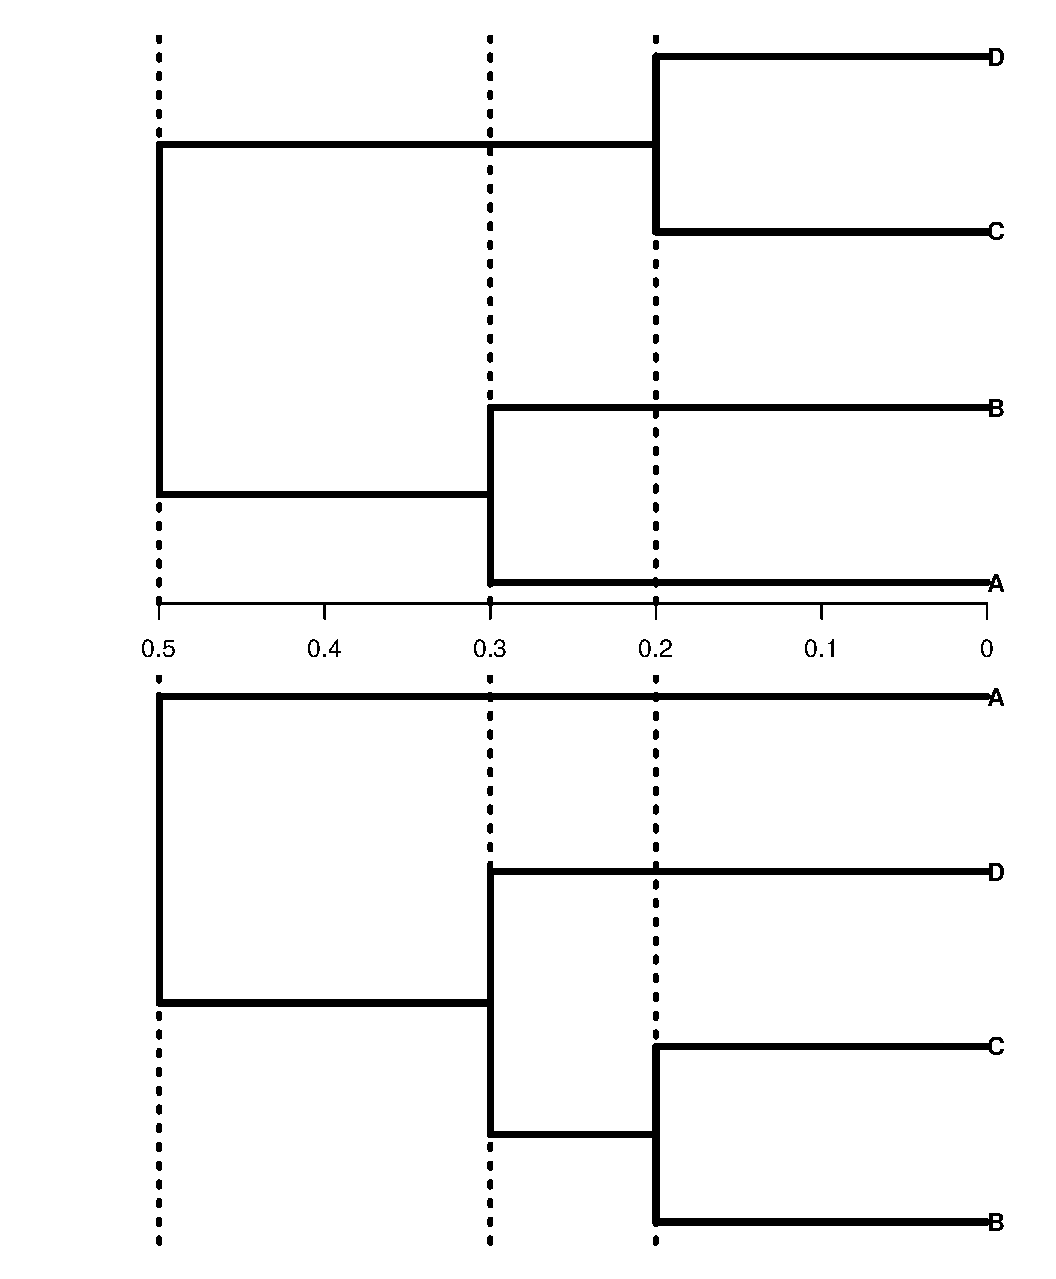
\includegraphics[scale=0.65]{\dir/figs/counter_example_mapping.pdf}
\caption[Two distinct phylogenies with the same intercoalescent intervals and numbers of lineages.]{\textbf{Two distinct phylogenies with the same intercoalescent intervals and numbers of lineages}.
In this example, we would have $\boldsymbol s = \{0.2, 0.1, 0.2\}$ and $\boldsymbol k = \{2, 3, 4\}$.
}
\label{fig:cexample}
\end{figure}

We then conclude that
\begin{remark}
\label{rmk:non_identifiable}
  The parametric prior $\pi_0(\tau| N_e)$ is flat in large portions of $\boldsymbol\Psi$.
\end{remark}
\begin{proof}
Remark~\ref{rmk:InvarCoal} implies that at least one part of the space of interest has the same density under the prior measure for ranked trees (\textit{i.e.} in $\mathbb{T}$).
To see that it remains the case on the space of fully-ranked phylogenies, $\mathbb{F}$, notice that as long as the internal node heights coincide, the phylogenies will have the same density under the prior, since the sampling times ($\boldsymbol a_L$), which are fixed, induce the same sub-intervals~(\cite{Minin2008}, Figure 1.).
% consider the same trees as in Figure~\ref{fig:cexample}, but pay close attention to the terminal branches after the first coalescence event (first dashed line from right to left).
% If all sampling times ($\boldsymbol a_L$) occur before that event, this situation is isomorphic to the contemporaneous case with respect to the summary statistics and by extension the prior measure.
As a consequence, any collection of fully-ranked phylogenies with this configuration would have the same density under the coalescent prior. 
\end{proof}

A statistical consequence of Remark~\ref{rmk:non_identifiable} is that the coalescent prior may fail to regularise any multimodality induced by the likelihood.
In a way, the coalescent prior can be seen as an exchangeable prior on $\boldsymbol \Psi$~\citep{Aldous1996}.
Moreover, this prior is uniform on the space of ranked topologies, but induces counter-intuitive priors on individual clades~\citep{Pickett2005} complicating interpretations of posterior support for clades\footnote{In the interest of fairness, however, it must be said that a uniform distribution over clades is impossible under most prior measures~\citep{Steel2006}.}.
Despite these caveats, the coalescent prior is very common in applications and hence I shall use it as prior measure on $\boldsymbol \Psi$.

\subsection{Theoretical properties of SubtreeJump and SubtreeLeap}
\label{sec:stx_properties}

In this section I explore some of the theoretical properties of the candidate-generating mechanisms described here.

\begin{remark}
\label{rmk:stj_ergodic}
 SubtreeJump does not induce an ergodic Markov chain on $\boldsymbol \Psi$.
 \end{remark}
\begin{proof}
 Since \verb|STJ| does not update branch lengths, the result is obvious.
 However, notice that \verb|STJ| is not irreducible on $\mathbb{F}$ either.
 To see this, consider a phylogeny $\tau^\star = (t^\star, \boldsymbol b^\star) \in \boldsymbol \Psi$ such that for some pair of nodes $i$, $j$  in $t^\star$ such that $j \neq S_i$, either $h(i) < h(P_j)$ or $h(j) < h(P_i)$.
 Then  the move $ i \to j$ is not allowed and hence \verb|STJ| is not irreducible in $\mathbb{F}$.
 The extreme case is when the condition above holds for \textit{every} pair of nodes, resulting in a perfect ladder tree which is an absorbing state the chain can never leave.
\end{proof}

Since~\verb|STL| can change branch lengths, it does not suffer from this limitation.
In particular,
\begin{remark}
\label{rmk:stl_irreducible_F}
 SubTreeLeap induces an irreducible Markov chain on $\mathbb{F}$.
 \end{remark}
\begin{proof}
First, assume $h(i) > 0 \: \forall i \in V_t$ for any phylogeny $\tau \in \boldsymbol \Psi$ with topology $t$.
Recall that $d_{\text{SPR}}(u, x)$ is the number of SPR operations needed to transform $u$ into $x$ (section~\ref{sec:spr_stuff}, Chapter 1).
Define $\mathcal{N}(x) := \{ u \in \mathbb{F} : d_{\text{SPR}}(u, x) = 1 \}$ as the \textit{neighbourhood} of $x \in \mathbb{F}$.
 Ideally, we could show irreducibility if $q_\sigma(y | x) > 0$ for all $\: x, y \in \mathbb{F}$.
 However, we cannot make this claim directly, because $q_\sigma(y | x) > 0$ only for $y \in \mathcal{N}(x)$, which is true because there exists $\: \delta^\star$ such that $P(x \rightarrow y | \delta^\star) > 0 $ and $\kappa(\delta^\star | \sigma) > 0 \: \text{for} \: \delta^\star > 0 \: \text{and} \: \sigma > 0$ by construction.
 Since the SPR graph is connected (see Section~\ref{sec:spr_stuff} in Chapter 1), it follows that any sequence of topologies $\boldsymbol X = \{ X^{(0)}, X^{(1)}, \ldots, X^{(N)}\}$ where $X^{(i + 1)} \in \mathcal{N}( X^{(i)})$ has positive probability under the transition kernel, establishing irreducibility in topological space.
%  (see also Remark~\ref{rmk:stl_K_irreducible}).
\end{proof}

% Let us now derive the induced conditional distributions w.r.t. the prior measure.
% Recall that  the inter-coalescent intervals $\boldsymbol s$ and the numbers of lineages $\boldsymbol k$ (\textit{i.e.} $\psi(\tau)$) are the only quantities of interest, hence we need only to consider the mappings $\omega : \boldsymbol S \to \boldsymbol S$ and $\xi : \boldsymbol K \to \boldsymbol K$ induced by any candidate-generating mechanism.
% Observe that when one has contemporaneous tips and a bifurcating topology, $\boldsymbol k = \boldsymbol k^\prime = \{ n, n-1, \ldots, 3, 2\}$ for any $t \in \mathbb{F}$.
% Under serial sampling the dates of the tips induce extra coalescent subintervals~\citep[Fig. 1]{Minin2008}, so care needs to be taken.
% 
% Consider a phylogeny $\tau$ and the resulting phylogeny after a \verb|STJ| move, $\tau^\prime$.
% Let $(\boldsymbol s, \boldsymbol k) = \psi(\tau)$ and $(\boldsymbol s^\prime, \boldsymbol k^\prime) = \psi(\tau^\prime)$.
% By disconnecting a subtree we reduce the number of lineages by 1, and by reattaching it elsewhere, we break up a branch and increase the number of lineages by 1.
% Since the subtree is reattached at the same height, the ordering (indexing) between the lineages does not change, leading to the conclusion that $\boldsymbol k^\prime = \boldsymbol k$ and hence $\pi_0(\tau) = \pi_0(\tau^\prime)$.
% Also, since \verb|STJ| does not change branch lengths (node heights), $\boldsymbol s = \boldsymbol s^\prime$.
% Therefore, for \verb|STJ| both $\omega$ and $\xi$ are the identity function and, for $\alpha > 0$:
% \begin{equation}
% \label{eq:stj_lineage_kernel}
%   q_1(\boldsymbol k^\prime | \boldsymbol k, \alpha) =
% \begin{cases}
% 1, \boldsymbol k^\prime = \boldsymbol k\\
% 0, \boldsymbol k^\prime \neq \boldsymbol k.
% \end{cases}
% \end{equation}
% Notice also that the marginal kernel $q_1(\boldsymbol k^\prime | \boldsymbol k) = \int_0^\infty q_1(\boldsymbol k^\prime | \boldsymbol k, \beta)d\beta$ is identical to the conditional one because the kernel does not depend on $\alpha$.
% The kernel for the numbers of lineages $q_2(\boldsymbol s^\prime | \boldsymbol s, \alpha)$ is defined analogously to~(\ref{eq:stj_lineage_kernel}).
% 
% The case for \verb|STL| is more complicated.
% % and deriving the transition kernels w.r.t. $\boldsymbol s$ and $\boldsymbol k$ analytically is a daunting task.
% % Here I instead show that \verb|STL| induces irreducible Markov chains on both $\boldsymbol S$ and $\boldsymbol K$,  establishing its irreducibility with regard to the prior.
% As before, let $\tau = (t, \boldsymbol b)$ and $\tau^\prime = (t^\prime, \boldsymbol b^\prime)$ be the state before and after a \verb|STL| operation.
% Recall the move starts by picking a node $i$ uniformly with probability $(2n-2)^{-1}$ and drawing a distance $\delta \sim k(\cdot | \sigma)$ and creating a set $\boldsymbol D_i(\delta^\prime)$, from which a destination $j$ will be picked\footnote{Notice that $\boldsymbol D_i(\delta)$ is a deterministic transform of $\tau$ and $\delta$.}. 
% Special care needs to be taken when extending the tree above the root and I will deal with this case explicitly whenever necessary.

% We need to consider two main cases: (1) a sliding move (SM) where the node $P_i$ moves up or down in height by $\delta^\prime$ -- notice this includes the case $P_i  = \rho$ -- for which  $t = t^\prime$ and; (2) a topology-changing move, equivalent to an SPR operation.
% Let $h^\delta$ be the height at which the pruned subtree subtended by $P_i$ is re-grafted.
% (2) a ``same subtree move'' where $P_i$ is reattached above its current height but within the same subtree or (3) an ``across the root'' move, where $\delta^\prime$ is large enough to warrant destinations above the current root and across the root on the other side of the tree (see Figure~\ref{fig:stl} in Chapter 2).
% Cases (2) and (3) result in a topology-changing move, while case (1), 
% It is convenient to see \verb|STL| as an SPR move, more specifically, conditional on a distance $\delta^\prime$, \verb|STL| is an operation on a restricted neighbourhood $\mathcal{N}_{\delta^\prime}(x)$; when topology does not change -- case (1) -- therefore $\mathcal{N}_{\delta^\prime}(x)$ needs to be modified slightly.
% 
% Let us first study the kernel for the numbers of lineages $q^\sigma_1 : \boldsymbol K \to \mathbb{R}^+$.
% Since $\boldsymbol k$ is intimately related to the topology $t$, one can use the behaviour and properties of \verb|STL| on $\mathbb{T}$ (or $\mathbb{F}$) to gain insight.
% Consider the case where topology does not change: $\boldsymbol k^\prime = \boldsymbol k$ with probability.
% When $t^\prime \neq t$ deriving the exact kernel (specially the marginal kernel w.r.t the distance) is hard because the mapping $\xi$ is a very complicated function that depends on the shape of $t$ as well as the sampling structure $\boldsymbol a_L$.
% I claim that
% \begin{remark}
% \label{rmk:stl_K_irreducible}
% \verb|STL| is irreducible on $\boldsymbol K$,~\textit{i.e.}, $q^\sigma_1(\boldsymbol k^\prime | \boldsymbol k) = \int_0^\infty q_1(\boldsymbol k^\prime | \boldsymbol k, \delta)\kappa(\delta | \sigma)d\delta > 0,\: \forall  \: \boldsymbol k, \boldsymbol k^\prime \in \boldsymbol K$.
% \end{remark}
% \begin{proof}
%  The argument is similar to that in Theorem~\ref{thm:stl_ergodic} and I will not repeat it here.
%  I highlight the fact that the mapping $\mathbb{F} \to \boldsymbol K$ is surjective non-injective and hence irreducibility on topological space implies irreducibility on the space of lineages.
%  Remark~\ref{rmk:k_kprime} takes care of extending the results from the contemporaneous case to the serially-sampled one.
% \end{proof}
% 
% We now turn attention to the inter-coalescent intervals $\boldsymbol s$.
% When $P_i = \rho$, $s^\prime_2 = s_2 \pm \delta^\prime$ and $s^\prime_i = s_i\: \forall \: i > 2$.
% This establishes the mapping $\omega$ for this case -- notice $\omega^{-1}$ exists.
% It is convenient to observe that each node $e$ in $\tau$ is unambiguously associated\footnote{The mapping $u : [1, 2, \ldots, 2n-2] \to [2, 3, \ldots, N_z]$ is bijective.
%  I am however glossing over the fact that node numberings change slightly from $\tau$ to $\tau^\prime$ in case of a topological rearrangement, but this should not pose any unsurmountable difficulty.} with an inter-coalescent interval $s_{u(e)}$, defined by two node heights such that $s_{u(e)} =  h^a_{u(e)} - h^b_{u(e)}$.
% When a topological re-arrangement happens, the interval corresponding to $P_i$ merges with its neighbour: $s^\prime_{u(i)} = s_{u(i)} + s_{u(i) + 1}$.
% In addition, reattaching the pruned subtree at $P_j$ with height $h^\prime(\delta) = 2\text{mrca}_{ij}-h(P_i)-\delta$ splits an interval $s_{u(j)}$ in two: $s_{u(j)}^\prime = h^a_{u(j)} - h^\prime(\delta)$ and $s_{u(j) + 1}^\prime = h^\prime(\delta) - h^b_{u(j)}$.
% % Using a known fact about patristic distances and the fact that these distances can be written as functions of node heights, we arrive at 
% We are then finally prepared to write $s^\prime = \omega(\boldsymbol s, \delta)$: 
% \begin{align}
%  \label{eq:coalescent_ints_mapping}
% %   \boldsymbol  & = \\
%   =\begin{cases}
% s_2^\prime = s_2 \pm \delta, \: s^\prime_i = s_i\: \forall \: i > 2, \text{if}\: P_i = \rho; \\
% s_2^\prime = s_2 + \delta - h(\rho) + h(P_i), \: s^\prime_i = s_i\: \forall \: i > 2,\:\text{if}\: j = \rho \: \text{and}\: \delta > h(\rho) - h(P_i);\\
% s_{u(i)}^\prime = s_{u(i)} \pm \delta, s_{u(i) + 1}^\prime = s_{u(i) + 1} \pm \delta \: \text{with} \: s^\prime_i = s_i\: \forall \: i \neq u \neq u + 1, \text{if SM};\\
% s_{u(i)}^\prime =  s_u(i) + s_{u(i) + 1},\: s_{u(j)}^\prime = h^a_{u(j)} - h^\prime(\delta)\: \text{and} \: s_{u(j) + 1}^\prime = h^\prime(\delta) - h^b_{u(j)}\:\text{if SSTM or CTM}. 
% \end{cases}
% \end{align}
% Although the inter-coalescent intervals are a complicated function of the the distance $\delta$, all functional forms are linear. 
% Notice also that the cases that involve the root node follow the same pattern and thus do not pose any extra difficulties.

\begin{theorem}
\label{thm:stl_ergodic}
 SubTreeLeap induces an ergodic Markov chain on $\boldsymbol\Psi$ with respect to $p$. % LM: probably false....
\end{theorem}
\begin{proof}
 I will show that \verb|STL| is irreducible and aperiodic, which establishes ergodicity~\citep{Meyn1993,Roberts2004,Dinh2017}.
 First, we need to show irreducibility on $\boldsymbol\Psi$ by extending the result of Remark~\ref{rmk:stl_irreducible_F} to include branch lengths.
 Suppose there exist $\tau, \tau^\star \in \boldsymbol\Psi$ such that $\tau^\star$ cannot be reached from $\tau$ in finitely many \verb|STL| steps.
 Following Remark~\ref{rmk:stl_irreducible_F}, we may, withouth loss of generality, assume they have the same topology,~\textit{i.e.} $t = t^\star$, and that differences between the two phylogenies lie solely in their branch lengths.
 This would imply that there exist two phylogenies with the same topology that cannot be transformed into one another in finitely many sliding moves, which is clearly false.
 Note that \verb|STL| has a positive probability of producing a sliding move for any node it picks and all nodes (excluding the root) can be picked for any given \verb|STL| operation.
 
 Now let us show that \verb|STL| is aperiodic.
 Recall that $\tau  = (t, \boldsymbol b)$ and let $r_\sigma(\tau)$ be the probability that $t = t^\prime$ -- conditional on $\boldsymbol b$ -- and let $A = \{x : r_\sigma(x) > 0\}$.
 The chain is aperiodic on $\mathbb{F}$ because $ p(A) > 0 \: \forall \: A \subset \boldsymbol \Psi$ and $r_\sigma(\tau) > 0 \: \forall \: \tau $  -- according to~\cite{Tierney1994} (pg. 1705) this result can be found in Section 2.4 of~\cite{Nummelin1984}.

 Aperiodicity with respect to branch lengths can be shown using a similar argument to the one used above for irreducibility.
 We will use the concept of Harris recurrence~\citep{Harris1956,Chan1994,Tierney1994}.
 First, denote the $n$-th state of the chain by $X^{(n)}$ and define $\kappa_A = \sup \{ n \geq 1 : X^{(n)} \in A \} $ for $A \subset \boldsymbol \Psi$.
 Following the definitions and results in~\cite{Roberts2006}, for our purposes it suffices to show that $\text{Pr}(\kappa_A < \infty | X^{(0)} = x) = 1$ for all $x \in \boldsymbol \Phi$ -- since we know that $p(A) > 0$ for all $A$.
 Again making use of Remark~\ref{rmk:stl_irreducible_F}, we may restrict attention to a family of (sub)sets $A_t = \{x : d_{\text{SPR}}(x, t) = 0 \}$ for some $t \in \mathbb{F}$.
 Now one can use reasoning by contradiction similarly to what was done above to deduce that $\text{Pr}(\kappa_{A_t} = \infty | X^{(0)} = x) = 0$ for $x \in \boldsymbol \Phi$ and for all $t$.
 If $d_{\text{SPR}}(x, t) = 0$ we use the sliding move argument above, otherwise we employ Remark~\ref{rmk:stl_irreducible_F} to get us to the case where it is.
 These arguments establish Harris recurrence of the chain induced by \verb|STL| with respect to branch lengths, completing the proof.
\end{proof}
This establishes the suitability of \verb|STL| for use as the sole phylogenetic transition kernel in a MCMC analysis.

\begin{remark}
 \verb|STL| induces a lazy random walk on the SPR graph.
\end{remark}
Since $d_\text{SPR}(\tau, \tau^\prime)$ is either $0$ or $1$, it follows that the projection of a \verb|STL| random walk on the SPR graph $G_n$ is a random walk that moves to a neighbouring state with probability $1- m_\delta$ and stays put with probability $m_\delta$, \textit{i.e.},  an $m_\delta-$lazy random walk.
We can compute $m_\delta$ from the set of heights $\boldsymbol H(\tau)$ and a fixed distance $\delta$ by realising that for an \verb|STL| move to \textit{not} result in a topological change, we need to pick a node $i$ such that only a sliding move (SM) is possible.
I claim we can write $m_{\delta}$ as follows
\begin{align}
 m_{\delta} &:= P(d_\text{SPR}(\tau, \tau^\prime) = 0) \propto  \sum_{j \in V_t} P( \text{SM} | j,  \delta), \\
  & = \frac{1}{2n-2} \left( 1 + \frac{\mathbb{I}(p_L > \delta) + \mathbb{I}(p_R > \delta)}{2} + \right. \\
  & \left. \sum_{i \in \boldsymbol R(\tau)} \left[ 1 \wedge \left(  \frac{1}{2}\left \{ \mathbb{I}(q_i > \delta) \times \mathbb{I}(p_i >  \delta)  \right \} + \mathbb{I}( g_i > \delta) \right) \right] \right),
\end{align}
where $p_i $, $q_i$  and $g_i$ are as before and $\boldsymbol R(t)$ is the set of all nodes of $t$ excluding the root and its two children, $L$ and $R$.
Notice $m_\delta = 1$ when $\delta < \min( \boldsymbol B(\tau))$ and $m_\delta = 1/ (2n-2)$ when $\delta  > \max( \boldsymbol B(\tau))$.
It is important however to point out that $m_\delta$ depends on $\tau$ -- and as such should really be written as $m^\tau_{\delta}$ -- which makes the lazy random walk probability state-dependent.

\subsection*{Correctness}
\label{sec:correctness}

As illustrated in~\cite{Holder2005}, who show an error in the Hastings ratio of a popular phylogenetic transition kernel, implementing valid MCMC samplers for phylogenetics can be tricky.
Incorrect transition kernels can lead to wrong inferences by converging to the wrong target (posterior) distribution or not converging at all.
Since phylogenetic space is non-standard, it poses special difficulties to ascertaining the correctness of MCMC implementations, due to its sheer size and the difficulty in obtaining analytical results against which samples can be compared.
While some authors opt for two independent  implementations, usually in different programming languages -- e.g.~\cite{Drummond2002} and~\cite{Dinh2017} -- others choose to validate their samplers by comparing results with other known samplers or theoretical results~\citep{Hoehna2008}.
In this chapter I shall take the latter approach, which I describe in more detail below.

Specifically in the case of phylogenetics, we need to ascertain whether both topologies and branch lengths are sampled correctly.
Suppose MCMC is used to approximate the posterior probabilities $P_i = p(T_i | \boldsymbol D),\: i = 1, 2, \ldots, F_n$.
If $\boldsymbol X = \{X^{(0)}, X^{(1)}, \ldots, X^{(M)}\}$ is a Markov chain where each $X^{(j)}$ is a phylogeny sampled at the $j$-th state, one can approximate $P_i$ as:
\begin{equation}
 \label{eq:treeFreq}
 P_i =  \frac{1}{M}\sum_{j=0} ^M \mathbb{I}(X^{(j)}, T_i),
\end{equation}
where $\mathbb{I}(Y, T_i)$ is an indicator function that is $1$ if $Y$ and $T_i$ have the same topology\footnote{One can say, for instance, that if the rSPR distance between two trees $A$ and $B$ is $0$, then $A = B$.} and $0$ otherwise.
Branch lengths will be dealt with in a different way (see below).
Of course, the bigger $S(n)$, the larger $M$ will have to be in order to obtain good estimates.
Since our goal is to assess correctness, it will be convenient to assume that the only parameter of interest is the phylogeny $\tau$~\citep{Lakner2008}.

\subsubsection{Comparison with samples from the prior}
As a baseline for assessing correctness of a transition kernel, one should determine whether its induced Markov chain can accurately sample from the prior.
There are several aspects of a MCMC sample that can be analysed with respect to their theoretical  expectations of both their continuous and discrete components.
% I compared clade and tree frequencies obtained with the default MCMC scheme for very long (golden) runs also compared the distribution of inter-coalescent intervals with their theoretical counterparts using goodness-of-fit tests.
% The results seem to indicate that our candidate-generating mechanisms lead to transition kernels with the correct limiting distribution.

First, we would be interested in determining whether our kernel allows accurately sampling from the -- discrete projection of -- prior distribution $\boldsymbol R = \{R_1, R_2, \ldots, R_{S(n)} \}$ of trees (topologies).
In practice, a good estimate of $\boldsymbol R$ can be obtained by simulating a large number $K$ of phylogenies from the coalescent prior distribution and calculating the true tree probabilities as described in equation~(\ref{eq:treeFreq}).
To assess correctness, in particular, one can sample then run MCMC for a suitably large number $M$ of iterations, calculate empirical frequencies $\boldsymbol F = \{F_1, F_2, \ldots, F_{S(n)} \}$ in the same fashion and then compare $\boldsymbol F$ and $\boldsymbol R$.
If the sampler is correct, these distributions should match each other very closely.
One can define an error measure $\Delta$
\[ \Delta := \max_{1 \leq i \leq S(n)} \frac{|F_i - R_i|}{R_i}, \]
usually called the \textit{maximum relative deviation}.  

As the dimensionality of the posterior distribution grows, it becomes progressively harder to accurately sample the distribution of trees, even in the absence of data.
Hence, an approach routinely used in practice is look at the distribution of clades instead.
Recall that for $n \geq 3$ taxa there are $ A(n) = |\boldsymbol C| = 2^{n-1} -1$ possible clades. 
As $n \rightarrow \infty$, $A(n)/F(n) \rightarrow 0$, making tracking clades instead of trees an attractive alternative when dealing with larger data sets commonly encountered in practice ($n$ in the lower hundreds).

Comparing clade distributions can be done analogously to comparing tree (topology) distributions  -- as exemplified in Section~\ref{sec:cladeSwitch} Chapter 3, the probabilities under the prior can be computed exactly.
In particular one can define a similar error measure~\citep{Hoehna2008}:
\[ \delta := \max_{1 \leq i \leq A(n)} \frac{|F^c_i - R^c_i|}{R^c_i}, \]
where $\boldsymbol F^c$ and $\boldsymbol R^c$ are the true (theoretical) and observed probabilities as before.

\subsubsection{Coalescent times}

In addition to looking at topologies, we also need to ensure the distribution of branch lengths is being accurately sampled.
To this end, we can look at the distribution of coalescent intervals.
Under a constant population size ($N_e$) coalescent model, the $k-$th coalescent interval is distributed according to an exponential($\lambda_k$), where $\lambda_k = \frac{k(k-1)}{4N_e}$, $k = 1, 2, ..., n-1$.
With this in hand, one can then analyse a sample of trees and assess whether the empirical (observed) distribution of coalescent times matches the theoretical distribution.
For instance, one can perform a goodness-of-fit test to ascertain whether the distribution sampled~\textit{via} MCMC adheres to its theoretical counterpart.

\subsubsection{Dealing with data: marginal likelihoods}

\cite{Hoehna2008} propose another approach to obtain posterior probabilities, which is to calculate marginal likelihoods for every tree topology.
Under the assumption that $\boldsymbol D$ was generated by a model $M(\boldsymbol \theta)$, where $\boldsymbol \theta$ is a parameter vector, the marginal likelihood for tree $T_i$ is
\begin{align}
 \label{eq:margLike}
 l_i = p(\boldsymbol D | T_i) = & \int_{\boldsymbol \Theta} p(\boldsymbol D | T_i, \boldsymbol \theta) \pi(\boldsymbol \theta | T_i)d\boldsymbol \theta. 
\end{align}
The claim by \cite{Hoehna2008} is that $\frac{l_i}{l_j} = \frac{P_i}{P_j} \quad \forall i, j \in \{1, 2, \ldots, S(n)\}$.

However, this only holds when a uniform prior probability distribution on trees is assumed. 
When different topologies have different prior probabilities, one must multiply the ratio $l_i/l_j$ by $\pi(T_i)/\pi(T_j)$ before comparing ratios.
Here I will present results in log space to reduce numerical instability.

I simulated an alignment with $L = 40$ sites using a five taxa phylogeny (contemporaneous tips) under a simple HKY model with $\Gamma$-distributed site-rate heterogeneity ($\alpha = 0.05$).
I then ran BEAST for $1$ billion iterations, producing a sample of $1$ million trees.
Marginal likelihoods were calculated by running BEAST with each tree fixed and computing the marginal likelihood using the generalised stepping stone (GSS) method described in~\cite{Baele2015}.
For GSS I used $100$ steps with 1 million iterations each ($\beta = 0.3$).

\subsubsection{Correctness results}
\label{sec:correctness}

Figure~\ref{fig:treeP} shows that all tested kernels are able to approximate the true distribution within $5\%$ absolute error, whilst Figure~\ref{fig:cladeP} shows that clade frequencies could be estimated below $1\%$ absolute error for all kernels.
These results suggest that the moves proposed here correctly lead to the target the distribution of interest in terms of tree topologies and clades.
An attentive reader will notice we plot $5\%$ bands for the tree comparisons and $1\%$ bands for the clade comparisons. 
This is because estimation for clade probabilities is much more precise then for tree probabilities.
These thresholds are inherently arbitrary and I feel $5\%$ is an acceptable threshold.
I draw attention to the fact that the error measures discussed here are \textbf{relative}, whereas other authors have chosen absolute error loss functions~\citep{Hoehna2008, Lakner2008}.
In practice this means our thresholds are more strict than previously adopted.

Next, I look at the estimates of the coalescent intervals.
As shown in Figure~\ref{fig:coalIntervals}, all tested kernels seem to produce correct approximations to the distribution of coalescent times.
Whilst I could do formal goodness-of-fit tests on the obtained distribution against the theoretical distributions, it often suffices to visually inspect the histogram of coalescent times and check the proximity of the central moments.%TODO: maybe actually run the goodness of fit stuff

The last set of analyses pertains to the behaviour of the transition kernels when targeting the \underline{posterior} distribution.
As suggested by~\cite{Hoehna2008}, the frequency of a particular tree in the posterior sample should be proportional to its marginal likelihood.
Figure~\ref{fig:logP} shows the the plot of $\log P_i$ against $\log l_i$ for both the default mix and STL, colouring points by their \verb|rspr| distance to the true tree.
In Figure~\ref{fig:ratios} I plot log posterior probabilities against corrected marginal likelihoods for every pair $i, j$ such that $i < j$\footnote{Since the ratio correspondence is symmetrical, it suffices to look at the lower triangular entries in the full comparison matrix.}.
I confirm the claim by~\cite{Hoehna2008}, adding, however, that direct comparison between $l_i$ and $P_i$ is only possible when assuming a uniform distribution on topologies.
In our example, the coalescent prior does \textbf{not} assign equal probability across topologies\footnote{Note that the coalescent prior places a uniform distribution over~\textit{labelled histories}.} and thus one needs to account for the prior probabilities $\boldsymbol R$ in order to obtain a linear relationship between the posterior frequency of a tree and its marginal likelihood.

One thing to note is that, even on  a log scale, there seems to be a small bias in the results presented in Figure~\ref{fig:ratios}, whereby for small marginal likelihood ratios (i.e., more similar trees) there seems to be an overestimation of the ratio of posterior probabilities and conversely for bigger marginal likelihood ratios we see some underestimation.
This might be due to instability in the denominator, a common pitfall of ratio estimation.
Also, the estimates obtained with SubTreeLeap also seem to be more noisy, although it remains to be seen whether these differences are relevant.
Overall, I believe it is possible to claim that both SubTreeJump and SubTreeLeap are correct and target the correct (posterior) distribution.

% \subsubsection{Possible extensions}
% 
% The checking procedures discussed here have been applied only to contemporaneous sequences.
% Therefore, an obvious extension would be to consider the correctness of tree kernels when dealing with temporally-sampled (heterochronous) tips.
% 
% An interesting idea, perhaps unrelated to correctness assessment, is to vary the alignment size $L$ and determine for which $L_0$ the true tree used to generate the data has both the highest marginal likelihood and highest posterior probability (for various $n$).
% This would give us some insight into the informational content of the data under simple models and inform about how much one can actually learn from the data.

\begin{figure}[!ht]
\centering
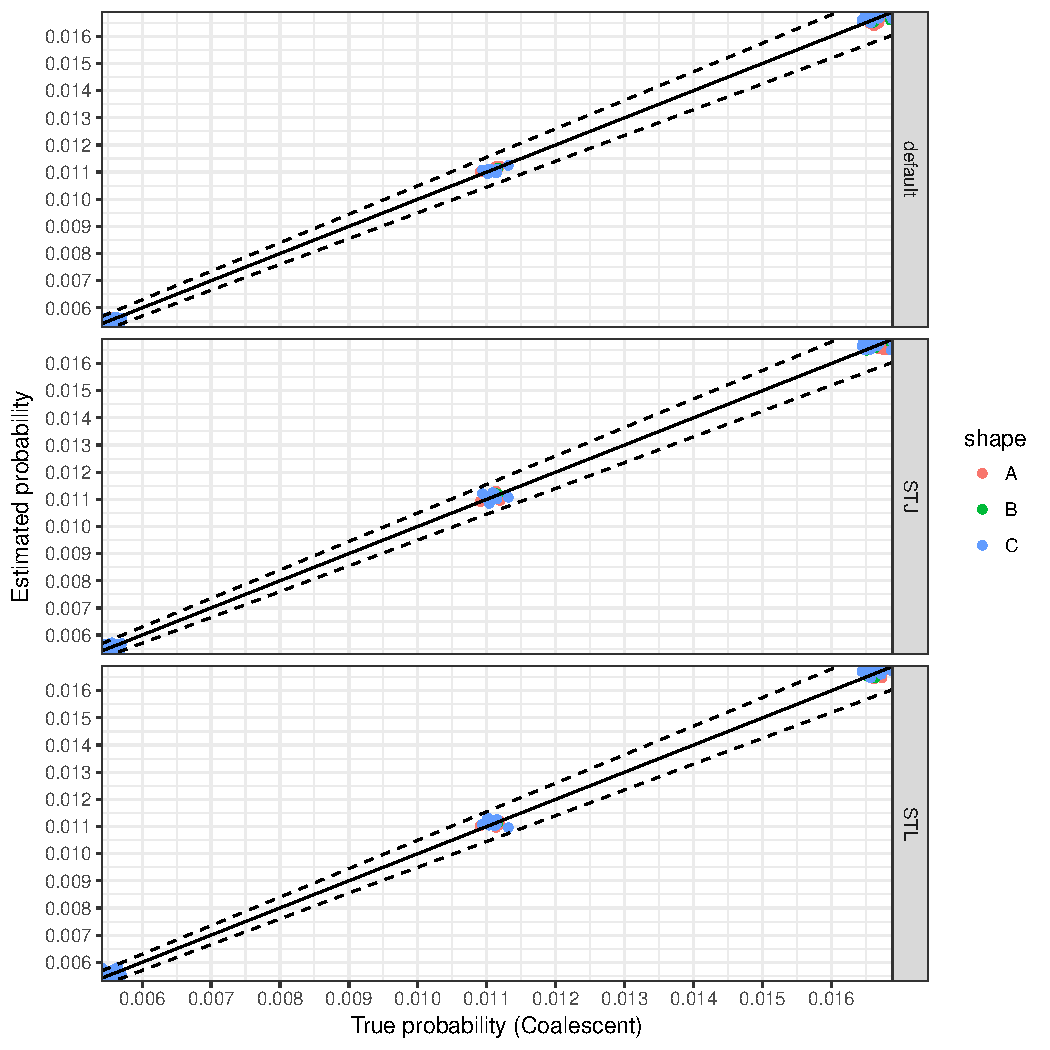
\includegraphics[scale=0.75]{\dir/figs/TreeProbabilities_5taxa.pdf}
\caption[Tree probabilities obtained by sampling from the prior with each transition kernel.]{\textbf{Tree probabilities obtained by sampling from the prior with each transition kernel}.
For each tree kernel, we present the estimated probabilities for each of the $105$ possible trees on $5$ taxa from a sample of $M = 1, 000, 000$  trees.
On the x-axis, we present the true probabilities, computed from a sample of $K = 100, 000$ trees from the coalescent prior by direct simulation.
For comparison, probabilities estimated using the default mix of kernels in BEAST v.1.8.4 are provided in the top panel.
Solid line shows $x=y$ and the dashed lines show $5\%$ limits.
Colours show the three possible tree shapes for $5$ taxa.
}
\label{fig:treeP}
\end{figure}
%%%
\begin{figure}[!ht]
\centering
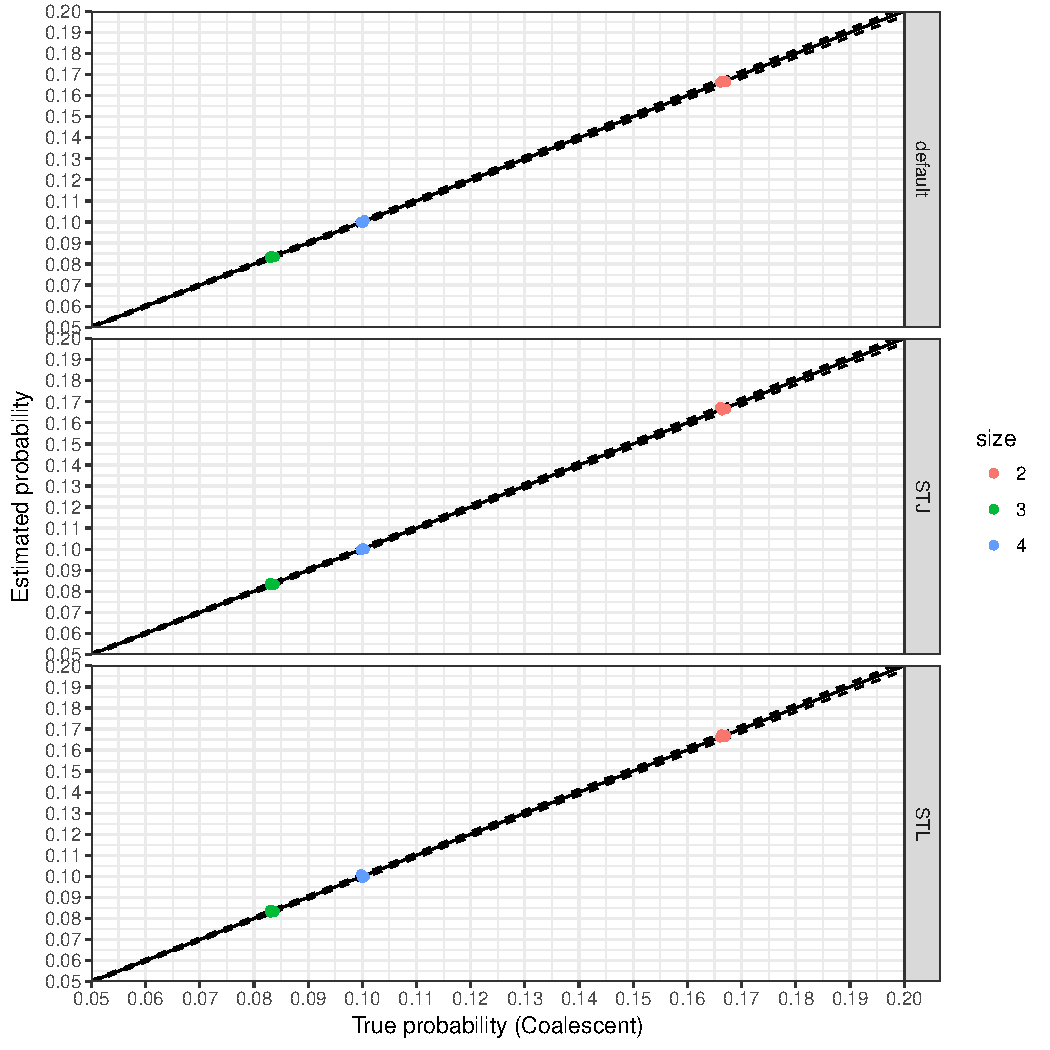
\includegraphics[scale=0.75]{\dir/figs/CladeFrequencies_5taxa.pdf}
\caption[Clade probabilities obtained by sampling from the prior with each transition kernel.]{\textbf{Clade probabilities obtained by sampling from the prior with each transition kernel}.
I used the same sample of $1$ million trees to compute clade frequencies to compute the clade frequencies.
On the x-axis, I present the true clade probabilities, computed from a the same sample from the prior as before.
Probabilities estimated using the default mix of kernels in BEAST v.1.8.4 are again provided in the top panel.
Solid line shows $x=y$ and the dashed lines show $1\%$ limits.
Colours show the three possible clade sizes for $5$ taxa (excluding singletons and the set of all leaves/tips).
}
\label{fig:cladeP}
\end{figure}
%%%
\begin{figure}
\begin{center}
  \subfigure[\textbf{Coalescent simulation}]{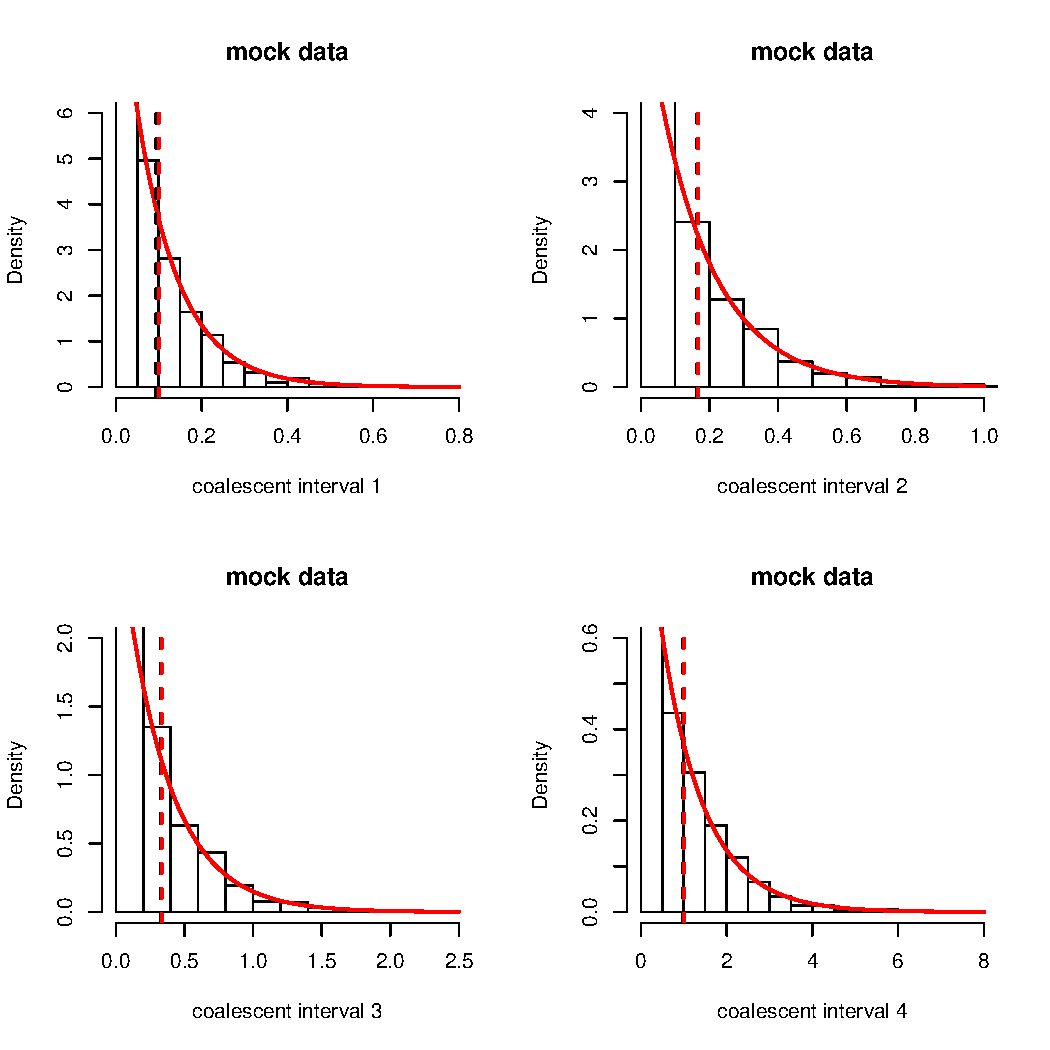
\includegraphics[scale=0.4]{\dir/figs/coalInts_coalSim.pdf}}%
  \subfigure[\textbf{Default operators}]{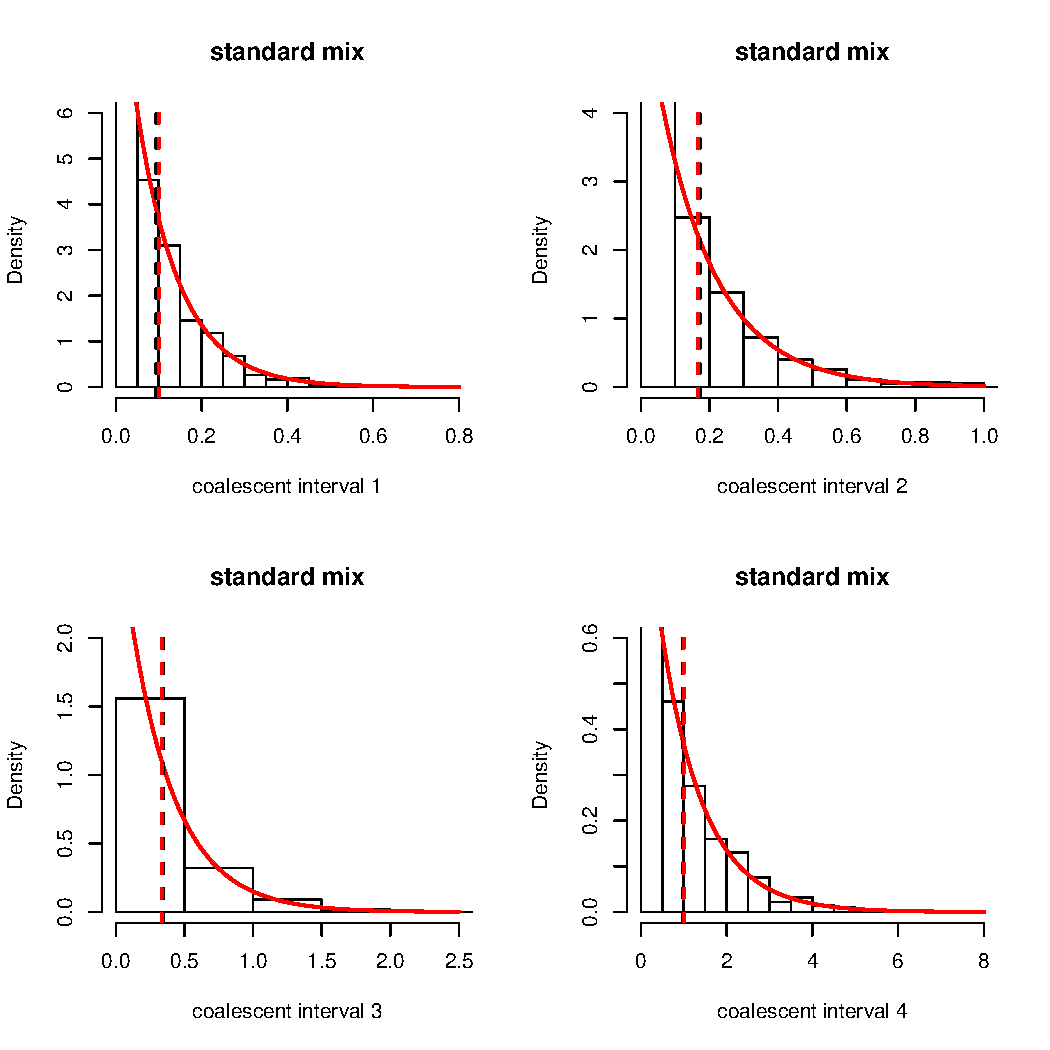
\includegraphics[scale=0.4]{\dir/figs/coalInts_standard_mix.pdf}}  
  \subfigure[\textbf{SubTreeJump}]{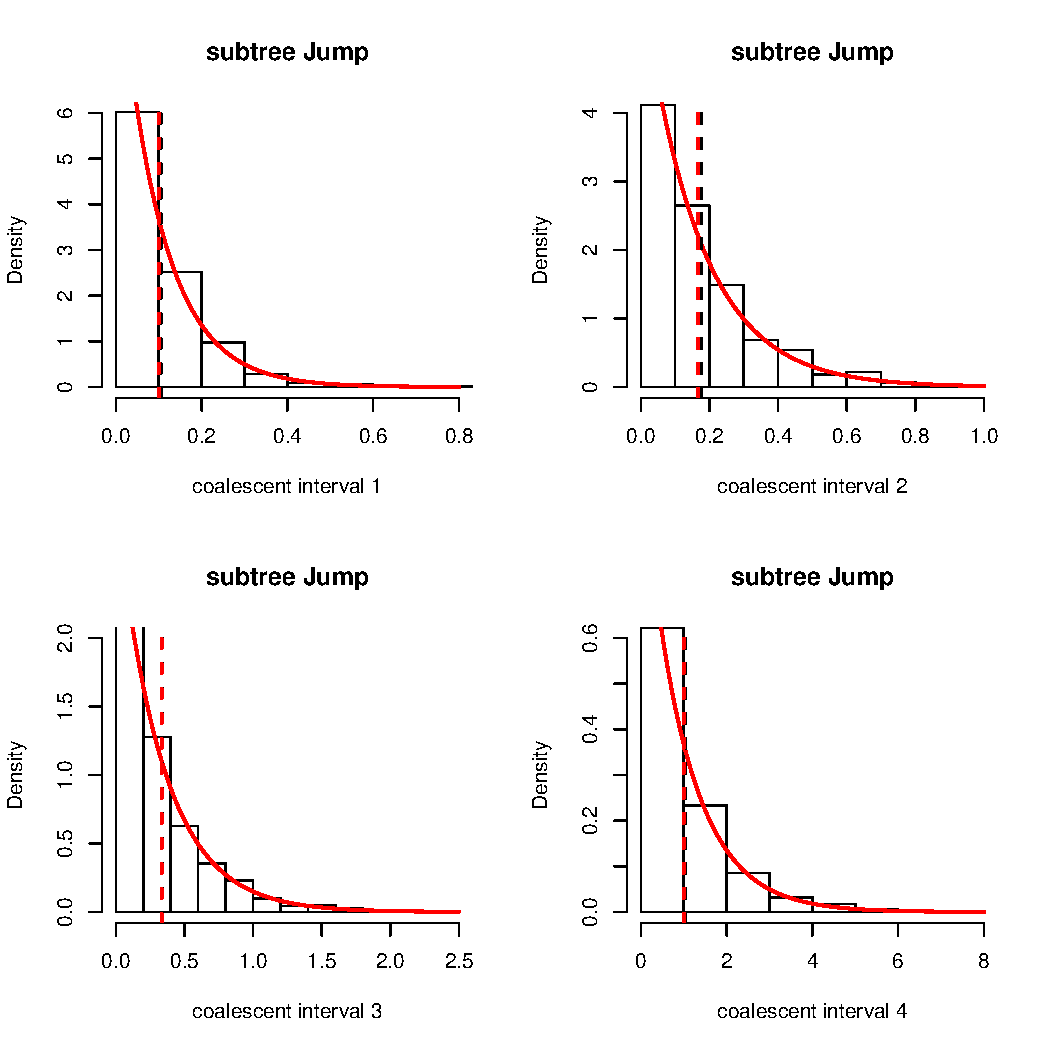
\includegraphics[scale=0.4]{\dir/figs/coalInts_SubTreeJump.pdf}}%
  \subfigure[\textbf{SubTreeLeap}]{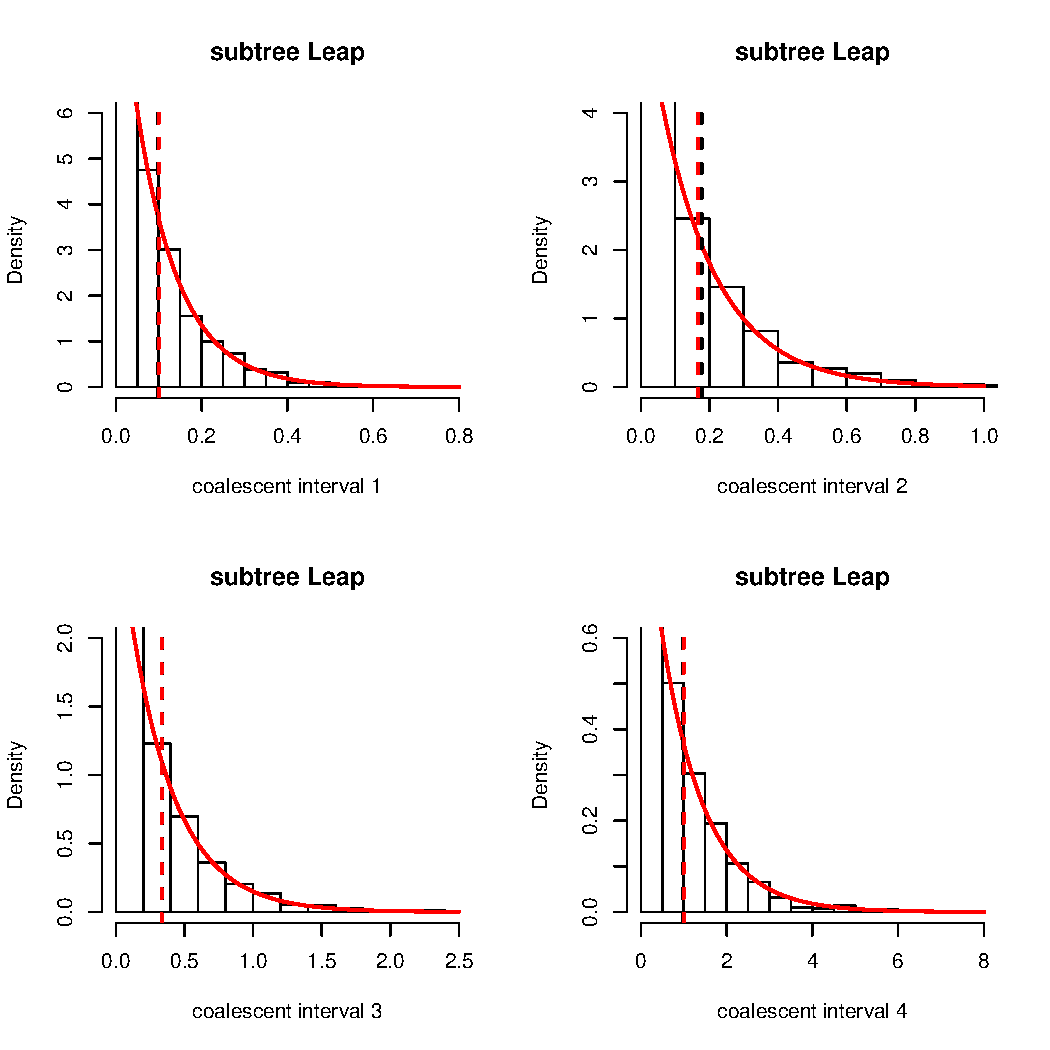
\includegraphics[scale=0.4]{\dir/figs/coalInts_SubTreeLeap.pdf}}
\end{center}
\caption[Coalescent interval distributions obtained by direct simulation, the default (standard) mix of operators in BEAST and our two new kernels.]{\textbf{Coalescent interval distributions obtained by direct simulation, the default (standard) mix of operators in BEAST and our two new kernels}.
I show the distributions of the four coalescent intervals for $n = 5$ and $N_e = 1000$  obtained by (a) direct simulation from the coalescent process, (b) sampling with the default mix of operators (kernels), (c) SubTreeJump and (d) SubTreeLeap.
Red and black vertical dashed lines show the theoretical and estimated means, respectively, and the solid red line shows the theoretical density. 
To be able to sample with SubTreeJump, we need to combine it with branch length transition kernels, whilst SubTreeLeap can sample on its own.}
\label{fig:coalIntervals}
\end{figure}
%%%
\begin{figure}[!ht]
\centering
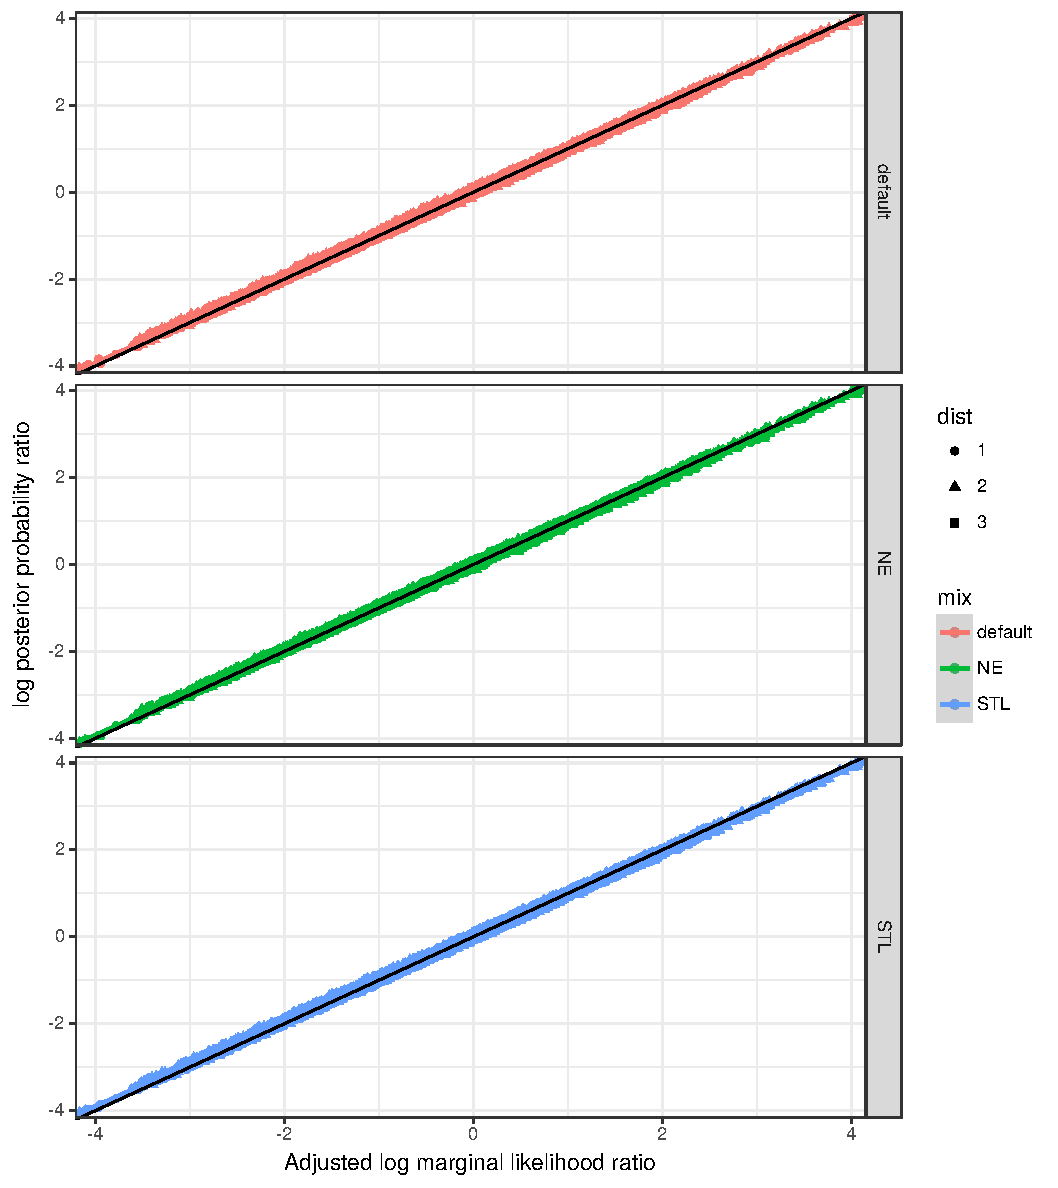
\includegraphics[scale=0.75]{\dir/figs/NE_ratioP_vs_ratioMargLike_40L_1Biter.pdf}
\caption[Log posterior probabilities versus marginal (log) likelihoods.]{\textbf{Log posterior probabilities versus marginal (log) likelihoods}.
I plot $\log P_i - \log P_j$ against $(\log l_i - \log l_j) + (\log \pi(T_i) - \log\pi(T_j))$ for the default mix and SubTreeLeap.
Points are coloured according to their rspr distance to the true tree.
Notice that distance zero means the true tree, used to be simulate the data.
}
\label{fig:logP}
\end{figure}
%%%
%%% 
\begin{figure}[!ht]
\centering
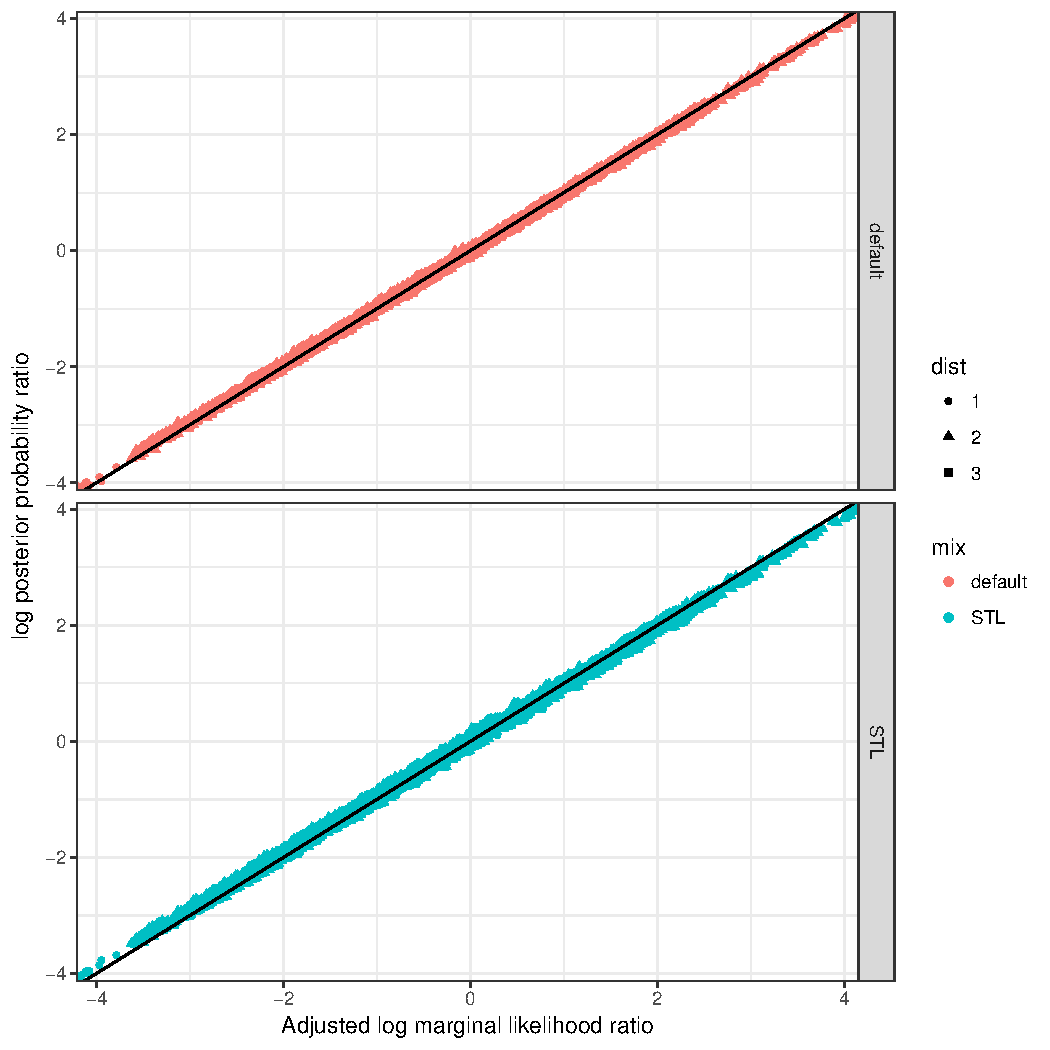
\includegraphics[scale=0.75]{\dir/figs/ratioP_vs_ratioMargLike_40L_1Biter.pdf}
\caption[Ratios of posterior probabilities of the trees against the ratio of their marginal likelihoods.]{\textbf{Ratios of posterior probabilities of the trees against the ratio of their marginal likelihoods.}
In this figure I show the (log) ratios as proposed by~\cite{Hoehna2008}.
All computations as in Figure~\ref{fig:logP}.
Solid black line shows $x = y$.
Point shapes depict the distance between the pair of trees.
}
\label{fig:ratios}
\end{figure}  

\section{Data}

\subsection{Real-world data sets}
\label{sec:realworld}

I compiled a collection of serially-sampled data sets of fast-evolving RNA viruses of various sizes -- in terms of number of taxa/sequences and  alignment length-- in order to have challenging real-world data sets to test the new kernels on (Table~\ref{tab:datasets}).

Data sets \verb|Dengue4|, \verb|RSVA| and \verb|YFV| are widely used in phylodynamics as teaching data sets and have been extensively analysed.
These data sets also have moderate numbers of sequences, which permit better exploration of available methods by allowing more -- and longer -- chains to be run.
To assess performance in bigger, more realistic data sets I composed three more collections of RNA virus sequence alignments, described below.

To compose \verb|denv2Genome|, I downloaded  $2382$ full genomes (aligned) from Broad Institute's Dengue Virus Portal (\url{http://www.broadinstitute.org/annotation/viral/Dengue/}), filtered those from serotype 2 and then subsampled to have at most five samples from each year.
This resulted in a data set consisting of $90$ full genome from DENV-2 isolates from the Americas, ranging from 1987 to 2007.
\verb|denv2Env| was constructed by selecting only the envelope sequence for each of the full genomes.
Sequences were downloaded pre-aligned.

\verb|flu| is comprised of Human Influenza H3N2 hemagglutinin (HA) sequences ($\approx 1700$ bp).
I downloaded all human HA sequences with more than $1700$ base pairs from the Influenza Research Database~(\url{http://www.fludb.org/brc/home.spg?decorator=influenza}), totalling $8455$ sequences, with sampling dates ranging from $1969$ to $2014$. 
To make analyses feasible, I downsampled by including at most five sequences from each subsequent year were randomly sampled, resulting in a final data set comprised $225$ sequences, which were then aligned by codons using the Geneious software package~(\url{http://www.geneious.com/}).

I downloaded all HIV subtype B polymerase (pol) gene sequences from the Los Alamos HIV sequence database~(\url{http://www.hiv.lanl.gov/content/sequence/HIV/mainpage.html}) and retained those with known sampling year.
This data set comprised $2523$ sequences, with sampling years in the period $1983-2013$.
Downsampling was carried out in the same fashion of that for Influenza by keeping the $39$ unique sequences from $1983$ and sampling from subsequent years, resulting in $187$ sequences in the final data set (\verb|HIV|)\footnote{The sequences were downloaded pre-aligned and the final alignment was manually checked for inconsistencies.}.

Finally,~\verb|EBOVa| is one of the largest phylodynamic data sets assembled to date, composed of 1610 serially-sampled full genome sequences of Ebola virus, curated by~\cite{Dudas2017}.
In order to speed up computations without losing realism, I consider a modified version of the data set without the intergenic regions (\verb|EBOVb|).
I spend a considerable portion of this chapter discussing ways of improving MCMC performance for data sets \verb|EBOVa| and \verb|EBOVb|, since they represent the type of challenging data set that is quickly becoming the norm in phylodynamics.

\begin{sidewaystable}[!ht]
\caption[Collection of serially-sampled data sets.]{\textbf{Collection of serially-sampled data sets used in this study.}
I report the number of taxa, nucleotide sites and time span (maximum - minimum) of the sequence dates.
Denv2 has two versions, one where the alignment consists of full genomes  (a) and one with only the \textit{env} gene (b).
All data sets were DNA sequence alignments.
DENV = Dengue fever virus; RSV = Respiratory Syncytial Virus; YFV = Yellow fever virus; HIV = Human immunodeficiency virus; EBOV = Ebola virus (Makona).
}
\begin{center}
\begin{tabular}{cccccccc}
\toprule
Data set & Type of data	& \# sequences & \# sites & span (years) & Reference \\             
\midrule
Dengue4 & DENV serotype 4 \textit{env} gene& 17  & 1485 & 38 & \cite{Lanciotti1997}\\
RSVA & RSV subgroup A \textit{G} protein & 35 & 629 & 46& \cite{Zlateva2004}\\
YFV & YFV~\textit{prM/E} gene & 71  & 654 & 69 & \cite{Bryant2007}\\
denv2Env/denv2Genome & DENV serotype 2 full genome/\textit{env} gene & 90  & 11851/1441 & 45 & this study\\
HIV & HIV~\textit{pol} gene & 187 & 3012 & 30 & this study\\
flu & Influenza virus H3N2 HA gene & 225  & 1705 & 45 & this study\\
EBOVa/b & EBOV full genome & 1610 & 18992/14518 & 1.6 &~\cite{Dudas2017} \\
\bottomrule
\end{tabular}
\end{center}
 \label{tab:datasets}
\end{sidewaystable}

\section{Computational details}
\label{sec:compdetails}

At each iteration BEAST picks a transition kernel (operator) at random from the set of transition kernels, with probability $w_i/\sum_i w_i$, where $w_i$ is called the~\textbf{weight} of operator.
An~\textbf{operator mix} thus is a collection of transition kernels with a certain vector of weights $\boldsymbol w$.
For the experiments presented in this chapter I have constructed five MCMC schemes employing different candidate-generating mechanisms (operators), described in detail in Table~\ref{tab:operator_mixes}.
I compared the default suite of operators in BEAST~\citep{Drummond2012} to schemes containing \verb|FNPR|,~\verb|STJ|,~\verb|STL| and a combination of~\verb|STJ| and \verb|STL|, which I dubbed~\verb|STX|.
The idea behind combining~\verb|STJ| and \verb|STL| was to help the chain make bigger jumps occasionally, since for $\alpha \geq 0$~\verb|STJ| can lead to bold proposals and hence help with mode-jumping (see Section~\ref{sec:STJadap} however).
Notice that when employing either~\verb|FNPR| or~\verb|STJ| I needed to also include ways of updating branch lengths, since these operators promote only topology changes.

\begin{sidewaystable}[!ht]
\caption[Operator mixes used in this study.]{\textbf{Operator mixes used in this study}.
Each mix was composed of Operator $i$ with weight ($w_i$).
Notice all operator mix (or MCMC scheme) was adjusted so $\sum_i w_i = 69$ to make them comparable with the default in BEAST.
}
\begin{center}
% \resizebox{\linewidth}{!}{
% \tabcolsep=2pt
\begin{tabular}{ccc}
\toprule
Operator mix &  Components (weight) \\             
\midrule
Classic (\verb|default|) &  \verb|subTreSlide| (15), \verb|NarrowExchange| (3), \verb|WideExchange| (3), \\ &  \verb|wilsonBalding| (3), \verb|rootHeight| (3), \verb|internalNodeHeights| (30) \\
Fixed-height node prune and regraft (\verb|FNPR|) &  \verb|FNPR| (36), \verb|rootHeight| (3), \verb|internalNodeHeights| (30) \\
SubtreeJump  (\verb|STJ|) &  \verb|subTreJump| (36), \verb|rootHeight| (3), \verb|internalNodeHeights| (30)\\
SubtreeLeap (\verb|STL|) &  \verb|subTreLeap| (69)\\
SubtreeLeap and SubtreeJump (\verb|STX|) & \verb|subTreJump| (63), \verb|subTreLeap| (6) \\
\bottomrule
\end{tabular}
% }
\end{center}
 \label{tab:operator_mixes}
\end{sidewaystable}

\subsection{Adaptation scheme}

The efficiency of $\bar{\mu_g}$ as an estimator depends crucially on the proposal-generating distribution $Q_\omega(\cdot, \cdot)$, which in turn depends on the indexing parameter $\omega$.
In general, $\omega$ can be understood as the~\textit{width} of the proposal; if $\omega$ is too small, consecutive states will be highly correlated, and the chain will not mix well.
On the other hand, if $\omega$ is too large, proposed values are likely to have low density under the target and hence get rejected.
Ideally, one would want to set $\omega$ to an optimal value $\omega^\star$ that maximises the efficiency of chain, as measured by, say, the effective sample size (ESS).
In particular, we would like to find $\omega^\star$ such that the acceptance probability $\alpha$ is at its optimal value, $\alpha^\star$.
Theoretical analyses of a host of MCMC algorithms for a broad class of target distributions have shown that $\alpha^\star \approx 0.234$ ($0.44$ for one-dimensional targets) for random walk Metropolis~\citep{Roberts1997,Roberts2001}, $0.574$ for the Metropolis-adjusted Langevin algorithm (MALA)~\citep{Roberts2001} and $0.651$ for Hamiltonian Monte Carlo (HMC)~\citep{Beskos2013}.

It is convenient to represent the accept-reject mechanism as a binary-valued process with probability $\alpha_\omega$.
In particular, we can write~\citep{Andrieu2008}:
$$\bar{\alpha}_\omega := \int_{\mathcal{X} \times \mathcal{X}} \alpha_\omega(x, y)\pi_d(x) q_\omega(x, y) dxdy.$$
Recall that in parallel to the chain $\{Z_i\}$ we have a chain of proposed values $\{Y_i\}$.
We can formulate the problem of finding $\bar{\alpha}_\omega = \alpha^\star$ as an stochastic approximation problem, more specifically, we can can write~\cite[eq. 17]{Andrieu2008}:
$$ h(\omega) := E_\omega[ H(\omega, Z_0, Y_1, Z_1, \ldots) ] = 0,$$
where
$$ H(\omega, Z_0, Y_1, Z_1, \ldots) :=  \min \left[1, \frac{\pi_d(Y_1) q_\omega(Y_1, Z_0)}{\pi_d(Z_0) q_\omega(Z_0, Y_1)} \right] - \alpha^\star.$$
This is the so-called \textbf{coerced} acceptance probability case, which is is implemented in BEAST.
It is equivalent to finding the zeroes of $h(\omega) = \bar{\alpha}_\omega- \alpha^\star$~\citep{Andrieu2008}.

I shall follow~\cite{Garthwaite2016} and assume that the acceptance probability $\bar{\alpha}_\omega$ is a monotonically-decreasing function of the scale parameter.
The Robbin-Monro algorithm~\citep{Robbins1951} is a popular method for solving the zero-finding problem and consists of creating a positive, non-increasing sequence $\{ \omega_i \}$, $\omega_i: \Omega \times \mathcal{X} \to \Omega$ via an update of the form~\cite[eq. 21]{Andrieu2008}
\begin{equation}
 \label{eq:general_size_update}
 \omega_{n + 1} = \omega_n + \gamma_{n + 1}h(\omega),
\end{equation}
subject to the conditions that $\sum_{n = 0}^\infty \gamma_n = \infty$ and $\sum_{n = 0}^\infty \gamma_n^2 < \infty$.
One way to attain this is to choose $\gamma_n = \mathcal{O}(n^{-c})$ for $1/2 < c \leq 1$~\citep{Atchade2005}.
In practice, we need to replace $h(\omega)$ with an estimate, for instance
\begin{align*}
\widehat{h}(\omega) &:=  \widehat{\alpha(\omega)}_n - \alpha^\star, \\
\widehat{\alpha(\omega)}_n &:= \sum_{j = C_0}^n  \alpha_{\omega_j}(Z_j, Y_j),
% \widehat{\alpha(\omega)}_n &:= \sum_{j = C_0}^n 1-\mathbb{I}_{Z_j}(Y_j).
\end{align*}
% $\mathbb{I}_z(y)$ is 1 when $y = z$ and $0$ otherwise 
where $C_0$ is an integer constant chosen so as to avoid transient effects from the initial states of the chain. 
In BEAST, the Robbins-Monro update is of the form\footnote{Notice that in BEAST the acceptance rate estimate is~\textbf{not} smoothed over the chain.}
\begin{equation}
 \label{eq:beast_size_update}
 \omega_{n + 1} = \omega_n + \frac{1}{f(n) + 1} \left( \alpha_{\omega_n}(Z_n, Y_n) - \alpha^\star\right)
\end{equation}
where $f(x) = x$, $f(x) = \log(x)$ or $f(x) = \sqrt{x}$.
By default $f(x) = \log(x)$ and $C_0 =  \left \lfloor{M/100}\right \rfloor$.
Unfortunately, however, it is not clear to me how $f(x) = \log(x)$ could lead to a valid algorithm, since\footnote{Notice also that $\sum_{n = 0}^\infty \left( \frac{1}{\sqrt{n} + 1}\right)^2 = \infty$.} $\sum_{n = 0}^\infty \left( \frac{1}{\log(n) + 1}\right)^2 = \infty$.
In contrast, $\sum_{n = 0}^\infty \left( \frac{1}{n + 1}\right)^2 = \frac{\pi^2}{6}$.

\subsection{Golden runs}
\label{sec:golden_runs}

Since we do not know the true posterior distribution for any of the empirical data sets described in Section~\ref{sec:realworld}, I ran very long chains for each data set in order to obtain what we will call ``golden runs'', which are intended to be a good approximation to the actual target distributions.
To obtain these golden runs I ran three independent chains for $10^9$ iterations using the default kernels (see above).
I extracted the last $5, 000$ phylogenies from each run and (i) obtained a maximum clade credibility (MCC) tree from the resulting $15, 000$ trees and (ii) computed the $2.5 \times 10^6$ pairwise distances between them under various metrics in order to then obtain MDS projections (see Chapter 3).
I will call these the ``true tree'' and ``true posterior'', respectively.
In order to construct target distributions for the empirical data sets I computed the distance from the ``true tree'' for each of the three golden runs, resulting in $300, 000$  samples from each distribution (for each metric).

\subsection{Performance assessment}
\label{sec:performance_methods}

\cite{Lakner2008} were the first to systematically investigate transition kernel efficiency in MCMC for Bayesian phylogenetics.
They investigated the performance of seven kernels on a collection of 10 real-world data sets.
To quantify performance, the authors looked at the percentage of converged runs per tested kernel, using clade frequencies relative to a reference (golden) run as a criterion.
Time to convergence was also used as performance criterion.
Here I will take a similar approach, but with two important distinctions: (a) less reliance on clade frequencies as a convergence criterion and (b) focus on the sampling of continuous parameters that depend on the tree.
This is because (a) as the number of taxa grows, it becomes increasingly burdensome to keep track of clades and reliably estimate their frequencies and (b) my ultimate goal is to develop phylogenetic transition kernels that allow quick traversal of phylogenetic space and (indirectly) facilitate sampling of continuous parameters that depend on the phylogeny and hence for properly accommodating uncertainty.

Since each data set presents different difficulties to the sampler(s), different chain lengths are needed to obtain appropriate samples from the posterior.
For the performance comparisons I ran 100 independent runs for each operator mix, recording 10,000 samples from the posterior distribution of trees.
This was done for \verb|Dengue4| and \verb|denv2Genome| so as to strike a balance between how representative these data sets were of real-world phylodynamic analyses and computational feasibility of running hundreds of chains.
The idea behind this experiment was to explore the performance of the MCMC schemes in more detail, analysing warm-up times and mixing for the two data sets mentioned above.

To study the performance of each our MCMC schemes (operator mixes), I propose to split the problem in two parts: (i) warm-up and (ii) mixing (see Chapter 1 for definitions).
The idea is to study (i) how quickly each operator reaches the typical set and (ii) once in a high probability region, how efficiently sampling is done.
When analysing simulated data, it is also possible to compute the mean squared error (MSE) for continuous parameters and the effective sample size (ESS) of the  distance to true tree (using various metrics) but this possibility will not be explored in the present chapter.
For the analyses of empirical data sets, I used the golden runs as ground truth.

To measure warm-up time, one needs to find the iteration $i$ such that $\delta(\frac{1}{i}\sum_{k=1}^i\theta^{(k)}, \theta) < \epsilon$, for some choice of error function $\delta$ and threshold $\epsilon$.
Here I will consider a few error functions, specially tailored for phylogenetics.
The first error function I propose is the average absolute error in clade frequencies, i.e., the L1 norm between the estimated clade frequencies and their true counterparts -- as determined by golden runs.
For another global measure of convergence, I propose to find the fraction $p_t$ of the chain at which the distance to the true tree enters the 95\% credibility interval of the target as the warm-up time.
The rationale behind this is that the sampled trees will initially be more distant from the true tree and  once the chain reaches stationarity, samples will remain a certain radius $r_d$ away from the true tree with high probability.
This radius,~\textit{i.e.} the size of the typical set, depends on the metric ($d$) used and also on other factors, such as alignment size.
The fraction $p_t$ is a measure of how quickly the chain reaches the typical set.
A univariate measure of performance could then be to take the maximum value of this fraction across metrics -- thus being conservative.

Finally, one can study the warm-up time by considering what fraction $p_w$ the chain one needs to discard in order to achieve maximum ESS\footnote{One can see ESS as a concave function of $p_w$; too small $p_w$ and ESS will be low due to the transient effect of initial iterations (high autocorrelation); too high $p_w$ and one discards too many samples, bounding ESS above.} for the continuous parameters.
This is done as follows: for a given chain, the~\textbf{ optimal warm-up fraction}, $\hat{p_w}$, is the maximum fraction fraction of the chain one needs to discard in order to obtain the maximum ESS for a given parameter, across all parameters of interest.
Here I have chosen the parameters \verb|prior|, \verb|likelihood|, \verb|posterior|, \verb|treeModel.rootHeight|, \verb|treeLength|, \verb|meanRate|, \verb|CP1.kappa|, and  \verb|CP3.alpha| because they represent the type of continuous parameter a practitioner would be interested in estimating.

Measuring performance  in terms of mixing is an even more delicate issue, because there are several and often incompatible metrics that purport to assess MCMC efficiency.
For instance, should one look at wall clock time,\textit{i.e.}, actual time to complete the run, or should we restrict attention to the number of effective samples from the posterior?
Here I shall however gloss over some of the nuances in favour of a more direct approach, with well-defined goals.
I propose to assess mixing in two main ways: by computing effective sample sizes for continuous parameters (see Chapter 3, Section~\ref{sec:continuous}) and quantifying mixing in phylogenetic space by means of (a) ESS of tree metrics and (b) clade switching (Section~\ref{sec:cladeSwitch}).

\subsection{Analysis of the Ebola virus data set}

In order to evaluate the performance of MCMC schemes on a challenging real-world data set, I performed specific analyses on \verb|EBOVa| and \verb|EBOVb|, focusing on a realistic analysis pipeline.
To this end I ran three independent runs of 100 million iterations each with the default mix of operators,~\verb|STL| and~\verb|STX| leading to 9 chains in total.
The complete model specification is described in~\cite{Dudas2017}.
I then analysed the resulting MCMC runs in terms of convergence and mixing, as well as performing multi-dimensional scaling under several metrics (see Chapter 3, Figures~\ref{fig:mds_ebov_RF} and~\ref{fig:mds_ebov_KC}).

\section{Results}

\subsection{Target distributions}
\label{sec:target}

In Figure~\ref{fig:target_golden} I show the distributions of distance to the true tree for data sets \verb|Dengue4|, \verb|RSVA|, \verb|YFV|, \verb|denv2Env| and \verb|denv2Genome|, obtained using golden runs (see Section~\ref{sec:golden_runs}).
Even in this univariate setting the target distribution can be multimodal and generally non-standard, for most metrics considered.
Discrete metrics such as the RF show multiples peaks as expected, since RF for instance can only take values in $\boldsymbol D_{\text{RF}} = \{0, 1, \ldots, 2(n-3) \} \in \mathbb{N} $.
In Figure~\ref{fig:target_golden}A I show that these distributions however look well-behaved, resembling Poisson distributions~\citep{Bryant2009}.
The distributions for~\verb|denv2Env| and \verb|denv2Genome| seem to be translated versions of one another, with the target for \verb|denv2Genome| having lower variance as expected under regularity conditions (more data, less uncertainty about the central tree). 
Interestingly, the targets for KC metric\footnote{see Chapter 3 for definitions of this and other metrics.} with $\lambda = 0$ (Figure~\ref{fig:target_golden}B)  which reflect topological differences only display very different behaviour, displaying at the same time less granularity and multimodality.
While being somewhat obvious, this result does in fact suggest that multiple metrics, even when designed to capture the same features -- in this case differences in tree topology -- can lead to radically different results (see discussion in Chapter 3 for more).

As expected, focusing on continuous distance metrics that take both topology and branch lengths into account reveals distributions that resemble strictly positive continuous targets encountered routinely in Statistics (e.g. the log-normal distribution).
The Steel-Penny (SP) metric seems to lead to target distributions that more closely resemble univariate continuous target distributions; it is unimodal and smooth, albeit with considerable skewness.
Notable exceptions are the distributions of SP distances for~\verb|denv2Genome|, which presents some clearly defined minor modes (Figure~\ref{fig:target_golden}C, lower left subpanel) and the distributions under the CD metric, shown in~Figure~\ref{fig:target_golden}D.
This is interesting  because the resulting target for a subset of \verb|denv2Genome|, namely \verb|denv2Env|, does not display these features, providing evidence that multimodality may be strongly data set specific -- hence manifesting in some data sets or subsets thereof but not others.
The same pattern of the full data set presenting more modes than a subset can be seen in the lower left subpanel of Figure~\ref{fig:target_golden}B, which shows results under the KC metric with $\lambda = 0$  (topology differences only).
Distributions of the rooted branch distance (BS) to the true tree show comparable levels of smoothness (Figure~\ref{fig:target_golden}E).
In the following sections I will use these target distributions to evaluate the empirical performance of various MCMC schemes (see Section~\ref{sec:performance_methods} for methods).

\begin{figure}[!ht]
\begin{center}
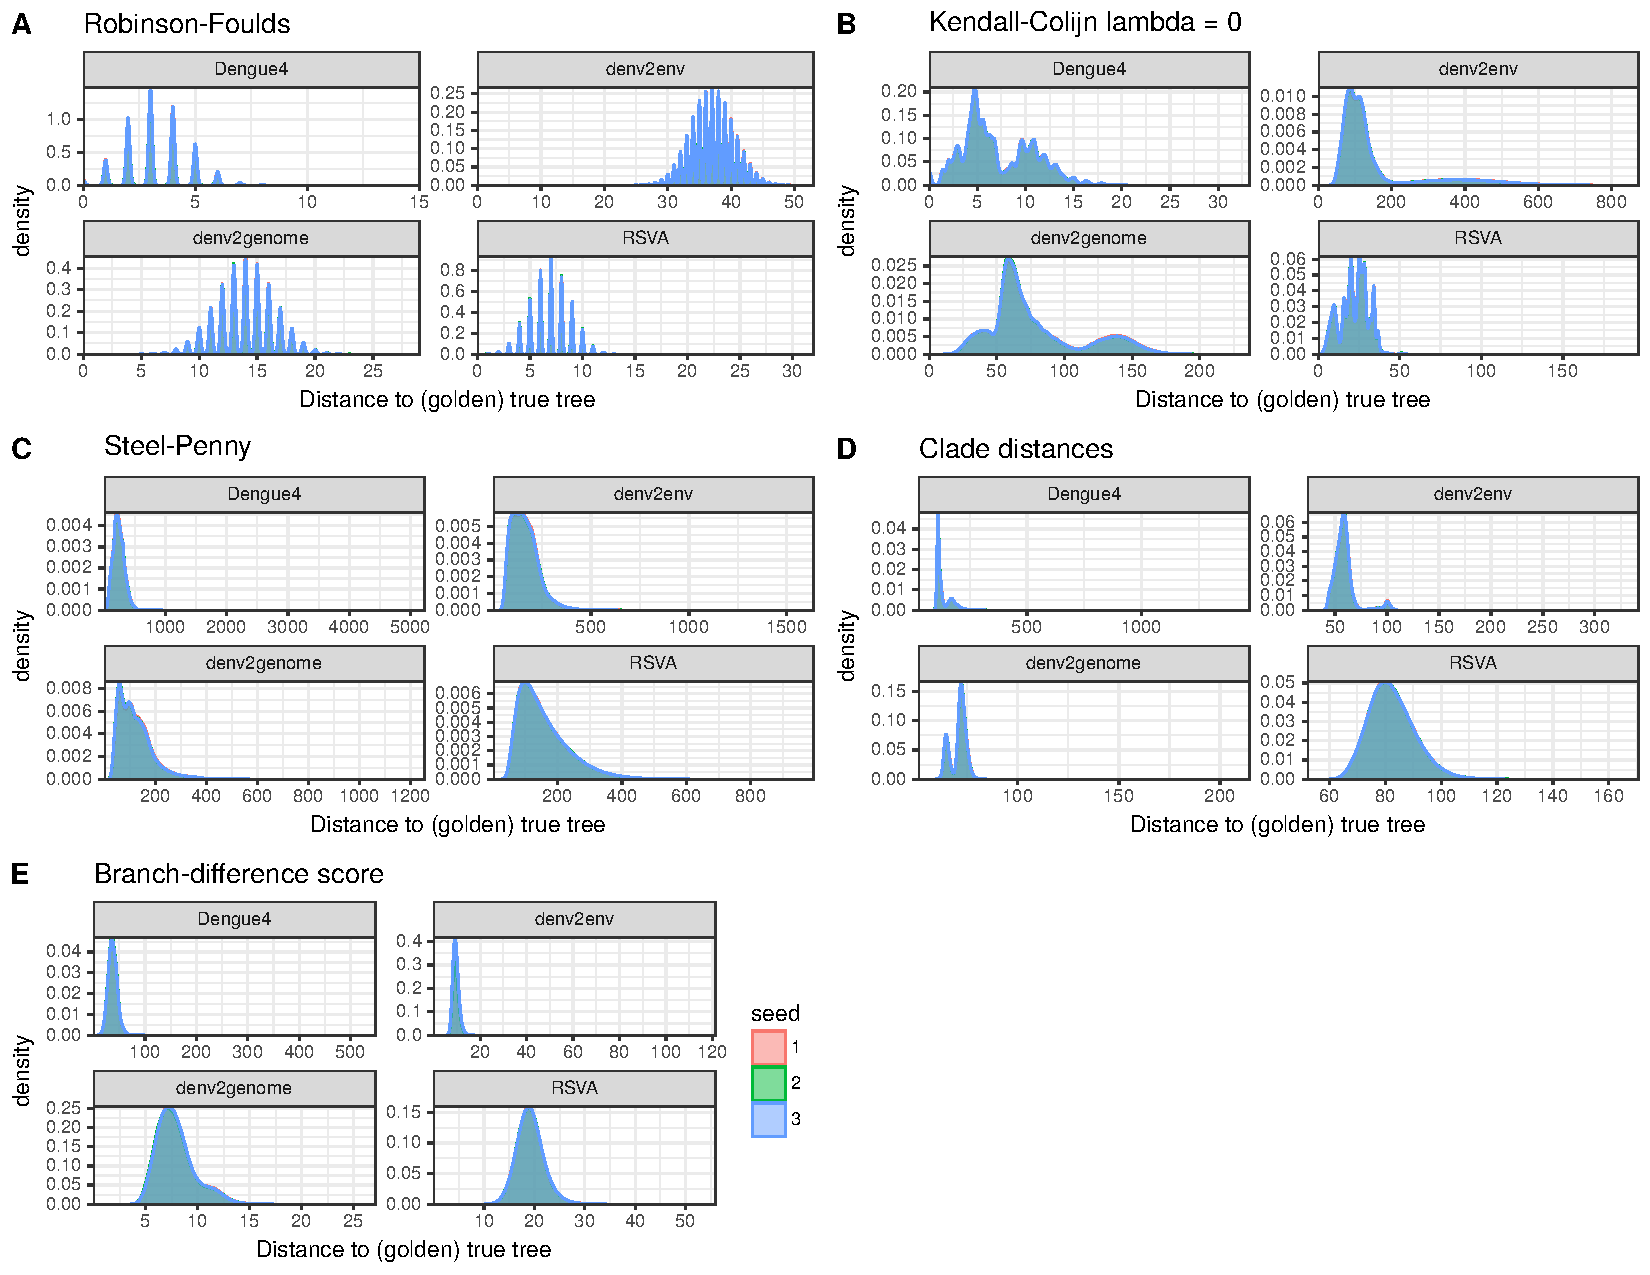
\includegraphics[scale=0.55]{\dir/figs/golden_targets.pdf} 
\end{center}
 \caption[Distance to true golden true tree for several data sets and distance metrics (targets).]{\textbf{Distance to true golden true tree for several data sets and distance metrics (targets).}
 In Panels A and B I show distances that account only for topology differences (\cite{Robinson1981} and~\cite{Kendall2016} (KC) with $\lambda = 0$), whereas panels C, D and E display the distributions of metrics that take branch lengths into account, in the form of the Steel-Penny~\citep{Steel1993}, clade distance (CD) and rooted branch score (BS), see Chapter 3 for definitions.
 Colours show the random generating seed (starting value).
 All kernel density estimates obtained from $100, 000$ samples per starting seed (\textit{i.e.} $300, 000$ samples in total per data set/metric).
 }
 \label{fig:target_golden}
\end{figure}

\subsection{Multimodality in the Ebola 1610 taxa data set}
\label{sec:multimod}

As the results above suggest,a common characteristic of complex discrete-space posterior distributions, particularly Bayesian phylogenetics, is combinatorial multimodality, i.e., multiple peaks composed of atoms (trees) of virtually equivalent posterior density/likelihood separated by valleys of low probability~\citep{Lakner2008,Whidden2015}.
In the middle panel of Figure~\ref{fig:ebovmultimod} it is possible to see that one of the \verb|STL| chains (run 3) gets stuck at a lower density region, which it never leaves.
Run 2 (green line) eventually finds the higher density region and samples from it, whereas Run 1 reaches this mode from the start.
Also from Figure~\ref{fig:ebovmultimod} we can see that neither the default set of operators nor \verb|STX| seem to have any problems reaching the higher density region.
In particular, \verb|STX| seems to quickly find the typical set -- or, more conservatively, the higher mode -- and sample from it, while the default kernels take far more iterations to reach the same region.
Differences between these modes seem to stem from different topologies being explored, as evidenced by the multi-dimensional scaling (MDS) analysis of the Robinson-Foulds metric (see Figure~\ref{fig:mds_ebov_RF} in Chapter 3).
Since SubTreeLeap is a an adaptive kernel, the fact that a particular run got stuck at a lower mode could be due to premature tuning of the scaling parameter to a small value, that would in turn make it nearly impossible for the chain to transition to a higher mode.  
Interestingly however, the SubTreeLeap tuning parameter ($\sigma$) was similar across all three runs shown in Figure~\ref{fig:ebovmultimod}, with run 1 -- which reaches the higher mode from the start -- had $\sigma = 0.116$, while runs 2 and 3 tuned to $0.089$ and $0.087$.

\begin{figure}[!ht]
\begin{center}
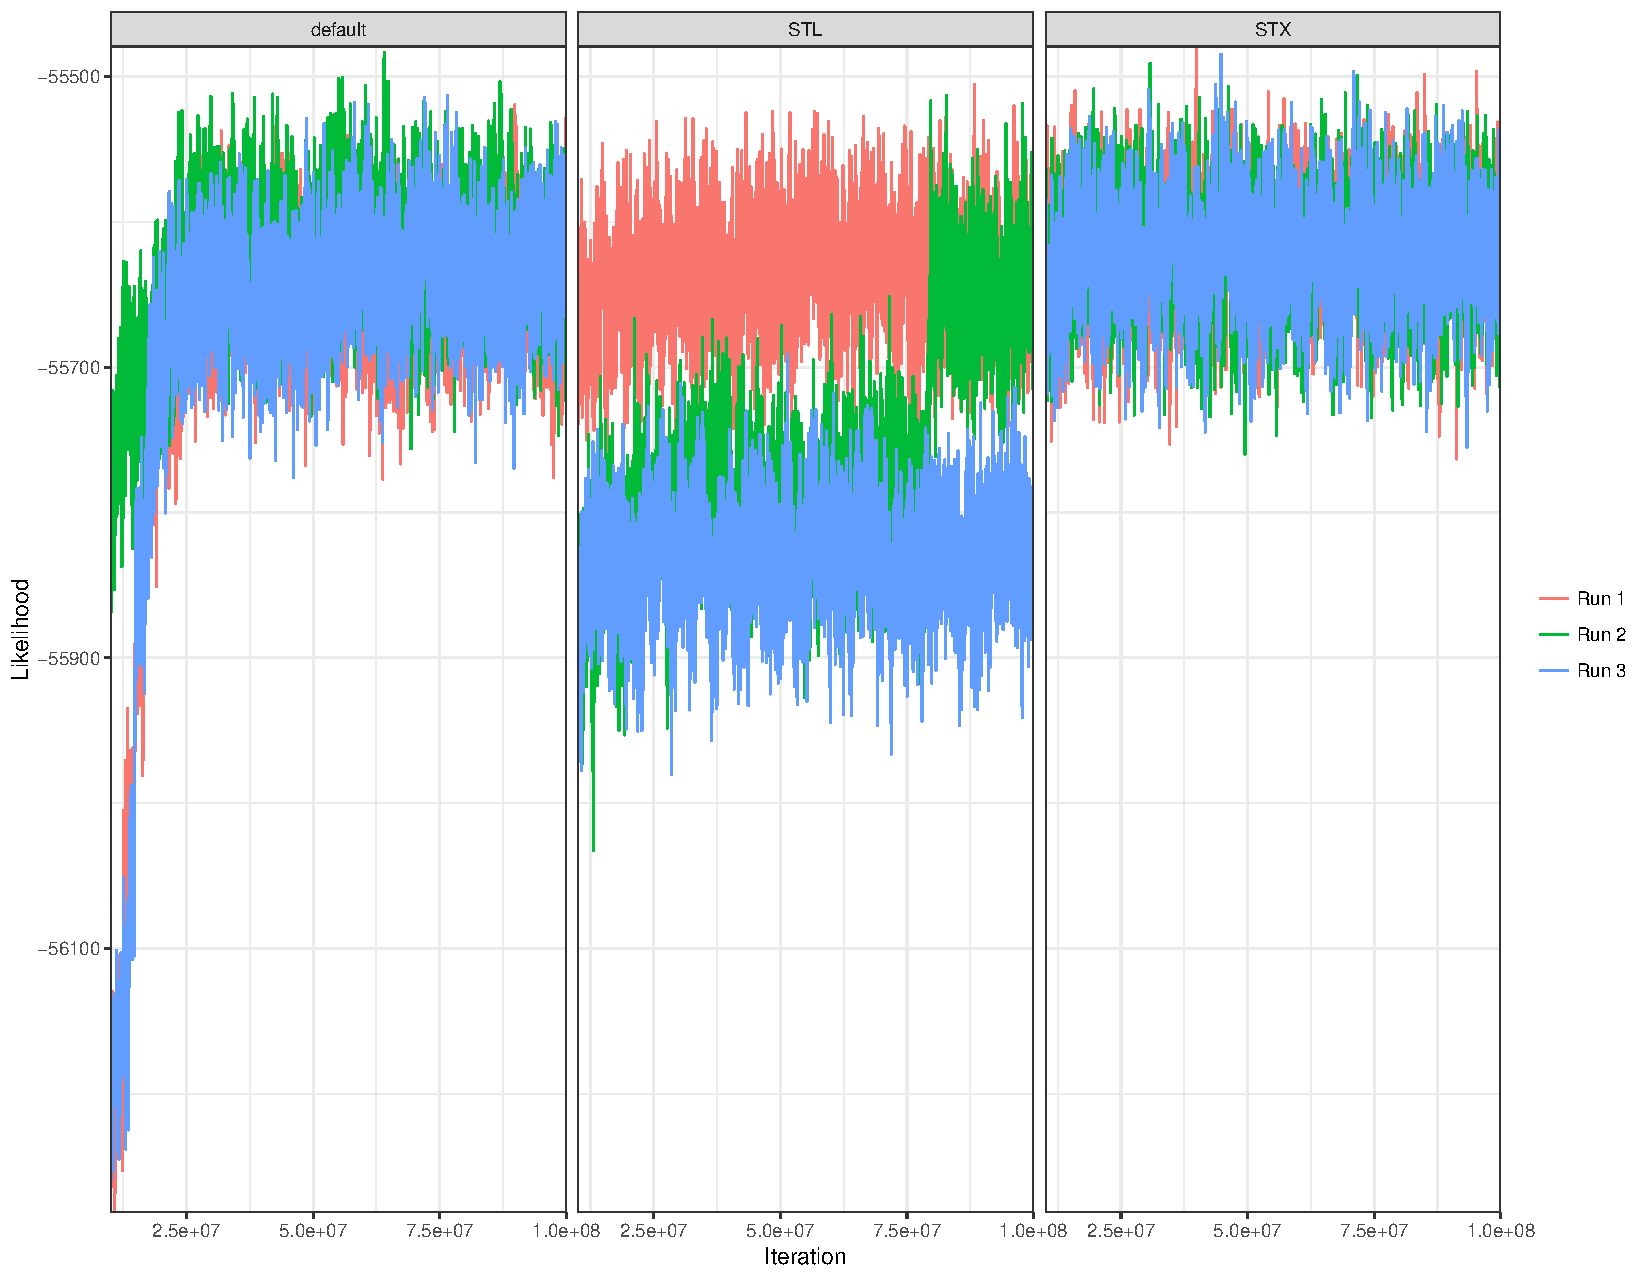
\includegraphics[scale=0.5]{\dir/figs/multi_modes_EBOV.pdf} 
\end{center}
 \caption[Trace plots of the likelihood for the full EBOV 1610 taxa data set.]{\textbf{Trace plots of the likelihood for the full EBOV 1610 taxa data set.}
 I show the traceplots after 10\% of the iterations have been discarded.
 Colours relate to the seed used in the pseudo random number generator, ensuring each run starts from the same point. 
 These computations were performed with the full data set, EBOVa.
 }
 \label{fig:ebovmultimod}
\end{figure}

\subsection{Warm-up, mixing and efficiency}
\label{sec:mcmc_efficiency}

In this section I will discuss the warm-up (burn-in) time, mixing and efficiency of various MCMC schemes considered in this chapter (see Table~\ref{tab:operator_mixes}).
The first quantity I analysed was the fraction $p_t$ of the chain needed to reach the 95\% CI of the target distribution, for various metrics (as shown in Figure~\ref{fig:target_golden}).
These are shown in Figure~\ref{fig:fractions_metrics}.
The first thing to notice is that for most MCMC schemes (operator mixes), only relatively few iterations, under $1\%$ of the total chain length, are required for the chain to start sampling from the bulk of the target distribution.
\verb|STL| and \verb|STX| showed more difficulty reaching the typical set when compared to the default set of operators.
These results are consistent across the two data sets analysed, but the differences in performance are less pronounced for the bigger data set, DENV-2 (90 taxa).
Combining \verb|STJ| and \verb|STL| into \verb|STX| improves warm-up quite substantially, even though it does not outperform the default operators.
This is in tune with the results for the Ebola 1610 taxa data set, for which~\verb|STX| showed faster convergence compared to \verb|STL| (see extended discussion).
\begin{figure}[!ht]
\begin{center}
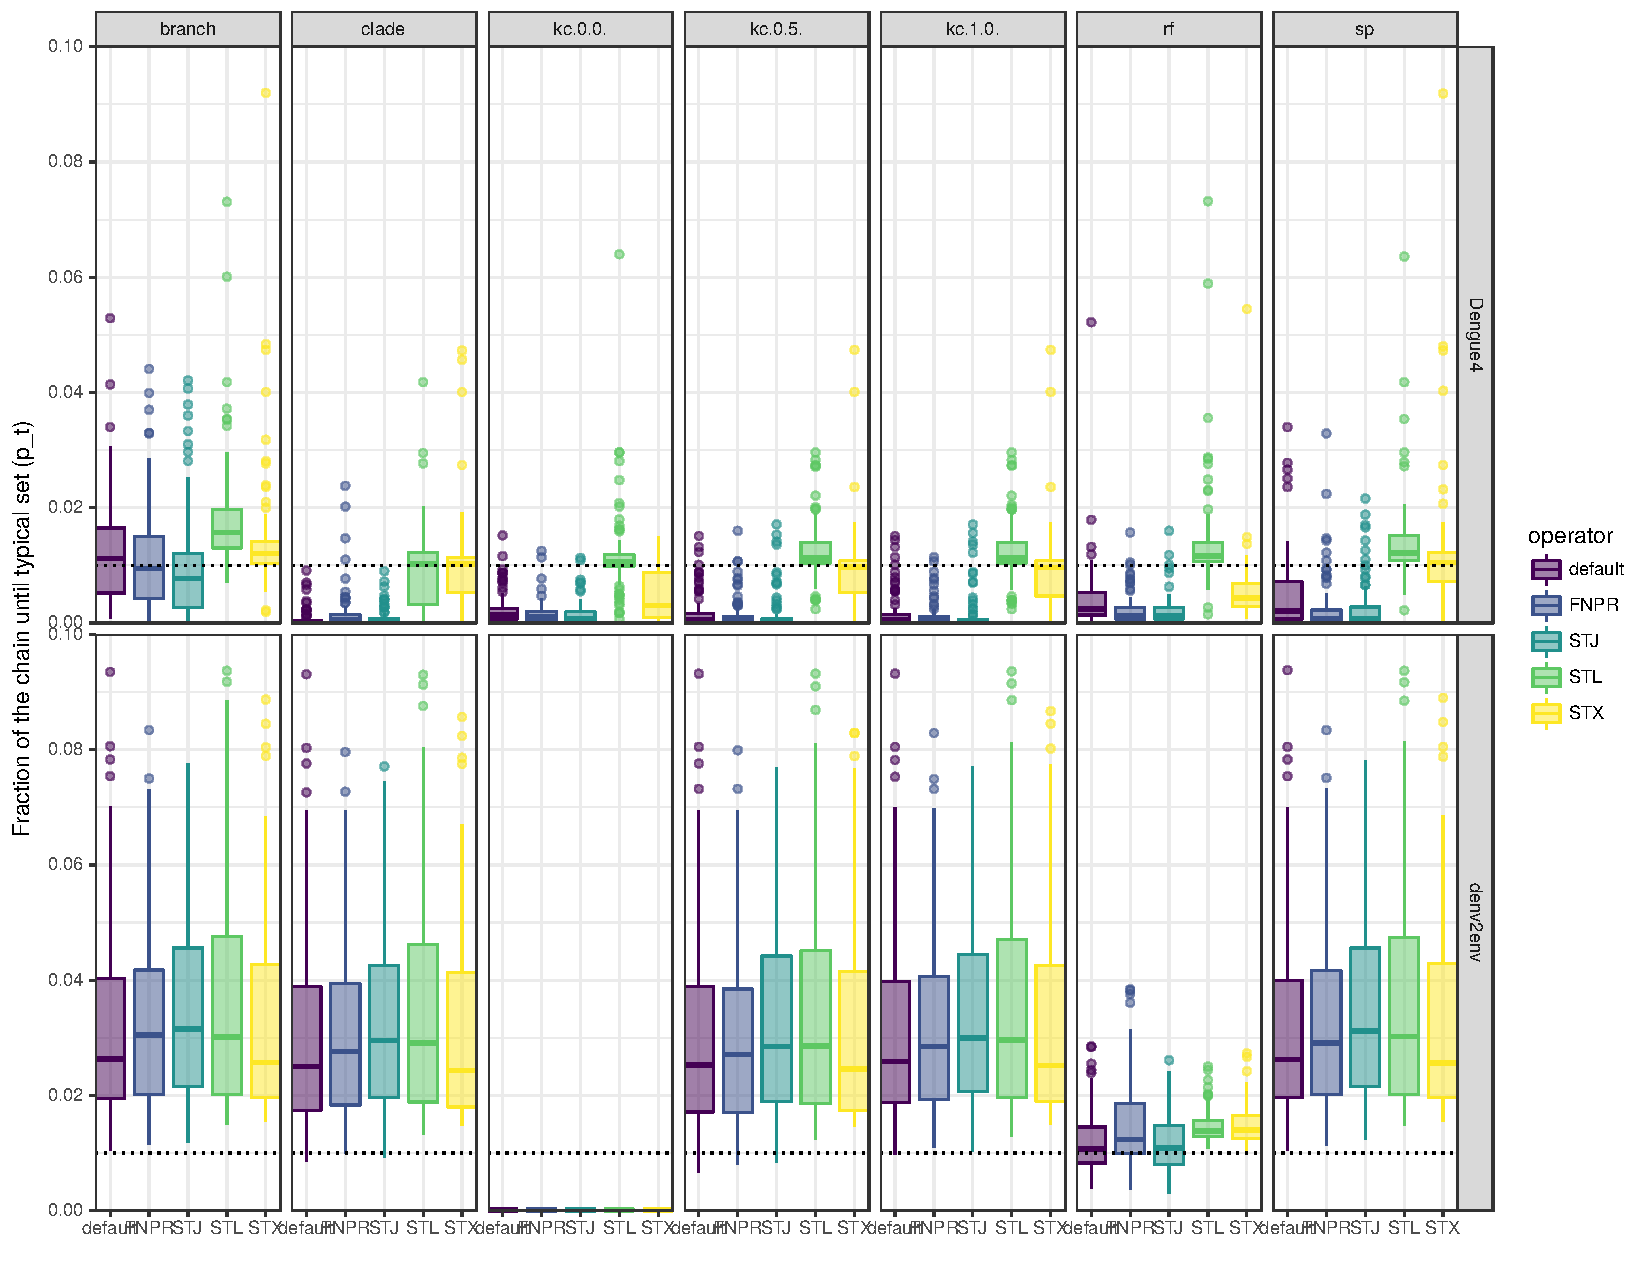
\includegraphics[scale=0.6]{\dir/figs/metrics_opt_warmup.pdf} 
\end{center}
 \caption[Fraction $p_t$ of the chain needed to hit the typical set (95\% CI) for several MCMC schemes and tree metrics.]{\textbf{Fraction $p_t$ of the chain needed to hit the typical set for several MCMC schemes and tree metrics.}
  Boxplots show the results of $100$ replicates per data set.
  Vertical tiles show different metrics and horizontal ones show different data sets.
  The dotted line shows a fraction of $1\%$ 
  }
of the chain, for comparison.
  Lower values show faster convergence.
 \label{fig:fractions_metrics}
\end{figure}

Moving on to efficiency measures, Figures~\ref{fig:distance_true_denv2_mean} and~\ref{fig:distance_true_denv4_mean} show the average distance attained after 50\% of the chain has been discarded as warm-up.
The smaller the distance attained, the better the estimates of the mean under a metric $d$ ($\mathbb{E}_\pi^d$), and the higher efficiency.  
The results show that \verb|STL| and \verb|STX| achieve lower distances and thus higher efficiency of sampling, for both data sets considered.
For the larger data set, with 90 taxa, the difference in performance is even larger (Figure~\ref{fig:distance_true_denv2_mean}).
These patterns remain more or less constant across metrics (e.g. KC, RF or SP), suggesting \verb|STX| outperforms the other MCMC schemes for both topology and branch length estimation. 

\begin{figure}[!ht]
\begin{center}
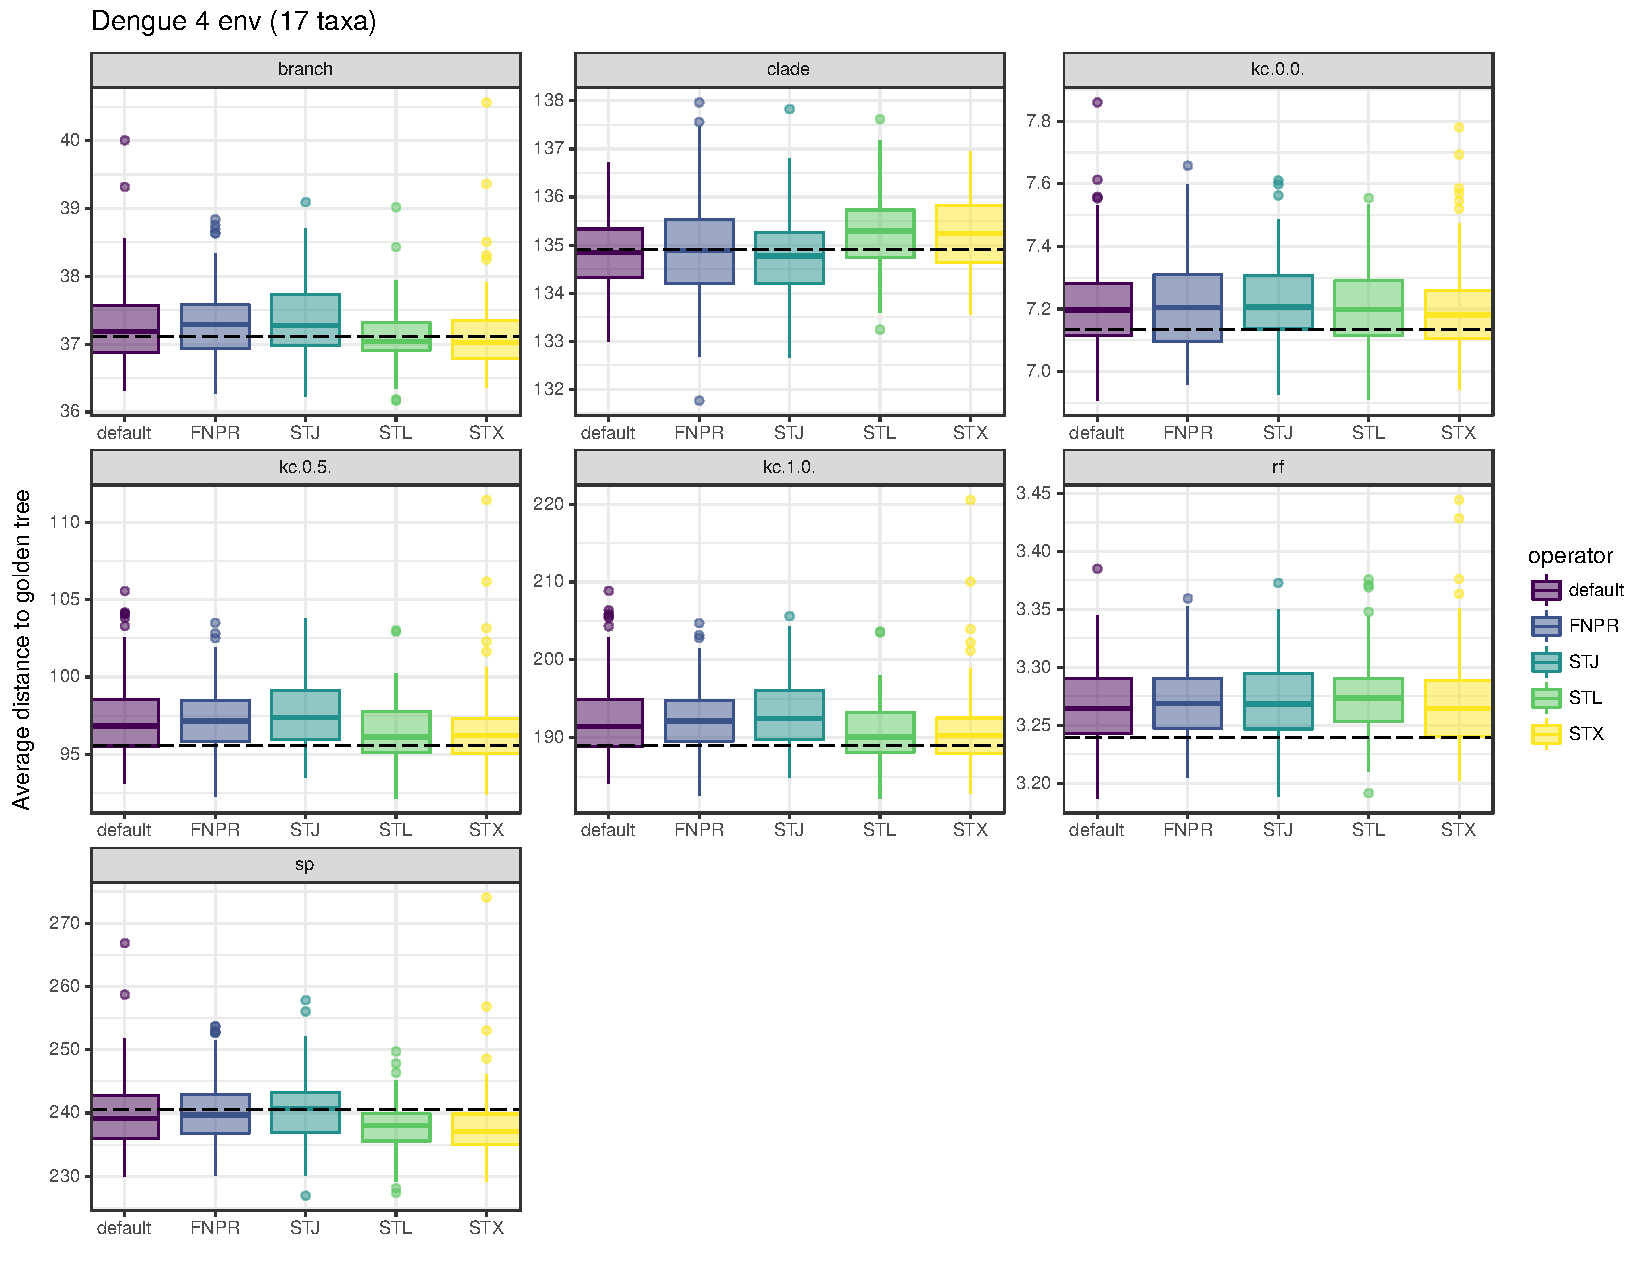
\includegraphics[scale=0.6]{\dir/figs/distance_true_denv4env_mean.pdf} 
\end{center}
 \caption[Average distance to true golden true tree for several MCMC schemes, Dengue 4 \textit{env} data set (17 taxa).]{\textbf{Average distance to true golden true tree for several MCMC schemes, Dengue 4 \textit{env} data set (17 taxa).}
  }
  Boxplots show the results of $100$ replicates per data set.
  Vertical tiles show different metrics and the dashed lines show the average distances to the true tree computed from the golden runs, i.e. the expectations of the target distributions shown in Figure~\ref{fig:target_golden}.
 \label{fig:distance_true_denv4_mean}
\end{figure}

\begin{figure}[!ht]
\begin{center}
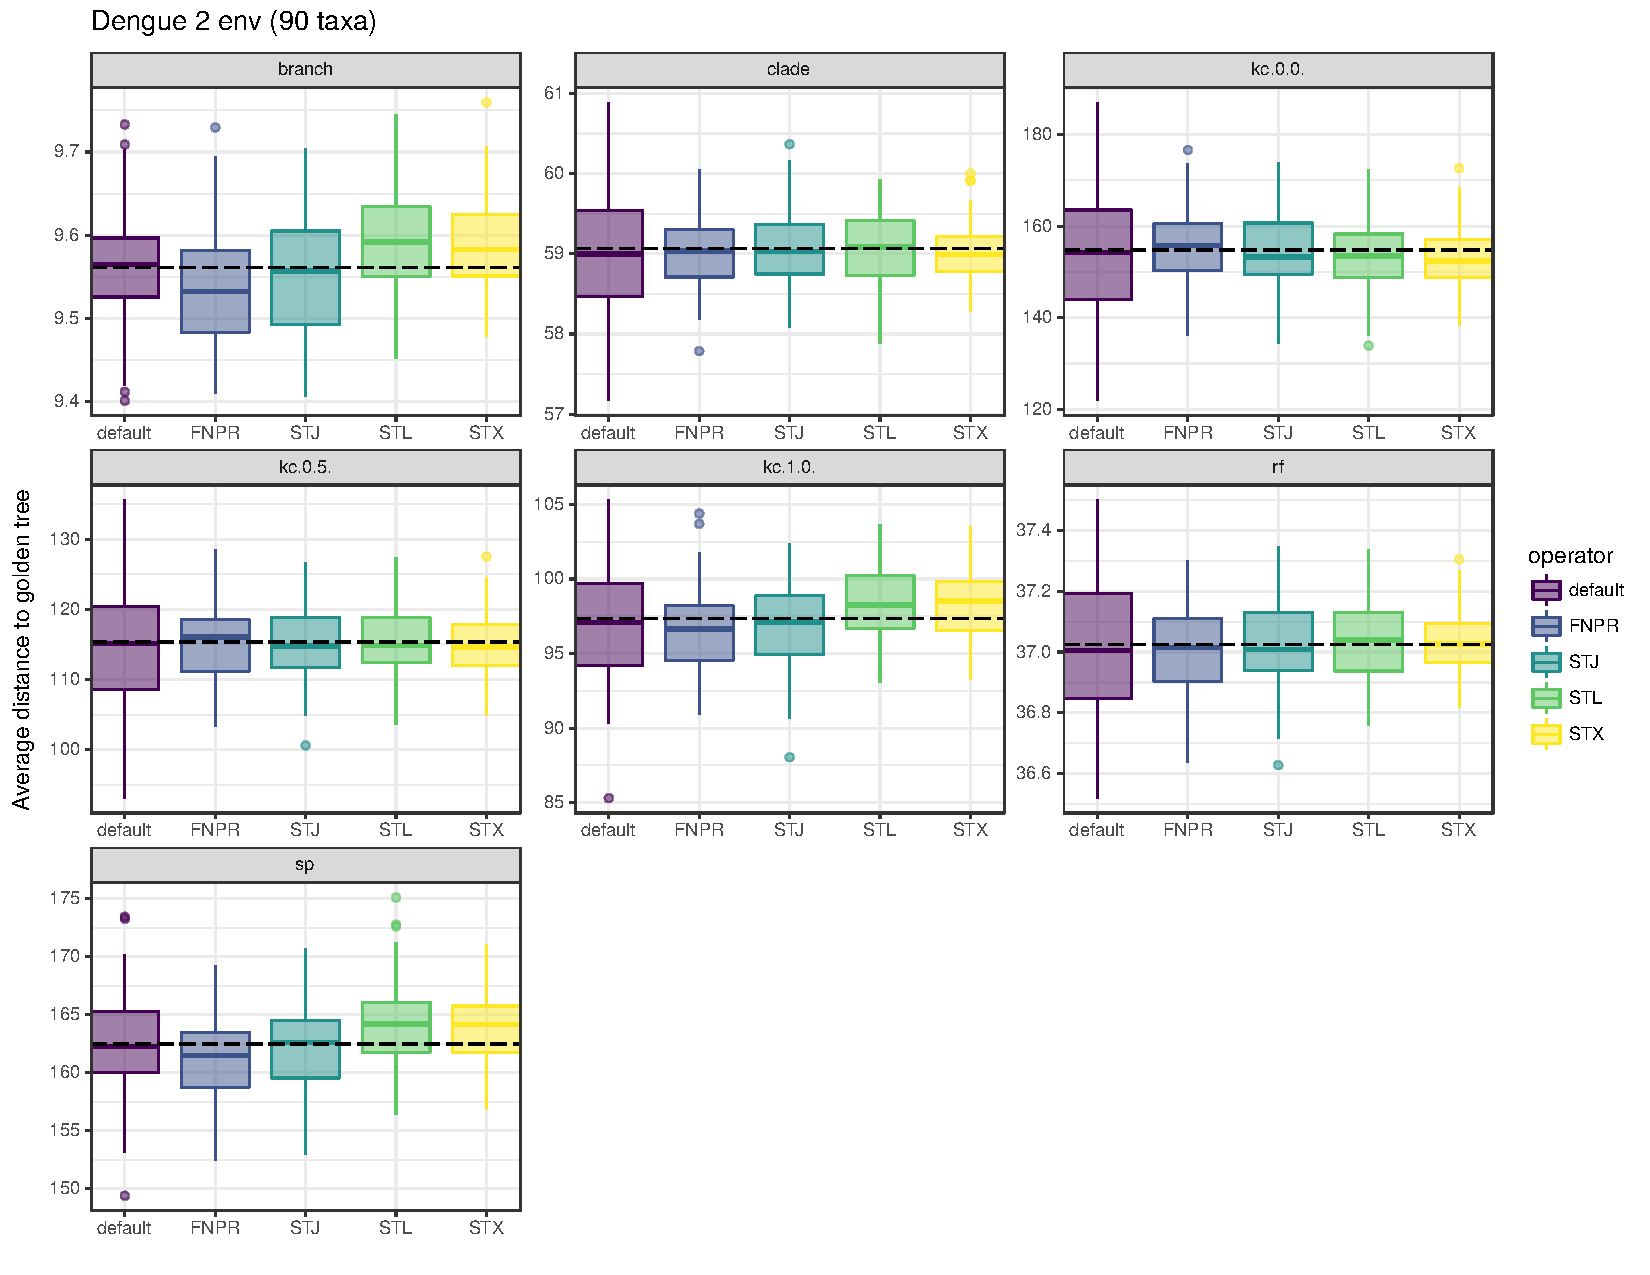
\includegraphics[scale=0.6]{\dir/figs/distance_true_denv2env_mean.pdf} 
\end{center}
 \caption[Average distance to true golden true tree for several MCMC schemes, Dengue 2 \textit{env} data set (90 taxa).]{\textbf{Average distance to true golden true tree for several MCMC schemes, Dengue 2 \textit{env} data set (90 taxa).}
  Boxplots show the results of $100$ replicates per data set.
  Vertical tiles show different metrics and the dashed lines show the average distances to the true tree computed from the golden runs, i.e. the expectations of the target distributions shown in Figure~\ref{fig:target_golden}.
  }
 \label{fig:distance_true_denv2_mean}
\end{figure}

The next step was to look at the effective sample size of the distance to the true (golden) tree, as measure of sampling efficiency in that space -- under various metrics.
This approach is similar to that of~\cite{Lanfear2016}, who call the ESS of the distance to a focal tree the ``pseudo ESS''.
The main difference is that here I take an MCC tree obtained from three very long (golden) runs as focal tree, instead of the first tree of the chain.
From Figure~\ref{fig:ESS_distance_true} we can see that while \verb|STL| displays better performance than the default scheme, the combination of \verb|STJ| and \verb|STL| (\verb|STX|) has the best performance in terms of the effective sample size of the distance to the true tree\footnote{Recall these are  MCC trees obtained from three separate golden runs.}.
This result seems to be consistent also for simulated data (see Figure~\ref{sfig:ess_true_50taxa} in Appendix B).
It seems also that as tree size grows the scaling of \verb|STX| becomes more important, as evidenced by some of the ESS from the default set of operators being below the common threshold of $200$ for some metrics (e.g. the KC metric with $\lambda = 0$).
If the one-dimensional projections of phylogenetic space provided by the target distributions shown in~\ref{fig:target_golden} are taken to be faithful representations of the original space then the results above indicate that \verb|STL| and \verb|STX|  allow more efficient sampling, not only in terms of distance to the true tree but also in number of effective samples per MCMC iteration.

\begin{figure}[!ht]
\begin{center}
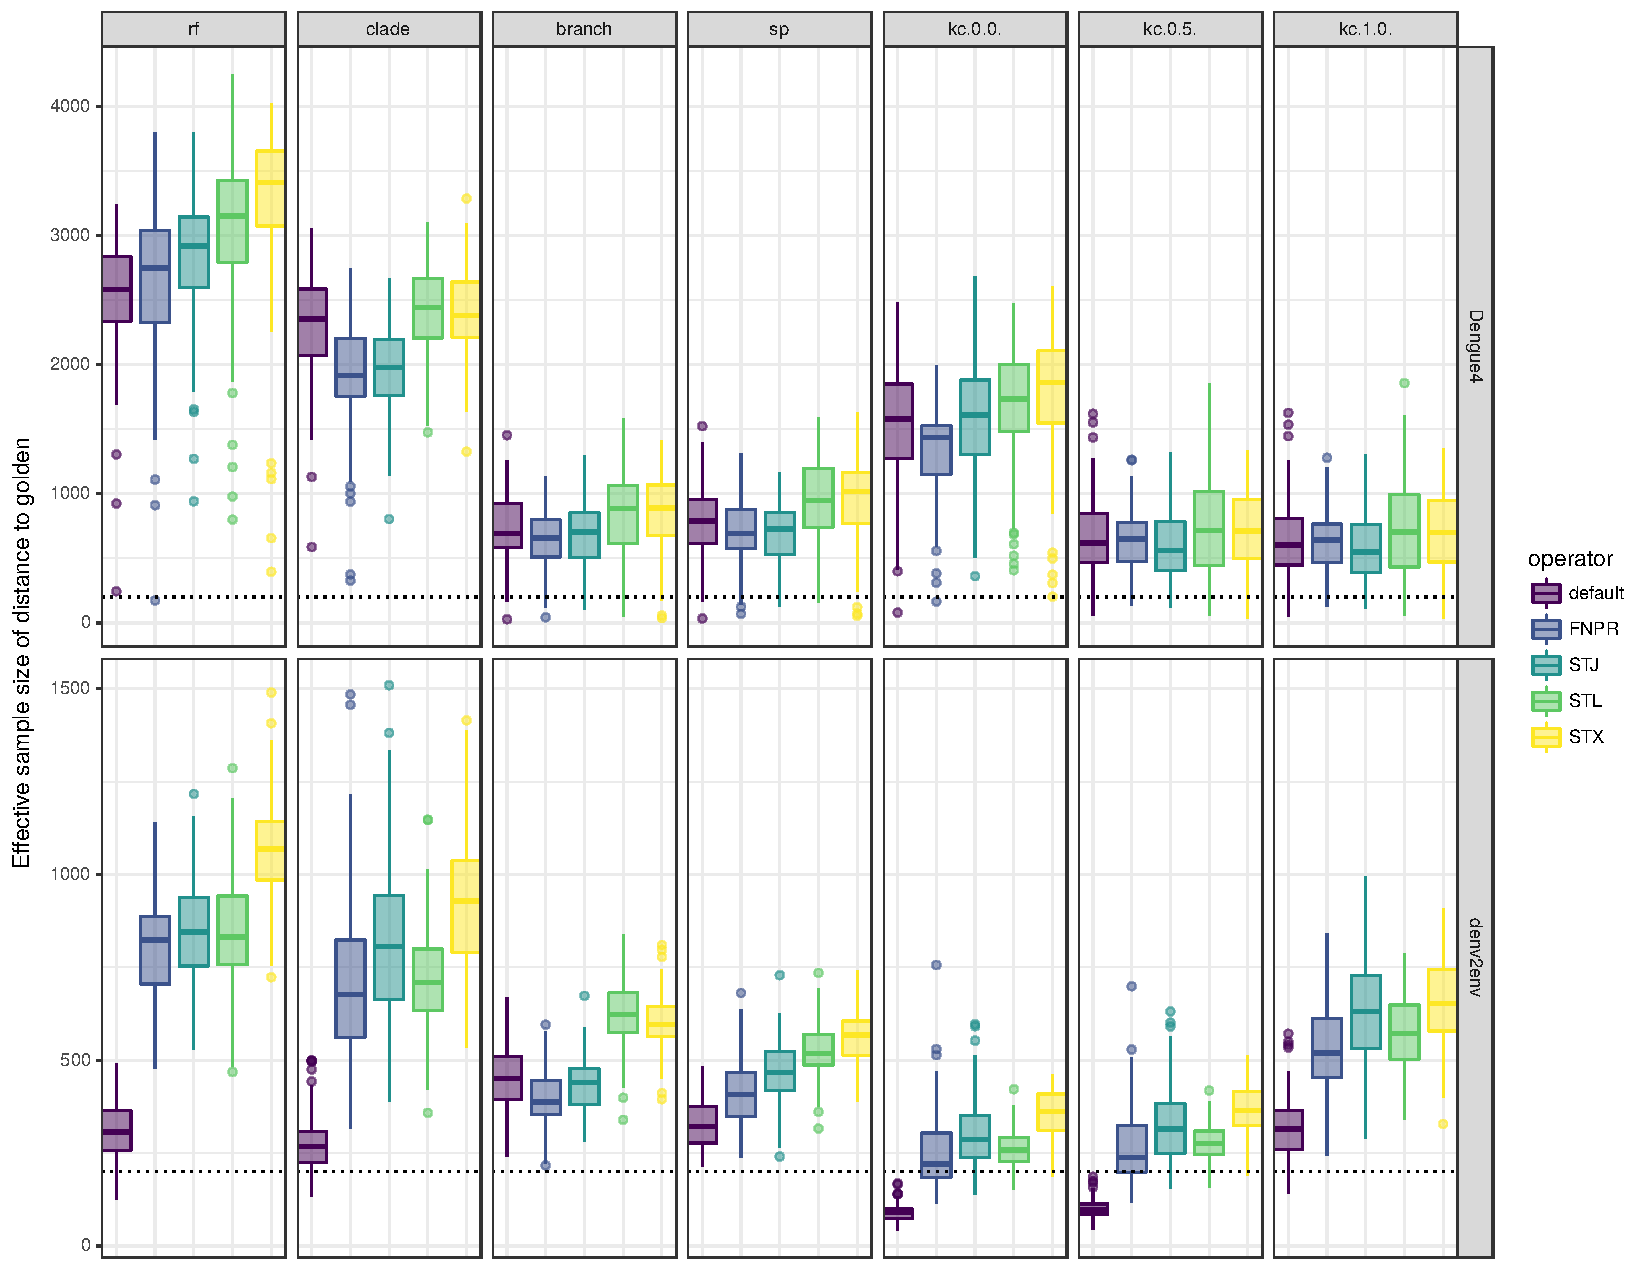
\includegraphics[scale=0.6]{\dir/figs/ESS_distance_true.pdf} 
\end{center}
 \caption[Effective sample size (ESS) of the distance to true golden true tree for several MCMC schemes.]{\textbf{Effective sample size (ESS) of the distance to true golden true tree for several MCMC schemes.}
   Boxplots show the results of $100$ replicates per data set.
  Vertical tiles show different metrics and horizontal ones show the two data sets studied in this experiment: DENV 4~\textit{env} (17 taxa) and DENV 2~\textit{env} (90 taxa).
  The dotted line marks the line $\text{ESS} = 200$.
  }
 \label{fig:ESS_distance_true}
\end{figure}

To further study performance in phylogenetic space, I analysed mixing in clade space.
The results in Figure~\ref{fig:mixing_clades} show several measures of performance, with panels A and B showing the rate of switching of clade absence/presence indicators (see Chapter 3, section~\ref{sec:cladeSwitch}) while panels C and D show the effective sample size of these clade indicators.
In theory, these measures should agree, since they are essentially measuring how quickly the chain explores clade space by visiting each clade proportional to its posterior probability; the faster the switching rate, the higher the ESS (see section~\ref{sec:cladeSwitch} in Chapter 3 for a discussion).
And we see that these quantities do agree and show that \verb|STL| and \verb|STX|  outperform the other schemes, specially for the larger data set.
On the other hand, the plots in Figure~\ref{fig:mixing_clades}E show that the two new schemes visit slightly fewer clades, but the difference seems to be smaller for the larger data set (see extended discussion).

\begin{figure}[!ht]
\begin{center}
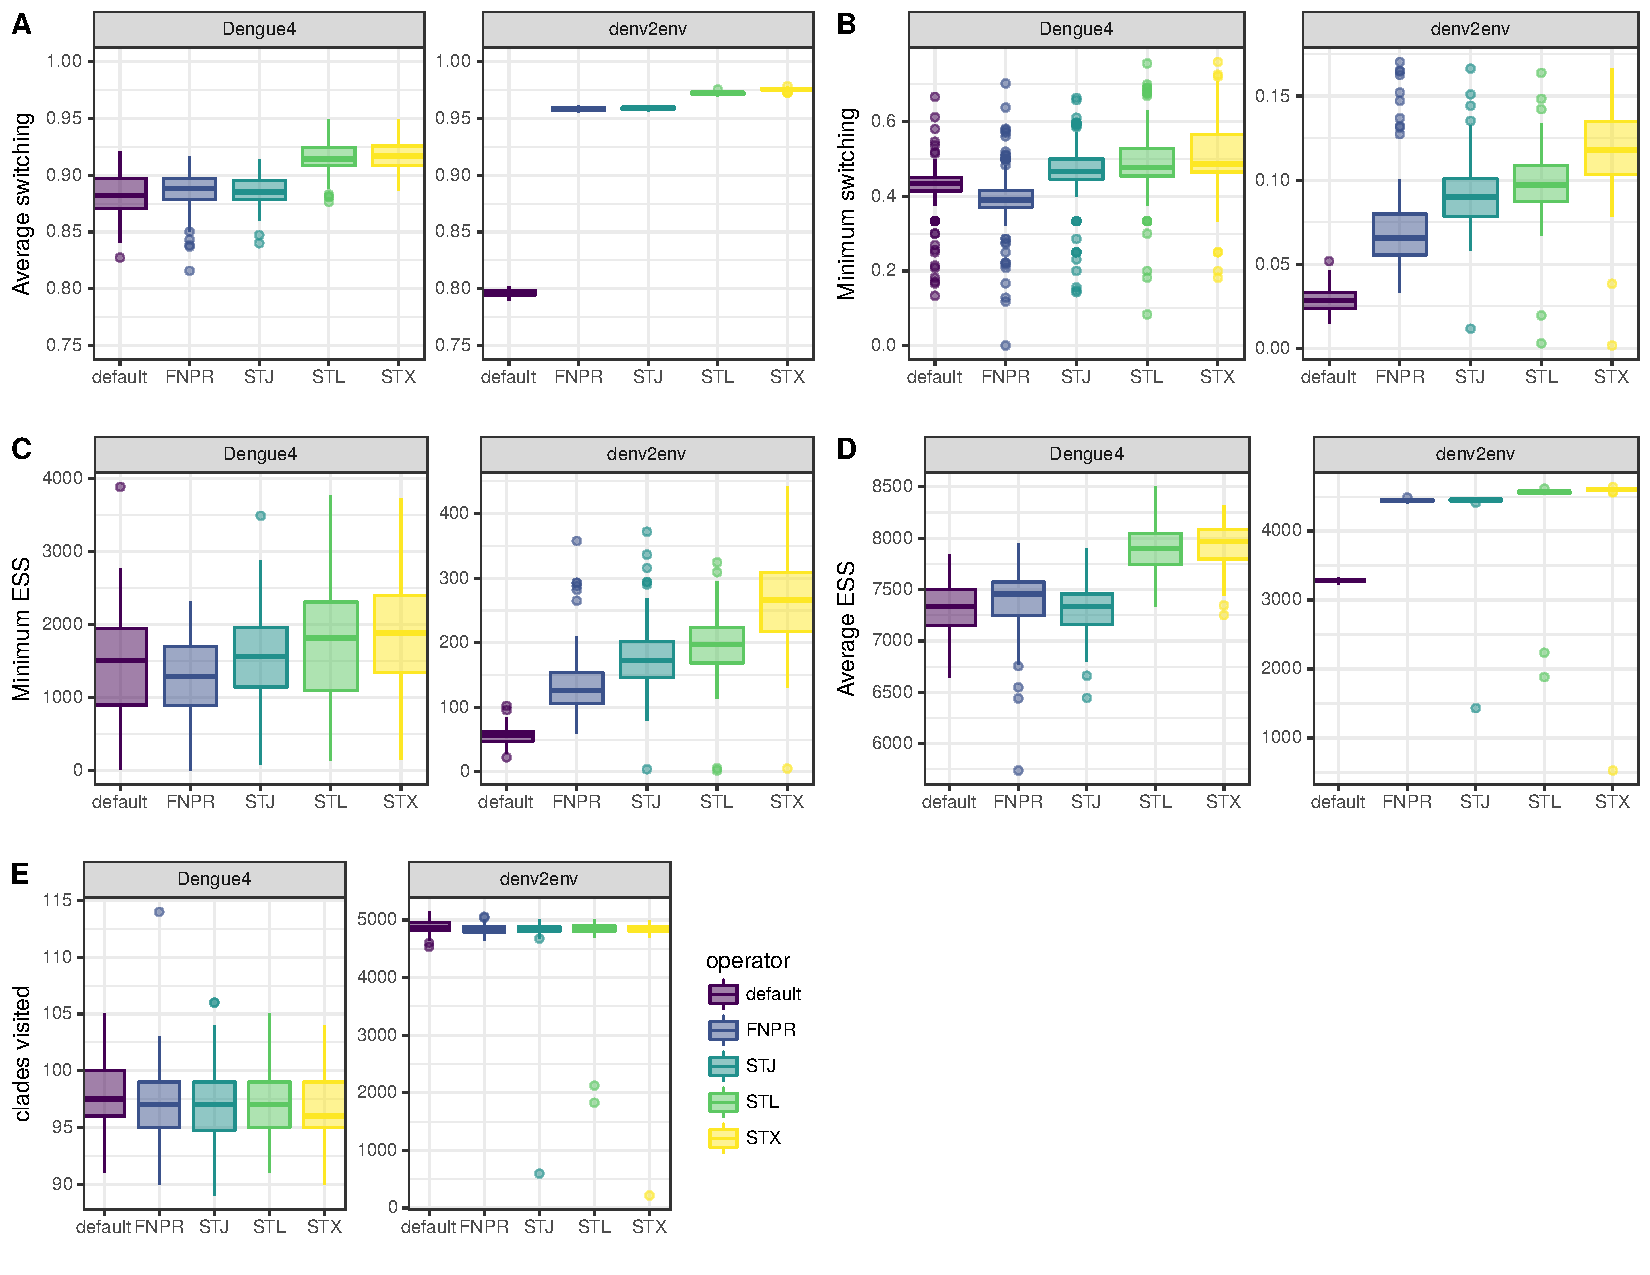
\includegraphics[scale=0.55]{\dir/figs/mixing_clades.pdf} 
\end{center}
 \caption[Measures of mixing in clade space for several MCMC schemes.]{\textbf{Measures of mixing in clade space for several MCMC schemes.}
  Boxplots show the results of $100$ replicates per data set.
  Horizontal ones show the two data sets studied in this experiment: DENV 4~\textit{env} (17 taxa) and DENV 2~\textit{env} (90 taxa).
  Panel A shows the average clade switching score (see Chapter 3 for definitions), while panel B shows the minimum -- across clades -- switching score.
  Panels C and D show the minimum and average ESS for the clade indicators, respectively.
  Panel E shows the total number of clades visited in a run of 10 (DENV-4, 17 taxa) or 20 (DENV-2, 90 taxa) million iterations with a sample of $10, 000$  phylogenies.
  Please note that y-axes differ between plots.
  }
 \label{fig:mixing_clades}
\end{figure}

While performance in phylogenetic space is the focus in this chapter, the ability to quickly traverse the space is also important regarding performance for other parameters that depend on the underlying phylogeny, such as growth and evolutionary rates.
I show that~\verb|STL| and~\verb|STX| can also facilitate the sampling of important continuous parameters that are dependent on the phylogeny, such as the mean evolutionary rate (\verb|meanRate|).
Figure~\ref{fig:continuous_ESS} shows the effective sample size for two continuous parameters: the mean evolutionary rate and the Gamma heterogeneity parameter $\alpha$  (\verb|CP3.alpha|) for the third codon partition.
While the evolutionary rate depends on all branch lengths and rate assignments over the tree and thus constitutes a hard parameter to sample, \verb|CP3.alpha| has very little dependence on the phylogeny (and other parameters in the model) and thus the chain usually converges quite quickly for this parameter.
The results show that while all MCMC schemes (operator mixes) perform comparably for \verb|CP3.alpha|,~\verb|STL| and~\verb|STJ| have improved performance for \verb|meanRate|.

I first looked at the fraction of the chain that, when removed as warm-up (burn-in), maximises the ESS, for a selection of continuous parameters (see Section~\ref{sec:performance_methods}), taking the maximum fraction across parameters as the measure for a particular run -- again, a conservative performance assessment.
The results are shown in Figure~\ref{fig:optimal_burnin} and reveal a slight advantage for \verb|STL| and \verb|STX| for the larger data set (DENV-2, 90 taxa).
Overall, however, this performance measure does not indicate substantial superiority of the new proposed schemes over the default.

\begin{figure}[!ht]
\begin{center}
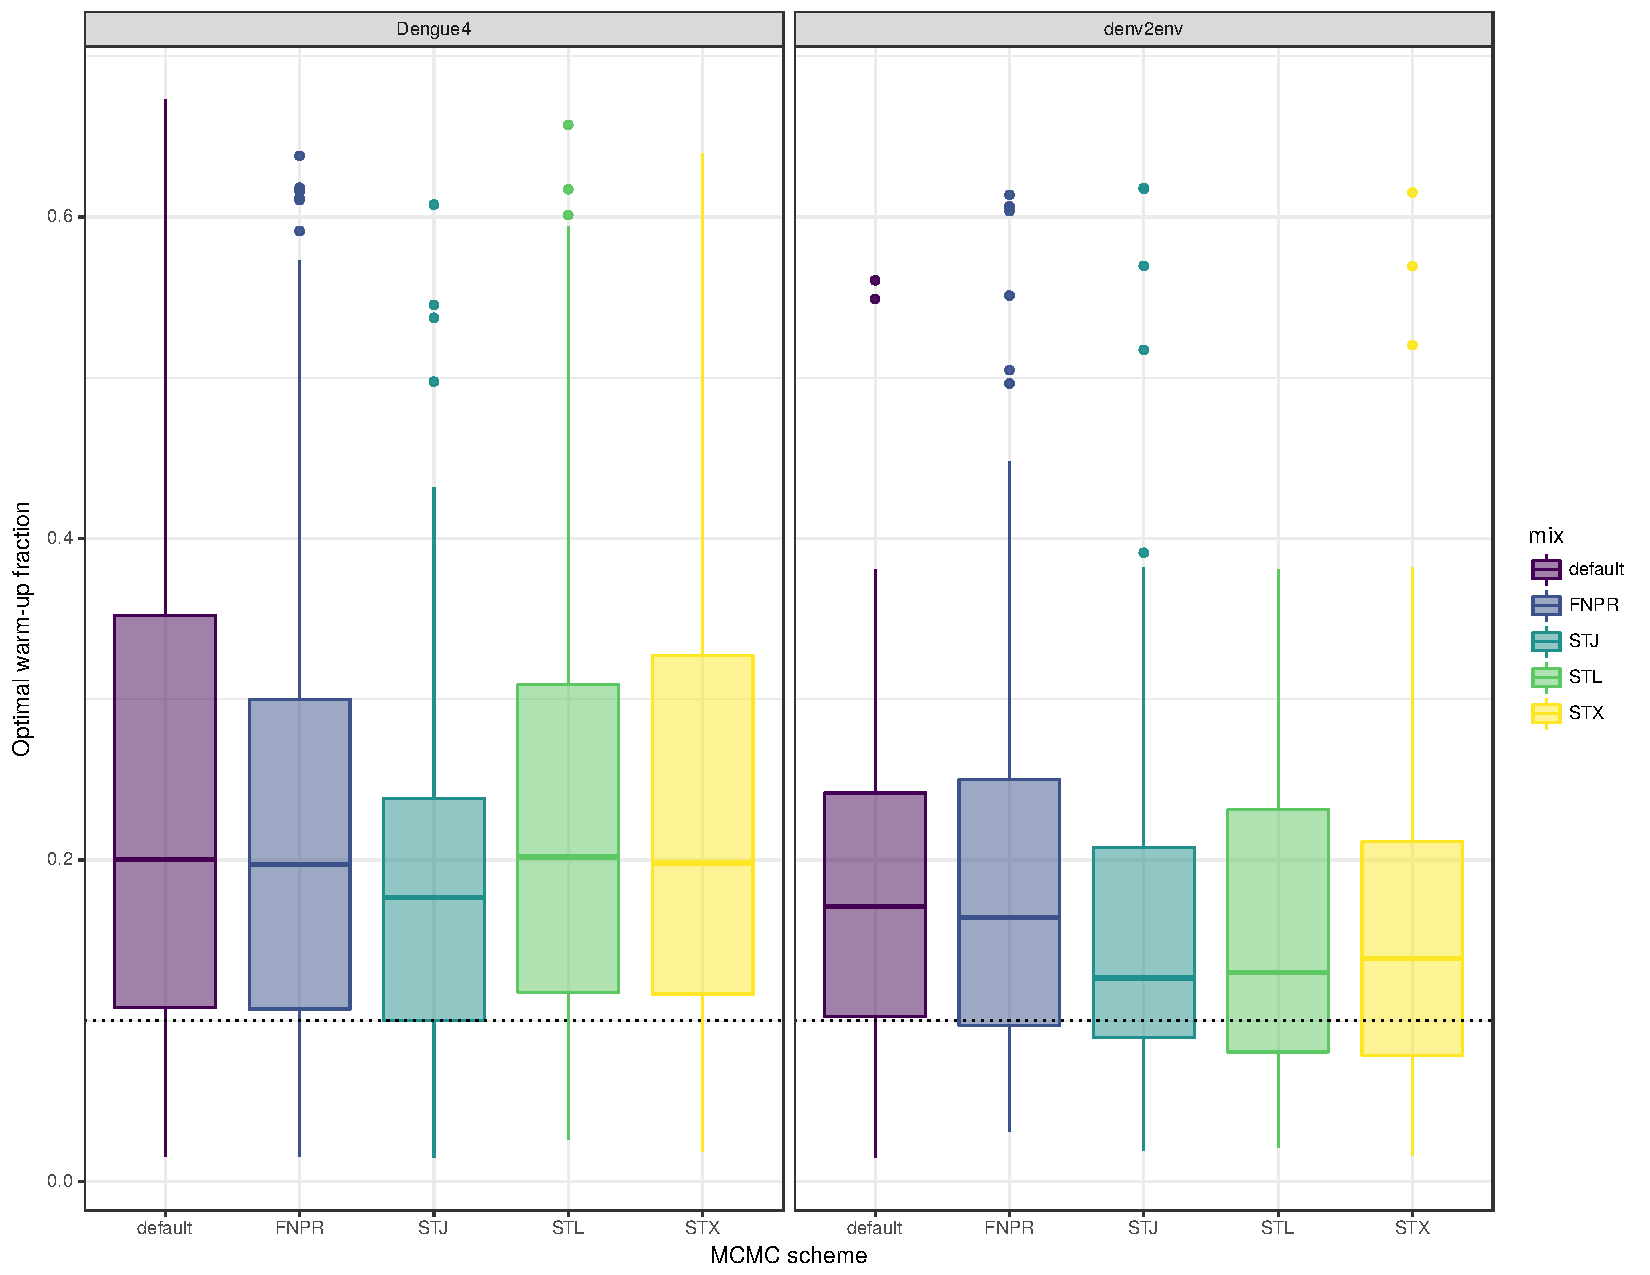
\includegraphics[scale=0.45]{\dir/figs/optimal_warmup.pdf} 
\end{center}
 \caption[Optimal warm-up (burn-in) fraction for several MCMC schemes, continuous parameters.]{\textbf{Optimal warm-up (burn-in) fraction for several MCMC schemes, continuous parameters.}
   Boxplots show the results of $100$ replicates per data set.
  Vertical tiles show the two data sets studied in this experiment: DENV-4~\textit{env} (17 taxa) and DENV-2~\textit{env} (90 taxa).
  See text for a description of how the optimal fraction was computed; lower values indicate better performance.
  The dotted line marks $10\%$, which is commonly discarded as warm-up (burn-in).
  }
 \label{fig:optimal_burnin}
\end{figure}

I then chose two continuous parameters to show the differences in efficiency between MCMC schemes by means of ESS for these parameters.
As an example of a parameter for which convergence is usually quick, I chose the Gamma heterogeneity parameter ($\alpha$) of one of the partitions\footnote{Both data sets (DENV-4 and DENV-2) were analysed under three codon partitions.} (\verb|CP3.alpha|) and I chose the mean evolutionary rate, averaged over all the branches of the phylogeny (\verb|meanRate|) as an example of a ``hard'' parameter, for which convergence and mixing are usually slow. 
The results, presented in~\ref{fig:continuous_ESS}, show that while for the ``easy'' parameter (\verb|CP3.alpha|, panel (a)) performance is consistent across MCMC schemes, for the ``hard'' parameter, which depends more strongly on the phylogeny, the new proposed schemes lead to higher ESS.
This is specially true for the larger data set (DENV-2, 90 taxa).
\begin{figure}[!ht]
\begin{center}
\subfigure[\textbf{Mean evolutionary rate}]{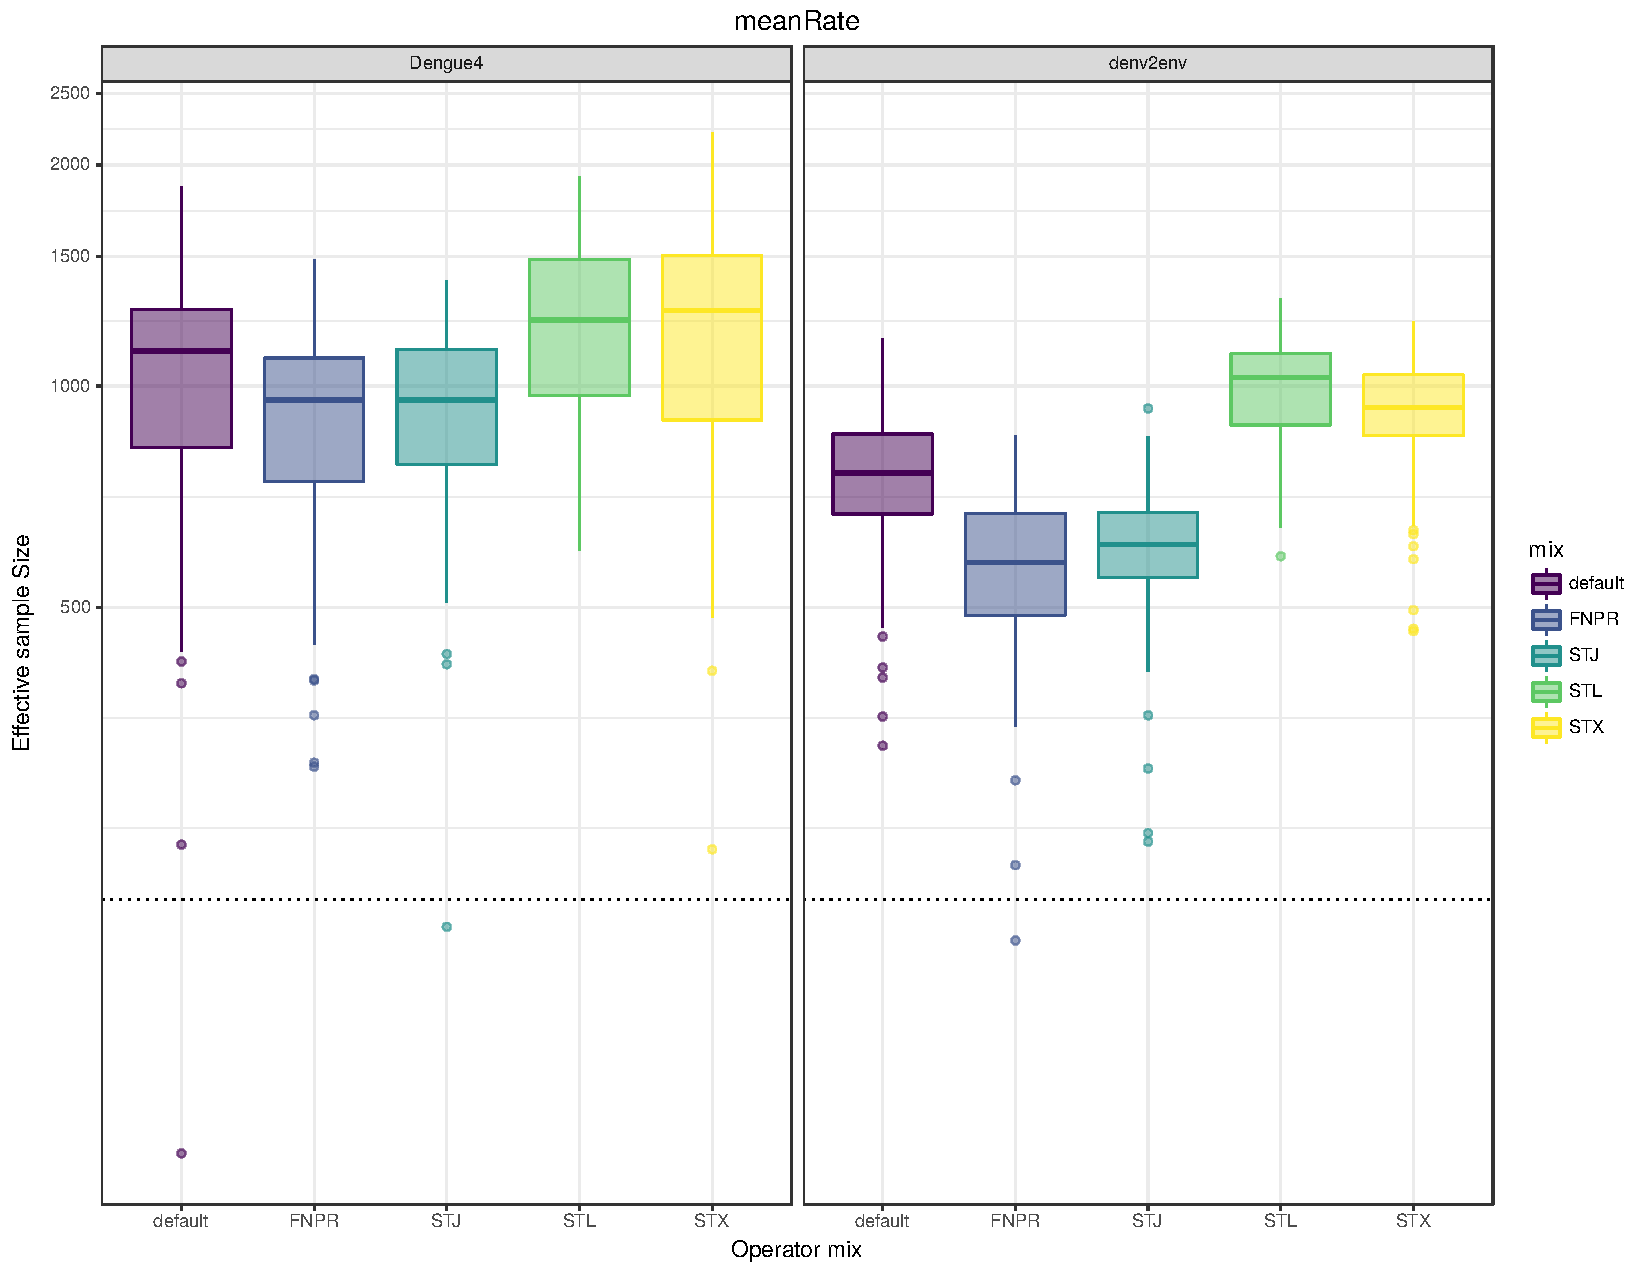
\includegraphics[scale=0.35]{\dir/figs/meanRate_ESS_performance.pdf}}
\subfigure[\textbf{Third coding partition $\alpha$ }]{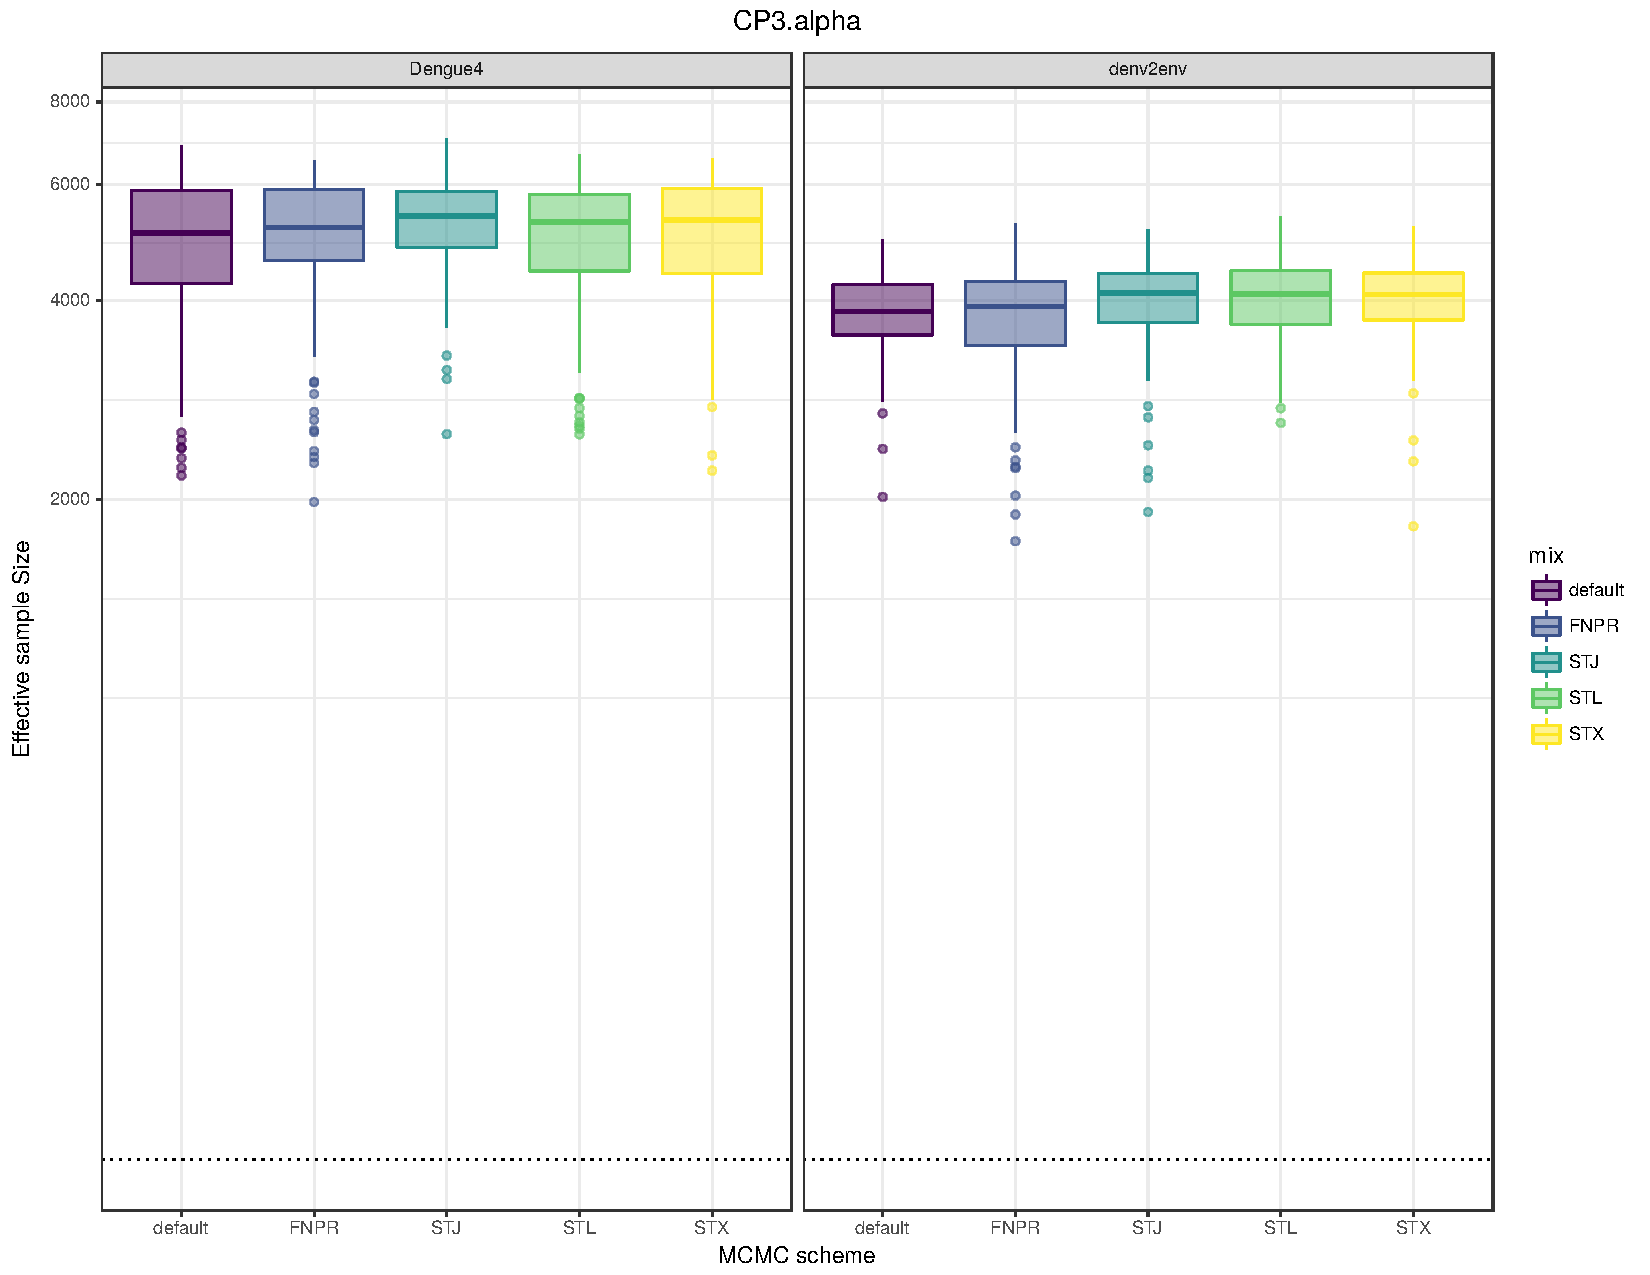
\includegraphics[scale=0.35]{\dir/figs/CP3Alpha_ESS_performance.pdf}}  
\end{center}
 \caption[Effective sample size (ESS) of continuous parameters for several MCMC schemes.]{\textbf{Effective sample size (ESS) of continuous parameters for several MCMC schemes..}
  Boxplots show the results of $100$ replicates per data set.
  Horizontal ones show the two data sets studied in this experiment: DENV-4~\textit{env} (17 taxa) and DENV-2~\textit{env} (90 taxa).
  The dotted line marks the line $\text{ESS} = 200$.
  Panel (a) shows the results for the mean evolutionary rate (meanRate) and panel (b) contains the results for the Gamma heterogeneity parameter $\alpha$ (CP3.alpha).
  }
 \label{fig:continuous_ESS}
\end{figure}

Some extra figures showing other results not discussed here can be found in Appendix B.

\section{Extended discussion}

Having already discussed some of the findings as I described them, in this section I shall expand on some aspects, focusing on a more general discussion.

\subsection{Adaptation issues}
\label{sec:STJadap}

While providing performance gains -- in terms of mixing -- individually, the new proposed schemes also showed considerable difficulty traversing phylogenetic space between modes.
This is most apparent in the results in Figure~\ref{fig:ebovmultimod}, where \verb|STL| (middle panel) gets stuck at lower mode, permanently on one chain and for a large portion of the run on another.
The results in Figure~\ref{fig:fractions_metrics} also show that the new schemes have longer warm-up periods.

Another problem we found during development and testing of \verb|STJ| is that for most data sets it was not possible to tune its scale parameter $\alpha$ (see Section~\ref{sec:newKernels}) to attain the desired acceptance probability of $0.234$.
This is in a way to be expected, because as mentioned above, the set of heights in a any given tree is ultimately discrete, hence not every acceptance probability is attainable.
As a workaround, for the EBOV (1610 taxa) analyses I set $\alpha = 0$, i.e., making \verb|STJ| essentially equivalent to \verb|FNPR|, barring differences in computational efficiency due to implementation.
This uniform \verb|STJ| when combined with \verb|STL| led to much better performance when compared to the default set of operators.

The results in Figure~\ref{fig:ebovmultimod} serve as a cautionary tale about the interaction between adaptive kernels and adaptation schemes for multimodal spaces: early adaptation can lead to poor exploration of the space, essentially blinding the algorithm to higher density modes.
The increased warm-up times could also be due to poor interaction with the adaptation schedule.
Investigating ways of cleverly setting initial values for the tuning (scaling) parameters could go a long way toward improving warm-up.
The findings in Section~\ref{sec:multimod} suggest that, in terms of the tuning parameter, the difference between a run that never finds a higher mode (run 3) and one that eventually does (run 2) is very small.
On the other hand, a bigger size such as the one attained by run 1 offers some protection against getting stuck at a lower mode, as expected.

The findings of Figures~\ref{fig:mixing_clades}E and~\ref{fig:fractions_metrics} when taken together, seem to suggest that the inability of \verb|STX| to explore more clades -- and hence, potentially, more topologies -- in the beginning of the chain could be the reason for larger warm-up times.
The adaptive nature of \verb|STL| means that it might sometimes get stuck on a mode because its size has been tuned for optimal sampling of that mode and larger jumps which are necessary for it to traverse the space between modes.
I hypothesise that the ability of the default operator mix and \verb|STX| to traverse phylogenetic space is conferred by non-tunable, bold transition kernels such as \verb|WideExchange| in the case of the default mix and \verb|SubtreeJump| in the case of \verb|STX|.
These may lead to big tree rearrangements and hence serve as crude mode-jumping kernels.
Crude in the sense that they are agnostic about the number and nature of the modes and hence lead to mode-jumping only occasionally and at random.
While \verb|STJ| -- and presumably also \verb|FNPR| --  helps jump modes, ideally we would like one single adaptive transition kernel that could be used alone with comparable or better performance.
It is in principle possible to design more guided candidate-generating mechanisms, which exploit the structure of the target distribution to avoid random-walk behaviour (see~\cite{Hoehna2012} and Chapter 6).

\subsection{Overall perspectives and future research}
\label{sec:performance_discussion}

Overall, the new schemes proposed in this chapter showed better performance, not only in phylogenetic space but also for continuous parameters of interest.
In particular, combining \verb|STJ| and \verb|STL| (\textit{i.e.} \verb|STX|) seems to prevent the pathological behaviour of getting stuck at lower modes while improving performance in a consistent manner.
These findings therefore point towards \verb|STX| as a more efficient MCMC scheme, in particular for larger data sets.
In most analyses, performance gains were bigger for the larger data set (DENV-2, 90 taxa).
Additionally, \verb|STX| considerably outperformed the default scheme for a challenging data set in the form of the EBOV data set which is comprised of 1610 full genomes.
Based on the available evidence, I hypothesise that gap in performance between the default scheme (operator mix) and \verb|STL| and \verb|STX| should increase as the size of the parameter space grows -- superexponentially -- with the number of taxa $n$.
This is because as the parameter space grows, the ability to avoid bold proposals and the resulting rejections becomes more and more important.
More technically, I predict that adaptive kernels are progressively more important to combat concentration of measure and the inherent bad scaling of MH methods.
More definitive conclusions, however, would depend on specific experiments to investigate scaling of different MCMC schemes as phylogenetic space grows in a controlled manner.
In addition, it would be very desirable to investigate the performance of several MCMC schemes for other large, challenging real-world data sets currently being compiled in phylodynamic studies, such as the large ($>15, 000$ genomes) HIV data sets collected by the PANGEA project~\citep{Pillay2015}.

A very important question, connected to what was discussed above, is the \textit{optimal scaling} of transition kernels for phylogenies, which might not be optimal for an acceptance probability of 0.234~\citep{Potter2015}.
While the ``0.234 result'' holds for a broad class of target distributions and MCMC schemes, it is not at all clear to me that the target distributions encountered in phylogenetics attain the necessary regularity conditions for the famous results of~\cite{Gelman1996} and \cite{Roberts1998} to hold.
Investigating this issue however would entail substantial development on the theoretical side, since comparatively to what is known for continuous multivariate distributions, we know very little about the geometrical properties of phylogenetic space~\citep{Gavryushkin2016, StJohn2017,Whidden2017}.
I shall touch on a few more issues regarding the application of MH-type algorithms to phylogenetics in Chapter 6.

Another elusive aspect of Bayesian phylogenetics is the correlation structure of the posterior when considering not only the interaction between topology and branch lengths but also dependence of parameters of interest such as $R_0$~\citep{Stadler2011} and the evolutionary rate on the phylogeny.
Results in Figures~\ref{fig:fractions_metrics} and~\ref{fig:optimal_burnin} do not agree: while \verb|STX| has longer warm-up times in phylogenetic space, it seems to lead to faster convergence for continuous parameters.
I do not know how to explain these results.
It could be that these experiments are not measuring exactly the same phenomenon, since the point from which the chain achieves its the maximum ESS can in theory be quite different from the point where it starts sampling from the typical set.
An experiment that characterised the target distribution for continuous parameters using golden runs in the same fashion as what was done in Figure~\ref{fig:fractions_metrics} could help clarify just how tied together convergence in phylogenetic space and convergence in continuous space are.
As a side note, despite giving a precise definition of the typical set in Chapter 1, I have opted to carry out the computations for the warm-up experiments using the (MCMC) time to reach the ``bulk'' of the distribution in the form of the 95\% credibility interval.
This is because computing the typical set for continuous distributions would entail extra computations and sensitivity analyses.
An interesting topic for future analysis would be to compute the typical set for the targets based on RF metric, which are discrete and for which the entropy is easier to compute, and compare these with the 95\% CI.

Finally, in order to see ways for improving our methods, it is of vital importance that we revisit the arbitrary choices made along the way so as to see ways in which generalisation is possible.
The first aspect that could be investigated is the balancing between \verb|STJ| and \verb|STL| in terms of weighting: there is no particular reason why the weighting I have used here (Table~\ref{tab:operator_mixes}) is optimal.
It could in fact be the case that one needs to change the relative weighting of the operators as the number of taxa grows, for instance.
Another arbitrary choice was made in the distance kernel distribution used in \verb|STL|.
The choice of a half-Gaussian could easily be relaxed, and any continuous distribution with positive unbounded support could be used.
\cite{Yang2013} for instance propose the use of the so-called ``bactrian'' distributions, which are bimodal distributions for which the ``peakness'' of the density (\textit{i.e.} the separation between the modes) can be controlled by a tuning parameter $m$, which could be adapted in much the same way as $\sigma$ for \verb|STL| or $\alpha$ for \verb|STJ|.
These distributions could in theory help the chain get out of lower modes by allowing big jumps occasionally
A further arbitrary choice made in the construction of \verb|STL| is to choose the destination node uniformly.
There is also no particular reason why the probability of re-grafting $P_i$ at $P_j \in \mathbf{D_i}(\delta)$ should not depend on the actual distance between $P_i$ and $P_j$.
While investigation of the impact these choices on overall performance is of great interest, it would also entail a large amount of experiments to adequately address.

In summary, this chapter provides the following contributions:
\begin{itemize}
 \item Compiled challenging real-world data sets that better reflect those encountered in practice; 
 \item Proposed an improved framework for checking the correctness of a phylogenetic transition kernel;
 \item Proposed a framework for evaluating MCMC performance for phylogenetics that circumvents limitations of previous approaches (see also Chapter 3);
 \item Provided a new adaptive candidate-generating mechanism that updates topology and branch lengths simultaneously.
 \item Showed improved performance of the proposed candidate-generating mechanisms for challenging real-world data sets.
\end{itemize}

See Chapter 6 for a more general discussion of the relevance of the findings here in the field of Bayesian phylogenetics.

% \bibliography{/home/max/Dropbox/PHD/THESIS/bibliography/lmcarvalho_PhD_Thesis}

\renewcommand{\dir}{../chapter3/chapter/}
\chapter{Convergence diagnostics for Markov Chain Monte Carlo in Bayesian phylogenetics: the case of time-trees}

\epigraph{It is unbelievable that this stubborn darkness, this eternal eclipse, this flaw in geometry, this eternal cloud on virgin truth can be endured.}{Farkas (Wolfgang) Bolyai (1775-1856) talks about proving the parallel postulate in a letter to his son J\'anos Bolyai (1802-1860).}


%%%%%%%%%%%%%%%%%%%%%%%%%%%%%%%%%%%%%%%%%%%%%%%%%%%%%
%%%%%%%%%%%%%%%%%%%%%%%%%%%%%%%%%%%%%%%%%%%%%%%%%%%%%
\section{Motivation}
\label{sec:intro}

Markov chain Monte Carlo (MCMC) methods have become a standard tool for approximating complex posterior distributions encountered in Bayesian inference~\citep{Robert2011}.
In phylogenetics, most if not all Bayesian approaches rely on MCMC for approximating the posterior distribution of trees~\citep{Li2000,Suchard2001,Huelsenbeck2001b}.
These methods rely on constructing a Markov chain whose stationary distribution is the (target) distribution one wishes to sample from.
A fundamental issue is to determine when the chain has reached stationarity and samples are being drawn from the target distribution.
Whilst much attention has been given to this issue in the statistical literature, most diagnostic methods assume univariate, continuous parameter spaces.
Discrete, high-dimensional parameter spaces such as those encountered in phylogenetics pose additional challenges to development of effective convergence diagnostic tools.
In her review of the geometry of tree space, \cite{StJohn2017} argues that the power of the tree/phylogeny model ``comes from the property that adds the complexity: the vast number of trees to explain different possible evolutionary scenarios'' (pg e83).
As argued by~\cite{Drummond2015}, the complexity of phylogenetic space can be seen as a major reason for the development of specialised software for Bayesian phylogenetics as opposed to the use of common Markov Chain Monte Carlo (MCMC) packages such as Stan~\citep{Carpenter2017} and JAGS~\citep{Plummer2003}. 

Available methods for diagnosing convergence of MCMC for Bayesian phylogenetics include tracking clade (split) frequencies both within and between chains~\citep{Nylander2008}, multi-dimensional scaling of tree distance matrices~\cite{Hillis2005,Matsen2006} and network-based clustering~\citep{Whidden2015}. 
These methods are mostly graphical in nature, and only recently have more formal convergence metrics been proposed~\citep{Whidden2015,Lanfear2016}.
An important thing to notice is that it is not possible to say with complete certainty when a Markov chain has converged to its target distribution.
Rather, convergence tools are designed to identify failure to converge.
As argued by~\cite{Mossel2005}, when the data do not conform with the model (e.g., come from a mixture of trees rather than a single tree) apparent convergence can be misleading.
\cite{Cowles1996} and~\cite{Brooks1998} further reinforce the point that multiple convergence diagnostics need to be employed in order to mitigate the risk of determining convergence when in fact chains have not reached the desired target.
Thus, no single method or tool is likely to supersede all the others, as there are cases where one method fails to detect problems but others identify failure to converge. 
Successful application of convergence detection tools fundamentally depends on combining several metrics/tools in one coherent framework~(e.g. the approaches of~\cite{Nylander2008} and~\cite{Lanfear2016}).
An additional issue with currently available methods is that most assume either unrooted trees and/or contemporaneous sequences, limiting their applicability in cases where one deals with time-calibrated phylogenies (time-trees).
While~\cite{Warren2017} attempt to integrate most of the popular visualisation methods -- along with some quantitative indicators -- into one framework, their approach is infeasible for large time-calibrated phylogenies.

This chapter is a companion to Chapter 2, where I discuss transition kernels for Metropolis-Hastings MCMC and employ several of the methods described/developed here to assess convergence and performance.
My goal here is to expand upon their approach and make the necessary adaptations to accommodate time-calibrated trees with hundreds of taxa.
In what follows I review  some key concepts in Bayesian phylogenetics as well as the state-of-the-art for convergence diagnostics in MCMC applied to Bayesian phylogenetics.
I then proceed to discuss the limitations of available methods when dealing with time-calibrated trees and suggest adaptations.
My ultimate goal is to investigate a statistically useful representation of tree space and develop an analysis pipeline that can aid practitioners diagnose their MCMC runs when performing phylodynamic analyses for the increasingly larger data sets found in practice.

\subsection{Tree metrics}
\label{sec:metrics}

A key step in characterising phylogenetic space is constructing valid metrics on it.
A tree (phylogeny) metric is a mapping $d_\sigma : \boldsymbol \Psi \times \boldsymbol \Psi \to [0, \infty)$ that satisfies (i) $d_\sigma(u, v) \geq 0$; (ii) $d_\sigma(u, v) = 0 \iff u = v$;  (iii) $d_\sigma(u, v) = d_\sigma(v, u)$ and (iv) $d_\sigma(u, w) \leq d_\sigma(u, v) + d_\sigma(v, w)$ for any pair of trees $u, v$. 
For convenience, I let $\sigma$ be an indexing parameter so that we can distinguish between different metrics and study their properties.

A comprehensive review of available tree metrics would be infeasible.
Instead, I review a few important metrics that capture different aspects of phylogenetic space.
\cite{Robinson1981} propose a metric to compare unrooted tree topologies based on a tree operation $\alpha(u, v)$ that removes (contracts) all edges from $u$ that are not present in $v$, creating $u \wedge v$.
The reverse operation $\alpha^{-1}$ in turn adds edges to $u \wedge v$ to create $v$.
Let $n_\alpha$ and $n_{\alpha^{-1}}$ be the numbers of $\alpha$ and $\alpha^{-1}$ operations between $u$ and $v$.
Then the Robinson-Foulds (RF) metric is $d^{\text{RF}}(u, v) = n_\alpha + n_{\alpha^{-1}}$.
In other words the RF metric counts (twice) the number of internal branches/edges that differ between two phylogenies.
Another important tree metric is the so-called subtree prune-and-regraft (SPR)~\citep{Allen2001}.
Similarly to the above, let $\beta$ be an operation that picks an edge $e$ in $u$, prunes the subtree subtended by $e$ and regrafts this subtree at another edge $f$, creating a new tree $v$.
The SPR metric between $u$ and $v$ counts how many $\beta$ operations are necessary to turn $u$ into $v$. 
SPR is biologically interpretable and can also be used to construct useful representations of phylogenetic space (see Section~\ref{sec:graph}).
While there exist relatively efficient fixed parameter algorithms, computing the SPR metric is NP-hard.
As with the RF metric, SPR only captures differences in branching order (topology), not branch lengths.

To address this limitation,~\cite{Kuhner1994} proposed to calculate the square root of the sum of the squared differences of the internal branch lengths corresponding to shared bipartitions between $u$ and $v$.
While this adaptation does allow comparing branch lengths, it includes topological differences only implicitly.
As an advantage however is that there are very efficient, linear time algorithms available to compute the KF distance between pairs and lists of trees~\citep{Pattengale2007}.
In their excellent review of analytical results on tree metrics,~\cite{Steel1993} propose a simple and easy to compute metric that accounts for branch length differences, called the~\textit{path length} difference metric, henceforth called Steel-Penny (SP).
Let $d_{ij}^\tau$ be the sum of branch lengths separating tips $i$ and $j$ in phylogeny $\tau$. 
The SP metric computes the squared differences of path lengths by two trees $x$ and $y$ as $d_{\text{SP}}(x, y) = \sqrt{\sum_{1 \leq i \leq j \leq n} (d_{ij}^x - d_{ij}^y)^2 }$.

\cite{Kendall2016} proposed a new metric that can be thought of as a compromise in terms of applicability and computational complexity and that allows for the comparison of topology and branch lengths at the same time by cleverly encoding the phylogenies.
For a phylogeny $u$, define $m_{i,j}$ to be the first node which is simultaneously the parent of $i$ and $j$,~\textit{i.e.}  $m_{i,j}$ is the most recent common ancestor (MRCA) of $i$ and $j$.
Then we are prepared to construct the vector with all $n(n-1)/2$ unique pairs of MRCAs, supplemented by $n$ entries with value $1$ at the end,  $\boldsymbol m(u) = \{ m_{1,2}, m_{1, 3}, \ldots, 1, 1, \{ $n$\:\text{times} \}, 1 \}$.
Let $W_{i,j}$ be the branch length associated with $m_{i,j}$ and define $l_i$ to be the root-to-tip path length for tip $i$ in $u$.
Then we can define\footnote{Hence $|\boldsymbol m(u)| = |\boldsymbol W(u)| = n(n+1)/2$.} $\boldsymbol W(u) = \{W_{1,2}, W_{1,3}, \ldots, l_1, \ldots, l_n \}$.
For $ 0 \leq \lambda  \leq 1$ we can combine topology and branch length and encode the phylogeny $u$~\textit{via} the vector $\boldsymbol\eta_\lambda(u) = (1-\lambda)\boldsymbol m(u) + \lambda \boldsymbol W(u)$.
Finally, we are prepared to define the Kendall-Colijn (KC) metric between two phylogenies $u$ and $v$ as $d_\lambda^{\text{KC}}(u, v) = ||\boldsymbol\eta_\lambda(u) -\boldsymbol\eta_\lambda(v)||$, where $||\cdot||$ is the the Euclidean or $L^2$ norm.
This metric combines topology and branch lengths, is continuous for any $\lambda \in [0, 1]$ and is straightforward to compute, specially when compared with the BHV and SPR metrics.

Finally, I describe two other metrics specifically designed for time-calibrated trees.
The first, which I shall call the clade-difference (CD) metric, asks for two phylogenies $\tau_A$ and $\tau_B$, how many different clades there exist and how different their heights are.
More formally, let $\boldsymbol C(x)$ be the set of clades of phylogeny $x$.
Then the CD metric can be defined as follows: for each clade $c_i \in \boldsymbol C(\tau_A)$, compute the height of the MRCA between the constituents of $c_i$ in $\boldsymbol C(\tau_B)$, $m_i$ and the corresponding clade in $\tau_A$.
Repeating the same procedure for $\tau_B$ we can then compute:
$$ d_{\text{CD}} (\tau_A, \tau_B) = \sqrt{  \sum_i\left[ \left(h(c_i) - h(m_i) \right)^2 \right]  + \sum_j \left[ \left(h(c_j) - h(m_j)\right)^2 \right].  } $$
The idea behind CD is to quantify big topological differences such that  if a clade moves  across the tree, the metric will penalise both the difference between the height of that node and the root in $\tau_A$ and back down to the height of the corresponding node in $\tau_B$.
The second metric is the rooted branch score (BS) was proposed by~\cite{Heled2010} and computes the Euclidean distance in branch lengths between shared clades.
Let $b(\tau, c)$ be the length of the branch subtending $c$ in $\tau$ if $c \in \boldsymbol C(\tau)$ and $0$ otherwise.
Then we are prepared to define
$$d_{\text{BS}}(\tau_A, \tau_B) = \sqrt{ \sum_{c \in \boldsymbol C(\tau_A) \cup \boldsymbol C(\tau_B) } \left( b(\tau_A, c) - b(\tau_B, c) \right)^2 }  .$$
Fortunately, efficient implementations do exist for these metrics, e.g. in the JEBL library (\url{https://github.com/rambaut/jebl2}).

\section{Convergence of Markov chain Monte Carlo methods} % Related work
\label{sec:litrev}

I now move on to review the existing literature on quantifying and visualising MCMC convergence for Bayesian phylogenetics.
My main goal is to explore how several approaches capture different aspects of the process under analysis and discuss their shortcomings when dealing with the types of phylogenies I am interested in this thesis: time-calibrated phylogenies, with large numbers of taxa and complex tip sampling structures.
Before I proceed, however, it is important to make clear that one can never positively assert the convergence of a finite Markov chain to a stationary distribution.
In contrast, convergence detection/assessment is done in a negative fashion: one~\textit{fails to detect lack of convergence} and hence asserts that~\textbf{the chain appears to have converged}.
Another important remark is that~\textbf{convergence is a global feature},~\textit{i.e.} for high-dimensional models with many parameters, one can only assert that the run appears to have converged if that is true of \textit{all} parameters.

\subsection{Convergence diagnostics for continuous parameters}
\label{sec:continuous}

In Bayesian phylogenetics, sometimes researchers are interested in gathering inference about what I will hereafter call ``continuous parameters''\footnote{Called ``scalar estimands'' elsewhere~\citep{Gelman2014b}. Here, however, I am also interested in vector-valued quantities, such as root probabilities, population sizes,  etc.}.
These include evolutionary and migration rates, Markov evolutionary model parameters (e.g. $\kappa$ in the HKY model), amongst many others.
Fortunately, this kind of parameter is the standard in models used in the statistical literature at large, which means there is a large body of work on how to detect convergence for continuously-defined quantities in MCMC (see~\cite{Cowles1996} and~\cite{Mengersen1999} for reviews).

Let $\boldsymbol\theta = \{\theta^{(1)}, \theta^{(2)}, \ldots, \theta^{(M)}\}$ be a collection of $M$ samples from a single run of MCMC.
Since from a Bayesian perspective all computations should be done from the target posterior $\pi$ (see Chapter 1), we need to make sure that $\boldsymbol\theta$ is a sample from that distribution.
The first thing to notice is that the samples in $\boldsymbol\theta$ are~\textit{correlated} and hence do not constitute a proper sample from the target.
Hence we need to quantify the amount of~\textit{autocorrelation} between the samples, which in turn will give us an estimate of the~\textit{effective} number of samples from $\pi$ contained in $\boldsymbol\theta$, \textit{i.e.} for any $n \leq M$ we want to assess the dependence between $\theta^{(n)}$ and $\theta^{(n + 1)}$.
I will now make these statements precise, following the notation of~\cite{Geyer2011} as much as possible, occasionally borrowing from the Stan manual~\citep{StanTeam2017} as well.

It is often the case with MCMC that we are interested in quantity $Y = g(\theta)$, where $g(\cdot)$ a real-valued function, but the distribution of $Y$ cannot be derived analytically and hence expectations of the form $\mu = E[g(X)]$ cannot be computed exactly. 
An estimate of $\mu$ can be obtained from $\boldsymbol\theta$ as:
\[ \hat{\mu}_M = M^{-1}\sum_{i = 1}^M g(\theta^{(i)}). \]
If the samples in $\boldsymbol\theta$ were independent, we could say that $\hat{\mu}_M \approx \text{Normal} (\mu, \sigma^2/M)$ using the central limit theorem (CLT).
However, because by construction the samples are correlated, we need to take that into account when estimating the variance of $\hat{\mu}_M$.
Let $\gamma_k = \text{cov}(g(\theta^{(i)}), g(\theta^{(i + k)}))$ be the autocovariances and write the variance $\sigma^2$ as 
\[ \sigma^2 =  \gamma_0 + 2\sum_{k=1}^\infty \gamma_k,\]
and the autocovariances can in turn be estimated as 
\begin{equation}
\label{eq:autocovs}
 \hat{\gamma}_k = M^{-1}\sum_{i = 1}^{M-k}[g(\theta^{(i)}) - \hat{\mu}_M][g(\theta^{(i + k )}) - \hat{\mu}_M]
\end{equation}

With a estimate $\hat{\sigma}_M$ of the variance we can then define the \textbf{effective sample size (ESS)}:
\begin{align}
 \label{eq:ESSa}
 n_{\text{eff}} &= M\frac{\sigma^2}{\hat{\sigma}_M}, \\
  \label{eq:ESSb}
 &= \frac{M}{ 1 + 2\gamma_0^{-1}\sum_{k = 1}^\infty \gamma_k},
\end{align}
which captures the number of samples in the MCMC sample $\boldsymbol\theta$ that are effectively independent and hence can be used for inference\footnote{In practice the upper limit of the summation in the denominator of Eq (\ref{eq:ESSb}) is substituted by a finite bound $K$. See~\cite{Geyer2011} and references therein for details on the determination of $K$ and the estimation of $n_{\text{eff}}$.}.
In Bayesian phylogenetics practice, ESS is at the core of most convergence assessment -- for continuous parameters --, the common recommendation being that all parameters in a MCMC run have $n_{\text{eff}} > 200$.
The rationale for this recommendation seems to be that the variability in most quantities of interest is such that a sample size of $200$ should allow for precise computation of most functionals.
In this chapter I will use the \verb|effectiveSize()| in the~\textbf{coda} package~\citep{Plummer2006} and the routines in the package Tracer v1.7~\citep{Rambaut2018} to compute ESSs.

While the ESS is a useful tool for assessing convergence, it is designed to deal with one chain (run) at a time.
A powerful technique for assessing convergence is to run several parallel chains from overdispersed starting points and determine whether they converge to the same distribution.
Suppose $K$ runs of $M$ iterations each are available, \textit{i.e.}, we have $\boldsymbol\theta_i, i = 1, 2, \ldots K$.
The between sample variance can be written as
\begin{equation}
\label{eq:Between}
 B = \frac{M}{K-1} \sum_{k = 1}^K \left(\bar{\theta}_k - \bar{\bar{\theta}}\right)^2, 
\end{equation}
where $\bar{\theta}_k = M^{-1}\sum_{i = 1}^M\theta_k^{(i)}$ and $\bar{\bar{\theta}} = K^{-1}\sum_{k=1}^K\bar{\theta}_k$.
Now we can define the within variance as 
\begin{align}
\label{eq:Within}
 W &=  K^{-1}\sum_{k = 1}^K s_k^2,\\
 s_k^2 & = (M-1)^{-1} \sum_{i = 1}^M \left(\theta_k^{(i)} - \bar{\theta}_k\right)^2.
\end{align}
Finally we can define the~\textbf{potential scale reduction factor} (PSRF)~\citep{Gelman1992}:
\begin{equation}
 \label{eq:PRSF}
 \hat{R} = \sqrt{\frac{ (M-1)W +  B }{MW}}.
\end{equation}
At convergence, $\hat{R} < 1.1$, providing a univariate measure of convergence across chains (for a given parameter).

Finally, I note  that we are usually interested in complex models, where correlation between parameters is frequently a feature of the posterior.
I detail the approach of~\cite{Vats2015} that attempts to provide an overall measure of convergence by means of a~\textbf{multivariate effective sample size (mESS)}.
The idea is to accommodate posterior dependence between parameters by jointly considering all parameters at once and estimating their variance-covariance matrix.
For $M$ samples, the mESS is defined as :
\begin{equation}
 \label{eq:multiESS}
 n_{\text{eff}}^m = M\left(\frac{\text{det}(\boldsymbol\Lambda)}{\text{det}(\boldsymbol\Sigma)}\right)^{1/p},
\end{equation}
where $p$ is the number of parameters under analysis and $\text{det}(\boldsymbol\Lambda)$ and $\text{det}(\boldsymbol\Sigma)$ are the determinants of the sample covariance matrix and the Monte Carlo covariance matrix, respectively.
Notice that similar to the ESS, when samples are independent, $\boldsymbol\Lambda = \boldsymbol\Sigma$ and hence $ n_{\text{eff}}^m = M$.
Routines to compute the mESS are implemented in the R package~\textbf{mcmcse}~\citep{Flegal2017}.

Notice that these procedures can be used to determine the lower bound on the multivariate ESS to achieve a certain level of confidence.
If $\epsilon$ is the fraction of the variance due to Monte Carlo error and we would like to collect enough samples to have $(1-\alpha)\times 100 \%$ confidence, the bound becomes
\begin{equation}
 \label{eq:mESSbound}
  n_{\text{eff}}^m  \geq \frac{\pi2^{2/p}}{(p \Gamma(p/2))^{2/p}} \frac{\chi^2_{1-\alpha, p}}{\epsilon^2},
\end{equation}
where $\Gamma(\cdot)$ is the (analytically continued) Gamma function and  $\chi^2_{1-\alpha, p}$ is the appropriate quantile of a chi-squared distribution with $p$ degrees of freedom.
For instance, if $p=1$ and one would like for the Monte Carlo error to be no more than $5\%$ ($\epsilon = 0.05$) of the total variance and would like to have $95\%$ confidence, we would need an ESS of at least $6146$.
If Monte Carlo error is allowed to be $10\%$ ($\epsilon = 0.10$) the minimum required ESS decreases to $1516$, a figure more than seven times higher than the folkloric recommendation for $\text{ESS} \geq 200$ in phylogenetics\footnote{See for instance~\url{http://beast.community/analysing_beast_output}.}.
If one adopts this recommendation --\textit{i.e.} fixes ESS = 200 --, keeping $\alpha = 0.05$ gives $\bar{\epsilon} = 0.27$, meaning this recommendation leads to inferences being drawn from samples where nearly 30\% of the variance is due to Monte Carlo error.

\subsection{Convergence in phylogenetic space}
\label{sec:treespaceconv}

I now move on to present the state of the art for convergence metrics specifically designed for phylogenetics.
Their limitations are also explicitly discussed.

\subsection{Clade frequencies}
\label{sec:awty}

When diagnosing MCMC convergence in phylogenetic space, simply inspecting the traces for, say, the phylogenetic likelihood, might be misleading because two phylogenies with similar likelihoods may not be necessarily close in phylogenetic space.
The approach of~\cite{Nylander2008} is to analyse clade/split frequencies to this end.
The program AWTY (short for ``are we there yet?'') developed by~\cite{Nylander2008} provides graphical facilities for assessing convergence by analysing various aspects of the distribution of sampled clades.
I shall describe and discuss these features now.

For $ i = 1, 2, \ldots, |\boldsymbol C|$, let $\boldsymbol X_i = \{X^{(1)}, X^{(2)}, \ldots, X^{(M)}\} \in [0, 1]^M$ be a collection of samples from a Markov chain such that $X^{(j)}_i = 1$ if clade $i$ was sampled in the $j$-th iteration and $0$ otherwise.
Also, for $s_i = \sum_k X_i^{(k)}$ we call $f_i = s_i/M$ the \textit{frequency} of clade $i$.
By plotting clade frequencies estimated in two independent runs against each other (scatterplot), one can assess whether both chains have converged to similar distributions.
Lack of convergence can be detected when points fall away from the identity ($x = y$) line.
For a single run, one useful diagnostic is plotting cumulative clade frequencies along the chain.
If these trajectories present long-term trends\footnote{I am not familiar with the original implementation of AWTY, but this could be made precise by for instance applying LOESS-based trend detection methods to the trajectories.}, it means clade frequencies have not stabilised, indicating lack of convergence.

When multiple (say $K$) runs are available, a very common univariate summary associated with clade frequencies is the \textbf{average standard deviation of split frequencies  (ASDSF)}:
\begin{equation}
 \label{eq:ASDSF}
%  C^{-1}\sum_{i = 1}^{C} \sqrt{(K-1)^{-1}\sum_{k=1}^K\left(f_{ik} - K^{-1}\sum_{k = 1}^K f_{ik}\right)^2}
 \delta_C = (K-1)^{-1/2}\sum_{i = 1}^{C}\sqrt{\sum_{k=1}^K\left(f_{ik} - K^{-1}\sum_{k = 1}^K f_{ik}\right)^2}
\end{equation}
where $C$ is the number of clades seen in all runs.
ASDSF is employed for instance in the software \verb|Mr Bayes|~\citep{Huelsenbeck2001a}, where an ASDSF of less than $0.01$ is taken as sign of convergence -- and used as a stopping rule.

Absence-presence plots show whether a particular clade was absent or present in the tree sampled at each iteration of the chain.
If there are long periods where the clade is either absent or present, this indicates the chain has not mixed well and might not have converged.
On the other hand, a trace plot of this kind where the indicator variable frequently switches between $0$ and $1$ indicates good mixing.
This notion of ``clade-switching'' can be made more precise (see section~\ref{sec:cladeSwitch}).
It should be noted however that tracking all clades present in a given run becomes exponentially more cumbersome as the number of taxa increases, quickly overwhelming any graphical diagnostic capabilities.

Finally, one can also plot the (phylogenetic) distance within and between runs using any of the metrics described above.
The idea is, again, that at convergence these sets of distances should be similar, and I discuss below (Section~\ref{sec:treeESS}) how to make this notion mathematically precise following~\cite{Whidden2015}.
In short, AWTY provides the following diagnostics: (i) scatterplot of clade frequencies; (ii) plot of cumulative  clade frequencies; (iii) absence-presence plots for clades and (iv) tree distances between and within runs.
See Figure 1 in~\cite{Nylander2008} for a graphical summary.
A modern incarnation of AWTY, RWTY~\citep{Warren2017} seeks to provide modern plotting routines to implement the AWTY framework in the R language.
RWTY also integrates other techniques not available from AWTY like multi-dimensional scaling visualisation (see below).
The implementation of RWTY is amenable to automation, insofar as it allows easy scripting and report generation using capabilities available for R.

\textbf{Limitations}

Most methods in AWTY (and RWTY) are visual, and hence do not provide precise quantitative measures to guide researchers toward a decision.
This in turn also means that these procedures are hard to automate, what hinders their application in automatic phylogenetic pipelines such as \verb|NextStrain|~\citep{Hadfield2017}.
As an example, consider the clade frequency scatter plots described above: what is an acceptable bound on the deviations in clade frequencies between two independent runs?
This question could be tackled with theoretical considerations and/or a careful empirical study, but neither~\cite{Nylander2008} nor~\cite{Warren2017} offer any insight into the matter.

\subsection{Clade switching}
\label{sec:cladeSwitch}

Here I describe  what to the best of my knowledge is a new metric for quantifying mixing in clade space.
Let $\boldsymbol X_i = \{X^{(1)}, X^{(2)}, \ldots, X^{(n)}\} \in [0, 1]^n$ be a collection of samples from a Markov chain such that $X^{(j)}_i = 1$ if clade $i$ was sampled in the $j$-th iteration and $0$ otherwise.
Also, for $s_i = \sum_k X_i^{(k)}$ we call $f_i = s_i/n$ the \textit{frequency} of clade $i$.
For $m_i = \min(n - s_i, s_i)$, it can be shown that the maximum number of transitions that can be observed from $\boldsymbol X_i$ is either $J_i = 2 m_i$
\footnote{Technically, $J_i$ depends on the first state $X_i^{(1)}$.
Suppose w.l.o.g. that $m_i = s_i$.
Then $J_i = 2 m_i - 1$ if $X_i^{(1)} = 1$ and $J_i = 2 m_i$ otherwise.
}.

When the chain is mixing well,~\textit{i.e.}, efficiently traversing phylogenetic space, we expect the indicators to be flipping between $0$ and $1$ as frequently as possible,  the maximum frequency depending on $f_i$.
Let $\delta_i = \Delta(\boldsymbol X_i)$, where $\Delta(\cdot)$ a function that counts the number of state transitions in $\boldsymbol X_i$.
Then $\sigma_i = \delta_i/J_i \in [0, 1]$ is a score that measures the relative efficiency of sampling by comparing how how many transitions happened compared to the theoretical maximum. 
This metric is quite similar to the Split Swap Rate of~\cite{Hoehna2008b}.

If the data are very informative, it is possible that some clade will have very high or very low posterior probabilities, meaning their indicators might never change.
These clades are not interesting for assessing mixing and I therefore restrict attention to clades with $0.4 \leq f_i \leq 0.8$.
This choice of ``interesting clades'' is tailored towards single chains.
When multiple chains are available,~\cite{Warren2017} propose tracking clades that have the highest changes in frequency across chains as these are more likely to be problematic.
A multi-chain version of the switching score could be devised to complement this latter approach by measuring mixing in addition to diagnosing convergence issues.

It should be noted that under mild regularity conditions, the techniques described in Section~\ref{sec:continuous} of Chapter 3 can be applied to binary variable such as the clade frequencies, hence the importance of the clade-switching approach is unclear.
One could, for instance, compute the univariate ESS for each clade of interest as a way of quantifying mixing, taking the minimum across clades as a conservative metric, or the average as a more balanced statistic. 

Both the clade switching score above and univariate ESS ignore the non-trivial dependence structure between clades and thus might not accurately reflect chain mixing.
In principle, the multivariate ESS (mESS,~\cite{Vats2015}) described in Chapter 3 could also be computed as a global metric that takes correlation between clades into account.
Understanding the correlation structure between clades is therefore important and here I offer a sketch for a more complete characterisation of the correlation structure under the  coalescent prior.

The correlation structure of any sample of clades $\boldsymbol X = \{\boldsymbol X_1, \ldots, \boldsymbol X_K \}$ is non-trivial, due to clades being incompatible or nested.
Consider for example the clades $c_i = \{A, B, C\} | \{ D, E\}$ and $c_j = \{A, B, C, D\} | \{ E\}$: they are incompatible and hence would have $0$ probability of co-occurrence, leading to a correlation $ \rho_{ij} = -\frac{f_if_j}{\sqrt{f_i(1-f_i)f_j(1-f_j)}}$.
Another situation is when one clade is contained within the other , e.g. $c_i = \{A, B, C\} | \{ D, E\}$ and $c_j = \{A, B\} | \{C, D, E \}$, hence $c_j \subset c_i$.
In this situation, however it is not possible to write $\rho_{ij}$ directly from the marginals $f_i$ and $f_j$.
We need to introduce the conditional frequencies $f_{01} = Pr(\mathbb{I}_i = 0 | \mathbb{I}_j = 1)$, $f_{10} = Pr(\mathbb{I}_i = 1 | \mathbb{I}_j = 0)$ and then we can derive:
\begin{equation}
\rho_{ij} = \frac{V(1-f_i) - f_iW}{\sqrt{(V + W)(1- (V + W))f_i(1-f_i)}},  
\end{equation}
with $V = f_i -f_{10}(1-f_j)$ and $W = f_{01}f_j$.

Under the prior, we can compute the probability of a clade $c_i$ by noticing it depends only on its size $|c_i|$~\citep[Eq. 14]{Brown1994}:
\begin{equation}
\label{eq:clade_prob}
 f_i = \frac{2|c_i|!(n-|c_i|)!(n-|c_i|-1)!}{n!(n-1)!}\sum_{i=1}^{n-|c_i|}\frac{i(n-1-i)!}{(n-1-|c_i|)!}
\end{equation}
For any two clades $c_i$ and $c_j$ such that $|c_i| + |c_j| < n$, one can calculate $f_{1,1} : = Pr(\mathbb{I}_i = 1, \mathbb{I}_j = 1)$ using theorem 4.5 in~\cite{Zhu2011} and then compute  $f_{10} = (f_i - f_{1,1})/(1-f_j)$ using  the law of total probability.
Since $f_{01} =(1-f_i - (1-f_{10})(1-f_j))/f_j$, it should be possible to compute all the correlation coefficients induced by an uniform prior on topologies, which is the case of the coalescent prior with contemporaneous tips\footnote{For serially-sampled tips, the number of trees is different as shown in Figure~\ref{sfig:space_sizes}~\citep{Gavryushkina2013} and I suspect the results from~\cite{Brown1994} would have to be modified. It is unclear to me whether this would be a trivial task.}.

By exploiting the combinatorial regularities of clade space (e.g. we know exactly how many entries in the clade correlation matrix have, say, $|c_i| = 4$, and $|c_j| = 2$) one can derive theoretical properties of the correlation matrix, such as its determinant.
We know there will be $2^n-n-2$ non-trivial entries in the matrix and it is possible to compute how many entries are negative (\textit{i.e.} how many clades are incompatible). 
My main point here is that if one were to compute, say the mESS for a collection of taxa in hope that this would account for their correlation structure, it would be useful to understand what to expect~\textit{a priori}.
I conjecture it may be possible to show that the correlation matrix induced by the prior is ill-behaved and does not allow for computing mESS -- initial investigations using the \verb|multiESS()| from the \textbf{mcmcse} package~\citep{Flegal2017} in R resulted in singular correlation matrices.
Figure~\ref{fig:clade_corr} shows the prior correlation matrix for $n=5$ with contemporaneous tips.
A comparison between clade switching, univariate ESSs and mESS for quantifying mixing in clade space could be an interesting future project.

\begin{figure}[!ht]
  \begin{center}
  \centering
  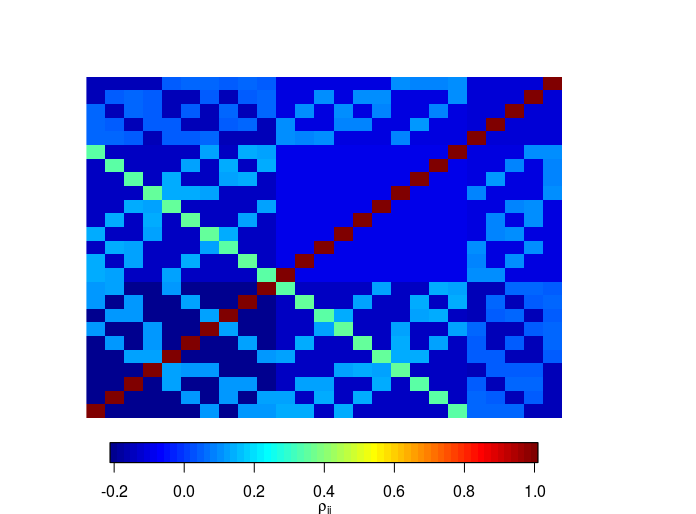
\includegraphics[scale=1]{\dir/figs/clade_corr.png} 
  \end{center}
\caption[Clade correlation matrix (coalescent prior), $n = 5$.]{\textbf{Clade correlation matrix (coalescent prior), $n = 5$}.
I sampled 10, 000 trees under the constant population size coalescent prior with contemporaneous tips using BEAST and computed the correlation matrix between clades of sizes between $2$ and $4$.
To facilitate visualisation of the structure in the matrix, I sorted clades by size (grows from bottom to top and left to right).
}
\label{fig:clade_corr}
\end{figure}


\subsection{Multi-dimensional scaling}
\label{sec:mds}

One way of visualising phylogenetic space is by employing lower-dimension projections that attempt to embed it in Euclidean space.
A very popular technique for this purpose is multi-dimensional scaling (MDS, \cite{Hillis2005}) of phylogenetic distances, in which the idea is to construct a new space with a few (usually two) dimensions that captures most of the features (variability) of the original space.
Suppose $\boldsymbol D$ is a phylogenetic distance matrix $D_{ij}$ is the distance -- under a particular distance $d_\sigma$ -- between two  phylogenies $i$ and $j$.
MDS proceeds by finding points $\boldsymbol x = \{x_1, x_2, \ldots, x_P\}$ such that a~\textbf{stress function}~\citep{Kruskal1964}\footnote{Other stress functions are possible, I keep the Kruskal-1 function here for simplicity and comparability with~\cite{Hillis2005}.}:
\begin{equation}
 \label{eq:stressF}
 S_D(\boldsymbol x) =  \sqrt{ \sum_{i \neq j = 1}^P \left( D_{ij} - |x_i - x_j|\right)^2},
\end{equation}
is minimised.
As pointed out by~\cite{Hillis2005}, under certain conditions this ensures the new space does not contain large distortions from the distance matrix and hence the new space can be used as representation of phylogenetic space.
Once we have an optimal solution computed from the observed distances, $\boldsymbol x$, we can use it to produce visualisations.

While the original paper by~\cite{Hillis2005} employed Robinson-Foulds to compose $\boldsymbol D$,~\cite{Jombart2017} generalise that approach by developing an R package to aid MDS visualisation under different metrics, with special focus on the KC metric~\citep{Kendall2016}.
In addition,~\cite{Jombart2017} also provide ways of extracting representative trees from a large sample, which reflect median points around which trees cluster.
This might prove particularly useful when finding and characterising \textit{modes} in phylogenetic space.

In order to enable meaningful comparisons between runs, I employ the Procrustes method to obtain an optimal rotation/scaling of the resulting distance matrices such that they are as compatible as possible. 
This helps minimise distortions caused by stochastic variation and allows MDS projections from different sets of phylogenies to be overlaid for comparison.
I used the function \verb|procrustes()| from the R package \textbf{vegan}~\citep{Oksanen2018} to obtain Procrustes-transformed matrices.

\textbf{Limitations}

As noted in Section 3 of~\cite{Willis2017}, phylogenetic space cannot be completely embedded in Euclidean space, hence any procedure that produces a mapping $\boldsymbol\Phi \to \mathbb{R}^P$ will invariably lead to the loss of some information.
A comprehensive assessment of the relative merits of different stress functions and phylogenetic metrics is lacking, and unfortunately outside the scope of this chapter.
Moreover, since 2-d visualisations are so much easier to understand, practitioners might be tempted to only consider the first two coordinates of the transformed space, what might in turn lead to missing important features in the data.

\subsection{Graph (network) analysis of tree space}
\label{sec:graph}

Another useful way of representing the discrete (tree) component of phylogenetic space is equipping it with a metric $d_\sigma$ and constructing a graph $G_\delta(V_n, E_n)$ where each vertex corresponds to a tree topology and there is an edge between two edges (trees) if they are a distance $d_\sigma \leq \delta$ apart under the chosen metric.
Thus, for this ``meta-graph'', $|V_n| = |\boldsymbol T| = (2n-3)!!$ and $|E_n| \leq |V_n| (|V_n| - 1)/2$, although this last bound is very crude and can be refined for a given $d$ and $\delta$.
Common choices for metric include the nearest-neighbour interchange (NNI) and subtree prune-and-regraft (SPR) distances.
In particular,~\cite{Whidden2015} show how one can construct the SPR graph of a sample of trees and then use graph-theoretic tools to quantify exploration of phylogenetic space. 
Starting from a sample of trees $\boldsymbol \tau = \{\tau_1, \tau_2, \ldots, \tau_M\}$, the analysis pipeline proposed by~\cite{Whidden2015} can be summarised as follows:
\begin{enumerate}
 \setcounter{enumi}{-1} 
 \item Rank the elements in $\boldsymbol\tau$ by their posterior probability (frequency), creating a set $\boldsymbol \tau_{\text{top}}$, also determine the most probable tree, $\tau_{\text{max}}$;
 \item Keep only the $m = \text{min}(4096, |\boldsymbol\tau_{\text{top}}|)$ first elements;
 \item Compute the $m \times m$ matrix of SPR distances between the samples, $\boldsymbol D$, and construct a graph $\boldsymbol G$ where each tree is a vertex and two vertices $i$ and $j$ are connected by an edge if $D_{ij} = 1$, that is, if the two phylogenies are one SPR operation apart from each other;
 \item Identify clusters of high-probability trees by iteratively clustering trees until $K=8$ clusters are obtained;
 \item Visualise the resulting graph annotating the vertices with posterior probabilities and distance to the most probable (or mode) tree. 
\end{enumerate}

~\cite{Whidden2015} also propose three metrics -- which can all be computed with a single pass on $\boldsymbol\tau_{\text{top}}$ -- to quantify exploration of tree space:
\begin{enumerate}
 \item Mean access time (MAT): average number of iterations required to visit any two trees;
 \item Mean commute time (MCT): average number of iterations required to go from $\boldsymbol \tau_{\text{top}}$ to each of the other high probability trees and back;
 \item Round-trip cover time: starting from $\tau_{\text{max}}$, the average number of iterations necessary to visit each high probability tree and then return to the mode tree. 
\end{enumerate}

\textbf{Limitations}

One of the advantages of building $\boldsymbol G$ using SPR distances is that many of its theoretical properties are better studied~\citep{Whidden2017}.
On the other hand, focusing on SPR distances disregards branch lengths, which is not always desirable, specially when dealing with time-calibrated phylogenies (see below).
Perhaps a more serious flaw with the SPR-graph approach is that for large $n$,  each tree visited in the MCMC is likely to be unique, and hence one cannot construct $\boldsymbol \tau_{\text{top}}$ based on posterior frequencies.

\subsection{Effective sample size and potential scale reduction factor for phylogenies}
\label{sec:treeESS}

Recently, researchers have also extended the concepts of effective sample size (ESS) and potential scale reduction factor (PSRF) to tree topologies, taking advantage of the fact that these quantities are defined w.r.t. the L$^2$ in Euclidean space.
\cite{Lanfear2016} propose two ESS-like metrics:  (i) the topological \textbf{approximate ESS}, $n_{\text{eff}}^T$ and (ii) the \textbf{pseudo-ESS}, $n_{\text{eff}}^P$.
If we define $\tau_f$ to be a focal tree and let $\boldsymbol L = \{l_1, l_2, \ldots, l_M \}, \: l_i = d_\sigma(\tau_i, \tau_f)$, the pseudo-ESS is simply the ESS of $\boldsymbol L$  computed as defined above (Eq~\ref{eq:ESSb}).
In other words, this measure attempts to reduce phylogenies to a univariate continuous quantity for which the methods discussed in Section~\ref{sec:continuous} can be applied.
An advantage of this approach is that it admits any choice of metric $d_\sigma$, which in turn means one can use metrics that account for branch lengths and topology simultaneously.
A perhaps more principled approach is to try to directly estimate the autocorrelation spectrum for phylogenies.
Let $d$ be the squared distance between two independent phylogenies.
The expected value of $d$ with $N$ independent samples is $(N(N-1)/4N^2)d$ and we can estimate $N$ when our sample has $M$ sequential observations by noting that 
\begin{align}
\label{eq:topoApproxESS}
\frac{N(N-1)}{4N^2} = \frac{\sum_{i = 1}^{M-1} \sum_{k = 1}^{\text{min}(m, M-i)}f(k)  + \frac{1}{2}(M-m + 1)(M-m)d}{2M^2},&\\
N = \left[\frac{2\sum_{i = 1}^{M-1} \sum_{k = 1}^{\text{min}(m, M-i)}f(k)  + (M-m + 1)(M-m)d - M^2}{M^2}\right]^{-1},&
\end{align}
where $f(k)$ is the squared distance between two samples at sampling interval (lag) $k$ and $m$ is the minimum sampling interval at which any two samples are independent,~\textit{i.e.}, the point where the autocorrelation function reaches an asymptote.  
\cite{Lanfear2016} suggest using an exponential model to estimate the autocorrelations, $f_a(k) = d(1-\exp(k/a))$, where $a$ is a shape parameter.
Implementations of both these functions are available in the \textbf{RWTY} package~\citep{Warren2017}.

The idea of treating squared distances as a surrogate for variance as employed above can be further extended to compute a PSRF-like for multiple samples of phylogenies.
\cite{Whidden2015} propose a ``topological Gelman--Rubin-like convergence diagnostic'', $\hat{R}^\prime$, that is very similar to~(\ref{eq:PRSF}) with $B$ and $W$ replaced by:
\begin{align}
 W^\prime &= \left(M(M-1)\right)^{-1}\sum_{k =1}^K\sum_{j_1 = 1}^M\sum_{j_2 = 1}^M d_\sigma(\tau_{kj_1}, \tau_{kj_2})^2,\\
 B^\prime &= \left((K-1)KM^2\right)^{-1} \sum_{i_1 = 1}^K\sum_{i_2 = 1}^K\sum_{j_1 = 1}^M \sum_{j_2 = 1}^M d_\sigma(\tau_{i_1j_1}, \tau_{i_2j_2})^2,\: \text{hence}\\
 \label{eq:PSRF-phylo}
 \hat{R}^\prime &= \sqrt{\frac{ (M-1)W^\prime +  B^\prime }{MW^\prime}}.
\end{align}
As with the original PSRF, $\hat{R}^\prime$ approaches 1 as the $K$ independent runs converge, and $\hat{R}^\prime < 1.1$ cut-off for convergence could be adopted.

\textbf{Limitations}

According to~\cite{Lanfear2016}, the pseudo-ESS can be sensitive to the choice of focal tree.
While that could be remedied in principle by choosing, for instance, the maximum clade credibility (MCC) phylogeny as $\tau_f$, it is unclear to me what biases this could introduce.
The original formulation of~(\ref{eq:PSRF-phylo}) by~\cite{Whidden2015} considered only SPR distances, but this can be easily generalised to other distances that include branch lengths.
A minor point about these diagnostics is that due to their recent development in-depth theoretical and empirical studies are still lacking.
For instance, the choice of metric might play an important role in the power to detect convergence problems, but this aspect remains to be investigated.

\subsection{A word of caution}

As Charlie Geyer points out in the very quaintly named web page ``On the Bogosity of MCMC Diagnostics''\footnote{Available from \url{http://users.stat.umn.edu/~geyer/mcmc/diag.html}, accessed on 2018-02-18.}, all known diagnostic measures
%-- barring perhaps the so-called ``perfect sampling'' method~\citep{Propp1996} --
have serious shortcomings and, in his words, can detect only ``... obvious, gross, embarrassing problems that jump out of simple plots''.
While I do not completely subscribe to Geyer's view,  I agree that subtle problems such as small biases in the Hastings ratio (see e.g.~\cite{Holder2005}) or funnel-like effects of posterior (prior) correlation are likely to remain undetected.
Therefore a word of caution is warranted: even when one fails to detect convergence problems~\citep{Cowles1999}, they may very well still be present in the form of subtle biases, the impact of which on inferences drawn from the MCMC samples is hard to predict.

\section{Accommodating time-calibrated phylogenies}
\label{sec:accommodating}

In this Chapter I provide a first attempt at an unified workflow for Bayesian estimation of time-calibrated phylogenies (TCPs) with special focus on phylodynamic inference.
As discussed previously, TCPs are special objects in that the branch lengths are measured in units of calendar time.
In what follows I detail my investigations into several issues related to accommodating time-calibrated phylogenies and diagnosing the convergence of MCMC runs from BEAST.
Considering the methods currently available, the main difficulties faced when exploring the space of TCPs are:
\begin{itemize}
 \item Size: the phylogenies used in phylodynamic studies have $n$ of the order of hundreds to a few thousands (see below);
 \item Branch lengths: in time-calibrated phylogenies branch lengths are of crucial importance and hence cannot be ignored;
 \item Sampling structure: TCPs usually have serially-sampled tips/leaves.
 The distribution and range of the sampling times imposes constraints on the phylogenetic space, leading to ``rugged'' posterior distributions~\citep{Brown2018} -- see also Figure 3. in~\cite{Moller2018} and discussion therein. 
\end{itemize}

Most routines in AWTY are designed for unrooted trees and implicitly assume a relatively small number of taxa ($n < 50$).
Moreover, the MDS routines presented in~\cite{Hillis2005} and available in the~\textbf{RWTY} package use the Robinson-Foulds distance which does not capture branch length differences and hence is not appropriate for time-calibrated phylogenies if used in isolation.
The routines available in the~\textbf{RWTY} package also use RF as the default metric, and as far I am aware, the only metric that includes branch lengths available in the package is path distance (BS, see Section~\ref{sec:metrics}).
Here I relax this by including many other metrics (see below), for which the approximate ESS of~\cite{Lanfear2016} can be computed following equation~(\ref{eq:topoApproxESS}).
As the number of taxa grows, it gets progressively harder to track clades, both from a statistical and a computational point of view.
Computationally, it becomes cumbersome to compute indicators for all clades in a run, in addition to plotting clade frequencies.
This latter problem can be tackled by only paying attention to clades with a particular (posterior) frequency.
Statistically, however, the space of clades presents some non-trivial correlation structure that might make it hard to obtain reliable global indicators of convergence and mixing.
In Section~\ref{sec:cladeSwitch}, I provide a more detailed discussion of these issues.
Nonetheless, in the interest of consistence and comparability with previous approaches I include diagnostics of convergence and mixing in clade space. 

In a phylodynamic analysis context one may be chiefly interested in a set $\boldsymbol\theta^\star$ parameters, which might include quantities such as the reproductive ratio $R_0$~\citep{Stadler2011} or the wave front velocity of an epidemic~\citep{Lemey2010,Pybus2012}.
It is therefore important to study the behaviour of the chains for $\boldsymbol\theta^\star$, as well as account for the correlations between parameters.
Fortunately, there are a plethora of tools designed to diagnose convergence for continuous parameters, many of which are available in the R package~\textbf{coda}~\citep{Plummer2006} and the GUI application Tracer~\citep{Rambaut2018}.

The pipeline/workflow proposed here can be summarised as follows:
\begin{enumerate}
 \item Run (at least) three independent chains for $M$ iterations each, keeping $M_t$ phylogenies;
 \item Compute univariate ESS, PSRF and mESS for $\boldsymbol\theta^\star$;
 \item (Sub)sample a number $K < M_t$ of trees and compute ($ K \times K$) distance matrices under different metrics;
 \item Perform MDS on the distance matrices and use them to visualise phylogenetic space (see Figure~\ref{fig:pipeline}b);
 \item Using the same distance matrices, compute the approximate ESS~\citep{Lanfear2016} for each run under different metrics;
 \item Compute clade frequencies and indicator matrices and calculate clade ESS, clade switching and average standard deviation in split/clade frequencies (ASDSF);
\end{enumerate}

\subsection*{Specialised computer programs}

Most modern phylodynamic studies include data sets with hundreds to a few thousands of samples (taxa) and the resulting phylogenies strain the capacity of most existing packages (including AWTY and RWTY).
Computationally, one of the main bottlenecks is loading trees into memory -- which is quite slow in R, for instance.
I instead do the tree-processing externally using specialised classes in BEAST (\verb|dr.app.tools.TopologyTracer|)\footnote{Implemented by Andrew Rambaut and Guy Baele (Leuven) with input and testing from me.}, controlled using simple bash scripts.
I then wrote custom R functions to transform the output of \verb|TopologyTracer| so that it could be analysed using heavily modified functions in the package~\textbf{RWTY}~\cite{Warren2017}.
The same strategy can be adopted when processing clade frequencies: I used the class \verb|dr.app.tools.TreeSummary| to compute clade frequencies and construct the indicator matrix and then modified functions from the \textbf{RWTY} package for plotting and presenting the results.
As mentioned above, I employ the packages~\textbf{mcmse}~\citep{Flegal2017} and~\textbf{coda}~\citep{Plummer2006} to compute (univariate and multivariate) effective sample sizes and potential scale reduction factors for continuous parameters.
This is done to keep all computations contained in the R environment, which allows the whole workflow to be encapsulated into a (R)Markdown document which can be rendered to html and/or PDF (see Figure~\ref{fig:pipeline}).
A suite of R and bash scripts -- as well as the RMarkdown report --  to perform these tasks is available from~\url{https://github.com/maxbiostat/BEAST_convergence_pipeline}\footnote{If these functions prove to be sufficiently useful to other researchers, I may build an R package.}.
For convenience, the analysis of the ``poor'' runs is included in Appendix A as an example.
\begin{figure}[!ht]
\begin{center}
  \subfigure[\textbf{Continuous parameters}]{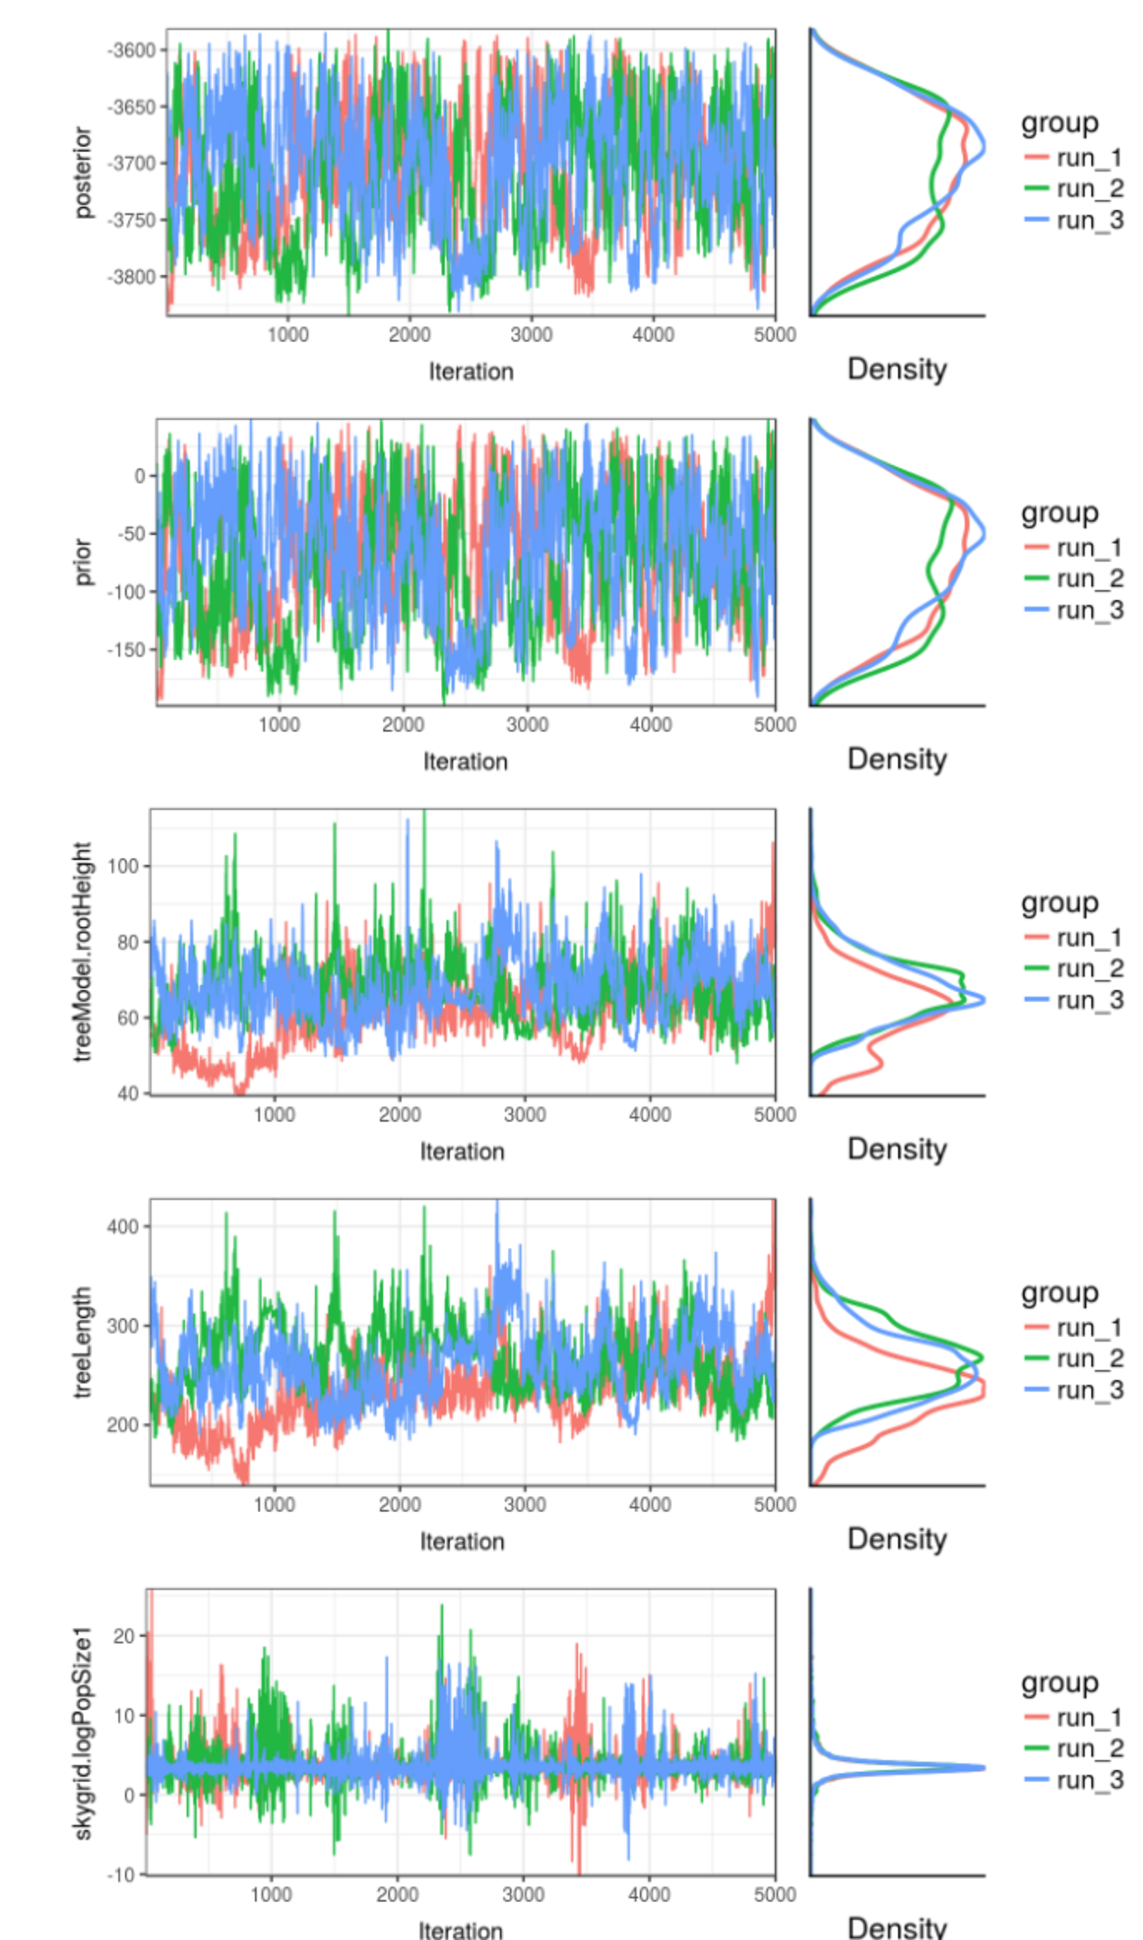
\includegraphics[scale=0.35]{\dir/figs/pipeline_screenshot.pdf}}%
  \subfigure[\textbf{MDS}]{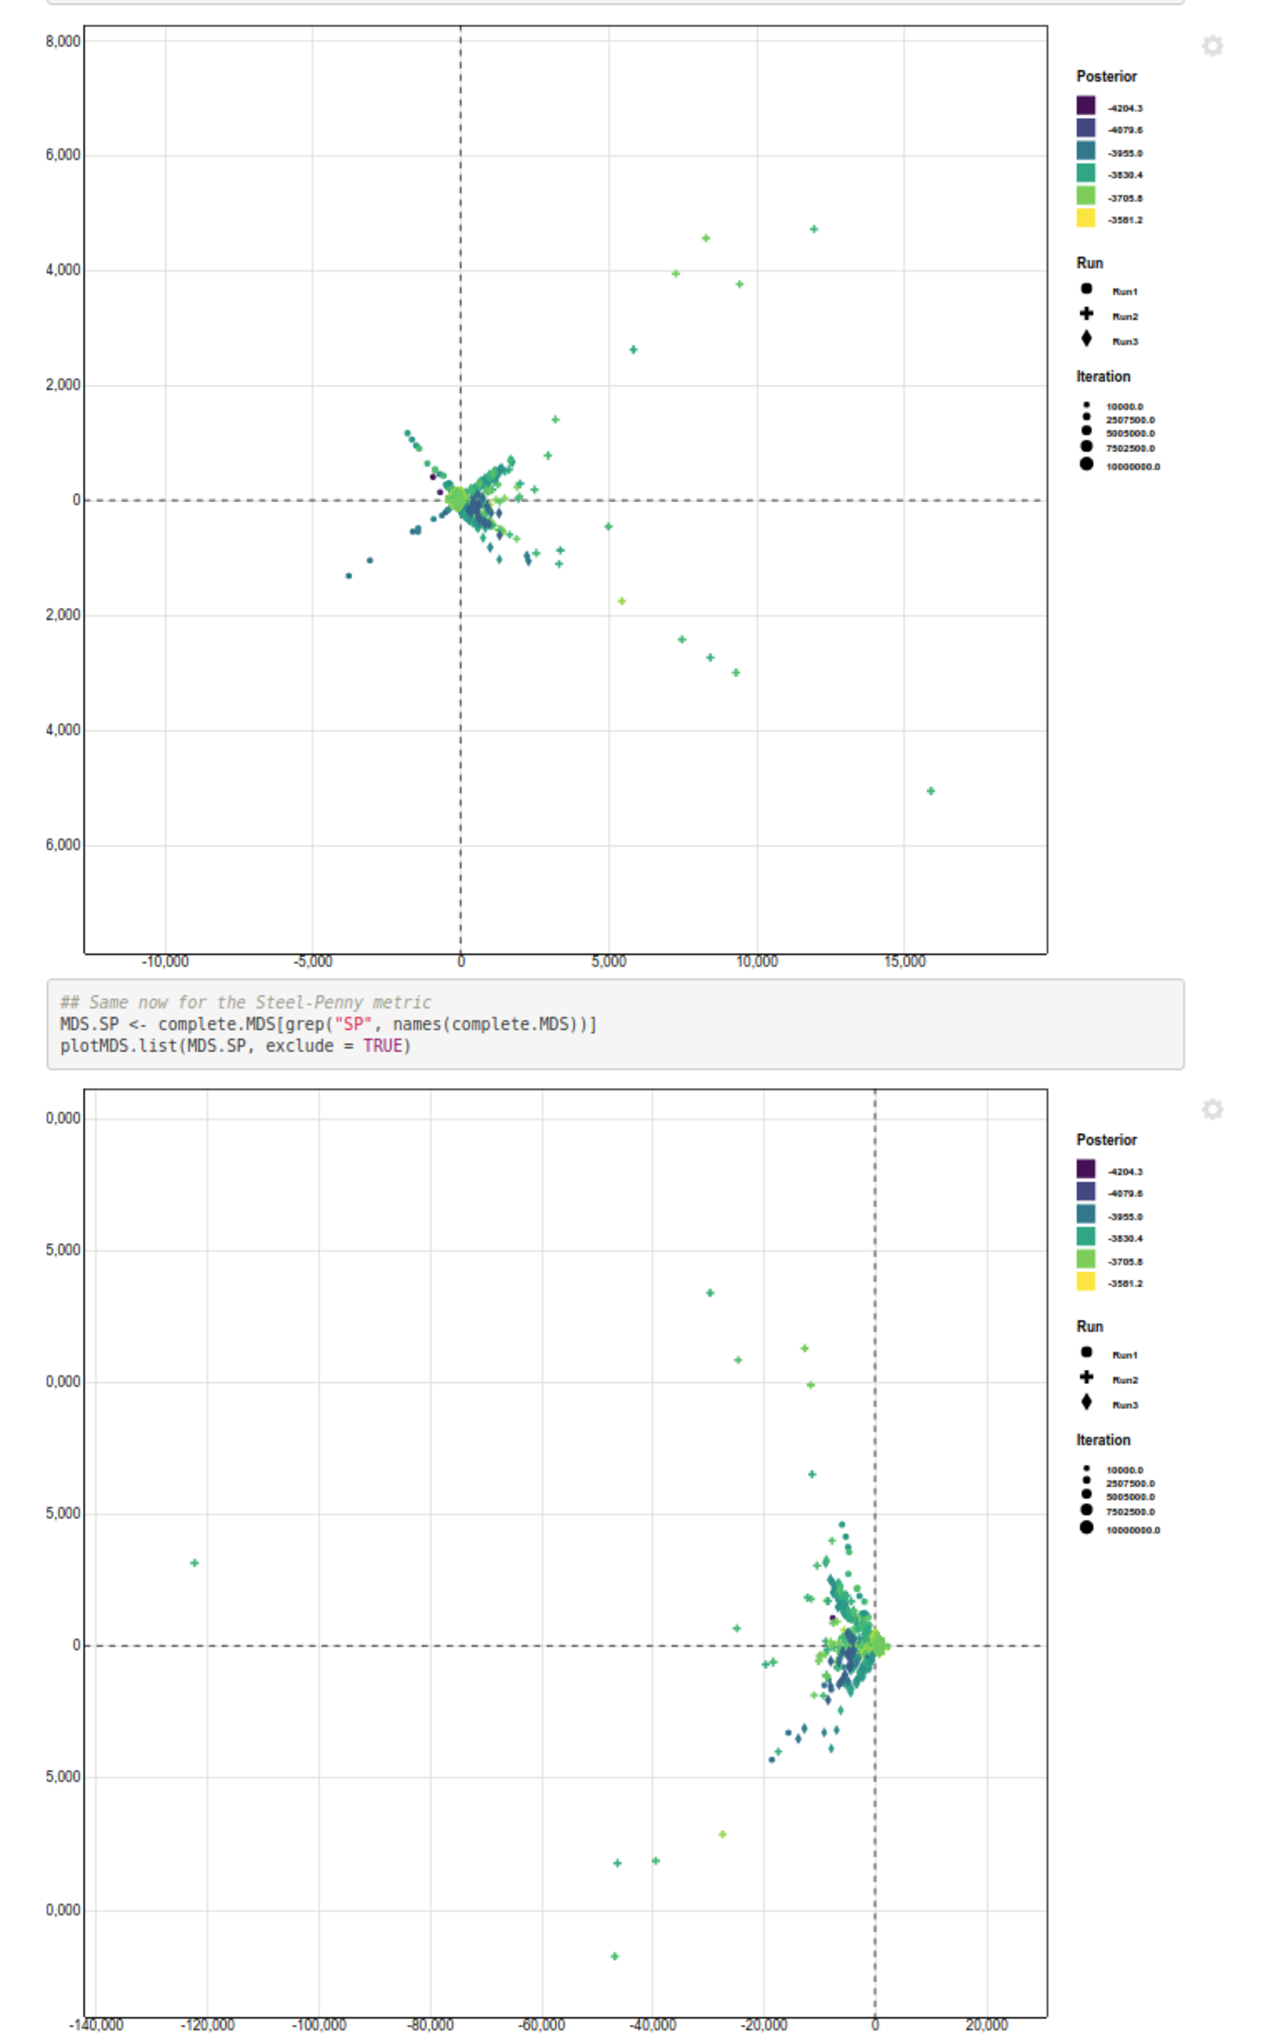
\includegraphics[scale=0.35]{\dir/figs/pipeline_screenshot_mds.pdf} } 
\end{center}
 \caption[Screen capture of the proposed MCMC diagnostics pipeline.]{\textbf{Screen capture of the proposed MCMC diagnostics pipeline}.
One can check  trace plots -- as well as investigate univariate and multivariate ESS -- for continuous parameters (a) and study exploration of phylogenetic space by visualising MDS (b) -- note these latter plots are made interactive  using the spreadD3() function in R.
All routines have been written in R and organised into an RMarkdown document that generates an html report that can easily explored by the user to diagnose problems with her MCMC runs.
See Appendix A for more.
 }
 \label{fig:pipeline}
\end{figure}

\section{Data sets}
\label{sec:data}

Here I will analyse the same data sets described in Table~\ref{tab:datasets} in Chapter 2.
In particular, \verb|Dengue4|, due to its manageable size but relatively high complexity (multiple partitions, temporal structure, etc), will be used to exemplify the full breadth of convergence diagnostics available and how they may be combined for maximum efficacy.
I will analyse MCMC runs resulting from empirical analyses of these data sets to investigate the characteristics of phylogenetic space for serially-sampled data modelled under phylodynamic models.
For the results in Section~\ref{sec:combining}, I constructed a deliberately bad MCMC sampler to obtain a poorly mixing chain.
To achieve this I employed only the \verb|WideExchange| operator  -- with small weight -- to sample tree topologies.
Since this operator is not "tunable" and has a very low acceptance probability ($0.021$ for this data set), the chain mixes poorly.
These poorly mixing (Poor) runs were then compared with runs using the default settings in BEAUti, the GUI configuration file maker for BEAST.
In addition, I ran the pipeline with \verb|STL| replacing all tree-related operators with the \verb|SubTreeLeap| operator described in Chapter 2.
All runs had 10 million iterations and a thinning interval of a thousand states. 

\subsection{Simulated data}
\label{sec:simudata}

I also created a simulated data set to have a baseline where we know the ground truth.
I first obtained a 50 taxa subtree with uniformly temporally sampled tips from a larger EBOV phylogeny~\citep{Dudas2017}, henceforth called ``empirical tree''.
To assess the effect of tree shape, I simulated a coalescent tree with the same tip-date sampling structure under a constant population model with $N_e = 10$, which I will call ``coalescent tree''.
I then simulated alignments of 1,000, 5,000 and 10,000 sites down both trees with a substitution rate of $10^{-3}$ substitutions per site per year, generating 6 alignments.
For each alignment, I then ran three independent runs (replicates) of both STL and the default/classic mix.
To explore convergence times and obtain more stable estimates of the posterior, each combination of data set and transition kernels was run 10 million and 100 million iterations.

\section{Analysis}
\label{sec:results}

\subsection{Combining diagnostic measures}
\label{sec:combining}

The first set of results I will present is the development of an analysis ``pipeline'' for MCMC diagnostics in Bayesian phylogenetics.
In particular, I will use the Dengue serotype 4 \textit{env} (\verb|Dengue4|) -- 17 taxa, 1485 sites -- to showcase how many convergence diagnostic measures can be employed in conjunction as part of the Bayesian phylogenetic workflow.
Appendix A shows the analysis of the poorly mixing runs using the steps and computer programs described above.
In this section I focus on comparing some results for three MCMC schemes: poorly mixing, default settings and \verb|STL|.

First, I present the results of convergence diagnostics for continuous parameters, usually obtained with the graphical tool Tracer in the context of BEAST analyses.
Here however I compute some additional quantities not available in Tracer, such as multivariate ESS and potential scale reduction factor (PSRF).
Results in Table~\ref{tab:continuous_results} show that the poor runs have low univariate ESSs for continuous parameters highly dependent on the tree (e.g., mean evolutionary rate, \verb|meanRate|), whereas ESS are in the low thousands for parameters such as the transition transversion rate ($\kappa$).
For this particular experiment and with no optimisation, \verb|STL| shows comparable if slightly inferior performance when comparing raw univariate ESSs.
The PSRFs show that for many of these parameters the three independent runs do not converge to the same point (PSRF $> 1.1$), be it individually for each parameter or globally across parameters (multivariate PSRF $> 1.1$).
While the \verb|STL| runs seem more consistent, as indicated by the slightly lower PSRFs, with only three runs (chains) per MCMC scheme this difference cannot be reliably established (see Chapter 2 for more thorough comparisons).
The multivariate ESSs might at first glance give the impression of good performance, but in fact all of them fall well short of the minimum ESS required for reliable inference (see caption in Table~\ref{tab:continuous_results}).
Notice that while this is specially the case for the poor runs (as expected), none of the runs across MCMC schemes achieve the minimum ESS (8831) after 10 million iterations (see Discussion).

\begin{sidewaystable}[!ht]
\caption[Convergence diagnostics for continuous parameters.]{\textbf{Convergence diagnostics for continuous parameters}.
I show the summary convergence diagnostics from the pipeline described in Section~\ref{sec:accommodating} for three MCMC schemes, running three chains for each.
$^1$ - First (log) population  from Skygrid.
$^2$ - The ratio between the average rate and the standard deviation of rates across all branches.
$^3$ - Covariance between rate assignments in the tree.
$^4$ - Multivariate ESS as in~\cite{Vats2015} and multivariate potential scale reduction factor (PSRF).
The minimum multivariate ESS for all parameters considered is $8831$ according to the formula in~(\ref{eq:mESSbound}).
}
\label{tab:continuous_results}
\begin{center}
\small\addtolength{\tabcolsep}{-5pt}
 \begin{tabular}{ccccc|cccc|cccc}
\toprule
                         & \multicolumn{4}{c}{Poor}                  & \multicolumn{4}{c}{Default}               & \multicolumn{4}{c}{STL}                   \\
\midrule                         
Parameter                & ESS 1 & ESS 2 & ESS 3 & PSRF        & ESS 1 & ESS 2 & ESS 3 & PSRF        & ESS 1 & ESS 2 & ESS 3 & PSRF        \\
\midrule
Tree height              & 57      & 40      & 13      & 1.11 (1.33) & 1063    & 1113    & 876     & 1.03 (1.10) & 858     & 937     & 940     & 1.00 (1.01) \\
Tree length              & 55      & 34      & 7       & 1.17 (1.49) & 1021    & 1150    & 907     & 1.03 (1.10) & 860     & 1373    & 907     & 1.00 (1.01) \\
(log) Pop Size$^1$           & 622     & 657     & 27      & 1.01 (1.02) & 1098    & 833     & 751     & 1.00 (1.01) & 230     & 1138    & 1261    & 1.02 (1.03) \\
CP1.alpha                & 7446    & 6992    & 7202    & 1.00 (1.00) & 2705    & 2659    & 2484    & 1.00 (1.01) & 3567    & 3377    & 3320    & 1.00 (1.00) \\
CP1.kappa                & 8620    & 8695    & 8640    & 1.00 (1.00) & 4360    & 3796    & 3753    & 1.05 (1.07) & 5204    & 5551    & 4912    & 1.00 (1.00) \\
CP2.kappa                & 6763    & 6876    & 7325    & 1.00 (1.00) & 2674    & 2807    & 1983    & 1.00 (1.01) & 3255    & 3761    & 3571    & 1.00 (1.00) \\
Mean rate                & 46      & 49      & 12      & 1.17 (1.49) & 1058    & 1270    & 846     & 1.00 (1.00) & 741     & 1396    & 1002    & 1.00 (1.01) \\
Coefficient of variation$^2$ & 26      & 41      & 7       & 1.12 (1.28) & 748     & 794     & 817     & 1.00 (1.00) & 531     & 1147    & 1178    & 1.01 (1.02) \\
Covariance$^3$               & 3370    & 3370    & 1315    & 1.00 (1.00) & 5168    & 5209    & 5134    & 1.00 (1.00) & 6148    & 6088    & 6124    & 1.00 (1.00) \\
Multivariate ESS/PSRF$^4$    & 1299    & 1212    & 937     & 1.13        & 2018    & 2170    & 2034    & 1.02        & 1808    & 2632    & 2407    & 1.01       \\
\bottomrule
\end{tabular}
\end{center}
\end{sidewaystable}

Considering mixing and convergence in phylogenetic space through the use of specially tailored diagnostics presented in Table~\ref{tab:tree_results}, shows that while the approximate ESS~\citep{Lanfear2016} does capture major differences in mixing, it is inconsistent, both within and between metrics.
As an example, take the tree ESS with the Steel-Penny (SP) metric for the Poor runs: for one of the chains, it achieves its maximum value of 1001, when it clearly cannot be the case that the sample comprised 1001 independent samples considering all available evidence.
The clade switching score (CSS) and mean ESS for clade indicators seem to discriminate well between the Poor runs and the default (and \verb|STL|) ones.
ASDSF is also above the common threshold of $0.10$ used for convergence~\citep{Ronquist2012}; \verb|STL| seems to lead to slightly better performance according to this metric.
\begin{sidewaystable}[!ht]
\begin{center}
 \centering
\caption[Convergence diagnostics in phylogenetic space.]{\textbf{Convergence diagnostics in phylogenetic space}.
I show convergence diagnostics specially tailored towards phylogenetic space, such as the approximate ESS of~\cite{Lanfear2016} (for various metrics), the average univariate ESS for clade indicators$^1$, the clade switching score$^2$ and the average standard deviation in split/clade frequencies$^3$.
Tree ESSs computed using a sample of $1001$ trees following the expression in~(\ref{eq:topoApproxESS}).
}
\label{tab:tree_results}
\begin{tabular}{cccc|ccc|ccc}
\toprule
                 & \multicolumn{3}{c}{Poor}    & \multicolumn{3}{c}{Default} & \multicolumn{3}{c}{STL}     \\
                 \midrule  
                 & Chain 1 & Chain 2 & Chain 3 & Chain 1 & Chain 2 & Chain 3 & Chain 1 & Chain 2 & Chain 3 \\
                 \midrule  
Tree ESS (KC, $\lambda = 0$)   & 33      & 38      & 39      & 743     & 1001    & 1001    & 523     & 734     & 465     \\
Tree ESS (KC, $\lambda = 1/2$) & 156     & 305     & 20      & 444     & 581     & 1001    & 292     & 231     & 445     \\
Tree ESS (KC, $\lambda = 1$)   & 139     & 395     & 19      & 371     & 705     & 711     & 276     & 276     & 1001    \\
Tree ESS (RF)    & 55      & 114     & 36      & 794     & 1001    & 801     & 695     & 624     & 787     \\
Tree ESS (SP)    & 66      & 1001    & 14      & 403     & 659     & 659     & 184     & 155     & 552     \\
Tree ESS (CD)    & 1001    & 431     &  87     & 1001    & 1001    & 1001    & 1001    & 1001    & 1001     \\
Tree ESS (BS)    & 212     &  259    &  25     & 260     & 445     & 675     & 232     & 241     & 340     \\
Mean clade ESS$^1$   & 874     & 917     & 837     & 7321    & 7446    & 7420    & 7506    & 7477    & 7428    \\
CSS$^2$              & 0.16    & 0.18    & 0.16    & 0.87    & 0.88    & 0.88    & 0.88    & 0.88    & 0.9     \\
ASDSF$^3$            & 0.18    & 0.39    & 0.29    & 0.08    & 0.09    & 0.04    & 0.05    & 0.03    & 0.04   \\
\bottomrule
\end{tabular}
\end{center}
\end{sidewaystable}

I now move on to explore some more specific questions about phylogenetic space and its representations.

\subsection{Representation of phylogenetic space under different metrics}
\label{sec:representation}

While multi-dimensional scaling can be useful for visualising phylogenetic space, the issue of which metric to employ remains.
Since each of the many available metrics capture distinct features, one has to analyse MDS projections under different metrics in order to have a better grasp of the geometry of phylogenetic space.
In Figure~\ref{fig:mds_ebov_RF} I show the MDS projection of Robinson-Foulds (RF) distances between MCMC samples for the large Ebola virus data set (\verb|EBOVa|) -- the analysis detailed in Chapter 2, see Figure~\ref{fig:ebovmultimod}. 
It is clear that run 3 for the \verb|STL| operator (see Chapter 2) is distinct from the others. 
In addition, one can see that the last samples of run 2 \verb|STL| (larger green points) are closer to the region visited by the default runs and \verb|STL| run 1.
These results show that the projection using the Robinson-Foulds capture important features of phylogenetic space, leading to clearly separated clusters of trees with different likelihoods.

\begin{figure}[!ht]
\begin{center}
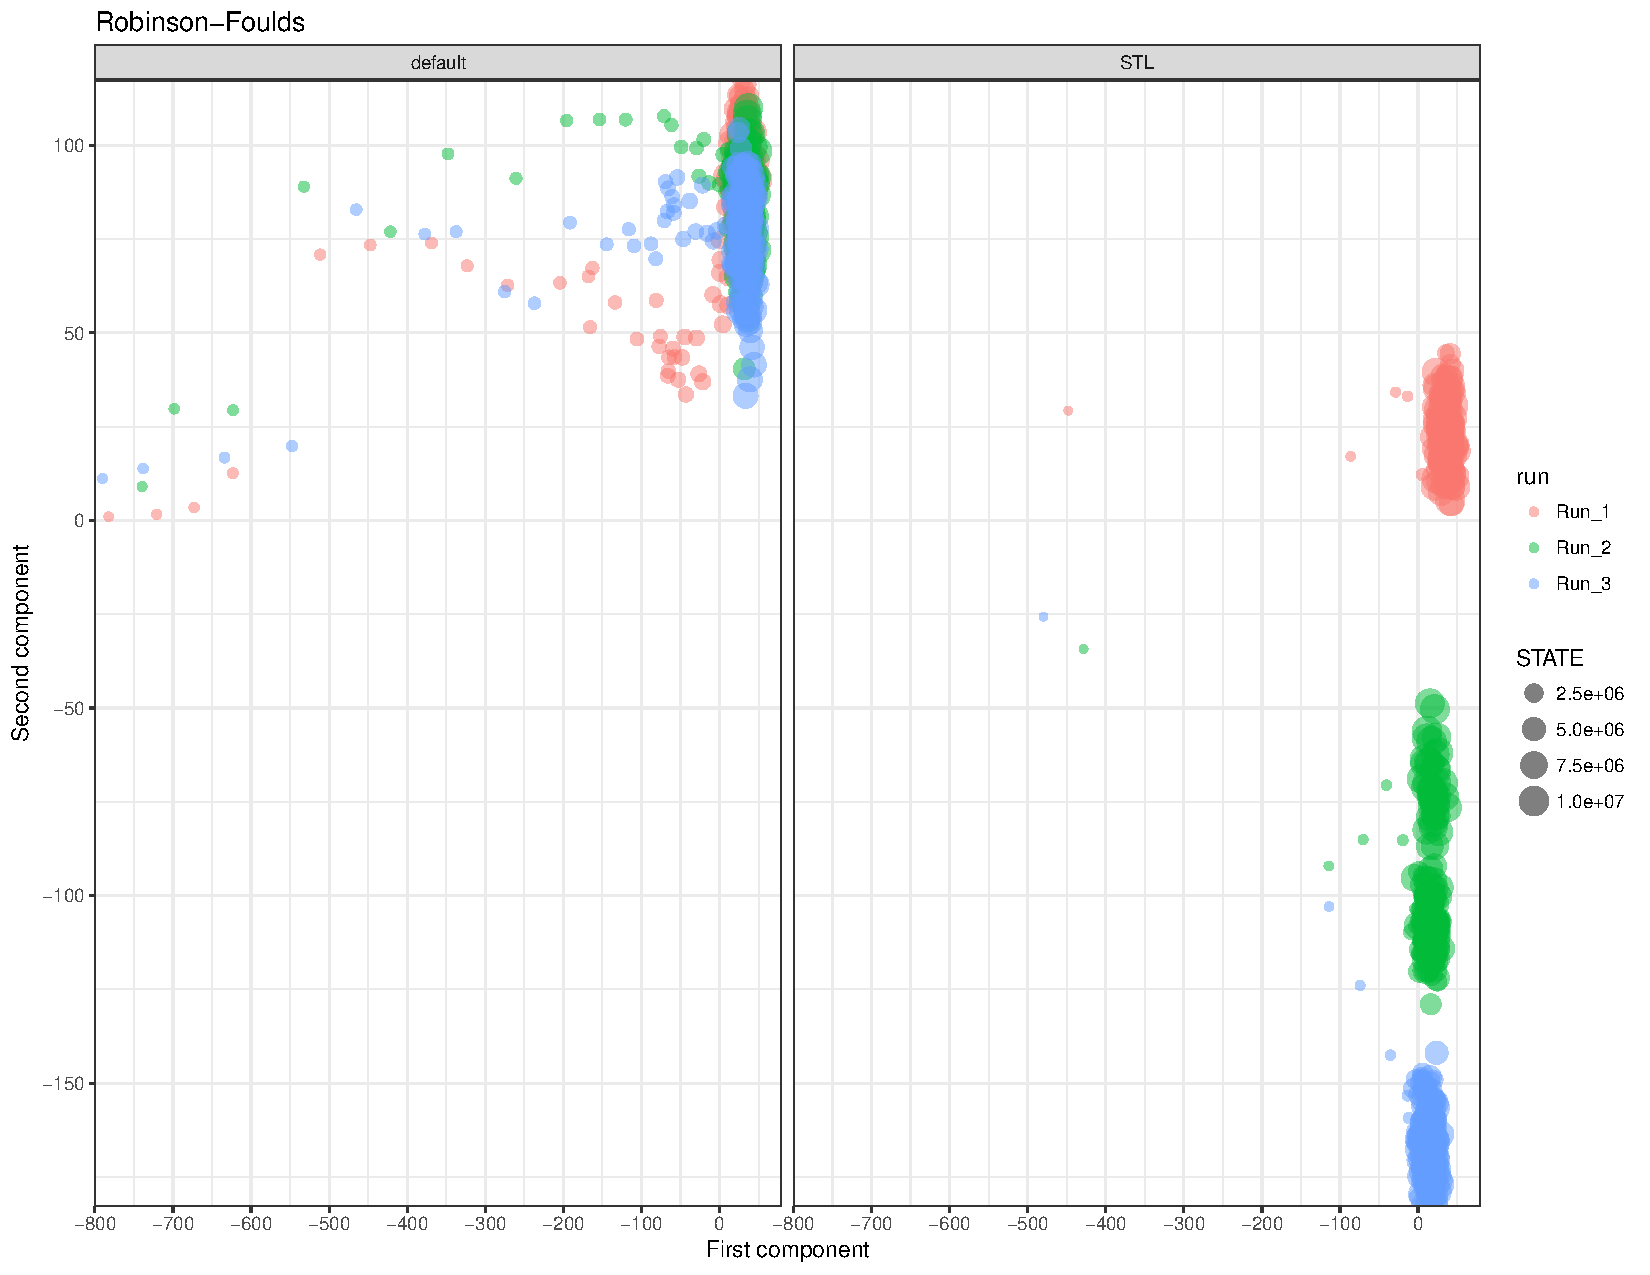
\includegraphics[scale=0.5]{\dir/figs/mds_ebov_RF.pdf} 
\end{center}
 \caption[MDS projections for the full EBOV 1610 taxa data set (Robinson-Foulds distances).]{\textbf{MDS projections for the full EBOV 1610 taxa data set (Robinson-Foulds distances).}
 I sampled 200  equally spaced trees from each chain (1200 trees in total) and computed the Robinson-Foulds distance~\citep{Robinson1981} for every pair of trees.
 Colours relate to the seed used in the pseudo random number generator, ensuring each run starts from the same point. 
 Please see Figure~\ref{fig:ebovmultimod} in Chapter 2 for more details. 
 }
 \label{fig:mds_ebov_RF}
\end{figure}

Importantly, however, these differences are not captured by other metrics.
The projections under the Kendall-Colijn  (KC) metric in Figure~\ref{fig:mds_ebov_KC} shows no obvious clustering of the runs, even though we know different runs explore trees with very different likelihoods.
In panel (a), I show the MDS projection of KC metric  with $\lambda = 0$, that considers only topological differences between phylogenies, but the projections do not show any obvious clustering of the runs, unlike the RF metric (Figure~\ref{fig:mds_ebov_RF}).
The projection with $\lambda = 1/2$ in panel (b) displays the same pattern.
This seems to suggest that MDS under this metric does not allow one to visualise the different modes in phylogenetic space, or, in other words, that KC is too smooth to capture the differences, at least for this data set.

\begin{figure}[!ht]
\begin{center}
\subfigure[$\lambda = 0$]{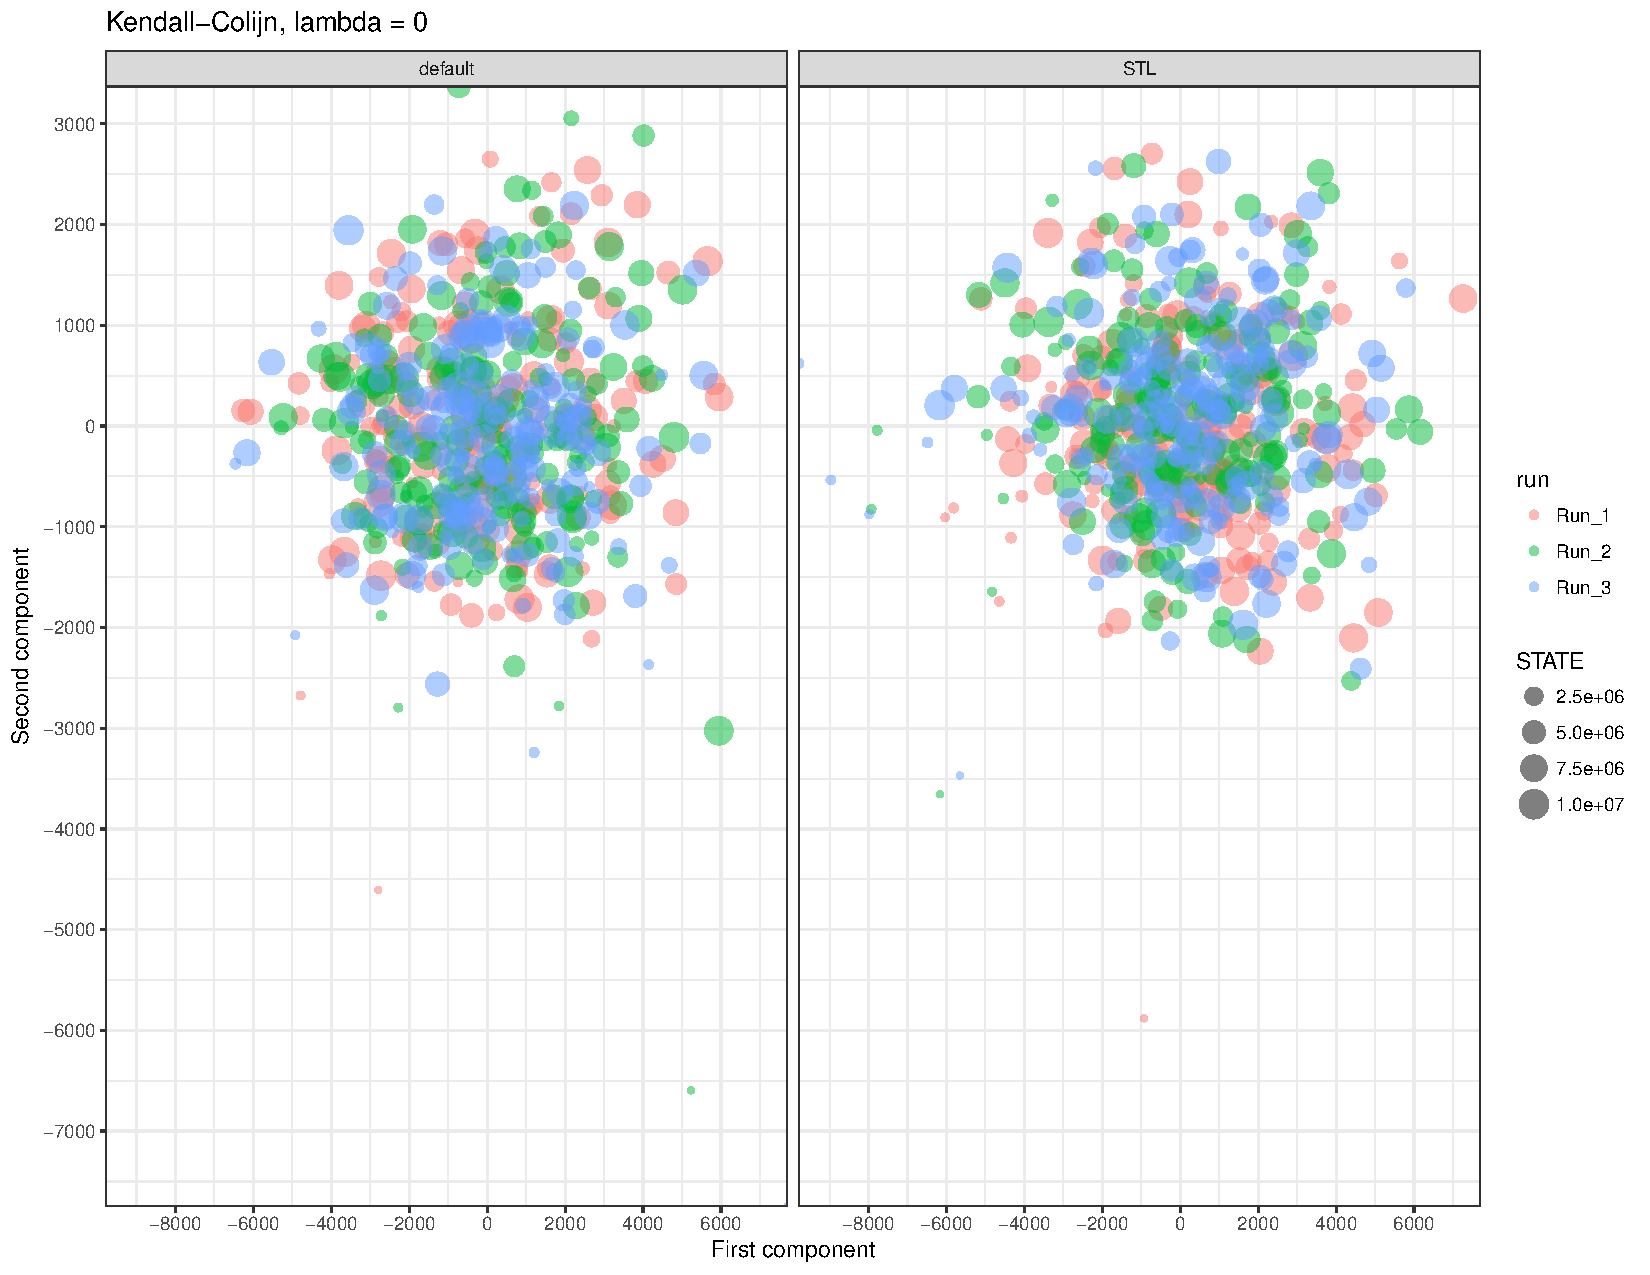
\includegraphics[scale=0.35]{\dir/figs/mds_ebov_KC0.pdf}}\\
\subfigure[$\lambda = 1/2$]{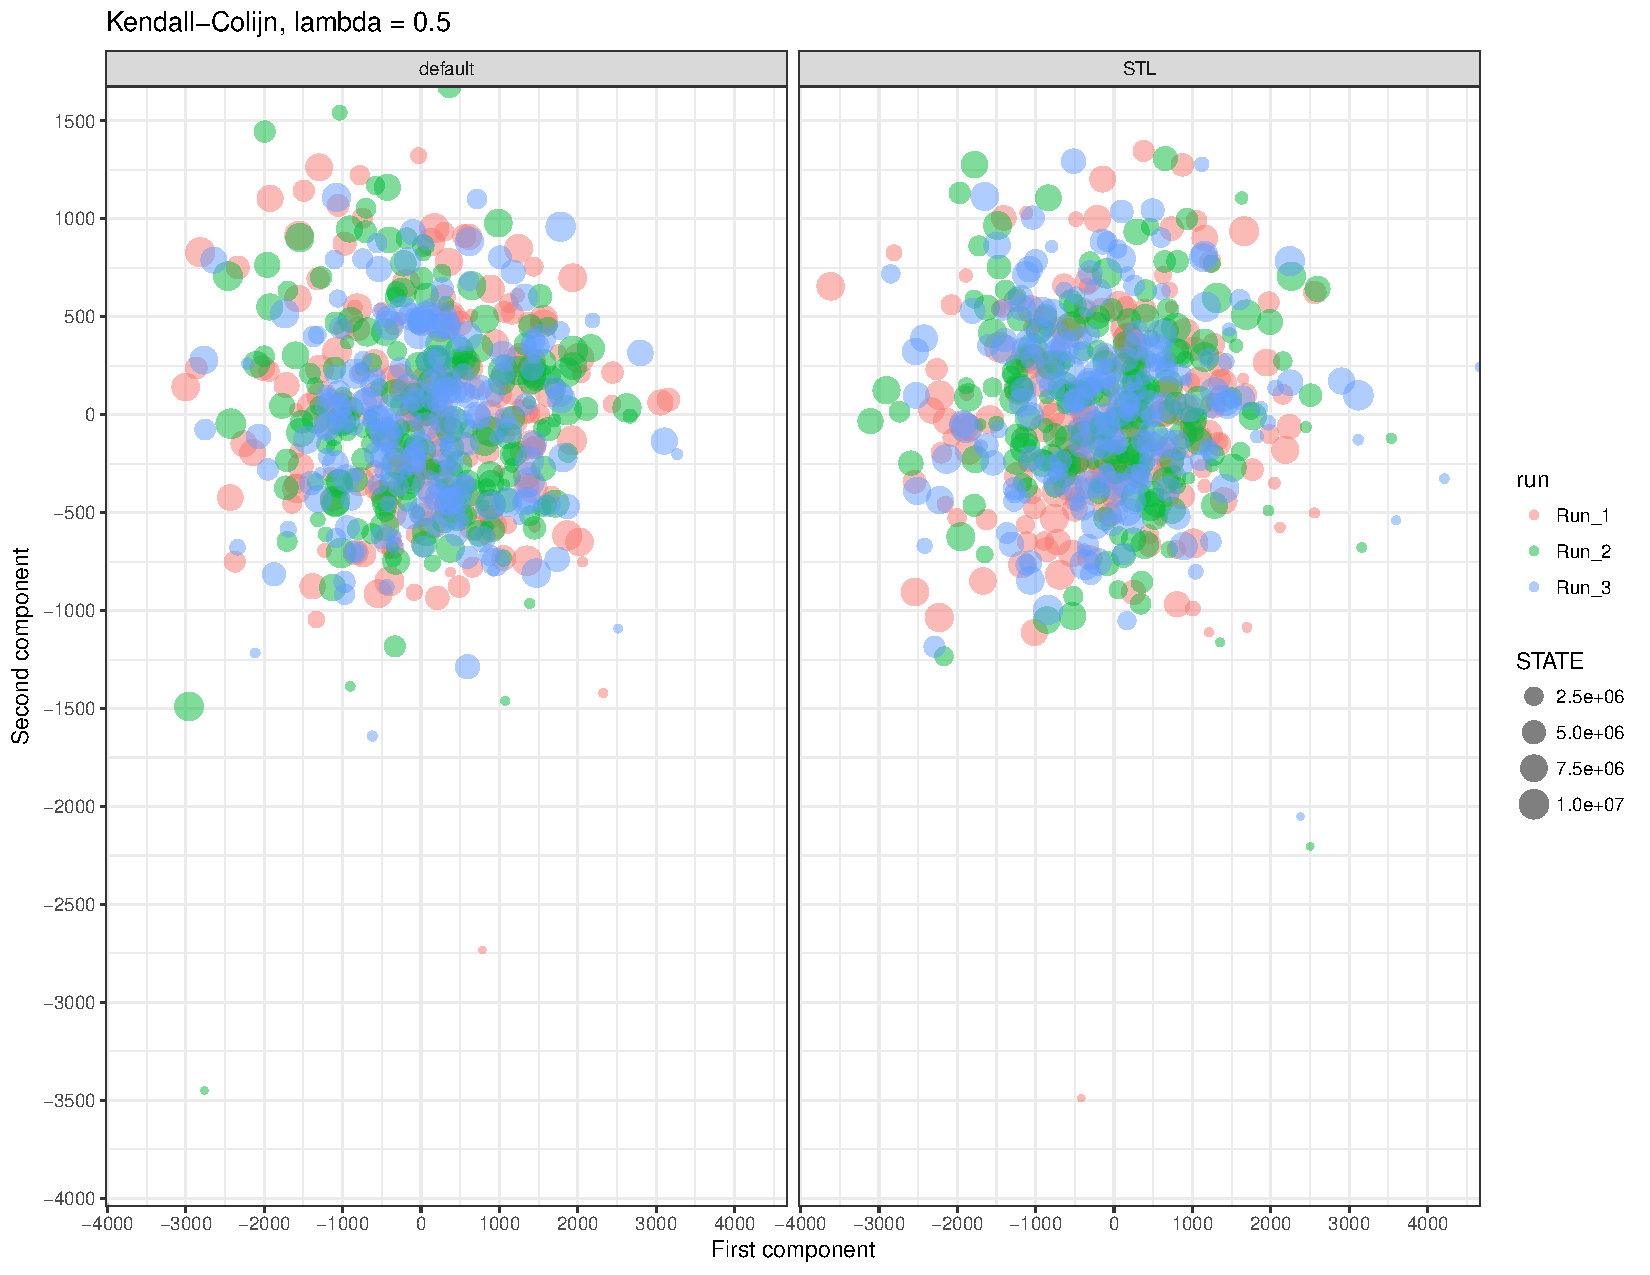
\includegraphics[scale=0.35]{\dir/figs/mds_ebov_KChalf.pdf}}
\end{center}
 \caption[MDS projections for the full EBOV 1610 taxa data set (Kendall-Colijn distances).]{\textbf{MDS projections for the full EBOV 1610 taxa data set (Kendall-Colijn distances).}
 I sampled 200 equally spaced trees from each chain (1200 trees in total) and computed the Kendall-Colijn distance with $\lambda = 0$ and $\lambda = 1/2$.
 Colours relate to the seed used in the pseudo random number generator, ensuring each run starts from the same point.  
 See Figure~\ref{fig:mds_ebov_RF} for the projection of the same trees under the Robinson-Foulds metric~\citep{Robinson1981}.
 }
 \label{fig:mds_ebov_KC}
\end{figure}

In Figure~\ref{fig:mds_ebov_SP} we can again notice the lack of differentiation between the runs, suggesting the SP metric shares the ``smoothness''  displayed by the KC metric.
Taken together, these results suggest that great care needs to be taken when visualising phylogenetic space because important features might not be easy to distinguish under many (most) metrics.

\begin{figure}[!ht]
\begin{center}
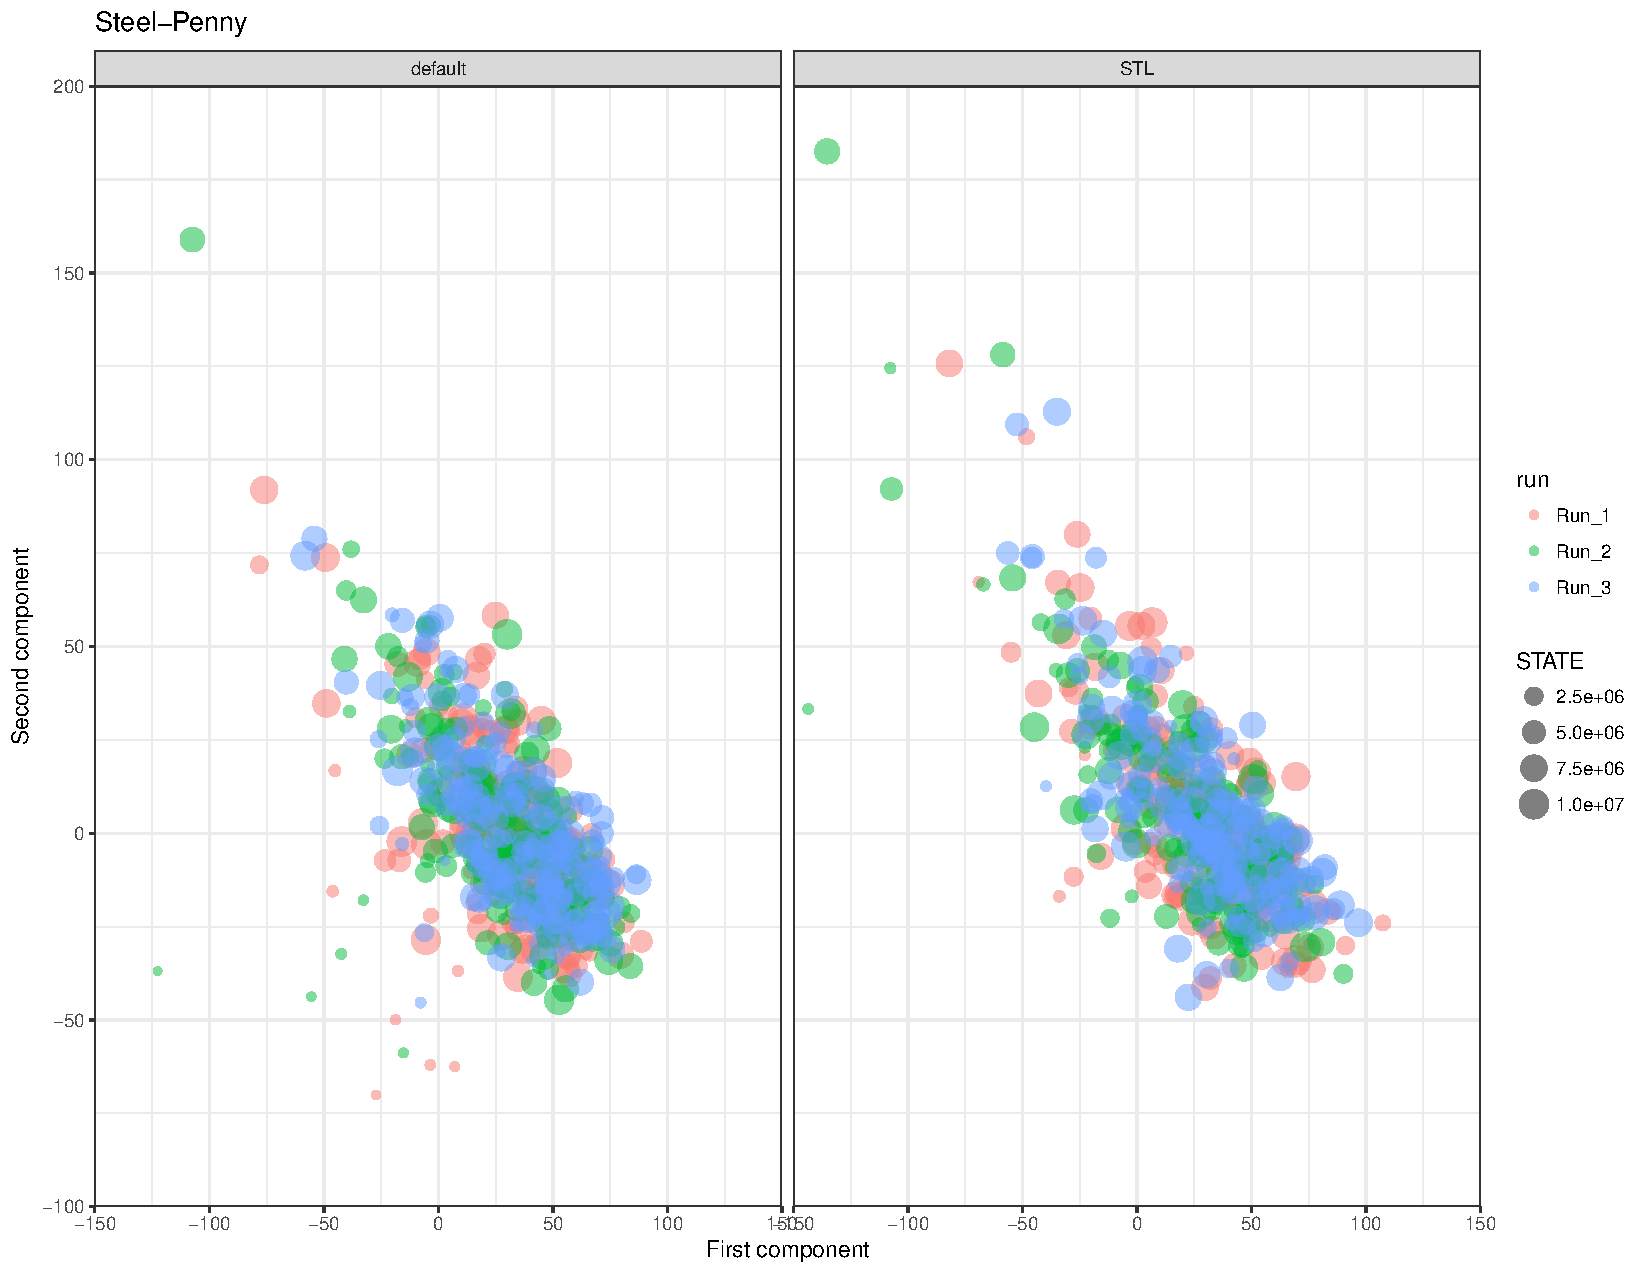
\includegraphics[scale=0.5]{\dir/figs/mds_ebov_SP.pdf} 
\end{center}
 \caption[MDS projections for the full EBOV 1610 taxa data set (Steel-Penny distances).]{\textbf{MDS projections for the full EBOV 1610 taxa data set (Steel-Penny distances).}
 I sampled 200  equally spaced trees from each chain (1200 trees in total) and computed the Steel-Penny distance~\citep{Steel1993} for every pair of trees.
 Colours relate to the seed used in the pseudo random number generator, ensuring each run starts from the same point. 
 See Figures~\ref{fig:mds_ebov_RF} and~\ref{fig:mds_ebov_KC} for projections of the same trees under different metrics.
 }
 \label{fig:mds_ebov_SP}
\end{figure}

One question seldom approached in the literature is the quality of MDS projections of phylogenetic space.
As mentioned above, it is standard practice to keep the first two components for plotting and analysis, but if this 2-d  projection is to be a faithful representation of the space of interest we need to ascertain that the first two components do indeed capture most of the variation.
A way of analysing the quality of the projections is to plot the scaled eigenvalues against the component number.
Ideally, the first few components capture most of the variation, resulting in an ``elbow-shaped'' plot.
In contrast, a flat plot suggests that variation is spread across many components and hence restricting attention to the first two can be misleading.
In Figure~\ref{fig:screeplots} I show these plots for a range of real-world data sets (see Table~\ref{tab:datasets} in Chapter 2).
A consistent result across data sets is the plot for the Robinson-Foulds (RF) distance, which is mostly flat and suggests that for this metric it is not sufficient to look at the first few components in order to get a good picture of the variation in the sample.

\begin{figure}[!ht]
\begin{center}
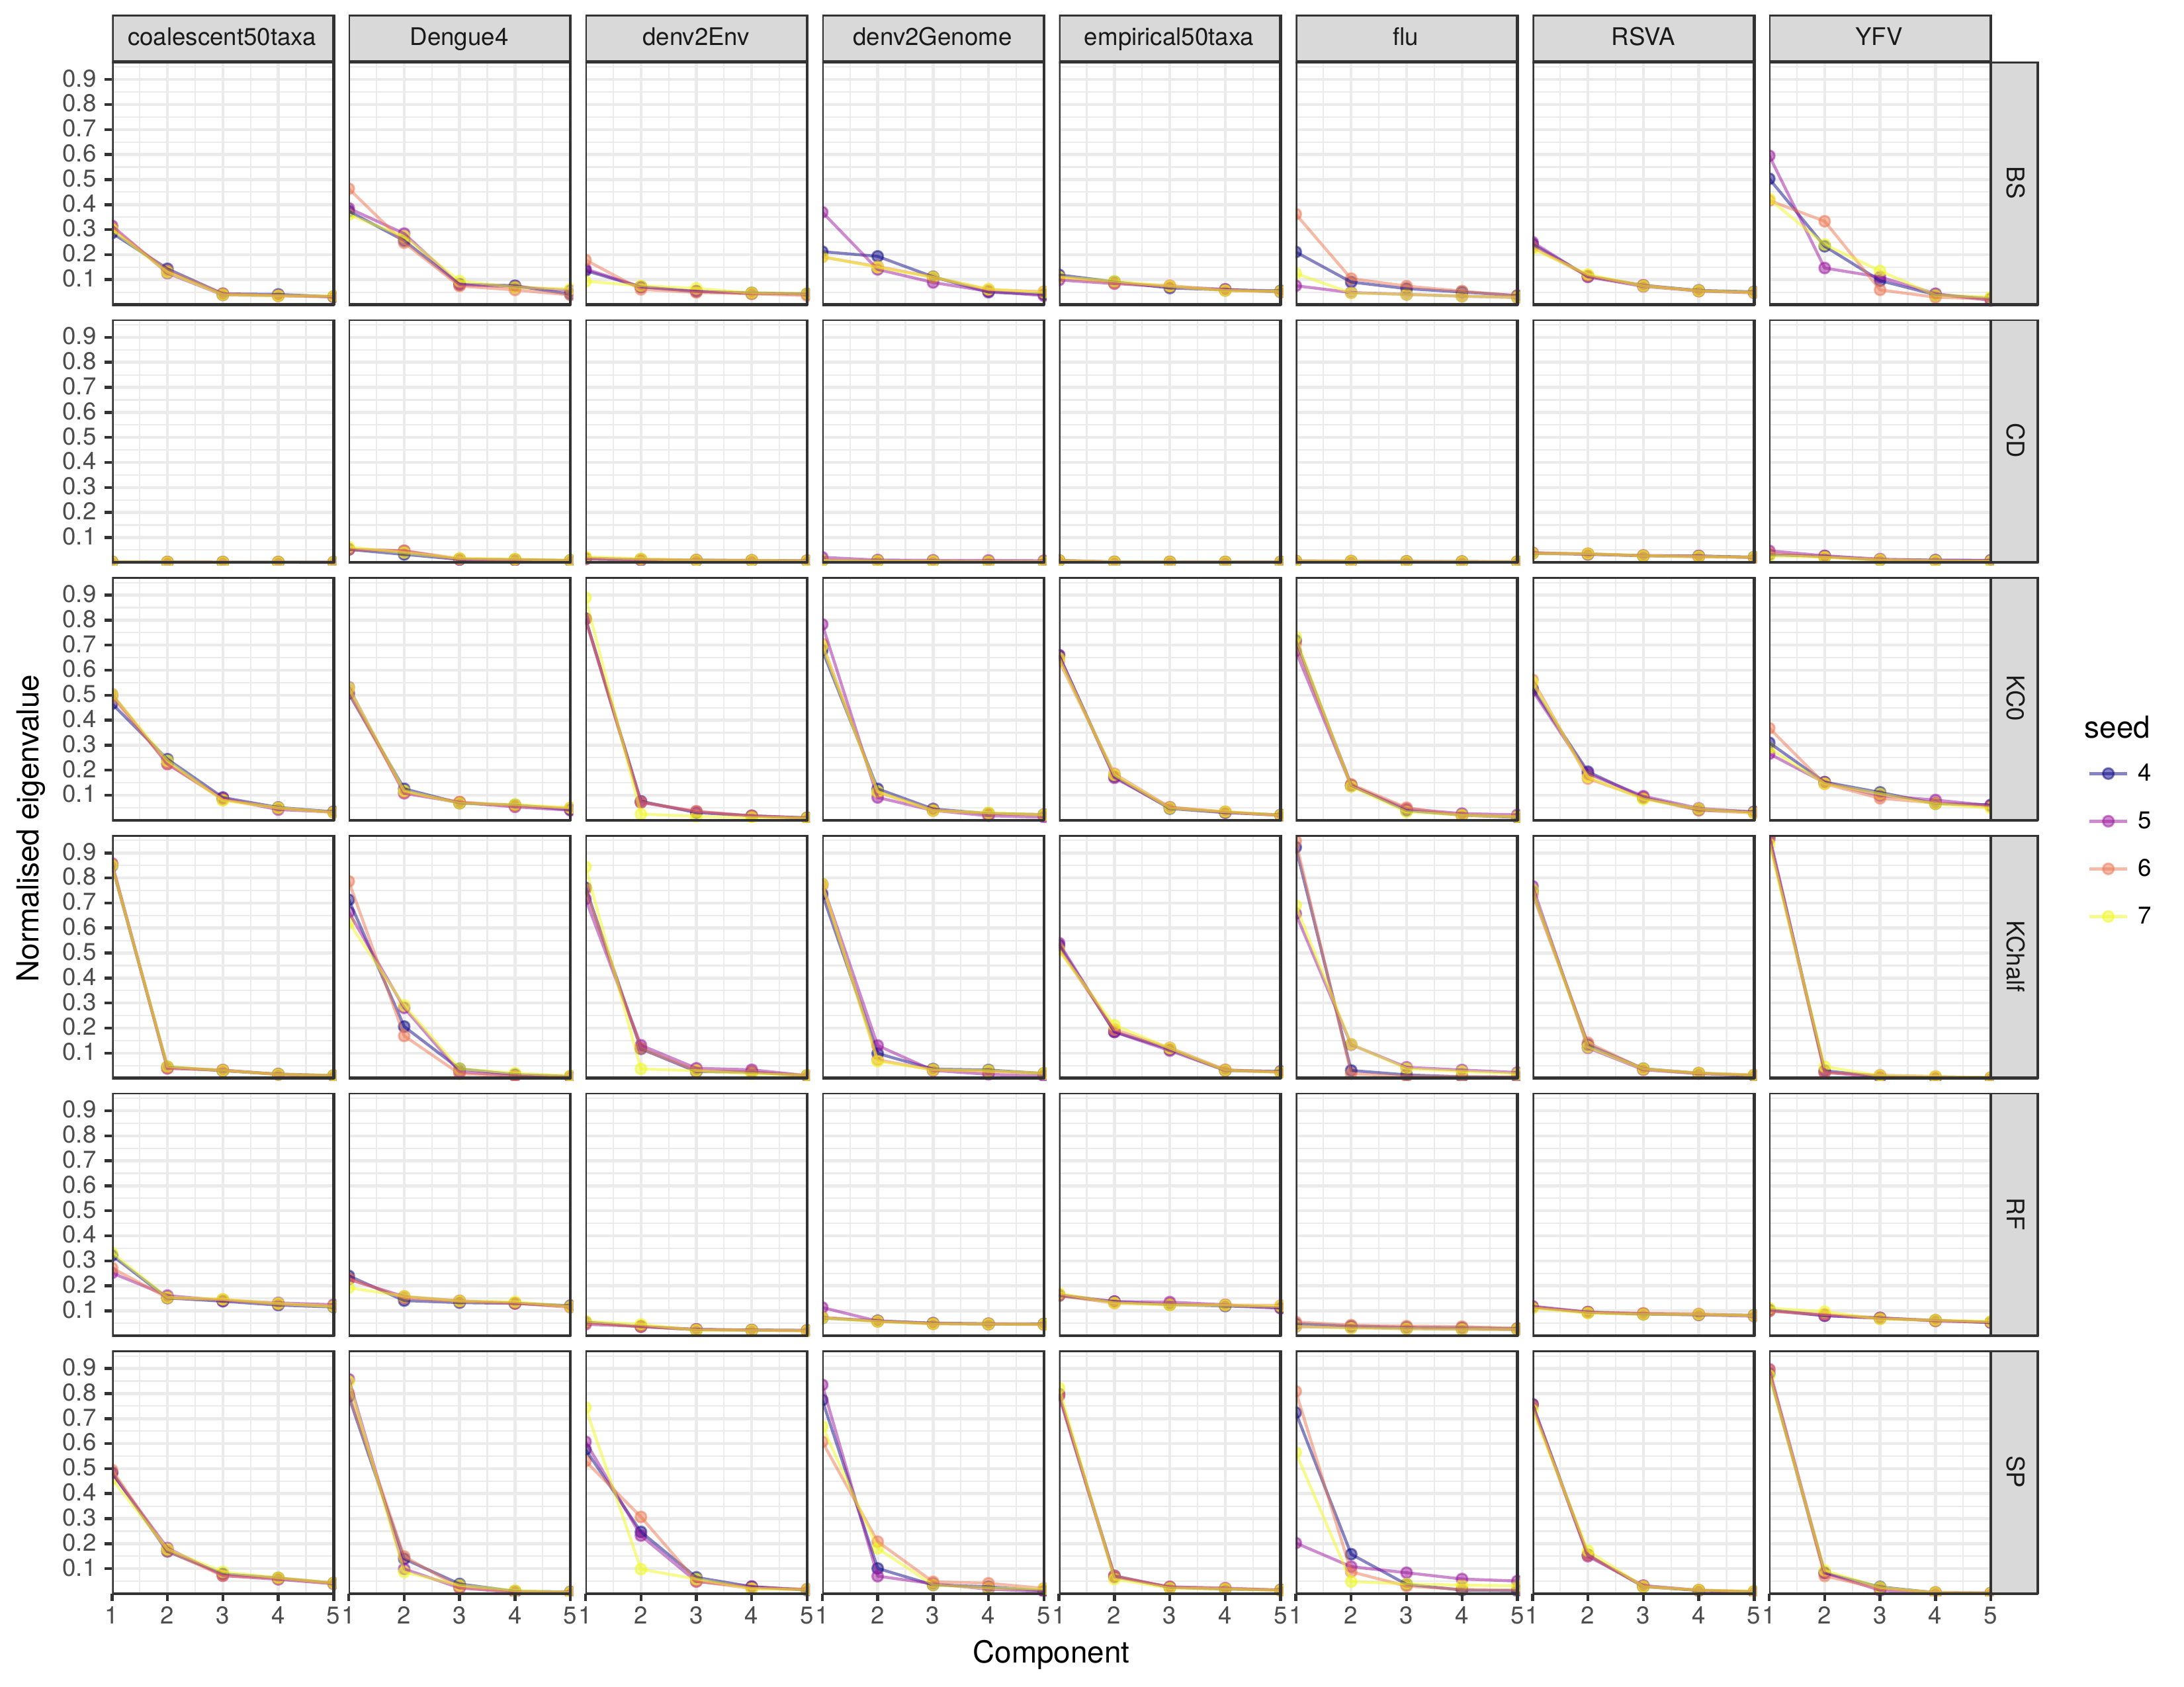
\includegraphics[scale=0.55]{\dir/figs/scree_plots_mds.png} 
\end{center}
 \caption[Scaled eigen values of phylogenetic space MDS.]{\textbf{Scaled eigen values of phylogenetic space MDS.}
 Vertical tiling shows the data set and horizontal ones show the phylogenetic metric used.
 Colours relate to the seed used in the pseudo random number generator, ensuring each run starts from the same point. 
 ``Elbow-shaped'' plots indicate fewer components are needed to capture the variation in the data.
 }
 \label{fig:screeplots}
\end{figure}

\subsection{Typical set for phylogenies}
\label{sec:typical}

One question one might ask is, what does phylogenetic space look like when we know the right answer?
In this section I offer a first stab at this question by analysing a simulated data example with $50$ taxa (Section~\ref{sec:simudata}).
I present trace plots of the distance to the true tree and MDS projections of the posterior distributions under various metrics, marking the maximum clade credibility (MCC) trees obtained from each run of each operator mix and the true tree used to generate the data.
In Figure~\ref{fig:mds_50taxa_RF}, I show the MDS projection of the RF distances between trees sampled using three MCMC schemes (``operator mixes'' or MCMC schemes, see Chapter 2), under two generating models: a tree drawn from the coalescent and an empirical tree extracted from a real-world data sets.
We can see that as the amount of data increases, the posteriors become more concentrated around the true value, as do the MCC trees, as expected.
While this behaviour is shared for both true trees (coalescent or empirical), the posteriors for the coalescent generating tree seem to be more variable.

\begin{figure}[!ht]
\begin{center}
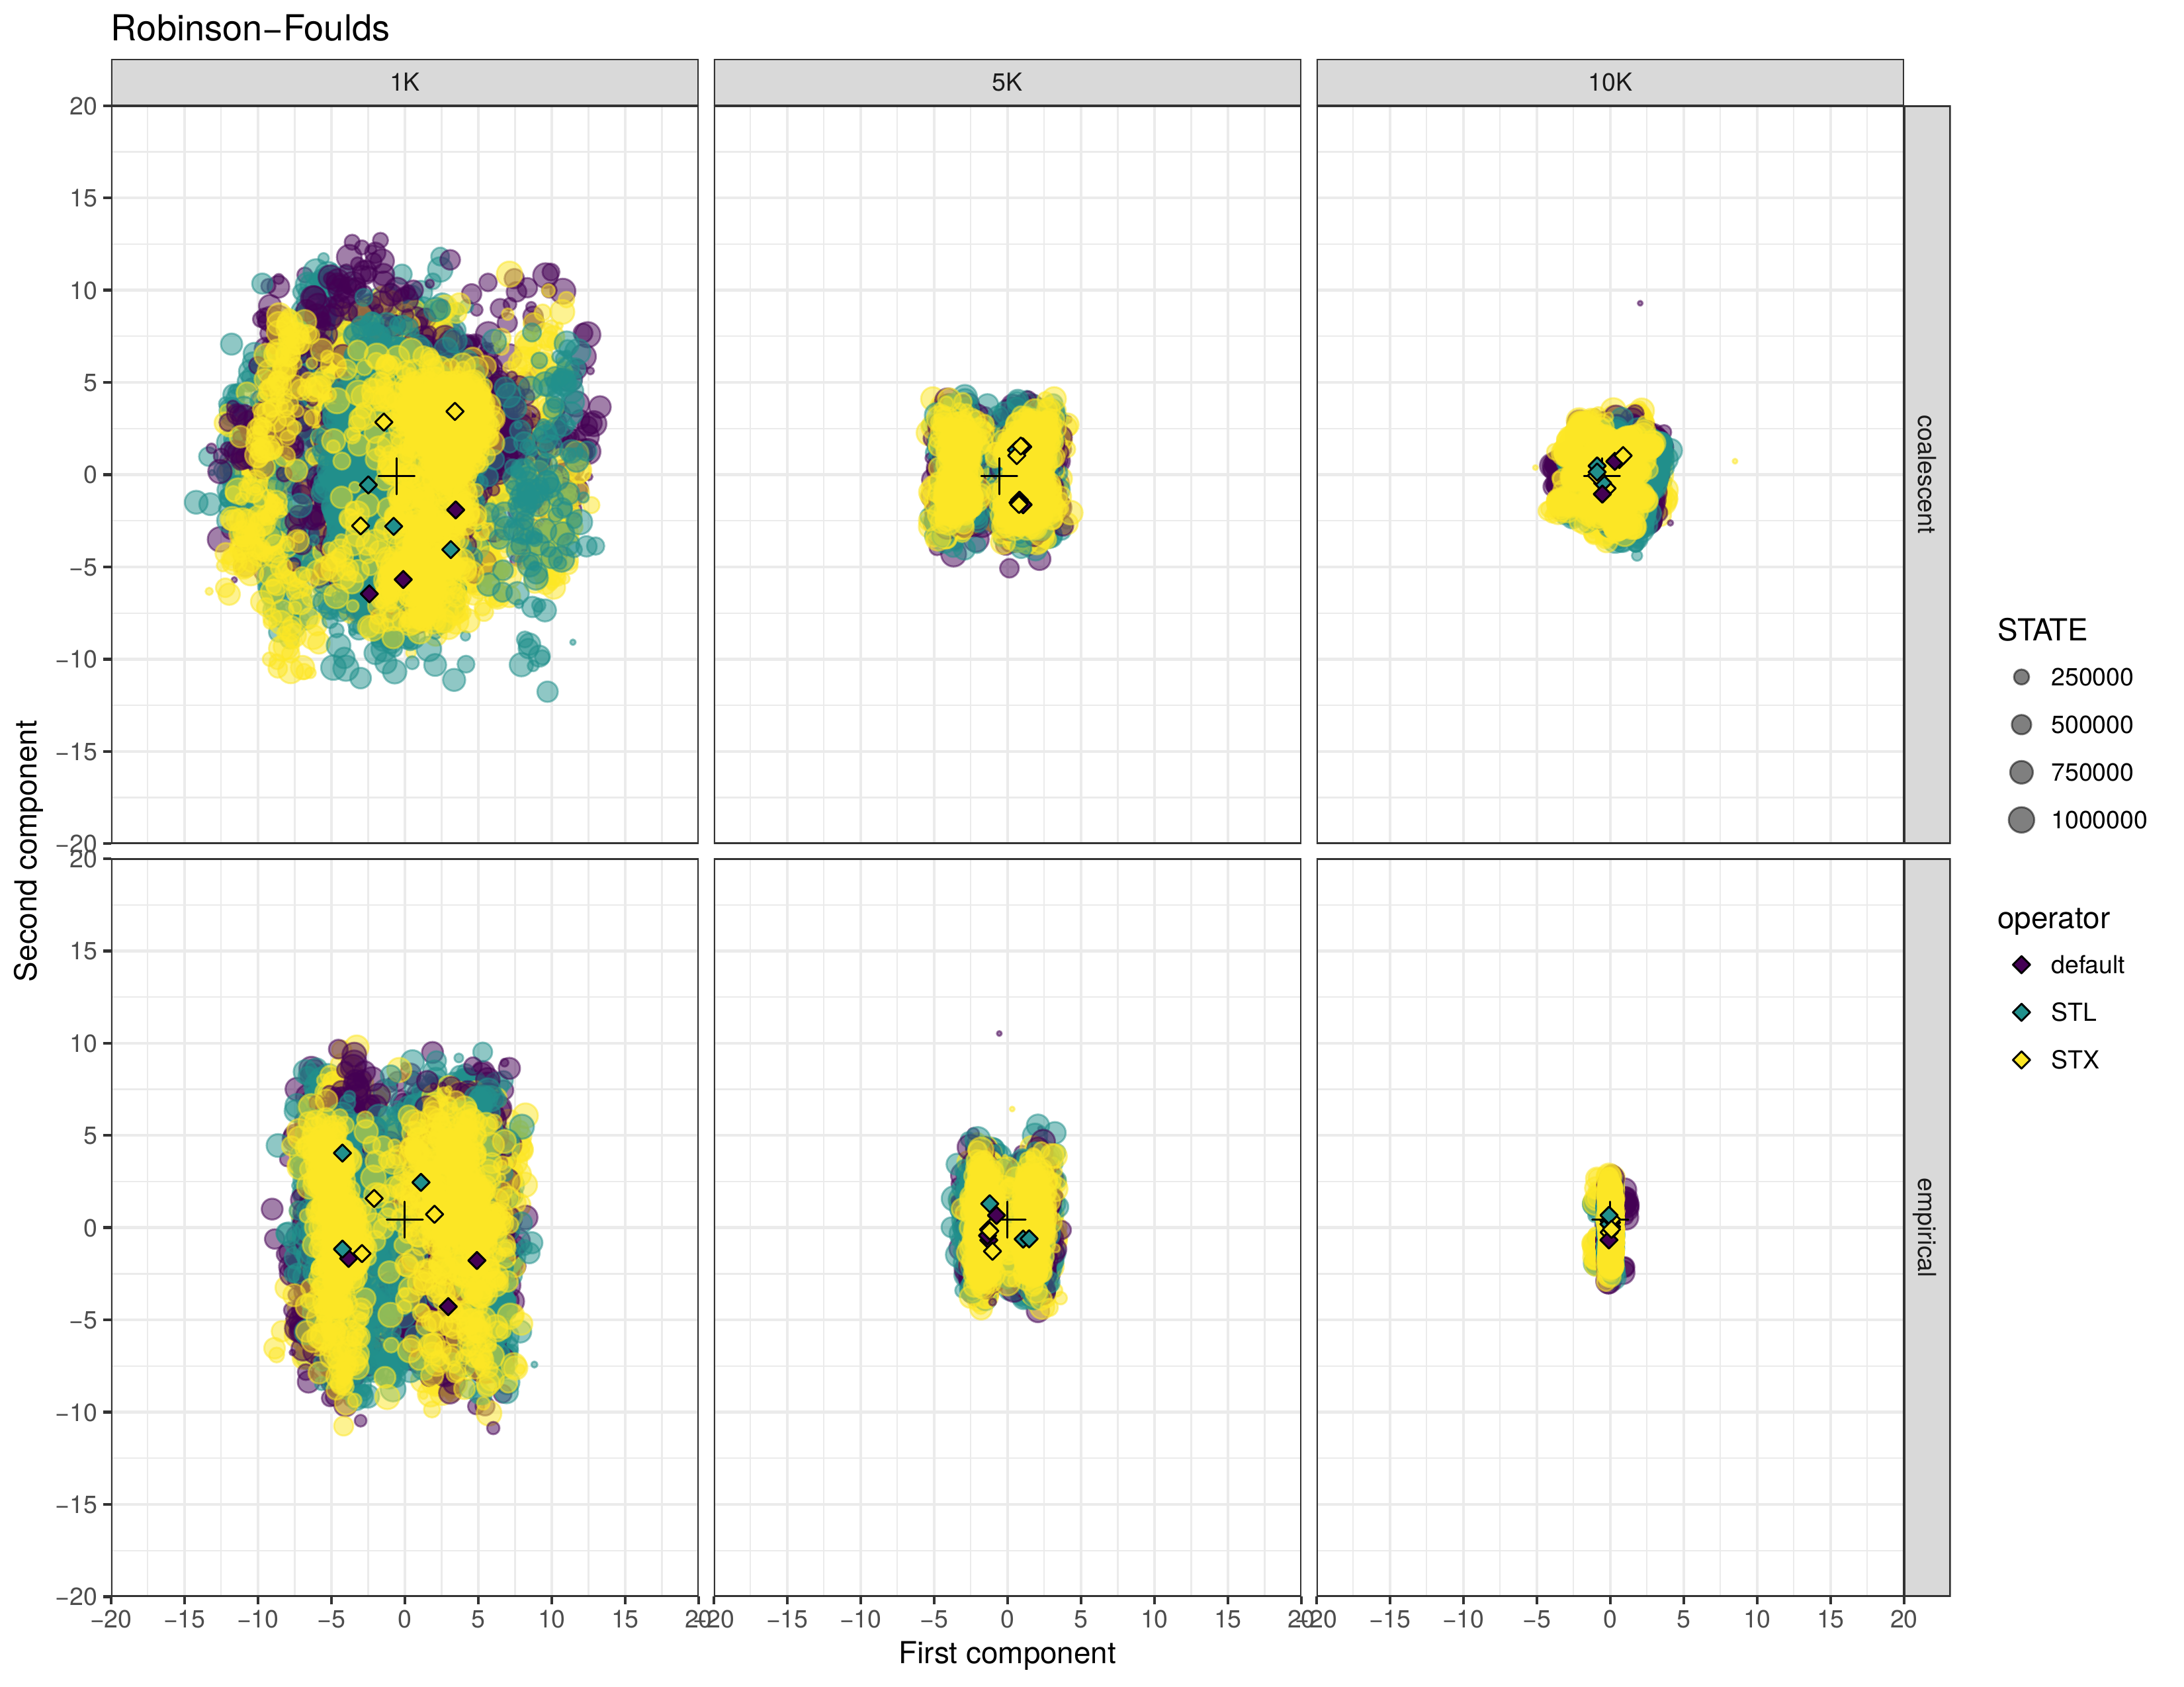
\includegraphics[scale=0.5]{\dir/figs/mds_50taxa_RF.png} 
\end{center}
 \caption[MDS projections for the simulated 50 taxa data set (Robinson-Foulds distances).]{\textbf{MDS projections for the simulated 50 taxa data set (Robinson-Foulds distances).}
  I show three replicates per operator, 1000 trees in each replicate, computing the RF distance between all pairs of trees.
 Colours pertain to the combination of MCMC transition kernels used and solid diamonds mark the maximum clade credibility (MCC) trees obtained from each run.
 Horizontal panels show the true tree: either drawn from the coalescent or extracted from a real world data set (``empirical'').
 Vertical panels show the number of sites in the simulated alignment (1000, 5000 or 10 000).
 Please see Section~\ref{sec:simudata} for more details.
 }
 \label{fig:mds_50taxa_RF}
\end{figure}

Under the KC metric with $\lambda = 0$ (Figure~\ref{fig:mds_50taxa_KC0}), we observe a very similar pattern, but for this data set this representation more clearly shows the topological modes and how the MCC trees approach the correct mode (that contains the true tree) as the amount of data grows (rightmost bottom panel) .
Also from this panel we see that the posterior for the empirical generating tree also show markedly separate modes when compared to coalescent generating tree.
Since this representation captures only topological features, I claim that the differences must be due to the implicit interaction between branch length distribution and topology. 
An interesting observation is that the default operators sometimes lead to samples outside the typical set even when the chain is supposed to have converged to the target (rightmost top panel).
\begin{figure}[!ht]
\begin{center}
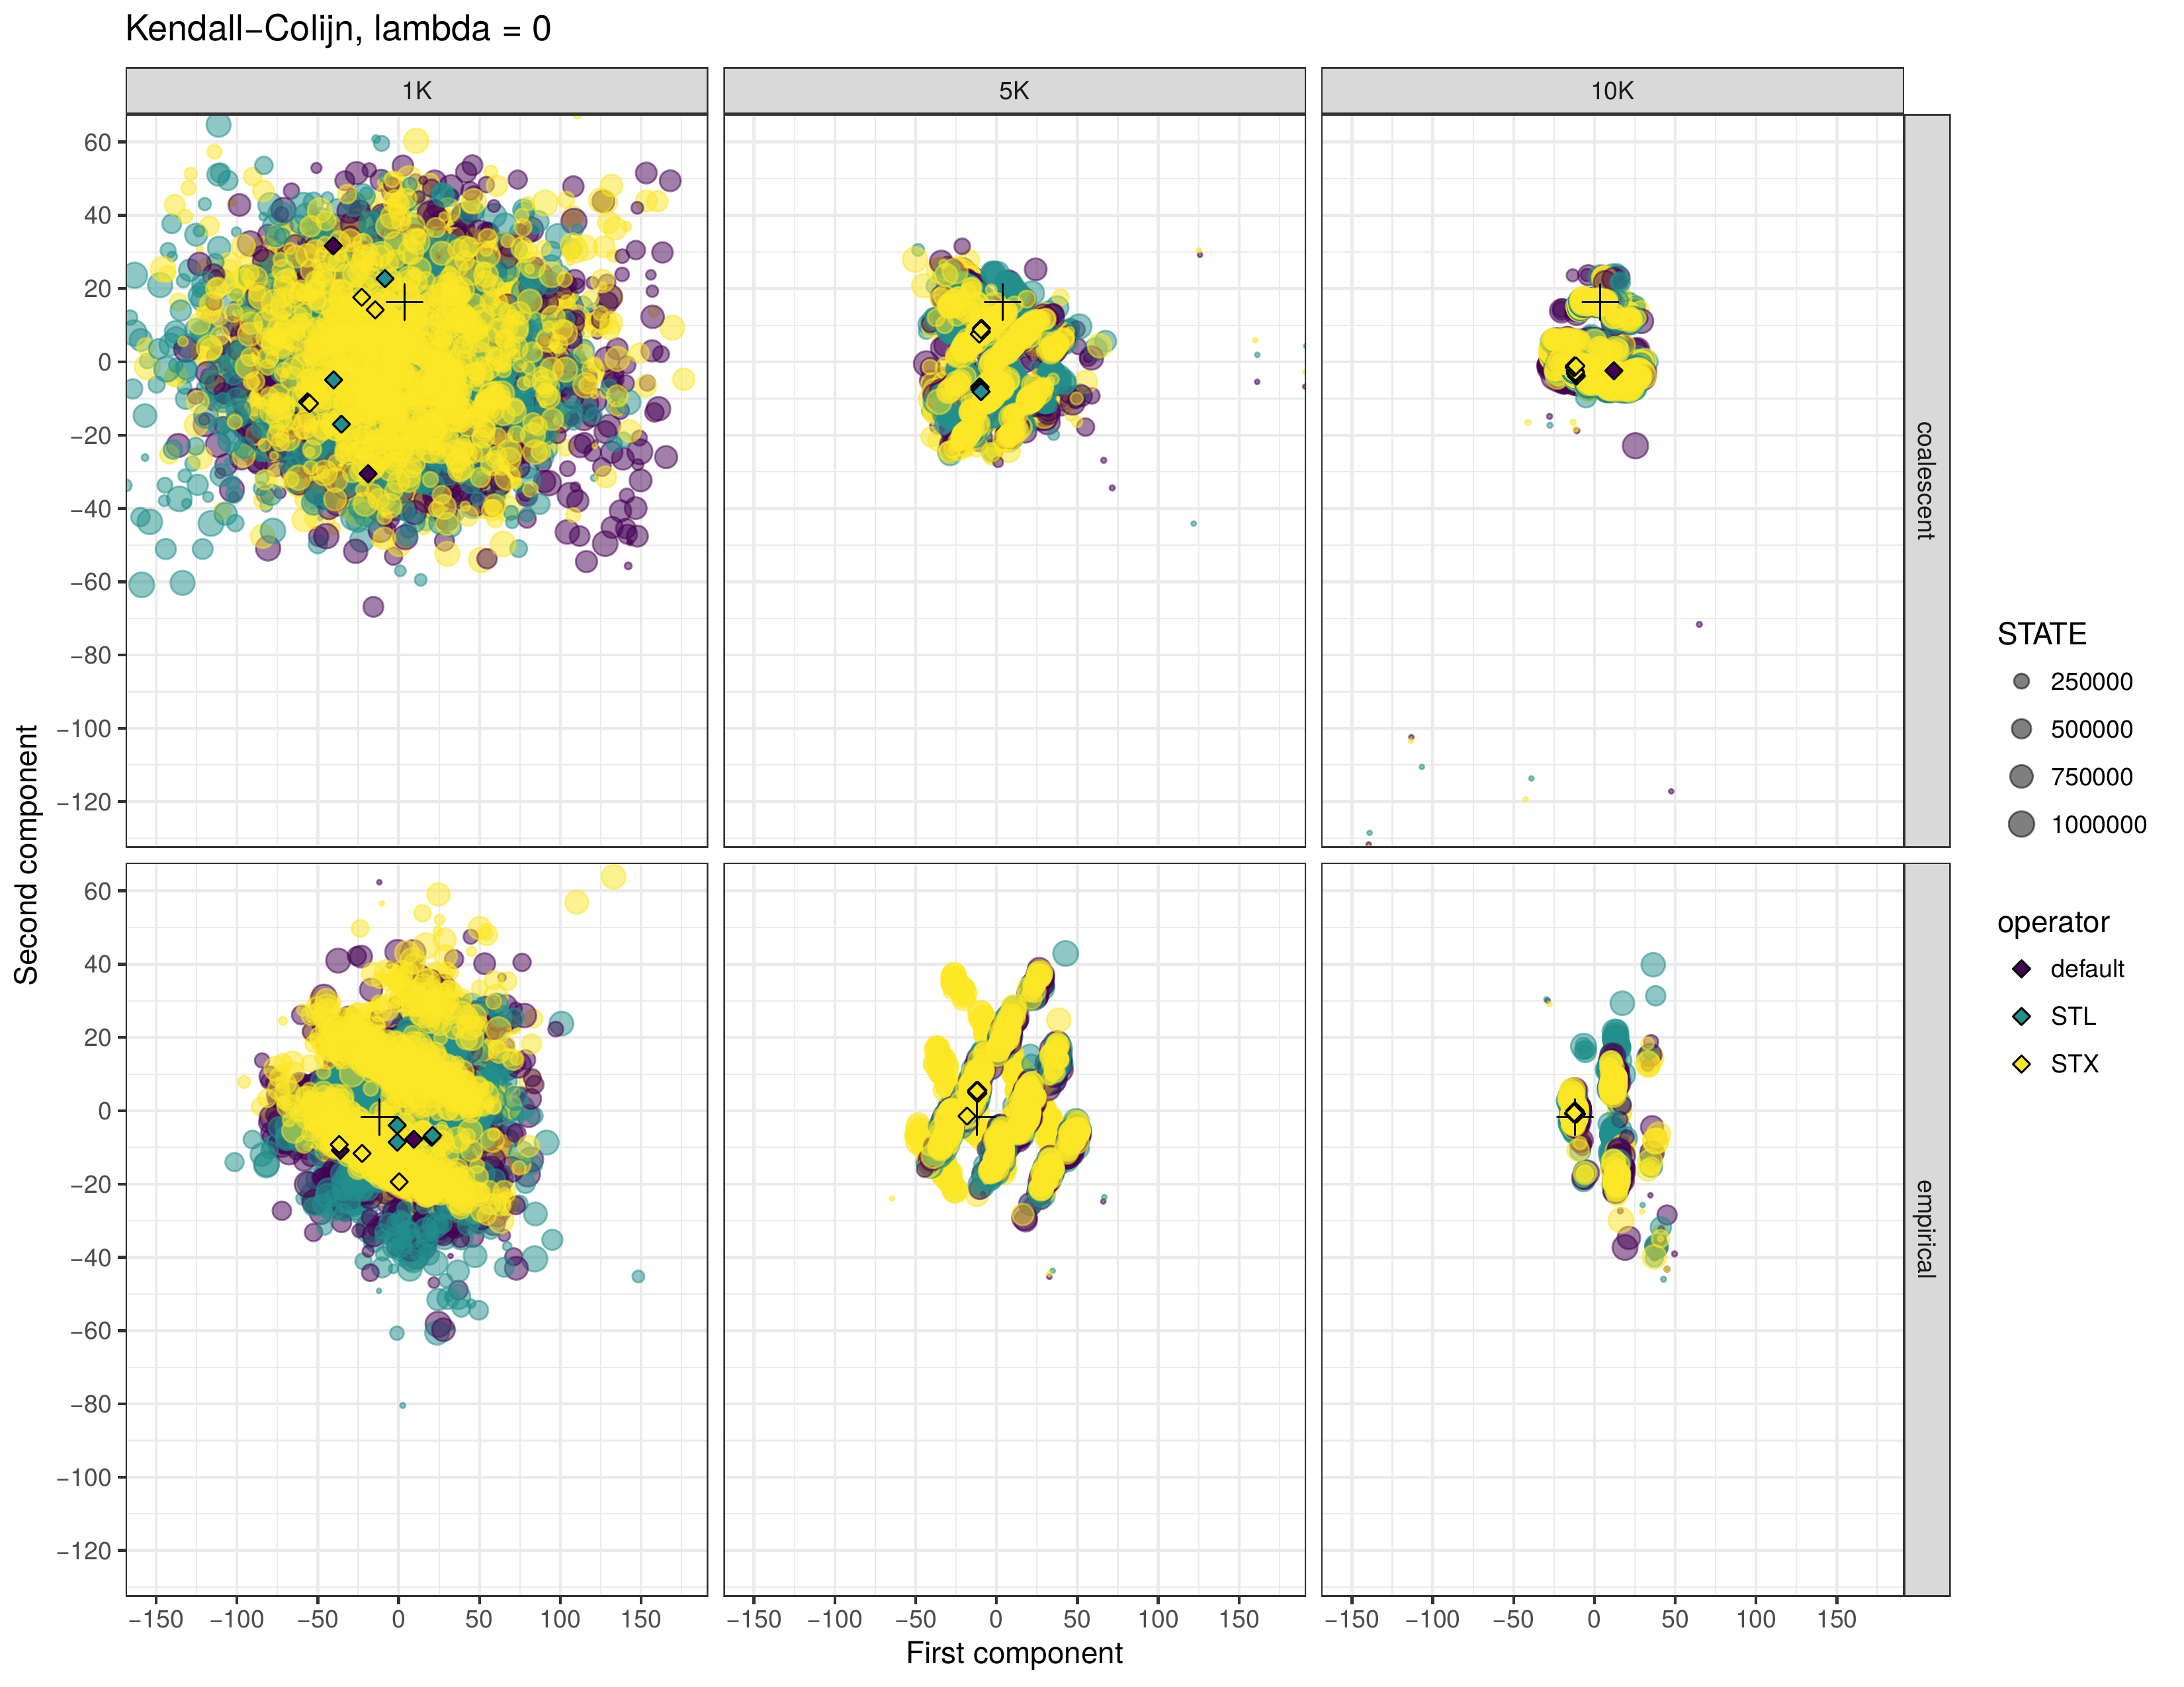
\includegraphics[scale=0.5]{\dir/figs/mds_50taxa_KC0.png} 
\end{center}
 \caption[MDS projections for the simulated 50 taxa data set (Kendall-Colijn distances).]{\textbf{MDS projections for the simulated 50 taxa data set (Kendall-Colijn distances).}
  I show three replicates per operator, 1000 trees in each replicate, computing the KC distance between all pairs of trees.
 Colours pertain to the combination of MCMC transition kernels used and solid diamonds mark the maximum clade credibility (MCC) trees obtained from each run.
 Horizontal panels show the true tree: either drawn from the coalescent or extracted from a real world data set (``empirical'').
 Vertical panels show the number of sites in the simulated alignment (1000, 5000 or 10 000).
 See Figure~\ref{fig:mds_50taxa_RF} for a projection of the same trees under the RF metric.
 }
\label{fig:mds_50taxa_KC0}
\end{figure}

In keeping with the results in Section~\ref{sec:representation}, the Steel-Penny metric leads to MDS projections that appear smoother (Figure~\ref{fig:mds_50taxa_SP}).
Also noteworthy is the amount of samples outside the typical set observed for the default kernels (small purple dots). 
Taken together with Figures~\ref{fig:mds_50taxa_RF} and~\ref{fig:mds_50taxa_KC0}, these results show progressive concentration of the posterior around the true value with alignment size (number of sites), even if posteriors for the empirical generating tree seem less smooth and harder to sample from.
\begin{figure}[!ht]
\begin{center}
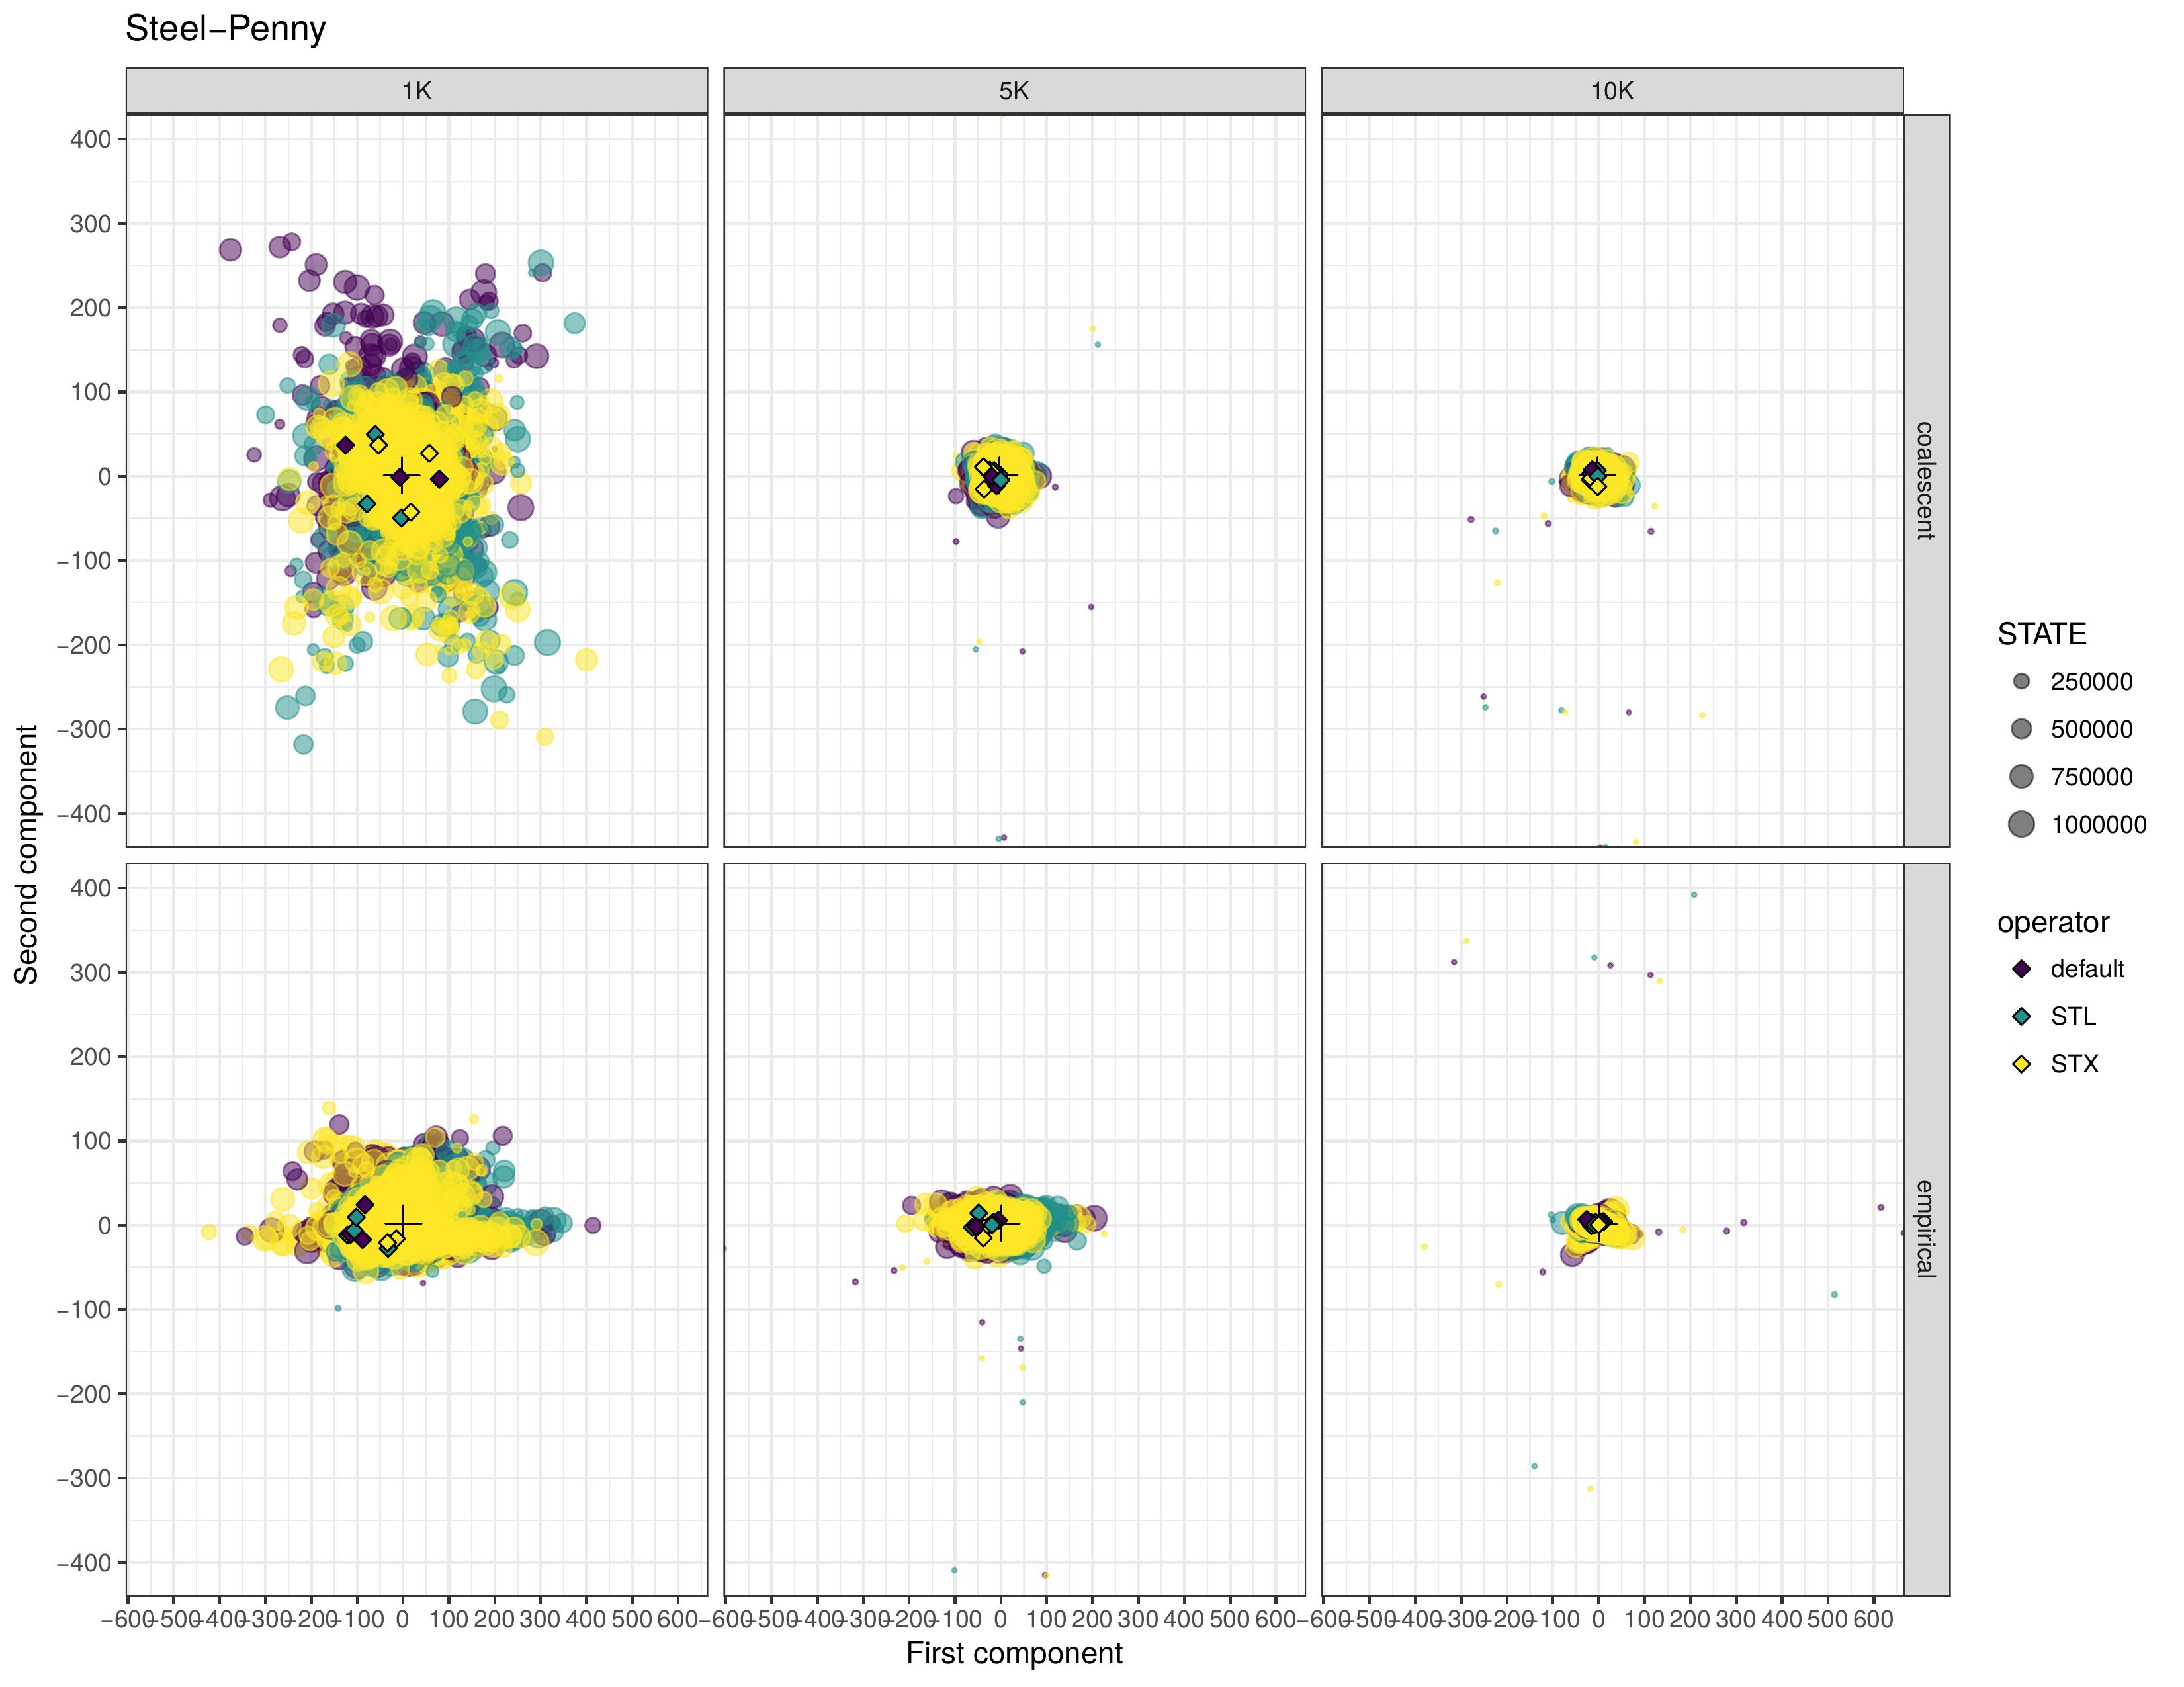
\includegraphics[scale=0.5]{\dir/figs/mds_50taxa_SP.png} 
\end{center}
 \caption[MDS projections for the simulated 50 taxa data set (Steel-Penny distances).]{\textbf{MDS projections for the simulated 50 taxa data set (Steel-Penny distances).}
 I show three replicates per operator, 1000 trees in each replicate, computing the SP distance between all pairs of trees.
 Colours pertain to the combination of MCMC transition kernels used and solid diamonds mark the maximum clade credibility (MCC) trees obtained from each run.
 Horizontal panels show the true tree: either drawn from the coalescent or extracted from a real world data set (``empirical'').
 Vertical panels show the number of sites in the simulated alignment (1000, 5000 or 10 000).
 See Figure~\ref{fig:mds_50taxa_RF} for a projection of the same trees under the RF metric.
 }
\label{fig:mds_50taxa_SP}
\end{figure}

When we know the true tree, we can also study phylogenetic space and its exploration by MCMC by computing the distance to the true tree and tracking how the distance changes through the chains as well as the resulting distributions.
In this simulated example we can exploit the fact that we know the true tree to the visualisation/analysis problem to essentially one dimension.
We can look at the resulting distributions as if they were univariate targets, which in turn facilitates visualisation and intuition-building, in addition to making it possible to apply a plethora of statistical methods developed for the analysis of univariate distributions.
While in practice we do not know the true tree, these simulations are useful for understanding the behaviour of transition kernels and MCMC in general. 

In Figure~\ref{fig:topo_distances_50taxa} I show the results of this analysis for the 50 taxa simulated example discussed above, for topological metrics (RF and KC)  in order to show the combinatorial (discrete) multimodality of phylogenetic space.
The first pattern to notice is that the number and location of peaks changes as the amount of information increases (colours).
Secondly, I highlight how running the chains for longer leads to better defined peaks, even though for this simple example\footnote{Recall that in this example the parameters are inferred under the generating model,\textit{i.e.} there is no model misspecification.} 10 million iterations seem to be adequate to find and explore all of the detected modes.
Also noticeable is how diffuse the target for the coalescent tree is for small alignment size (one thousand sites) under the KC metric (Figure~\ref{fig:topo_distances_50taxa}, panel D).
While the target intermediate alignment shows bimodality, the target for 10 thousand sites shows three modes, one much bigger than the other two.
Overall the empirical generating tree leads to more complex posteriors, specially for the intermediate alignment size (panel B, red curve).

\begin{figure}[!ht]
\begin{center}
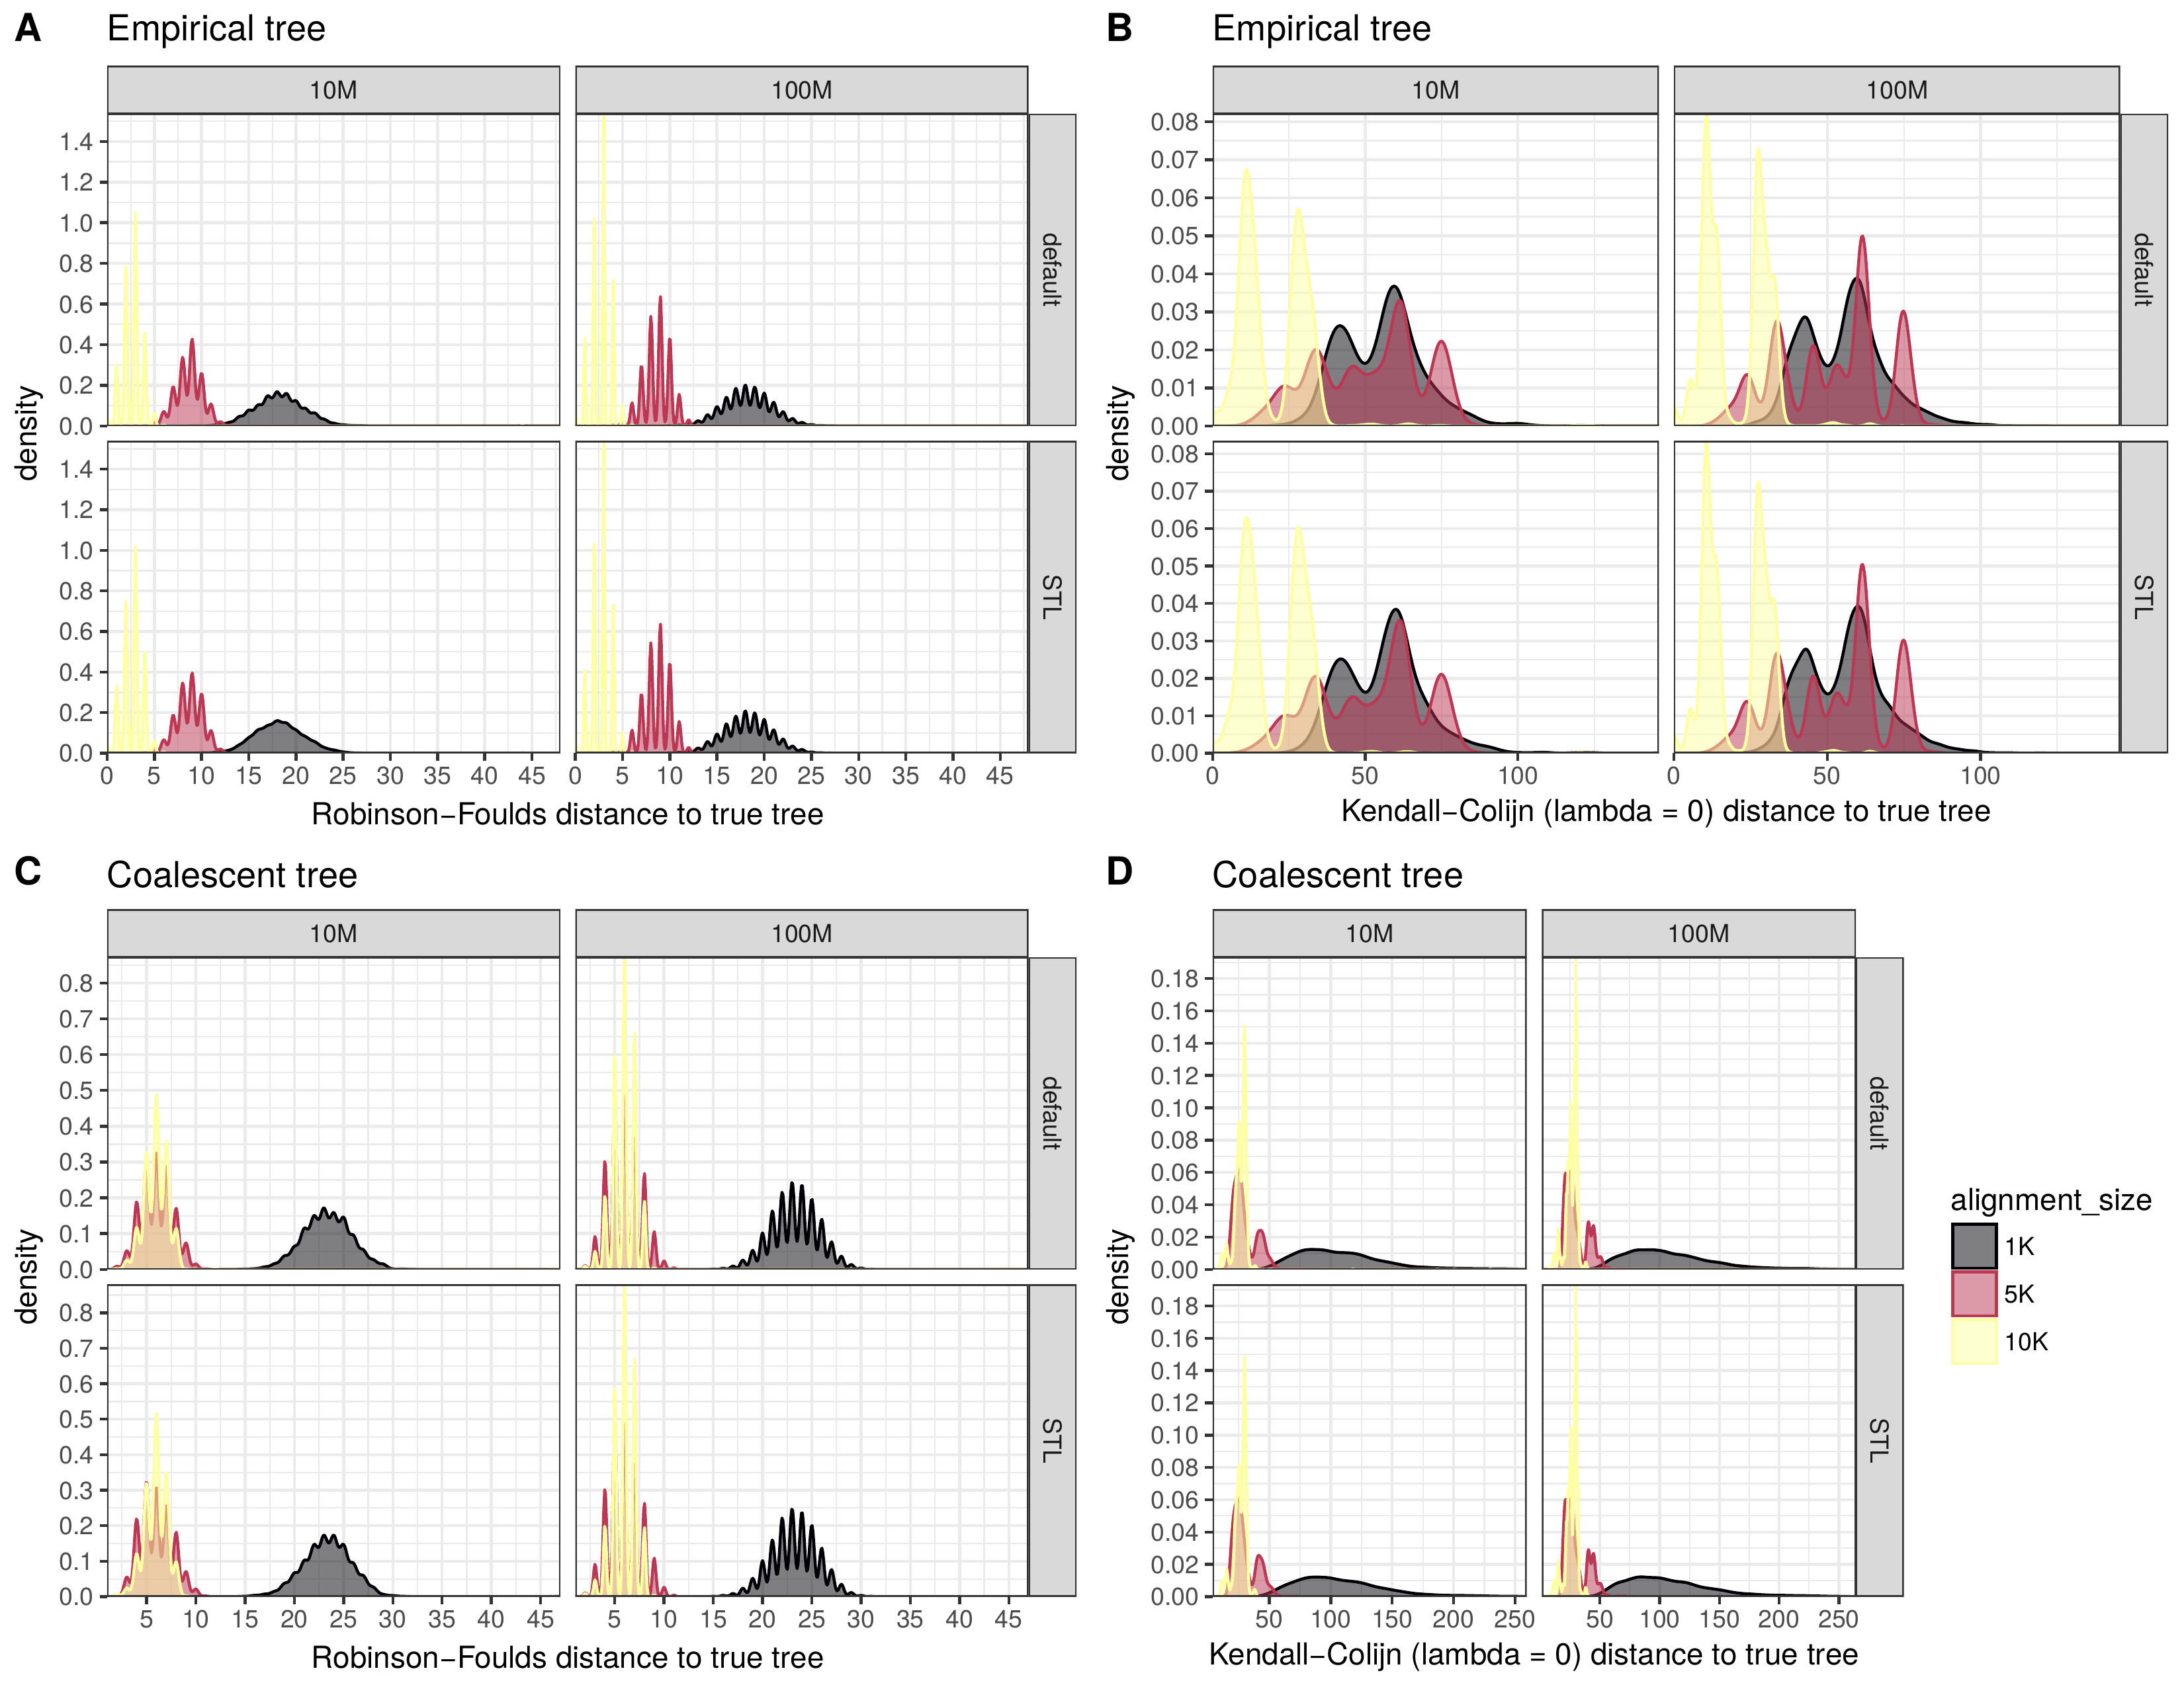
\includegraphics[scale=0.55]{\dir/figs/topo_distance_to_true_tree_50taxa.png} 
\end{center}
 \caption[Characterisation of topological modes for a simulated example (50 taxa).]{\textbf{Characterisation of topological modes for a simulated example (50 taxa).}
  I ran chains of 10 and 100 million iterations for three alignment sizes and two generating trees (see Chapter 2 for more details).
 Panels A and C show the Robinson-Foulds~\citep{Robinson1981} distance to the tree, while panels B and D show the Kendall-Colijn~\citep{Kendall2016} distance, with $\lambda =0$ (topology only). 
 Vertical panels show the chain length used, while horizontal panels display results obtained with different sets of transition kernels.
 }
 \label{fig:topo_distances_50taxa}
\end{figure}

When we turn attention to metrics that incorporate branch length information (Figure~\ref{fig:cont_distances_50taxa}), another interesting pattern emerges: while the SP metric leads to smooth targets, the KC metric shows distinct multimodality for the empirical generating tree.
It is difficult to say whether these observed differences are due to some underlying fundamental distinction or just an artefact specific to the two trees used -- there were not replicates at generating tree level of the experiment.
This result calls for further investigation into the inherent differences between empirical trees,~\textit{i.e.}, trees that are estimated from data encountered in practice, and their coalescent counterparts (see Section~\ref{sec:conclusion}).

\begin{figure}[!ht]
\begin{center}
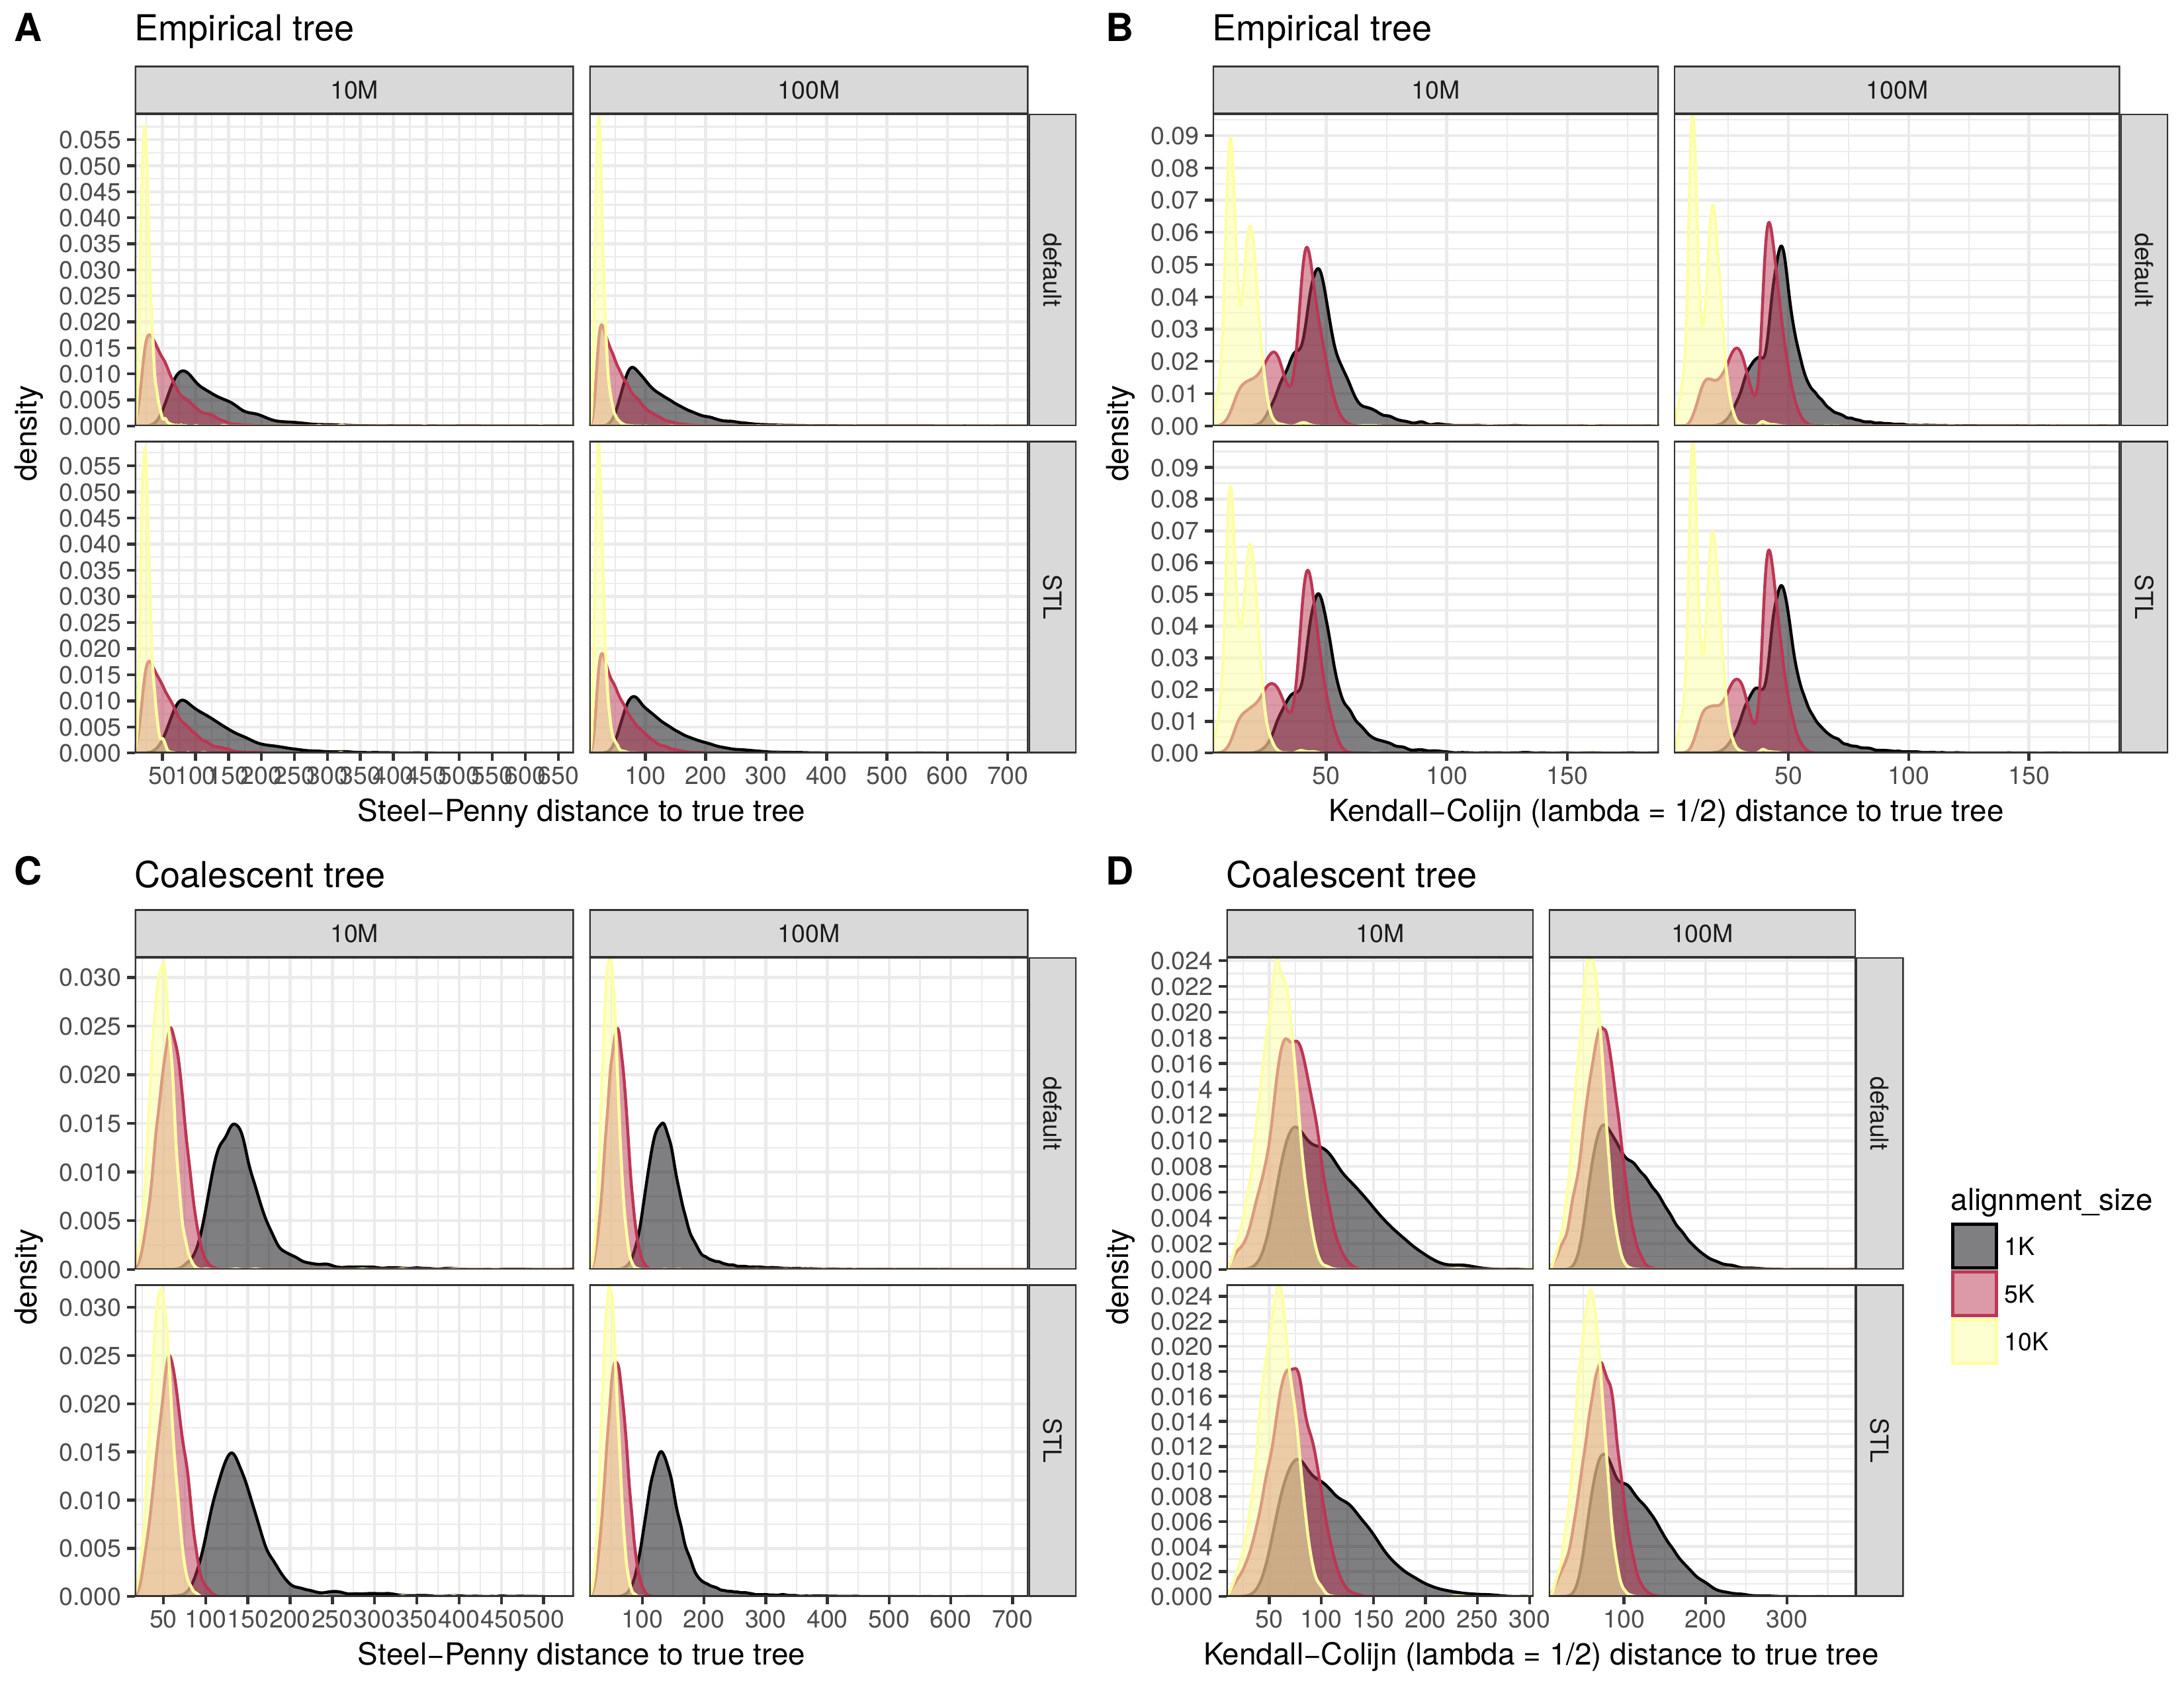
\includegraphics[scale=0.55]{\dir/figs/cont_distance_to_true_tree_50taxa.png} 
\end{center}
 \caption[Characterisation of continuous phylogenetic space for a simulated example (50 taxa).]{\textbf{Characterisation of continuous phylogenetic space for a simulated example (50 taxa).}
  I ran chains of 10 and 100 million iterations for three alignment sizes and two generating trees (see Chapter 2 for more details).
 Panels A and C show the Steel-Penny~\citep{Steel1993} distance to the tree, while panels B and D show the Kendall-Colijn~\citep{Kendall2016} distance with $\lambda = 1/2$,  which accounts for both topology and branch lengths. 
 Vertical panels show the chain length used, while horizontal panels display results obtained with different sets of transition kernels.
 }
 \label{fig:cont_distances_50taxa}
\end{figure}
Figures~\ref{fig:topo_distances_50taxa} and~\ref{fig:cont_distances_50taxa} also illustrate how casting the phylogeny sampling problem as a univariate sampling problem allows one to more clearly compare MCMC strategies.
Under both representations it is clear that \verb|SubTreeLeap| leads to virtually identical samples to those obtained with the default set of transition kernels, increasing confidence in the correctness of its implementation (see Chapter 2, Section~\ref{sec:correctness}). 
Moreover, it also seems to find and sample from all the detected modes, even for complex distributions such as those in panel B of Figure~\ref{fig:topo_distances_50taxa}.

While reducing the problem to a univariate quantity is an attractive idea (see, e.g. ``Method 1'' in ~\cite{Lanfear2016}), it is generally not possible in practice since we do not know the true tree and the choice of focal tree is arbitrary.
In the context of the development of phylogenetic transition kernels, however, I believe this method can be useful in constructing univariate representations of the target distribution, and thus allow us to leverage a vast body of theory available for assessing performance and correctness.
See Section~\ref{sec:mcmc_efficiency} in Chapter 2 for more details on how this  framework can be applied to evaluate MCMC mixing.

\section{Final remarks}
\label{sec:conclusion}

In this chapter I have sought to supplement the toolbox of diagnostic measures for MCMC in phylogenetic space with a few new tools and other tools seldom used in the field.
I by no means claim to have provided the first workflow of this kind, however.
Previous studies such as~\cite{Hillis2005},~\cite{Lakner2008},~\cite{Nylander2008} and~\cite{Warren2017} have touched on many of the aspects tackled here.
The research report here is an attempt at combining previous approaches with new metrics while overcoming some of the technical hurdles that large time-calibrated phylogenies impose.

The results for the ``poor'' runs (Table~\ref{tab:continuous_results}) are not surprising since the chain was deliberately designed to mix poorly in phylogenetic space.
A perhaps more subtle point to be made, however, is that since parameters vary regarding their inherent dependence on the phylogeny, computing global convergence metrics including all parameters might mask convergence problems.
This could be easily fixed by separating parameters into blocks when assessing convergence; more phylogeny-dependent parameters could be paid special attention.
Of course it is not always easy to know how dependent on the underlying phylogeny a parameter is; further research is needed in order to determine whether/how to do parameter blocking.
The multivariate ESS results show that when accounting for correlations between parameters none of the tested MCMC schemes achieves a sufficient number of samples.
This is intimately linked with the common recommendation of declaring a run acceptable if it achieves marginal univariate ESSs larger than $200$ for all parameters.
The practical relevance of this rule is yet another topic for future research.

Regarding diagnostics specifically designed for phylogenies, the results in Table~\ref{tab:tree_results} suggest a lack of agreement between approximate ESSs computed using different tree metrics.
For instance, for the poorly mixing runs some ESSs computed using the clade difference (CD) and branch score (BS) are estimated as 1001, the maximal value, suggesting these metrics might not be reliable for discriminating between poorly mixing runs and adequately mixing ones.
These results are in tune with those presented in Section~\ref{sec:representation}, which show that MDS projections under some metrics fail to highlight differences between runs and thus indicate severe convergence problems. 
In contrast, Figure~\ref{fig:ESS_distance_true} in Chapter 2 shows that pseudo-ESS seem consistent between metrics -- the ranking between MCMC schemes is largely consistent --, at least in a setting where the focal tree is a summary tree from the tail end of three independent (long) golden runs.
Clade-based metrics seem to provide more discriminating tools, albeit the experimental setup does not allow definitive claims to be made.
As discussed in Section~\ref{sec:cladeSwitch}, correlation structure between clades complicates diagnostics based on marginal quantities, what seems to be corroborated by the fact that for the poorly mixing runs the mean univariate ESS for clade indicators was around $800$, which could mislead researchers into inferring acceptable mixing.

These inconsistencies seem to stem from the non-standard nature of phylogenetic space, which admits many representations without any one way of depicting the space being canonical.
The Billera-Holmes-Vogtman (BHV,~\cite{Billera2001}) cubical complex representation is a good candidate with good statistical properties, but distances are hard to compute, while others such as Kendall-Colijn metric are easier to compute but suffer from poor statistical and/or theoretical properties.
The KC metric for example suffers from an inherent scaling problem: when branch lengths and node indices are not commensurate, it is hard to calibrate $\lambda$ in order to obtain interpretable results.
A study in the same vein as~\citep{Kuhner2014} to compare the relative efficiency of tree metrics specifically for time-calibrated phylogenies is sorely needed.

The attentive reader will have noticed that while I mention and describe the BHV (geodesic) metric and associated space, none of my results include this metric.
This deserves explanation.
While conceptually I believe the BHV representation of phylogenetic space to be the most complete, enjoying many desirable properties (see~\cite{Billera2001},~\cite{StJohn2017} and~\cite{Dinh2016}), despite recent advances in the computation of the BHV metric~\citep{Owen2011} it still remains quite hard to apply to large time-trees.
Further programming work is needed to integrate the libraries provided by~\citep{Owen2011} into the framework described in this chapter.
In addition, if we are to approach phylogenetic inference as a statistical problem~\citep{Holland2013}, we need a representation that is statistically motivated so that results such as central limit theorems can be established.
Under such a representation, concepts such as effective sample sizes and typical sets are easier to interpret and analyse.
See Chapter 6 for a discussion of how BHV-based representations can be extended in that direction.

In summary, this chapter provides the following contributions/findings:
\begin{itemize}
 \item New analytical tools for a robust Bayesian phylogenetic analysis pipeline;
 \item For a given data set, some metrics can completely fail to indicate important differences between runs (compare Figures~\ref{fig:mds_ebov_RF},~\ref{fig:mds_ebov_KC} and~\ref{fig:mds_ebov_SP});
 \item Depending on the data set and metric, using just the first two components can be misleading (Figure~\ref{fig:screeplots});
 \item Approximate tree ESSs based on different metrics (distances) gave inconsistent results;
\end{itemize}

Several questions remain open however, which I intend to tackle in future research:

\begin{itemize}
 \item How exactly does sampling affect (the exploration of) phylogenetic space?
 The results in Section~\ref{sec:typical} suggest that, for a highly idealised situation (relatively few taxa, no model misspecification) the typical set of topologies under most metrics is smooth and well-behaved, with posterior concentration around the true tree as alignment size increases and the MCC tree closer to the true data generating tree.
 It remains to be seen how model misspecification, for instance, changes these findings.
 \item Are there good universal  -- data set independent -- cut-offs for ASDSF? What about the clade switching score?
 Tracking clades can be an efficient way of counteracting the superexponential growth in the dimensionality of the parameter space, since the space of clades grows much slower.
 However, non-trivial correlations between clades mean that naive metrics that do not take this correlation into account will fail to spot nonconvergence.
 The ``holy grail'' of  MCMC for phylogenies convergence assessment is to find a cheap, preferably univariate measure that captures convergence with high sensitivity.
 \item Is it possible to elect one particular metric as more appropriate for the analysis of time-calibrated phylogenies?
 As mentioned above, a study extending the results of~\citep{Kuhner2014} to time-calibrated phylogenies would be a good contribution.
 Such a study would have to consider how to incorporate the serially sampling structure of tips into the experimental design, seeing as the sampling dates of the tips impose constraints not only on topology but also on branch lengths~\citep{Moller2018}.
\end{itemize}

% \bibliography{/home/max/Dropbox/PHD/THESIS/bibliography/lmcarvalho_PhD_Thesis}

%========================= Appendix ========================= 
\renewcommand{\chaptermark}[1]{%
 \markboth{\MakeUppercase{%
 \appendixname} \ \thechapter.%
 \ #1}{}}
%\renewcommand{\dir}{../appendix/appendix}
%\input{\dir/appendix.tex}

%========================= BIBLIOGRAPHY ========================= 
\ifthenelse{\boolean{edthesis}}
 {
 \begin{singlespace}
}
{
  \backmatter
}
\def\bibname{References}
% \tocotherhead{References}
% \addcontentsline{toc}{chapter}{References}
\bibliography{../bibliography/lmcarvalho_PhD_Thesis}
\ifthenelse{\boolean{edthesis}}
 {
  \end{singlespace}
 }{}


\end{document}
